\documentclass[11pt,oneside]{book} % Standard book format with 10pt font


% =============================================
%  Encoding and Fonts
% =============================================
\usepackage[utf8]{inputenc} % UTF-8 encoding for compatibility
\usepackage{lmodern}        % Latin Modern for improved scaling and clarity
\usepackage{microtype}      % Enhances spacing and readability
\usepackage{amsmath, amssymb}

% ---- Sans-Serif Font (Helvetica) ----
\usepackage{helvet}              % Use Helvetica for a modern sans-serif look
\renewcommand{\familydefault}{\sfdefault}  % Set sans-serif as the default font

% ---- Monospace Font (Fira Code) ----
\usepackage[T1]{fontenc}  % Ensure proper font encoding
\usepackage{FiraMono}      % Use Fira Mono for monospaced text
%\renewcommand{\ttdefault}{firamono} % Apply Fira Code globally to monospace
\renewcommand{\ttdefault}{zi4} % Apply Fira Code globally to monospace

% =============================================
%  Graphics and Colors
% =============================================
\usepackage{graphicx} % Enables image handling
\usepackage[table]{xcolor}
\usepackage{colortbl}        % explicitly load colortbl for table colors
\usepackage{longtable}

% fixing latex3 bug: 
%\makeatletter
%\providecommand{\g__tbl_row_int}{0}
%\makeatother

% ---- Define DWD-Inspired Colors ----
\definecolor{DWDblue}{RGB}{0,68,136}     % Primary DWD blue
\definecolor{dwdspecial}{RGB}{50,30,80}  % Slightly lighter blue for contrast
\definecolor{dwdblue}{RGB}{0,68,136}     % Alternative DWD blue (identical to primary)
% Define Colors
\definecolor{codegreen}{rgb}{0.0, 0.5, 0.0} % Dark green for comments
\definecolor{codeblue}{rgb}{0.0, 0.2, 0.6} % Muted dark blue for keywords
\definecolor{codered}{rgb}{0.6, 0.1, 0.1}  % Muted red for strings
\definecolor{codegray}{rgb}{0.4, 0.4, 0.4} % Gray for numbers and operators
\definecolor{backcolor}{rgb}{0.97, 0.97, 0.97} % Very light gray background
%\definecolor{DWDblue}{rgb}{0, 0.35, 0.7} % Define DWDblue
% Define a light blue color
\definecolor{lightblue}{RGB}{220, 230, 241} % Light blue for alternating rows
\definecolor{headerblue}{RGB}{180, 200, 230} % Slightly darker blue for headers
\definecolor{appendixblue}{RGB}{200, 220, 240} % Blue for appendix header


% --- Page Geometry ---
\usepackage[margin=1in]{geometry}

% --- Fancy Headers ---
\usepackage{fancyhdr}
\pagestyle{fancy}
\fancyhf{}
\fancyhead[L]{\nouppercase{\leftmark}}
\fancyhead[R]{\nouppercase{\rightmark}}
\fancyfoot[C]{\thepage}
% Update chapter and section marks for header display
\renewcommand{\chaptermark}[1]{\markboth{Chapter \thechapter: #1}{}}
\renewcommand{\sectionmark}[1]{\markright{Section \thesection: #1}}

% --- Section and Chapter Title Formatting ---
\usepackage{titlesec}
\titleformat{\chapter}[display]
  {\normalfont\Huge\bfseries\color{DWDblue}}
  {\chaptertitlename\ \thechapter}{20pt}{\Huge}
  
\titleformat{\section}
  {\normalfont\Large\bfseries\color{DWDblue}}
  {\thesection}{1em}{}

%\usepackage[utf8]{inputenc}

% --- For Dummy Text ---
\usepackage{lipsum}

\fancyhead[R]{
\includegraphics[width=0.2\textwidth]{images/DWD-Logo_2013.svg.png}}
\setlength{\headsep}{40pt}  % Adjust the value as needed

\usepackage{listings}
\usepackage[listings, breakable]{tcolorbox} % Enable listings inside tcolorbox
%\usepackage{xcolor}
\usepackage{accsupp}

\lstdefinelanguage{Markdown}{
  morekeywords={[1]\#,\#\#,\#\#\#,\#\#\#\#},
  morekeywords={[2]*,**,---,-},
  sensitive=false,
  morecomment=[l][\color{gray}]{<!--},
  morestring=[b]",
}

\lstdefinestyle{mdstyle}{
  language=Markdown,
  basicstyle=\ttfamily\small,
  breaklines=true,
  keywordstyle={[1]\color{blue}\bfseries},
  keywordstyle={[2]\color{purple}},
  commentstyle=\color{gray},
  stringstyle=\color{orange},
}

% Define the Python syntax highlighting style
\lstdefinestyle{pythonstyle}{
    language=Python,
    basicstyle=\ttfamily\small,    % Monospace font
    keywordstyle=\color{codeblue}\bfseries, % Keywords in blue
    stringstyle=\color{codered},  % Strings in red
    commentstyle=\color{codegreen}\itshape, % Comments in green italics
    numberstyle=\tiny\color{codegray}, % Line numbers in gray
    backgroundcolor=\color{gray!5}, % Light gray background
    breaklines=true,
    columns=fixed,
    showspaces=false,
    showstringspaces=false,
    keepspaces=true,
    numbers=left, % Show line numbers
    numbersep=5pt, % Adjust separation between numbers and text
    xleftmargin=7pt, % **Fix: Keeps numbers inside the box**
    framexleftmargin=15pt, % **Fix: Adds padding inside the box for numbers**
}

\lstdefinestyle{outputstyle}{
    language=Python,
    basicstyle=\ttfamily\small,    % Monospace font
    keywordstyle=\color{codeblue}, % Dark blue for keywords
    stringstyle=\color{codered},   % Muted red for strings
    commentstyle=\color{codegreen}\itshape, % Dark green italic for comments
    numberstyle=\color{codegray},  % Gray for numbers
    backgroundcolor=\color{backcolor}, % Light gray background
    breaklines=true,
    columns=fullflexible,
    showspaces=false,
    showstringspaces=false,
    keepspaces=true,
    xleftmargin=5pt, % Moves the entire box to the right
    framexleftmargin=5pt, % Keeps the frame aligned inside the box
}

% Define the Python syntax highlighting style
\lstdefinestyle{pythonstyle2}{
    language=Python,
    basicstyle=\ttfamily\small,    % Monospace font
    keywordstyle=\color{codeblue}\bfseries, % Keywords in blue
    stringstyle=\color{codered},  % Strings in red
    commentstyle=\color{codegreen}\itshape, % Comments in green italics
    numberstyle=\tiny\color{codegray}, % Line numbers in gray
    backgroundcolor=\color{gray!5}, % Light gray background
    breaklines=true,
    columns=fixed,
    showspaces=false,
    showstringspaces=false,
    keepspaces=true,
    numbers=none, % Show line numbers
    numbersep=5pt, % Adjust separation between numbers and text
    xleftmargin=7pt, % **Fix: Keeps numbers inside the box**
    framexleftmargin=15pt, % **Fix: Adds padding inside the box for numbers**
}


\newcommand{\includeexternalcode}[2]{%
  \begin{tcolorbox}[breakable,
    colback=gray!5,                        % Soft light gray background
    colframe=white,                      % Light gray thin border
    frame style={line width=0.2pt, draw=gray!30}, % Ultra-thin frame
    borderline west={0.2pt}{0pt}{DWDblue!50}, % Optional subtle blue accent on the left
    arc=1.5mm,                              % Smooth rounded corners
    left=2mm, right=2mm, top=1mm, bottom=1mm, % Modern compact spacing
    before skip=8pt, after skip=8pt,         % Keeps spacing subtle
    coltitle=gray!100,                          % **Fix: Ensure title text is black**
    title={#1},                             % Box title
    fonttitle=\bfseries\footnotesize        % Small, clean, modern title
  ]
    \lstinputlisting[style=pythonstyle]{code/#2}
  \end{tcolorbox}%
}


\newcommand{\includeexternaltext}[2]{%
  \begin{tcolorbox}[breakable,
    colback=gray!5,
    colframe=white, % Use a slightly visible gray border
		coltitle=black
    title={#1},
    left=2mm,
    right=2mm,
    top=2mm,
    bottom=2mm,
    before skip=8pt, after skip=8pt,         % Keeps spacing subtle
    listing only,
    enhanced jigsaw % Ensures compatibility with lstlisting
  ]
    \lstinputlisting[style=pythonstyle]{code/#2}
  \end{tcolorbox}%
}


\newtcblisting{codeonly}[2][]{%
  listing only,
  listing options={style=pythonstyle, basicstyle=\ttfamily\fontsize{9pt}{13pt}\selectfont},
  breakable,
  colback=gray!5,
  colframe=gray!30,
  boxrule=0.2pt,
  arc=1.5mm,
  left=2mm, right=2mm, top=1mm, bottom=1mm,
  before skip=8pt, after skip=8pt,
  coltitle=gray!100,
  title={#2},
  fonttitle=\bfseries\footnotesize,
  #1
}


\newtcblisting{codeonlysmall}[2][]{%
  listing only,
  listing options={style=pythonstyle2, basicstyle=\ttfamily\scriptsize},
  breakable,
  colback=gray!5,
  colframe=gray!30,
  boxrule=0.2pt,
  arc=1.5mm,
  left=2mm, right=2mm, top=1mm, bottom=1mm,
  before skip=8pt, after skip=8pt,
  coltitle=gray!100,
  title={#2},
  fonttitle=\bfseries\scriptsize,
  #1
}



\newcommand{\runpythoncode}[1]{%
  %\immediate\write18{cmd /c "D:/ropy/Scripts/activate && python #1"}%
}\setlength{\parskip}{3pt}


\newtcolorbox{recommendationbox}[1][]{%
  colback=yellow!10,      % light yellow background
  colframe=yellow!50!black, % darker yellow frame
  fonttitle=\bfseries,     % bold title
  title=Recommendation,    % title text
  arc=4mm,                 % rounded corners
  auto outer arc,
  boxrule=1pt,
  left=2mm, right=2mm, top=2mm, bottom=2mm,
  breakable,
  #1
}

\usepackage{verbatimbox} % to capture verbatim content into a macro
\usepackage{accsupp}      % to override ActualText

\newsavebox{\codebox}

\usepackage{tikz}
\usetikzlibrary{matrix,positioning, arrows.meta, calc}
\usepackage{lmodern}  % Lightweight modern font


\DeclareRobustCommand{\bbb}[1]{\textbf{\textcolor{black}{#1}}}

\setlength{\parindent}{0pt}
\setlength{\parskip}{5pt}


\usepackage[
  colorlinks=true,
  linkcolor=dwdblue,
  urlcolor=dwdblue,
  citecolor=dwdblue,
  pdfborder={0 0 1}
]{hyperref}

\newcommand{\mytext}[1]{\mbox{#1}}



% Required packages
\usepackage{tocloft}  % For styling Table of Contents
\usepackage{titlesec} % For section title formatting

% Customize Table of Contents Title
\renewcommand{\contentsname}{\color{dwdblue}Table of Contents}
\renewcommand{\cfttoctitlefont}{\color{dwdblue}\Huge\bfseries} % ToC title color

% Customize ToC Entries
\renewcommand{\cftchapfont}{\color{dwdblue}\bfseries}  % Chapter entries
\renewcommand{\cftsecfont}{\color{dwdblue}}            % Section entries
\renewcommand{\cftsubsecfont}{\color{dwdblue}}         % Subsection entries

% Customize Chapter Titles in Document
\titleformat{\chapter}[display]
  {\normalfont\Huge\bfseries\color{dwdblue}}{\chaptername\ \thechapter}{20pt}{\Huge}

\setcounter{tocdepth}{1}

\usepackage{enumitem}

\lstset{style=outputstyle} % Set pythonstyle as the default for lstinputlisting


%==============================================================================
%
%
%==============================================================================
\begin{document}

%-------------------------------
% Front Matter: Title Page
%-------------------------------
\frontmatter
\begin{titlepage}
	\begin{flushright}
    
\includegraphics[width=0.3\textwidth]{images/DWD-Logo_2013.svg.png}
	\end{flushright}

  \centering
  % DWD Logo (ensure the file exists in the working directory)
  %\includegraphics[width=0.4\textwidth]{Deutscherwetterdienst-logo.svg.png}\\[1cm]
	\vspace{4cm}
  
  {\Huge\bfseries Python and Machine Learning for Weather, Climate and Environment \par}
  \vspace{1cm}
  
  {\Large\bfseries Tutorial and Guide\par}
  \vspace{2cm}
  
  {\Large Roland Potthast \par 
	
	with contributions by Stefanie Hollborn, Jan Keller, Thomas Deppisch, Mareike Burba, Matthias Mages, Sarah Heibutzki, Marek Jacob, Florian Prill, Tobias Göcke \par}
  \vfill
  {\Large \today\par}
\end{titlepage}

\tableofcontents

\frontmatter
\renewcommand{\thechapter}{\Roman{chapter}}
\renewcommand{\thesection}{\thechapter\Roman{section}} % Removes extra dot

\chapter{Introduction}

\section{Programming and working with Data in the Time of AI}

\subsection{Integrating AI into Forecasting and Modeling: A Strategic Transformation}

Artificial Intelligence (AI) is not just an enhancement to traditional forecasting and modeling—it is increasingly becoming a \emph{core component} of next-generation weather and climate prediction systems. Some traditional methods will be replaced by AI-driven approaches, while others will be hybridized with AI for better efficiency and accuracy. AI enables \emph{learning directly from observations}, either by improving data assimilation techniques or solving the data to forecasting task by end-to-end learning.

This section presents a structured transformation strategy for adopting AI-based forecasting, model development, and service automation.

\subsubsection{Building AI Expertise with Python and AI Workflows}
To effectively integrate AI, we must ensure our teams are skilled in both AI methods and operational workflows. Our approach includes:
\begin{itemize}[itemsep=1pt,topsep=3pt]

    \item Establishing structured learning paths for key AI techniques relevant to \emph{weather and climate modeling}.
    \item Using Python libraries such as \emph{numpy}, \emph{eccodes}, \emph{netcdf}, and \emph{xarray} for handling large meteorological datasets.
    \item Training teams in machine learning frameworks such as \emph{TensorFlow}, \emph{PyTorch}, and \emph{Hugging Face Transformers}.
    \item Setting up \emph{end-to-end AI workflows} in Jupyter-based environments, covering data ingestion, training, validation, and inference.
    \item Encouraging collaboration between \emph{meteorologists, model developers, and AI experts} to foster cross-disciplinary innovation.
\end{itemize}

\subsubsection{Replacing and Hybridizing Forecasting Systems with AI}
Some forecasting components will be fully \emph{replaced by AI}, while others will integrate AI as a \emph{hybrid solution}. Key shifts include:
\begin{itemize}[itemsep=1pt,topsep=3pt]
    \item \emph{AI-Based Nowcasting}: AI-driven short-term weather predictions using real-time observational data (e.g., satellite, radar, sensors), enhancing or replacing conventional nowcasting techniques.
    \item \emph{Neural Weather Models}: Deep learning models trained on historical data can generate competitive forecasts at lower computational cost.
    \item \emph{Hybrid AI-NWP Models}: AI enhances physics-based forecasting through bias correction, uncertainty quantification, and ensemble optimization.
    \item \emph{Machine Learning for Subgrid Processes}: AI improves or replaces empirical parameterizations in turbulence, cloud physics, and convection models.
    \item \emph{Automated Impact Forecasting}: AI-driven models provide direct risk assessments for extreme weather events, minimizing reliance on manual interpretation.
\end{itemize}

\subsubsection{AI Forecasting and AI Data Assimilation: New Core Components in the Model Chain}

Traditional numerical weather prediction (NWP) relies on physics-based models, but AI is rapidly becoming an integral part of the \emph{full model chain}, improving both forecasting efficiency and data assimilation.

\paragraph{AI-Based Forecasting}
AI-driven forecasting models are evolving as viable alternatives and enhancements to traditional numerical methods:
\begin{itemize}[itemsep=1pt,topsep=3pt]
    \item \emph{AI-Based Nowcasting}: Rapid, high-resolution short-term forecasting from observational data, improving local prediction accuracy.
    \item \emph{Neural Weather Models}: Machine learning models that approximate NWP output with lower computational requirements.
    \item \emph{Hybrid AI-NWP Models}: AI refining traditional numerical forecasts, enhancing post-processing and uncertainty quantification.
\end{itemize}

\paragraph{AI in Data Assimilation and Learning Directly from Observations}
AI is transforming data assimilation, which is essential for initializing forecasts:
\begin{itemize}[itemsep=1pt,topsep=3pt]
    \item \emph{Machine Learning for Observation Processing}: AI-driven quality control of observational data, filling data gaps and detecting sensor anomalies.
    \item \emph{AI-Based Data Assimilation}: AI improving assimilation processes by optimizing observation ingestion.
		\item \emph{Deep Learning for Data Assimilation}: AI learning complex relationships between observations and model states, accelerating assimilation workflows.
    \item \emph{End-to-End AI Data Ingestion}: Future AI models trained directly on observational datasets, potentially reducing reliance on classical assimilation techniques.
    \item \emph{Self-Learning Systems}: AI dynamically adjusting to new data, improving continuously without manual recalibration.
\end{itemize}

\subsubsection{Using AI for Code Refactoring and Model Development}
AI also modernizes modeling workflows, improving efficiency in research and development:
\begin{itemize}[itemsep=1pt,topsep=3pt]
    \item \emph{Refactoring Legacy Code}: AI-assisted tools improving \emph{Fortran, C++, and Python} models for better maintainability and performance.
    \item \emph{Automated Model Optimization}: AI tuning hyperparameters and optimizing computational performance.
    \item \emph{AI-Assisted Scientific Discovery}: AI identifying new climate and weather patterns in large datasets.
    \item \emph{AI-Generated Documentation and Testing}: Automating documentation and generating validation tests for numerical models.
\end{itemize}

\subsubsection{Transforming Services and User Interaction with AI}
AI enables new ways to deliver weather and climate services, improving \emph{automation, personalization, and accessibility}:
\begin{itemize}[itemsep=1pt,topsep=3pt]
    \item \emph{AI-Generated Weather Reports}: Natural language generation models translating raw data into meaningful insights for different user groups.
    \item \emph{Conversational Forecasting Assistants}: AI chatbots and voice assistants allowing users to interactively query weather and climate predictions.
    \item \emph{Real-Time Impact Forecasting}: AI models directly linking weather forecasts to risks in agriculture, energy, transportation, and disaster management.
    \item \emph{AI-Powered Data Visualization}: Interactive AI tools allowing users to explore, manipulate, and interpret complex weather datasets.
\end{itemize}

\subsubsection{A Clear Migration Strategy for AI Transformation}
To successfully integrate AI while maintaining operational stability, we adopt a \emph{structured migration strategy}:
\begin{enumerate}[itemsep=1pt,topsep=3pt]
    \item \emph{AI Readiness Assessment}: Identify areas where AI provides the highest impact while ensuring compatibility with existing workflows.
    \item \emph{Pilot AI Replacements}: Test AI-based forecasting models in parallel with traditional methods before full adoption.
    \item \emph{Hybrid Deployment Strategy}: Introduce AI-driven improvements in \emph{stages}, ensuring fallback options are in place.
    \item \emph{AI Validation and Trust Building}: Develop transparent evaluation metrics for AI models to ensure trust and reliability.
    \item \emph{Workforce Training and Knowledge Transfer}: Enable teams to transition smoothly from traditional methods to AI-driven solutions.
    \item \emph{Continuous AI Governance}: Establish guidelines for AI model retraining, performance monitoring, and ethical considerations.
\end{enumerate}


\subsubsection{Limitations and Responsible Use of AI}

While AI offers transformative opportunities in forecasting, modeling, and service delivery, it is crucial to acknowledge its current limitations and apply it with scientific caution:
\begin{itemize}[itemsep=1pt,topsep=3pt]
    \item \emph{Data Requirements}: Most AI models rely on large, high-quality datasets and perform poorly in data-sparse or non-stationary environments.
    \item \emph{Lack of Physical Consistency}: AI predictions may violate conservation laws or produce unrealistic results in rapidly evolving scenarios.
    \item \emph{Limited Interpretability}: Unlike traditional models, many AI systems operate as black boxes, making it difficult to understand or trace their internal reasoning.
    \item \emph{Bias and Overfitting}: Biased or unbalanced training data can lead to flawed predictions, while overfitting to historical data may reduce adaptability to changing climate conditions.
    \item \emph{Need for Rigorous Validation}: AI models must be continuously monitored, validated, and benchmarked to ensure stability, fairness, and scientific reliability. Validation needs metrics and scores beyond traditional forecasting metrics. 
    \item \emph{Complementary Role}: AI should be seen as an enhancement to—not a replacement for—physics-based modeling, supporting a hybrid approach for trustworthy innovation.
\end{itemize}

By following this transformation roadmap, we ensure that AI adoption is \emph{structured, scalable, and scientifically sound}, positioning our forecasting and modeling systems for the future.

%==============================================================================
%
%==============================================================================
\section{General Coding Rules and Strategy}

Our coding principles focus on \emph{maintainability, testability, and automation}. Code should be structured, tested, and versioned properly, ensuring long-term reliability and ease of collaboration.

\subsection{Code Management with Git}
All code is managed in Git, following a structured workflow:
\begin{itemize}[itemsep=1pt,topsep=3pt]
    \item \emph{Repository Structure}: Organize code into well-defined modules, using a clear folder structure (\texttt{src/}, \texttt{tests/}, \texttt{docs/}).
    \item \emph{Branching Strategy}: Use a master/dev/feature branching model:
    \begin{itemize}[itemsep=1pt,topsep=3pt]
        \item \texttt{master}: Production-ready, thoroughly tested.
        \item \texttt{dev}: Integration branch for new features.
        \item \texttt{feature/*}: Short-lived branches for individual tasks, merged via pull requests.
    \end{itemize}
    \item \emph{Commits and Documentation}:
    \begin{itemize}[itemsep=1pt,topsep=3pt]
        \item Each commit should contain \emph{atomic changes} with clear commit messages (\texttt{git commit -m "Refactored data pipeline for efficiency"}).
        \item You might use Git hooks for enforcing style checks (e.g., \texttt{pre-commit} for \texttt{black} and \texttt{flake8}). 
    \end{itemize}
\end{itemize}

\subsubsection{Essential Git Commands and Best Practices}
\emph{Git} is a distributed version control system, enabling efficient collaboration. The following commands cover the most common workflows. We usually employ git via \texttt{gitlab} or \texttt{github}, but you can use it yourself on any linux system, letting your own repo work as a server for you, and do git add/commit/push as with some gitlab installation!

\paragraph{Initializing and Cloning Repositories}
\begin{verbatim}
git init  # Initialize a new Git repository
git clone <repo-url>  # Clone an existing repository
\end{verbatim}

\paragraph{Working with Branches}
\begin{verbatim}
git branch feature-xyz            # Create a new branch
git checkout feature-xyz          # Switch to a branch
git switch -c feature-xyz         # Create and switch to a branch (newer Git versions)
git checkout -b mylocalname origin/reponame  # Track a remote branch with a local name
git merge feature-xyz             # Merge changes into the current branch
git rebase main                   # Reapply commits on top of the main branch
\end{verbatim}


\paragraph{Committing and Pushing Changes}
\begin{verbatim}
git status  # Show modified files
git add .  # Stage all changes
git commit -m "Describe your change"  # Commit changes
git push origin feature-xyz  # Push changes to the remote repository
\end{verbatim}

\paragraph{Syncing and Undoing Changes}
\begin{verbatim}
git pull origin main  # Update the local branch with remote changes
git reset --hard HEAD~1  # Undo the last commit
git checkout -- <file>  # Revert changes to a file before commit
\end{verbatim}

\paragraph{Tracking and Reviewing History}
\begin{verbatim}
git log --oneline --graph --decorate  # View commit history
git diff  # Show uncommitted changes
git blame <file>  # Show line-by-line history of changes
\end{verbatim}

\paragraph{Best Practices for Git Usage}
\begin{itemize}[itemsep=1pt,topsep=3pt]
    \item \emph{Commit frequently}: Avoid large, monolithic commits.
    \item \emph{Write meaningful commit messages}: Summarize what and why, not just how.
    \item \emph{Rebase instead of merge (when appropriate)}: Keeps history linear.
    \item \emph{Use .gitignore}: Prevent unnecessary files from being tracked.
    \item \emph{Pull before pushing}: Avoid conflicts by updating from the remote branch.
    \item \emph{Tag important versions}: Use \texttt{git tag v1.0} for release milestones.
\end{itemize}

\subsubsection{Adding a \texttt{.gitignore} File for LaTeX Projects}

Before committing files to a Git repository, it's important to add a \texttt{.gitignore} file to prevent cluttering the version history for example with automatically generated LaTeX files. These include temporary files, auxiliary logs, and build artifacts that should not be tracked. Here's a recommended \texttt{.gitignore} for LaTeX projects:
\begin{verbatim}
# LaTeX intermediate and output files
*.aux
*.bbl
*.blg
*.brf
*.fdb_latexmk
*.fls
*.idx
*.ilg
*.ind
*.lof
*.log
*.lot
*.nav
*.out
*.pdf
*.snm
*.synctex.gz
*.toc
*.vrb
*.xdv

# Editor backup files
*~
*.swp
.DS_Store
\end{verbatim}
This ensures that only the actual source files (e.g., \texttt{.tex}, \texttt{.bib}, \texttt{.sty}, images, and configuration files) are tracked in your repository.

\subsubsection{Best Practices for Repository Management}

\begin{itemize}
  \item \emph{Do not commit large binaries or large images into a GitLab or any other code repository!}  
  \item \emph{Keep project-related materials (e.g., PowerPoint presentations) in separate repositories from code development!} 
	
	Usually, it is a good idea to have your project repo with branches in a place where storage limitations are not important. You can use a local git repo to make sure your own versions on different computers are well synchronized, and clone and push into a central space on some linux server. Use gitlab or github to manage code repos. 
  \item \emph{Do not store measurement or model data in a Git repository!}  
  \item Manage data instead in accessible folders with a clear and documented structure, or store it in a database environment.  
\end{itemize}

\subsection{Managing Multiple Git Repositories for AI Development}

AI-based applications for weather, climate, and environmental forecasting often involve multiple interconnected repositories, such as core models, data pipelines, and frontend applications. Efficiently managing and synchronizing these repositories is essential, especially in large-scale initiatives like the \emph{EUMETNET E-AI Programme on Artificial Intelligence and Machine Learning for Weather, Climate, and Environmental Applications} or the \emph{DWD AI Center}. When we want to work both with e.g.\ DWD repos, MeteoFrance repos, AnemoI repos and your local repos, a careful repo management is in order. 

To facilitate multi-repo workflows, we either use lean and elementary scripts such as \texttt{gitall} or we employ a combination of \texttt{meta} (for managing multiple repositories as a single unit) and \texttt{git worktree} (for handling multiple branches efficiently).

%==============================================================================
%
%==============================================================================
\paragraph{Elementary Git Repository Management Script}

To streamline the handling of multiple Git repositories in a single parent folder, we provide the script \texttt{gitall.sh} (located in \texttt{\scriptsize ./scripts}). Its key features and usage recommendations are:

\begin{itemize}
  \item \emph{Location:} The script is located in the \texttt{./scripts} directory.
  \item \emph{Function:} It checks the status of all Git repositories or updates them with \texttt{git pull} commands.
  \item \emph{Usage examples:}
  \begin{itemize}
    \item \texttt{./gitall.sh pull} – Pulls the latest changes in all repositories.
    \item \texttt{./gitall.sh s} – Shows the Git status for all repositories.
    \item \texttt{./gitall.sh pull s} – Pulls and then shows the status.
  \end{itemize}
  \item \emph{Recommendation:} Create a symbolic link (e.g., \texttt{ln -s ./scripts/gitall.sh ~/bin/gitall}) to call it globally.
  \item \emph{Documentation:} Detailed usage information is included as comments at the top of the script.
\end{itemize}
The script is easily extensible to your particular needs. 

\paragraph{Organizing Repositories with Meta} 
The package \texttt{meta} enables structured management of multiple repositories by defining them in a single \texttt{meta.json} file. This allows users to clone, update, and execute commands across all repositories in a unified manner.

\begin{verbatim}
{
  "projects": {
    "eai-tutorials": "https://github.com/eumetnet-e-ai/tutorials.git",
    "eai-toolbox-explore": "https://gitlab.dkrz.de/dwd-ki-zentrum/\
		infrastructure/e-ai_toolbox_explore"
  }
}
\end{verbatim}

With this setup, all repositories can be cloned simultaneously using:
\begin{verbatim}
meta git clone
\end{verbatim}

%==============================================================================
%
%==============================================================================
\subsubsection{Efficient Branch Management with Git Worktree}
For AI research and development, multiple experiments and feature branches often need to be managed simultaneously. Instead of constantly switching branches, \texttt{git worktree} allows separate working directories for each branch.

To create worktrees for feature branches:
\begin{verbatim}
meta exec "git worktree add ../feature-dwd-ai feature-branch"
meta exec "git worktree add ../feature-eai-pipeline feature-branch"
\end{verbatim}

This approach provides a clean way to work on different tasks in parallel without redundant repository clones.

\paragraph{Automation and Best Practices}
To ensure consistency in AI workflows:
\begin{itemize}[itemsep=1pt,topsep=3pt]
    \item Pull updates across repositories with:
    \begin{verbatim}meta exec "git pull origin main"\end{verbatim}
    \item Regularly clean up unused worktrees:
    \begin{verbatim}meta exec "git worktree prune"\end{verbatim}
    \item Store \texttt{meta.json} in version control to ensure reproducibility across teams.
    \item Automate workflows via CI/CD pipelines to test and deploy AI models across repositories.
\end{itemize}

By integrating \lstinline|meta| and \lstinline|git worktree|, the DWD AI Center and EUMETNET E-AI Programme can maintain a structured and efficient workflow, allowing researchers and engineers to focus on AI model development rather than repository management.


%==============================================================================
%
%==============================================================================
\subsection{Testing and Continuous Integration}

To maintain quality, every function and module should have explicit \emph{unit tests}, written with \texttt{pytest}. We encourage a \emph{test-driven development (TDD)} approach where applicable.

\begin{itemize}[itemsep=1pt,topsep=3pt]
    \item \emph{Unit Testing}: Every function should be covered by a test to catch potential bugs early.
    \item \emph{Integration Testing}: Ensure different components interact correctly, particularly in model training and evaluation pipelines.
    \item \emph{Automated Testing}:
    \begin{itemize}[itemsep=1pt,topsep=3pt]
        \item Git push should be able to trigger a \emph{CI/CD pipeline} that runs all tests.
        \item Developers should be able to run \texttt{pytest} locally before committing changes.
        \item Centralized CI testing (e.g., GitHub Actions, GitLab CI/CD, Jenkins) should validate code before deployment.
    \end{itemize}
\end{itemize}

\subsection{Code Quality and Documentation}
Maintaining high code readability and quality is essential. The following standards apply:

\begin{itemize}[itemsep=1pt,topsep=3pt]
    \item \emph{Code Formatting}: Enforce coding standards using \texttt{black} (formatting), \texttt{flake8} (linting), and \texttt{mypy} (type checking).
    \item \emph{Pre-Commit Hooks}: Automate checks to prevent incorrect code from being committed.
    \item \emph{Documentation}:
    \begin{itemize}[itemsep=1pt,topsep=3pt]
        \item Every function and class should include \emph{docstrings} in \texttt{Google} or \texttt{NumPy} format.
        \item API documentation should be maintained using \texttt{mkdocs} or \texttt{Sphinx}.
    \end{itemize}
\end{itemize}

\subsection{Reproducibility and Environment Management}
To ensure consistent execution across different systems:

\begin{itemize}[itemsep=1pt,topsep=3pt]
    \item \emph{Dependency Management}:
    \begin{itemize}[itemsep=1pt,topsep=3pt]
        \item Use virtual environments such as \texttt{venv}, \texttt{Poetry}, or \texttt{Pipenv} for managing dependencies.
        \item Store dependencies explicitly in \texttt{pyproject.toml} (Poetry) or \texttt{requirements.txt} (pip).
    \end{itemize}
    \item \emph{Containerization}:
    \begin{itemize}
        \item Use Docker to provide isolated, reproducible environments.
        \item Maintain \emph{pre-configured environments} for development and production.
    \end{itemize}
\end{itemize}

\subsection{Automated Workflows and Continuous Deployment}
Automation is key to ensuring reliability and scalability:

\begin{itemize}[itemsep=1pt,topsep=3pt]
    \item \emph{CI/CD Pipelines}: Tests, builds, and deployments should at least in principle be fully automated, meaning that necessary human based evaluation and reviews are built into an automated process which is thoroughly tested. 
    \item \emph{Model Retraining and Monitoring}: Machine learning models will probably be retrained on a regular basis, with performance monitoring to track drift.
    \item \emph{Version Control for Models}: Every trained model should be versioned for reproducibility.
\end{itemize}

We remark that most of these steps are standard in the framework of \emph{Numerical Weather Prediction}, where code management for models and data assimilation code has a long tradition. Also, running a very organized process including
\begin{itemize}[itemsep=1pt,topsep=3pt]
\item \textbf{code development},  
\item small and large-scale \textbf{testing}, 
\item \textbf{evaluation} and \textbf{verification}, 
\item \textbf{decision making} based on the results and 
\item deployment through an operational system with \textbf{parallel routine} and 
\item \textbf{routine} runs based on ecflow schedulers 
\end{itemize}
is best-practice in NWP centres. At DWD, we run a weekly \emph{routine meeting} where evaluation results and decisions are made for the NWP forecasting system. Scripting systems for full-scale NWP experiments are available both for fast development and routine-type testing and deployment. AI applications can seamlessly be integrated into this approach, which guarantees quality ensurance and flexiblity at the same time. 

\subsection{Basic Coding Principles}
\begin{itemize}[itemsep=1pt,topsep=3pt]
    \item Use meaningful variable names and keep functions concise.
    \item Follow PEP8 for consistent Python code style.
    \item Avoid hardcoded values; instead, use configuration files.
    \item Ensure all functions include a well-defined docstring.
\end{itemize}

\subsection{Git and Collaboration Best Practices}
To maintain a clean and organized codebase:

\begin{itemize}[itemsep=1pt,topsep=3pt]
    \item Follow a structured Git workflow using \texttt{main}, \texttt{dev}, and \texttt{feature/*} branches.
    \item Ensure commits are atomic, with a clear description of changes.
    \item Use Git hooks to enforce style checks automatically before committing.
\end{itemize}

\subsection{Testing and Quality Assurance}
Before merging code:

\begin{itemize}[itemsep=1pt,topsep=3pt]
    \item Every function should have a corresponding unit test.
    \item Tests should be run locally before pushing changes to Git.
    \item CI/CD pipelines must validate all code changes with unit and integration tests.
\end{itemize}

\subsection{Deployment and Reproducibility}
To ensure stable production releases:

\begin{itemize}[itemsep=1pt,topsep=3pt]
    \item No code is merged into \texttt{master} unless all tests pass.
    \item Machine learning models should be retrained periodically with performance monitoring.
    \item Environments should be reproducible using virtual environments with requirements files or Docker containers.
\end{itemize}

%==============================================================================
%
%==============================================================================
\subsubsection{Structure of the DWD AI Centre}

We note that the Structure of the DWD AI Centre as shown in Figure \ref{fig:ai_centre_structure} is higly dynamic, with projects and repos being in a process of setup and consolidation. The following graphics provides a snapshot and example layout as currently pursued. 

\begin{figure}[h]
  \centering
  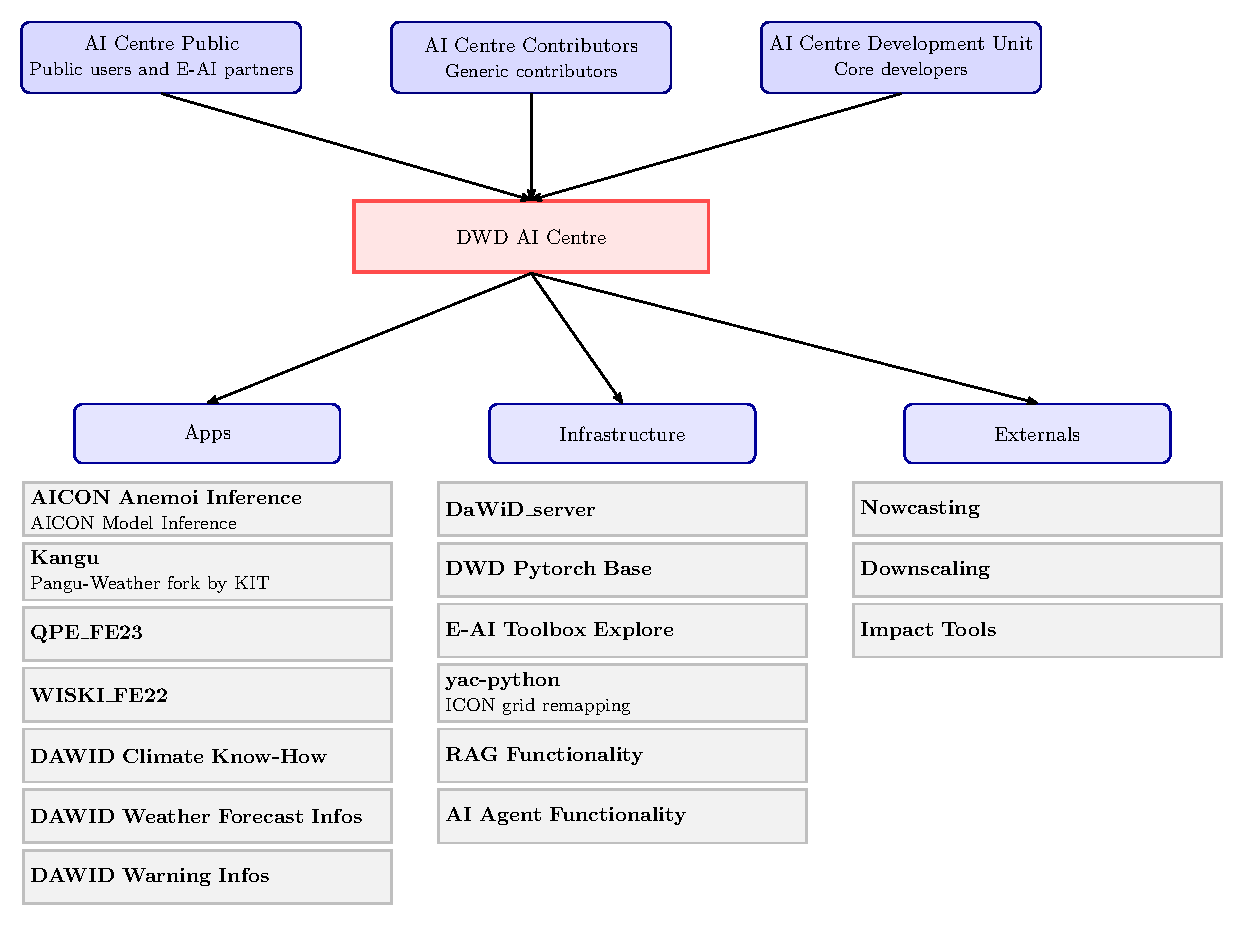
\includegraphics[width=\textwidth]{chapters/ai_centre_graphics.pdf}
  \caption{Organizational and technical structure of the DWD AI Centre repositories.}
  \label{fig:ai_centre_structure}
\end{figure}

\begin{itemize}
  \item The DWD AI Centre connects internal development units, contributors, and public users to shared infrastructure and applications.
  \item The repository structure is grouped into \emph{Apps}, \emph{Infrastructure}, and \emph{Externals}, each containing specific projects for modeling, processing, and integration.
  \item The central node acts as the coordination hub, linking various AI-driven tools with operational workflows and collaborative partners.
\end{itemize}



%==============================================================================
%
%==============================================================================
\section{6 Days Python and AI}

\subsection{Schedule}
\noindent The following table provides an overview of the tutorial structure, covering key topics in Python programming, artificial intelligence, and machine learning for applications in weather, climate, and environmental sciences. The tutorial is designed as a structured six-day course, with each day focusing on a specific theme. The content progresses from fundamental Python concepts and data handling to advanced AI techniques such as large language models (LLMs), retrieval-augmented generation (RAG), and AI-driven forecasting. We introduce many practical applications, and advanced topics including AI data assimilation, model emulation, and AI-enhanced operational workflows. Each day consists of multiple modules, ensuring a comprehensive and hands-on learning experience.

%------------------------------------------------------------------------------
% 
%------------------------------------------------------------------------------
\begin{longtable}{|c|p{5cm}|p{8cm}|}
\hline
\rowcolor{headerblue} \textbf{Chapter} & \textbf{Title} & \textbf{Sections} \\
\hline
\endhead
\hline
\endfoot

%------------------------------------------------------------------------------
\multicolumn{3}{|c|}{\cellcolor{headerblue} \textbf{Day 1: Python as Workhorse}} \\ \hline
\rowcolor{lightblue} 1  & Python Basics & Python syntax, data types, control structures, functions, file I/O \\ \hline
2  & Jupyter Notebooks, APIs and Servers & Setting up Jupyter, working with APIs, creating servers \\ \hline
\rowcolor{lightblue} 3  & Eccodes for Grib, Opendata, NetCDF, Observations, Visualization & GRIB and NetCDF handling with eccodes, accessing OpenData, visualization techniques \\ \hline

%------------------------------------------------------------------------------
\multicolumn{3}{|c|}{\cellcolor{headerblue} \textbf{Day 2: AI/ML Basic Introduction}} \\ \hline
\rowcolor{lightblue} 4  & Machine Learning Basics & Supervised and unsupervised learning, data preprocessing, model evaluation \\ \hline
5  & Neural Network Architectures & Feedforward Networks, Graph Neural Networks, Convolutional Networks, Transformers \\ \hline
\rowcolor{lightblue} 6  & Large Language Models & LLM network structure, Installing and using Ollama, Python API, Local UI with history \\ \hline

%------------------------------------------------------------------------------
\multicolumn{3}{|c|}{\cellcolor{headerblue} \textbf{Day 3: LLM RAG, Python Packages, Multi-Modality}} \\ \hline
\rowcolor{lightblue} 7  & LLM with Retrieval-Augmented Generation (RAG) & Introduction to RAG, Installing dependencies, Loading and processing documents, Generating embeddings, Using FAISS, Retrieving documents, Response generation \\ \hline
8  & Python Packages & Python Standard Library, Xarray basics, Pandas, SciPy, Scikit-learn \\ \hline
\rowcolor{lightblue} 9  & Multimodal LLMs & Modalities, Integration, Fusion, Cross-Attention, Use Cases, AI Interaction, Data Alignment, Benchmarking \\ \hline

%------------------------------------------------------------------------------
\multicolumn{3}{|c|}{\cellcolor{headerblue} \textbf{Day 4: GPUs, AI Agents, Services and Impact}} \\ \hline
\rowcolor{lightblue} 10 & Using GPUs for Training Applications & Checking GPU availability, Installing dependencies, Exploring GPU tensors, Training models on GPU, Comparing CPU vs GPU \\ \hline
11 & Agents and Coding with LLM & Introduction to LLM coding, Agent frameworks, LangChain example, Auto-GPT example \\ \hline
\rowcolor{lightblue} 12 & LLMs for Geosciences, Weather, and Climate & Feature Detection, Weather Reports, Forecast Interpretation, Communication, Impact Forecasting, Decision Support \\ \hline

%------------------------------------------------------------------------------
\multicolumn{3}{|c|}{\cellcolor{headerblue} \textbf{Day 5: LLM Maturity and Operations}} \\ \hline
\rowcolor{lightblue} 13 & MLFlow - Managing and Monitoring Training & Setting up MLFlow, Monitoring Training, Comparing Experiments, Managing Parameters \\ \hline
14 & MLOps - Operations & Principles, Workflow, Deployment, Monitoring, CI/CD, Automation, Reproducibility, Scalability, Kubernetes, Cloud, On-Premise \\ \hline
\rowcolor{lightblue} 15 & Fine-Tuning LLMs & Fine-Tuning, LLMs, Dataset Preparation, Tokenization, LoRA, Reinforcement Learning, Evaluation, Deployment, Scalability \\ \hline

%------------------------------------------------------------------------------
\multicolumn{3}{|c|}{\cellcolor{headerblue} \textbf{Day 6: AI Model and AI Data Assimilation}} \\ \hline
\rowcolor{lightblue} 16 & AnemoI & Overview of AnemoI and its capabilities \\ \hline
17 & Model Emulation and AICON & Emulating weather models with AI, AICON framework \\ \hline
\rowcolor{lightblue} 18 & AI Data Assimilation & AI-driven data assimilation, Applications in numerical weather prediction \\ \hline

%------------------------------------------------------------------------------
% Appendix Section with a Header
%------------------------------------------------------------------------------
\multicolumn{3}{|c|}{\cellcolor{appendixblue} \textbf{Appendix: Background and Additional Topics}} \\ \hline
\rowcolor{lightblue} A1 & Large Language Models - History and Development & History and evolution of LLMs, Key architectures and breakthroughs \\ \hline
A2 & Advanced GPU Utilization & Mixed-precision training, Model parallelism, Efficient GPU scheduling \\ \hline
\rowcolor{lightblue} A3 & Future Trends in AI and Weather Forecasting & Hybrid AI-NWP models, Real-time assimilation, AI-driven extreme event forecasting \\ \hline

\end{longtable}

%==============================================================================
%
%==============================================================================
\subsection{Training Codes}
\noindent To ensure a structured and reproducible learning experience, all training codes are provided \emph{chapter by chapter}. This should allow participants to \emph{easily locate, reference, and execute} the relevant scripts corresponding to specific tutorial sections. 

We have tested the scripts as far as possible for the following computing environments and give specific advice when things were difficult in a particular framework. 

\begin{center}
\begin{figure}[h]
   \centerline{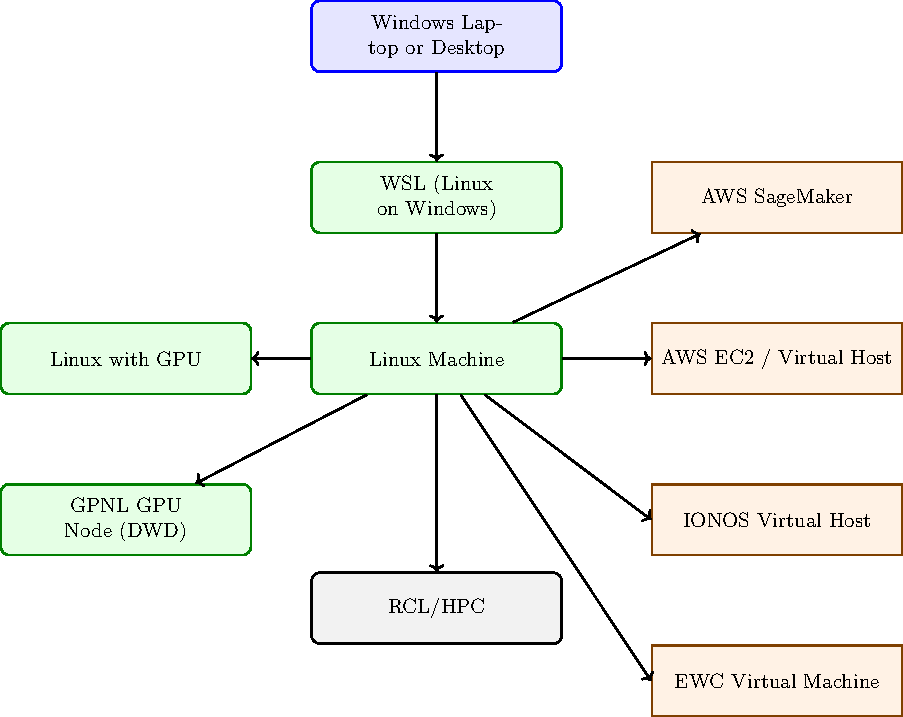
\includegraphics[width=0.8\textwidth]{chapters/computing_environments.pdf}}
	\caption{We want to enable choices and independence of particular solutions or infrastructures.}
\end{figure}
\end{center}%

 % Basic Python, Environments, Modules, Core Language

% Reset numbering after Introduction
\renewcommand{\thechapter}{\arabic{chapter}}
\renewcommand{\thesection}{\arabic{chapter}.\arabic{section}}

%-------------------------------
% Main Matter: Chapters
%-------------------------------
\mainmatter

\addtocontents{toc}{\noindent\hrulefill\vspace{-1.5ex}\par}
\addcontentsline{toc}{chapter}{\textcolor{dwdspecial}{\large Day 1: Python as Workhorse}}

\chapter{Python Basics}

We do not want to provide a full python tutorial, but rather formulate a guide through main steps and a setup which is very flexible to work with python and machine learning for weather, climate and environment. 

Our goal is to enable our scientists and developers to use python and machine learning in a flexible, modular and portable way for their development, for science as well as for products and services of various types. On the basis of python in combination with large language models we will touch the full workflow for science, development, product design and deployment. 

\section{Install, Virtual Environment, Pip und Import}

\subsection{Install and Virtual Environment}
\label{sec:virtualenv}

Before running Python commands, ensure you have Python installed. It is very easy to have Python installed on your laptop by simply downloading it - this is often possible without administration rights. You will then need to set the path variable properly. On Linux, depending on the version installed by your system administrator, you may find the executable under \texttt{python}, \texttt{python3}, \texttt{python3.11} or \texttt{python3.12}. We recommend not working with versions earlier than Python 3.10 because you may run into compatibility issues; instead, make sure you have an up-to-date Python version installed. Test the installed version by:

\begin{codeonly}{Test Python Installation}
python --version 
\end{codeonly}
  
Python has become one of the most popular programming languages, largely because of its extensive ecosystem of packages and libraries. From data analysis and visualization to machine learning and web development, Python's modular design allows you to choose only the components you need.

%------------------------------------------------------------------------------
% Graph Figure
%------------------------------------------------------------------------------
\begin{center}
\begin{tikzpicture}[>=Stealth,
  every node/.style={
    draw, 
    rounded corners, 
    align=center, 
    fill=blue!1, 
    font=\sffamily, 
    inner sep=1mm,
    minimum width=2.5cm, 
    minimum height=1cm
  },
  arrow/.style={-{Stealth[scale=1.2]}, thick}
]
  \matrix (m) [matrix of nodes, row sep=1cm, column sep=1cm, nodes={fill=DWDblue!100,text=white}]{
    & scipy & & \\
    numpy & & pandas & seaborn \\
    & matplotlib & & \\
  };

	\coordinate (via) at ($(m-2-1)!0.7!(m-2-4) + (0,-1)$);

  \draw[arrow] (m-2-1) -- (m-1-2);
  \draw[arrow] (m-2-1) -- (m-3-2);
  \draw[arrow] (m-1-2) -- (m-2-3);
  \draw[arrow] (m-3-2) -- (m-2-3);
  \draw[arrow] (m-2-3) -- (m-2-4);
  \draw[arrow] (m-2-1) -- (via) -- (m-2-4);
	
	\tikzset{
  explanation/.style={
    draw=none,         % No boundary
		fill=none, 
    font=\sffamily\fontseries{ul}\small,  
    align=center       % Centered text
    }
  }
	\tikzset{
  heading/.style={
    draw=none,         % No boundary
		fill=none, 
    font=\sffamily,  
    align=center       % Centered text
    }
  }
\node[heading, above=0mm of m] {\textbf{Package Tree Example}}; % numpy

\node[explanation, above=2mm of m-2-1] {Numerics}; % numpy
\node[explanation, below=2mm of m-1-2] {Scientific \\Computing}; % scipy
\node[explanation, above=2mm of m-3-2] {Visualization}; % scipy
\node[explanation, above=2mm of m-2-3] {Data \\Management}; % pandas
\node[explanation, below=2mm of m-2-4] {Statistical \\Visualization}; % seaborn

\end{tikzpicture}
\end{center}

It is very important to learn to manage packages to build a robust and tailored development environment. Learning how to install, manage, and create packages not only gives you a deeper understanding of the available tools, but also grants you greater control over your projects.

Usually, it is very important for a particular Python environment to provide a complete list of the packages it needs, with their versions, in a consistent framework. This framework is provided by \b1{virtual environments}.

A virtual environment allows you to control your package installations. Below are example commands for both Windows and Linux:

\begin{codeonly}{Windows Command}
python -m venv myenv
myenv\Scripts\activate
\end{codeonly}

\begin{codeonly}{Linux Command}
python3 -m venv myenv
source myenv/bin/activate
\end{codeonly}

This will create a \texttt{myenv} direcotry with the default venv file structure. \texttt{myenv} is the freely choosable name of the venv.  

\subsection{Using \texttt{pip} to Manage Python Packages}

\noindent \texttt{pip} is the package installer for Python. It allows you to install, update, and manage packages from the Python Package Index (PyPI). For example, you can check the version of \texttt{pip}, list installed packages, and install popular packages like \texttt{numpy} and \texttt{matplotlib}. The following commands illustrate these basic operations:

\begin{codeonly}{Basic pip Commands}
pip --version
pip list
pip install numpy
pip install matplotlib
\end{codeonly}

\noindent These commands, when run in your command prompt or terminal, will display the current version of \texttt{pip}, show all installed Python packages, and install \texttt{numpy} and \texttt{matplotlib}, respectively.

One of the most widely used libraries in Python is \texttt{NumPy}, which provides powerful array objects and routines for fast numerical computation. 


%==============================================================================
%
%==============================================================================
\section{Managing Dependencies with \texttt{requirements.txt}}

Managing dependencies is crucial in Python projects, especially when working in different environments or collaborating with others. The \texttt{requirements.txt} file allows you to list all your project’s dependencies and their versions, making it easy to replicate the environment anywhere.

%==============================================================================
%
%==============================================================================
\subsubsection{Generating a \texttt{requirements.txt}}

If you already have a virtual environment set up and want to generate a \texttt{requirements.txt} file from it, first activate your current virtual environment. Once the virtual environment is activated, run the following command to generate the \texttt{requirements.txt} file:

\begin{codeonly}{Generate \texttt{requirements.txt}}
pip freeze > requirements.txt
\end{codeonly}

This creates a file named \texttt{requirements.txt} in your current working directory containing all installed packages and their versions, leading to e.g.\ the following simple requirements.txt file. 

\begin{codeonly}{Requirements.txt}
numpy==1.26.4
ollama==0.3.1
openai==1.69.0
openai-whisper==20240930
toml==0.10.2
torch==2.4.0
torch_geometric==2.5.3
torchmetrics==1.4.1
torchvision==0.19.0
\end{codeonly}

%==============================================================================
%
%==============================================================================
\subsubsection{Installing Dependencies from \texttt{requirements.txt}}

To install all dependencies from an existing \texttt{requirements.txt} file into a new virtual environment, first create and activate the environment as shown in Section~\ref{sec:virtualenv}. Then, run the following command:

\begin{codeonly}{Install Dependencies from \texttt{requirements.txt}}
pip install -r requirements.txt
\end{codeonly}

This installs all packages listed in the \texttt{requirements.txt} file, ensuring that your environment matches the specified dependencies.

With these steps, you can easily share and reproduce Python environments using \texttt{requirements.txt}.

%==============================================================================
%
%==============================================================================
\subsection{Importing Functions or Packages vs. Installation}

In Python, you can either directly import functions and modules from local files or install packages to make them globally available across projects. Understanding the difference is essential for maintaining clean and scalable code.

%==============================================================================
%
%==============================================================================
\subsubsection{Importing Functions or Packages}


You can import Python modules or functions directly from local \texttt{.py} files. For example, if you have the following structure:

\begin{lstlisting}[basicstyle=\ttfamily\small]
|
|-- main_greetings.py
|-- greetings.py
\end{lstlisting}

In \texttt{main\_greetings.py}, you can import from \texttt{greetings.py} as follows:

\begin{codeonly}{main_greetings.py}
# main_greetings.py
from greetings import say_hello

say_hello()
\end{codeonly}

This method is quick and easy for small projects but becomes difficult to manage as your codebase grows or when sharing across multiple projects. You should then create installable packages, we discuss in a moment. 

%==============================================================================
%
%==============================================================================
\subsubsection{The \texttt{importlib} Package in Python}

The \texttt{importlib} package allows you to reload Python modules without restarting the interpreter, which is especially useful during development when modifying code. Normally, Python imports a module only once per session, but \texttt{importlib.reload(module)} forces the interpreter to reload it, reflecting any recent changes. This is particularly handy in interactive environments like Jupyter Notebooks, where you want to see immediate updates after editing a module without restarting the entire session.

\begin{codeonly}{reload\_demo\_fkt.py}
# reload_demo_fkt.py

def greet(name):
    return f"Hello {name}"
\end{codeonly}

And now lets load it, then change the file and reload it. 

\begin{codeonly}{reload\_demo.py}
# reload_demo.py

import importlib
import reload_demo_fkt as mo

def replace_in_file(str1, str2, filename):
    with open(filename, 'r') as file:
        content = file.read()
    content = content.replace(str1, str2)
    with open(filename, 'w') as file:
        file.write(content)

# Call the greet function initially
print(mo.greet("Roland"))  # Expected: Hello Roland

# After modifying reload_demo_fkt.py, reload it
replace_in_file("Hello", "Good Morning", "reload_demo_fkt.py")

importlib.reload(mo)

# Call the updated greet function
print(mo.greet("Roland"))  # Expected: Good Morning Roland

# Restore the original version of the file
replace_in_file("Good Morning", "Hello", "reload_demo_fkt.py")
\end{codeonly}

%==============================================================================
%
%==============================================================================
\subsubsection{Creating an Installable Python Package}


An installable package allows you to reuse and share code easily across different environments. Consider the following structure:

\begin{lstlisting}[basicstyle=\ttfamily\small]
install_demo02/
|-- pyproject.toml
|-- README.md
+-- src/
    +-- install_demo02/
        |-- __init__.py
        |-- install_mod1.py
        |-- install_mod2.py

\end{lstlisting}

The project is defined in a \texttt{pyproject.toml} file, which can include a list of dependencies, that would replace the \texttt{requirements.txt}:

\begin{codeonly}{basic \texttt{pyproject.toml} file}
[build-system]
requires = [ "setuptools>=61"]
build-backend = "setuptools.build_meta"

[project]
name = "install_demo02"   # name of the directory in src/
version = "0.1.3"
description = "A simple Python package with greeting functions"
authors = [
  { name = "Roland Potthast", email = "Roland.Potthast@dwd.de" },
]
requires-python = ">=3.8"
#dependencies = ["numpy<2", "matplotlib",]

[tool.setuptools.packages.find]
where = ["src"]
\end{codeonly}

To install your package locally, in the \texttt{code} folder run:

\begin{codeonly}{Install Your Package}
pip install -e install_demo02/
\end{codeonly}

Once installed, you can import it in any project without reference to the location of the package, as in the file
\texttt{install\_demo\_test\_script.py}: 

\begin{codeonly}{install\_demo\_test\_script.py}
from install_demo02 import greet1, greet2

print(greet1("World"))  # Hello World!
print(greet2("World"))  # Good Morning World!
\end{codeonly}

\textbf{Legacy projects with \texttt{setup.py}}

Before \texttt{pyproject.toml} was invented, packages were defined in a \texttt{setup.py} file.
One can find an example package using \texttt{setup.py} in the \texttt{code/install\_demo} directory.

To make \texttt{setup.py} work on Windows, one might has to use the following steps.
\begin{lstlisting}{}
pip install setuptools wheel
pip install -e install_demo/ --no-build-isolation --no-use-pep517
\end{lstlisting}


%------------------------------------------------------------------------------
%
%------------------------------------------------------------------------------
\noindent \textbf{When to use each approach:}

\begin{itemize}
    \item \emph{Pure Import}: Use for small, single-project code or quick prototypes.
    \item \emph{Installable Package}: Use for larger projects, sharing code, and managing dependencies.
\end{itemize}

%==============================================================================
%
%==============================================================================
\subsubsection{Example: Installing from GitHub}


You can also install packages directly from Git repositories. For example:

\begin{codeonly}{Install from GitHub}
pip install git+https://github.com/username/my_package.git
\end{codeonly}

This installs your package from GitHub, making it easy to share code across teams and projects.

\subsection{What is PyPI?}

The Python Package Index (\textbf{PyPI}) is the official repository for third-party Python packages. It allows developers to:

\begin{itemize}
  \item Upload and share their Python projects with the community.
  \item Install packages using the \texttt{pip} tool.
  \item Manage versions and dependencies of published packages.
\end{itemize}

When a user runs \texttt{pip install some-package}, \texttt{pip} connects to PyPI to find and download the corresponding package.

To make a project available on PyPI, developers package their code (typically using \texttt{pyproject.toml} and tools like \texttt{setuptools} or \texttt{flit}), build the distribution, and upload it using \texttt{twine}.

Uploaded packages are then publicly available for installation and reuse.

For more information, visit the official website:

\href{https://pypi.org}{\texttt{https://pypi.org}}



%==============================================================================
%
%==============================================================================
\section{Introduction to NumPy}

NumPy is the fundamental package for numerical computing in Python. It provides the \texttt{ndarray}, a multidimensional array object that enables fast vectorized operations and efficient handling of large datasets. Although Python is known for its readability, NumPy’s power lies in its ability to perform operations on entire arrays without writing explicit loops—a major benefit for programmers experienced in other languages.

In NumPy, the core building block is the \texttt{ndarray}. An \texttt{ndarray} can be created from a Python list (or nested lists for multidimensional arrays), and it supports element-wise operations. This vectorized computation model is not only more concise but also significantly faster for large-scale computations. Consider the following example:

\begin{codeonly}{Creating Basic Arrays}
import numpy as np
arr1 = np.array([1, 2, 3, 4, 5])
print("1D array:", arr1)
arr2 = np.array([[1, 2, 3], [4, 5, 6]])
print("2D array:")
print(arr2)
\end{codeonly}

The code above shows how to import NumPy (commonly aliased as \texttt{np}) and create both one-dimensional and two-dimensional arrays. Instead of writing loops to process elements, you can use array operations that are both elegant and efficient.

%==============================================================================
%
%==============================================================================
\subsection{Vectorized Operations and Predefined Arrays}

One of NumPy’s most powerful features is vectorized operations. Instead of iterating over each element, you can perform operations on entire arrays with a single expression:

\begin{codeonly}{Vectorized Operations}
import numpy as np
a = np.array([1, 2, 3, 4, 5])
b = np.array([10, 20, 30, 40, 50])
c = a + b
d = a * b
print("Addition:", c)
print("Multiplication:", d)
\end{codeonly}

In addition to these operations, NumPy offers a variety of functions for creating arrays with predefined values. This is useful for initializing data or generating test datasets:

\begin{codeonly}{Predefined Arrays}
import numpy as np
zeros = np.zeros((3, 4))
print("Zeros array:")
print(zeros)
ones = np.ones((2, 5))
print("Ones array:")
print(ones)
range_array = np.arange(0, 10, 2)
print("Range array:", range_array)
linspace_array = np.linspace(0, 1, 5)
print("Linspace array:", linspace_array)
\end{codeonly}

%==============================================================================
%
%==============================================================================
\subsection{Slicing, Indexing, and Broadcasting}

NumPy arrays support powerful slicing and indexing methods, similar to Python lists but extended to multiple dimensions. This feature allows you to extract subarrays efficiently without copying the data:

\begin{codeonly}{Slicing and Indexing}
import numpy as np
matrix = np.array([[ 1,  2,  3,  4],
                   [ 5,  6,  7,  8],
                   [ 9, 10, 11, 12],
                   [13, 14, 15, 16]])
submatrix = matrix[1:4, 1:4]
print("Submatrix:")
print(submatrix)
element = matrix[1, 2]
print("Element at (2,3):", element)
\end{codeonly}

Broadcasting allows operations between arrays of different shapes. With broadcasting, NumPy automatically expands the dimensions of an array during arithmetic operations:

\begin{codeonly}{Broadcasting Example}
import numpy as np
mat = np.array([[1, 2, 3],
                [4, 5, 6],
                [7, 8, 9]])
vec = np.array([1, 0, -1])
result = mat - vec
print("Broadcasting result:")
print(result)
\end{codeonly}

%==============================================================================
%
%==============================================================================
\subsection{Mathematical Functions and Applications}

NumPy offers a comprehensive suite of mathematical functions that operate element-wise on arrays. Whether you need trigonometric, logarithmic, or exponential functions, NumPy has you covered:

\begin{codeonly}{Mathematical Functions}
import numpy as np
angles = np.linspace(0, np.pi, 5)
print("Angles:", angles)
sine_values = np.sin(angles)
print("Sine values:", sine_values)
exp_values = np.exp(np.array([0, 1, 2]))
print("Exponential values:", exp_values)
\end{codeonly}

Using these functions, you can perform complex numerical computations with minimal code. For example, you might model a physical phenomenon or simulate data; NumPy’s capabilities allow you to transform and analyze data efficiently Experiment with these examples, and explore further functionalities of NumPy to fully leverage Python's capabilities in scientific computing.

\begin{recommendationbox}
Make sure you know your basic python commands well! Initially, do not rely only on sophisticated packages. Keep the core python level as your active knowledge!
\end{recommendationbox}

%==============================================================================
%
%==============================================================================
\section{Generating Plots based on Matplotlib}

Paired with \texttt{Matplotlib}, a versatile plotting library, you can quickly visualize data and test your ideas. 

%==============================================================================
%
%==============================================================================
\subsection{1D Plots}
The following example demonstrates how to use these libraries to plot a simple curve. In this code snippet, we generate a sine wave using \texttt{NumPy} and then plot it with \texttt{Matplotlib}.

\begin{codeonly}{plot-sine-wave.py}
import numpy as np
import matplotlib.pyplot as plt

# Generate data
x = np.linspace(0, 10, 100)
y = np.sin(x)

# Create the plot
plt.figure(figsize=(4, 3))
plt.plot(x, y)
plt.xlabel('x')
plt.ylabel('sin(x)')
plt.title('Image generated by Simple Python Code')

# Save the plot as a PNG file
plt.savefig('images/plot-sine-wave.png')
plt.close()  # Close the figure to free up memory
\end{codeonly}

\begin{center}
   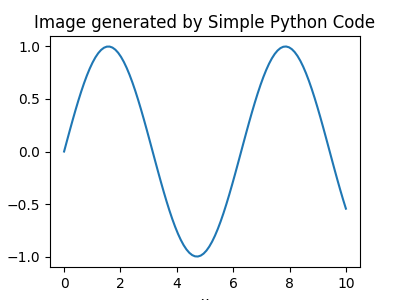
\includegraphics[width=0.6\textwidth]{images/plot-sine-wave.png}
\end{center}%

%==============================================================================
%
%==============================================================================
\subsection{2D Plots}

The following code demonstrates how to generate and visualize a two-dimensional field using NumPy and Matplotlib. First, a symmetric grid of x and y values is created and the radial distance from the origin is computed. Then, a Gaussian-modulated cosine function is used to define a smoothly varying field that decays with distance from the center. Finally, a filled contour plot is generated to visualize the field, and the resulting image is saved as a PNG file.

\begin{codeonly}{plot-gaussian-modulated-cosine-field.py}
import numpy as np
import matplotlib.pyplot as plt

# Create a grid of x and y values (centered at 0 for a symmetric field)
x = np.linspace(-10, 10, 200)
y = np.linspace(-10, 10, 200)
X, Y = np.meshgrid(x, y)

# Compute the radial distance from the origin
R = np.sqrt(X**2 + Y**2)

# Define a Gaussian-modulated cosine field
Z = np.exp(-0.1*(X**2 + Y**2)) * np.cos(5*R)

# Create a filled contour plot for the 2D field
plt.figure(figsize=(4, 3))
contour = plt.contourf(X, Y, Z, levels=50, cmap='viridis')
plt.colorbar(contour, label='Field value')
plt.xlabel('X')
plt.ylabel('Y')
plt.title('2D Field Plot: Gaussian-Modulated Cosine')
plt.savefig('images/plot-gaussian-modulated-cosine-field.png')
plt.close()
\end{codeonly}

\begin{center}
   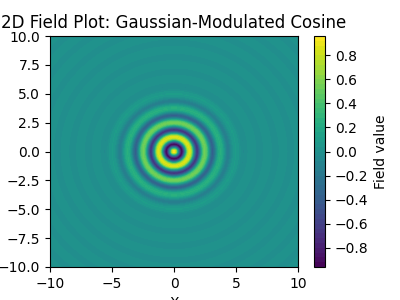
\includegraphics[width=0.6\textwidth]{images/plot-gaussian-modulated-cosine-field.png}
\end{center}%

The next example demonstrates how to create a simple 3D surface plot using Matplotlib's built-in \texttt{mplot3d} toolkit. By generating a meshgrid of \(x\) and \(y\) values and computing a corresponding \(z\) value from a radial sine function, the plot visualizes a three-dimensional wave-like pattern. This technique provides a straightforward way to represent and explore three-dimensional data in Python.

\begin{codeonly}{}

\end{codeonly}

\begin{center}
   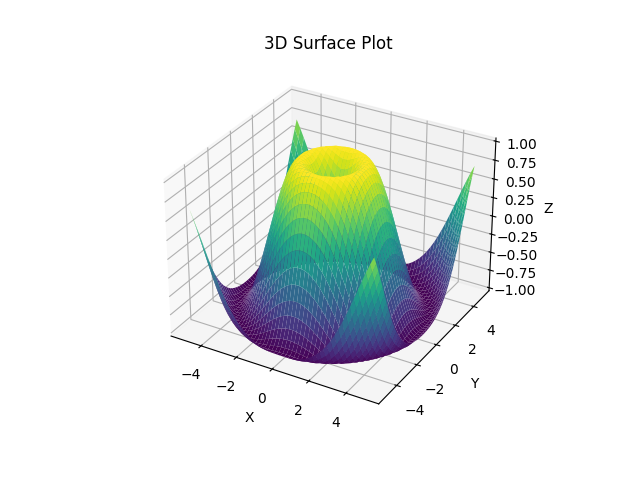
\includegraphics[width=0.6\textwidth]{images/plot-3d-surface.png}
\end{center}%

%==============================================================================
%
%==============================================================================
\section{Functions}

Python functions are reusable blocks of code that allow you to encapsulate logic and perform specific tasks. In Python, functions are defined using the \texttt{def} keyword and can take parameters, return values, and include documentation. The following sections introduce the basics of defining and using functions in Python.

%==============================================================================
%
%==============================================================================
\subsection{Defining a Function}
Functions are defined with the \texttt{def} keyword followed by the function name, parentheses containing any parameters, and a colon. The function body is indented. Here is a basic example that defines a function to greet a user:

\begin{codeonly}{Defining a Function}
def greet(name):
    """Return a greeting message."""
    return f"Hello, {name}!"
\end{codeonly}

%==============================================================================
%
%==============================================================================
\subsection{Calling a Function}
Once a function is defined, you can call it by using its name followed by parentheses containing any required arguments. The following example shows how to call the \texttt{greet} function and print its result:

\begin{codeonly}{Calling a Function}
message = greet("Alice")
print(message)
\end{codeonly}

%==============================================================================
%
%==============================================================================
\subsection{Functions with Multiple Parameters}
A function can accept multiple parameters. Below is an example of a function that calculates the area of a rectangle:

\begin{codeonly}{Function with Multiple Parameters}
def rectangle_area(width, height):
    """Calculate the area of a rectangle."""
    return width * height

area = rectangle_area(5, 3)
print("The area of the rectangle is:", area)
\end{codeonly}

%==============================================================================
%
%==============================================================================
\subsection{Default Parameter Values}
Python functions can have default parameter values, which are used when an argument is not provided. This example demonstrates a function that computes a power, using a default exponent of 2:

\begin{codeonly}{Default Parameter Values}
def power(number, exponent=2):
    """Return number raised to the power of exponent."""
    return number ** exponent

print(power(4))    # Uses default exponent 2 (result: 16)
print(power(2, 3)) # Exponent explicitly set to 3 (result: 8)
\end{codeonly}

%==============================================================================
%
%==============================================================================
\subsubsection{Variable-Length Arguments}
Sometimes, you may not know in advance how many arguments a function should accept. Python allows you to capture additional positional arguments using the \texttt{*args} syntax. In the following example, a function computes the sum of an arbitrary number of numbers:

\begin{codeonly}{Variable-Length Arguments}
def total_sum(*args):
    """Return the sum of all provided arguments."""
    return sum(args)

print(total_sum(1, 2, 3, 4, 5))  # Output: 15
\end{codeonly}


%==============================================================================
%
%==============================================================================
\section{Python Essentials}

Let us look at a survey table what basic python knowledge you should gain in a first step. 
We have already gone over some sigificant part of this, and will briefly give you a head-start for
the remaining points. 

\begin{table}[h!]
\centering
\begin{tabular}{|p{4cm}|p{8cm}|}
\hline
\textbf{Topic} & \textbf{Description} \\ \hline
Python Syntax & Basic structure, indentation, comments \\ \hline
Data Types & Integers, floats, strings, booleans, lists, tuples, sets, dictionaries \\ \hline
Control Flow & \texttt{if-else}, \texttt{for} and \texttt{while} loops, \texttt{break}, \texttt{continue} \\ \hline
Functions & Defining functions with \texttt{def}, arguments, return values, lambda functions \\ \hline
Modules and Imports & Importing built-in and external libraries, creating custom modules \\ \hline
File I/O & Reading and writing files, using \texttt{with} statements \\ \hline
Exception Handling & Using \texttt{try-except} for error handling \\ \hline
Object-Oriented Programming (OOP) & Classes, objects, inheritance, and polymorphism \\ \hline
Standard Libraries & Common libraries like \texttt{os}, \texttt{sys}, \texttt{math}, \texttt{datetime}, \texttt{json} \\ \hline
Virtual Environments & Creating and managing virtual environments with \texttt{venv} or \texttt{conda} \\ \hline
\end{tabular}
\caption{Essential Topics for Basic Python Learning}
\label{tab:basic_python_topics}
\end{table}

%==============================================================================
%
%==============================================================================
\subsection{Control Flow in Python}

Control flow in Python refers to the order in which individual statements, instructions, or function calls are executed. Python provides several structures for controlling the flow of your program, including conditionals, loops, and exception handling.

%==============================================================================
%
%==============================================================================
\subsubsection{Conditional Statements}

Conditional statements allow you to execute different code blocks based on certain conditions.

\textbf{Example:}
\begin{codeonly}{If-Else Statements}
x = 10
if x > 0:
    print("Positive")
elif x == 0:
    print("Zero")
else:
    print("Negative")
\end{codeonly}

%==============================================================================
%
%==============================================================================
\subsubsection{Loops}

Loops allow you to repeat a block of code multiple times.

\textbf{For Loop Example:}
\begin{codeonly}{For Loop}
for i in range(5):
    print(i)
\end{codeonly}

\textbf{While Loop Example:}
\begin{codeonly}{While Loop}
count = 0
while count < 5:
    print(count)
    count += 1
\end{codeonly}

%==============================================================================
%
%==============================================================================
\subsubsection{Loop Control Statements}

Python provides special statements to control the flow inside loops:
\begin{itemize}
    \item \texttt{break} – Exits the loop prematurely.
    \item \texttt{continue} – Skips the rest of the current iteration.
    \item \texttt{pass} – Does nothing and acts as a placeholder.
\end{itemize}

\textbf{Example with \texttt{break} and \texttt{continue}:}
\begin{codeonly}{Loop Control Example}
for i in range(10):
    if i == 3:
        continue  # Skip 3
    if i == 7:
        break  # Stop loop at 7
    print(i)
\end{codeonly}

%==============================================================================
%
%==============================================================================
\subsubsection{Exception Handling}

Python allows you to handle errors using \texttt{try-except} blocks to prevent program crashes.

\textbf{Example:}
\begin{codeonly}{Try-Except Block}
try:
    result = 10 / 0
except ZeroDivisionError:
    print("Cannot divide by zero!")
\end{codeonly}

\textbf{Summary:} Control flow structures are essential for building logical and efficient Python programs, allowing you to make decisions, iterate over data, and handle errors gracefully.


%==============================================================================
%
%==============================================================================
\subsection{File Input and Output in Python}

Python provides built-in functions to handle files, making it easy to read from and write to files. This section covers the basics of File I/O operations.

%==============================================================================
%
%==============================================================================
\subsubsection{Opening and Closing Files}

To work with files, you need to open them first using the \texttt{open()} function and close them when done using \texttt{close()}.

\textbf{Example:}
\begin{codeonly}{Open and Close a File}
file = open('example.txt', 'r')  # Open in read mode
content = file.read()  # Read the file content
file.close()  # Close the file
\end{codeonly}

%==============================================================================
%
%==============================================================================
\subsubsection{Reading from Files}

Python provides multiple methods to read file content:
\begin{itemize}
    \item \texttt{read()} – Reads the entire file.
    \item \texttt{readline()} – Reads one line at a time.
    \item \texttt{readlines()} – Reads all lines into a list.
\end{itemize}

\textbf{Example:}
\begin{codeonly}{Reading from a File}
with open('example.txt', 'r') as file:
    for line in file:
        print(line.strip())
\end{codeonly}

%==============================================================================
%
%==============================================================================
\subsubsection{Writing to Files}

To write to a file, open it in write mode (\texttt{'w'}) or append mode (\texttt{'a'}).

\textbf{Example:}
\begin{codeonly}{Writing to a File}
with open('output.txt', 'w') as file:
    file.write('Hello, Python!\n')
    file.write('This is a new line.')
\end{codeonly}

%==============================================================================
%
%==============================================================================
\subsubsection{File Modes in Python}

\begin{itemize}
    \item \texttt{'r'} – Read mode (default).
    \item \texttt{'w'} – Write mode (overwrites file).
    \item \texttt{'a'} – Append mode.
    \item \texttt{'rb'} – Read binary mode.
    \item \texttt{'wb'} – Write binary mode.
\end{itemize}

%==============================================================================
%
%==============================================================================
\subsubsection{Using the \texttt{with} Statement}

The \texttt{with} statement simplifies file handling by automatically closing the file when the block is done.

\textbf{Example:}
\begin{codeonly}{Using the with Statement}
with open('data.txt', 'r') as file:
    data = file.read()
    print(data)
\end{codeonly}

\textbf{Summary:} File I/O in Python is straightforward and efficient, with built-in methods that handle files securely and reliably.

%==============================================================================
%
%==============================================================================
\subsection{Common Python Libraries: \texttt{os}, \texttt{sys}, \texttt{math}, \texttt{datetime}, and \texttt{json}}

Python’s standard library provides a rich set of modules for everyday tasks. This section covers some of the most commonly used libraries.

%==============================================================================
%
%==============================================================================
\subsubsection{\texttt{os} – Operating System Interface}

The \texttt{os} module provides functions for interacting with the operating system, such as handling files, directories, and environment variables.

\textbf{Example:}
\begin{codeonly}{Using the os Module}
import os

print(os.getcwd())  # Get current working directory
os.mkdir('new_folder')  # Create a new folder
os.remove('file.txt')  # Delete a file
\end{codeonly}

%==============================================================================
%
%==============================================================================
\subsubsection{\texttt{sys} – System-Specific Parameters}

The \texttt{sys} module provides access to system-specific parameters and functions, such as command-line arguments and exiting the program.

\textbf{Example:}
\begin{codeonly}{Using the sys Module}
import sys

print(sys.argv)  # Command-line arguments
sys.exit(0)  # Exit the program
\end{codeonly}

%==============================================================================
%
%==============================================================================
\subsubsection{\texttt{math} – Mathematical Functions}

The \texttt{math} module offers mathematical functions such as trigonometry, logarithms, and factorials.

\textbf{Example:}
\begin{codeonly}{Using the math Module}
import math

print(math.sqrt(16))  # Square root
print(math.pi)  # Value of pi
print(math.factorial(5))  # Factorial of 5
\end{codeonly}

%==============================================================================
%
%==============================================================================
\subsubsection{\texttt{datetime} – Working with Dates and Times}

The \texttt{datetime} module provides classes for working with dates and times, including formatting and arithmetic operations.

\textbf{Example:}
\begin{codeonly}{Using the datetime Module}
from datetime import datetime

now = datetime.now()
print(now.strftime("%Y-%m-%d %H:%M:%S"))  # Format current date and time
\end{codeonly}

%==============================================================================
%
%==============================================================================
\subsubsection{Dictionaries – Key-Value Data Structures}

A \texttt{dict} in Python is an unordered collection of key-value pairs. Each key must be unique and immutable, and it maps to a corresponding value.

\textbf{Example:}
\begin{codeonly}{Using a Python Dictionary}
data = {'name': 'Alice', 'age': 30}

print(data['name'])     # Access value by key
data['age'] = 31        # Update value
data['city'] = 'Paris'  # Add new key-value pair

print(data)
\end{codeonly}

\textbf{Summary:} Dictionaries are a powerful and flexible way to store structured data, enabling quick access and modification using keys. They are one of Python's most important built-in data types.

%==============================================================================
%
%==============================================================================
\subsubsection{\texttt{json} – JSON Data Handling}

The \texttt{json} module allows you to parse JSON data from strings or files and convert Python objects to JSON format.

\textbf{Example:}
\begin{codeonly}{Using the json Module}
import json

data = {'name': 'Alice', 'age': 30}
json_string = json.dumps(data)  # Convert to JSON string
print(json.loads(json_string))  # Convert JSON string to Python object
\end{codeonly}

\textbf{Summary:} These libraries provide essential functions for system interaction, mathematical computations, date/time manipulation, and data serialization, making them fundamental for Python development.

%==============================================================================
%
%==============================================================================
\subsection{Python Classes: Earth System Modeling Example}

To demonstrate object-oriented programming in a scientific context, we implement a simple Earth System Model in Python. This example shows how classes can structure complex models by representing different components of the Earth system.

%==============================================================================
%
%==============================================================================
\subsubsection{Defining Earth System Components}

We create a base class \texttt{EarthSystemComponent} and extend it for each component like \texttt{Atmosphere}, \texttt{Ocean}, and \texttt{Land}. This can be found in \texttt{code-ch01-sec06-earth-system-simulation.py}.

\begin{codeonly}{Defining Earth System Components}
class EarthSystemComponent:
    def __init__(self, name):
        self.name = name

    def simulate(self):
        raise NotImplementedError("This method should be implemented by subclasses")

class Atmosphere(EarthSystemComponent):
    def simulate(self):
        return f"Simulating {self.name}: Temperature, pressure, and wind patterns"

class Ocean(EarthSystemComponent):
    def simulate(self):
        return f"Simulating {self.name}: Currents, salinity, and sea surface temperatures"

class Land(EarthSystemComponent):
    def simulate(self):
        return f"Simulating {self.name}: Soil moisture, vegetation, and surface temperature"
\end{codeonly}

%==============================================================================
%
%==============================================================================
\subsubsection{Building the Earth System Model}

A main class \texttt{EarthSystemModel} is created to manage all components and run the simulation.

\begin{codeonly}{Earth System Model Class}
class EarthSystemModel:
    def __init__(self):
        self.components = []

    def add_component(self, component):
        self.components.append(component)

    def run_simulation(self):
        for component in self.components:
            print(component.simulate())
\end{codeonly}

%==============================================================================
%
%==============================================================================
\subsubsection{Running the Simulation}

We instantiate the components, add them to the model, and run the simulation:

\begin{codeonly}{Running the Earth System Simulation}
atmosphere = Atmosphere("Global Atmosphere")
ocean = Ocean("Global Ocean")
land = Land("Global Land")

model = EarthSystemModel()
model.add_component(atmosphere)
model.add_component(ocean)
model.add_component(land)

model.run_simulation()
\end{codeonly}

\textbf{Output:}
\begin{verbatim}
Simulating Global Atmosphere: Temperature, pressure, and wind patterns
Simulating Global Ocean: Currents, salinity, and sea surface temperatures
Simulating Global Land: Soil moisture, vegetation, and surface temperature
\end{verbatim}

This example showcases the power of OOP for complex systems, providing modularity, reusability, and clear organization in scientific models.

 % Basic Python, Environments, Modules, Core Language
\chapter{Jupyter Notebooks, APIs and Servers}

%==============================================================================
%
%==============================================================================
\section{Introduction to Jupyter Notebooks}

%==============================================================================
%
%==============================================================================
\subsection{What is Jupyter Notebook?}


Jupyter Notebook is an open-source web-based tool that allows you to create and share documents containing live code, equations, visualizations, and explanatory text. It supports various programming languages, including Python, making it an essential tool for data analysis, machine learning, and scientific computing. Its interactive nature allows for rapid prototyping, testing, and visualization of code, making it particularly useful for beginners and experts alike.

%==============================================================================
%
%==============================================================================
\subsection{Installing and Running Jupyter}

To install Jupyter Notebook, use Python’s package manager, \texttt{pip}:

\begin{codeonly}{Install Jupyter Notebook}
pip install jupyter
pip install jupysterlab
\end{codeonly}

Once installed, you can start Jupyter Notebook by running the following command in your terminal:

\begin{codeonly}{Run Jupyter Notebook}
jupyter notebook
\end{codeonly}

or \texttt{jupyter notebook mynotebook.ipynb}. This will open a web browser with the Jupyter interface, allowing you to create and manage notebooks. On many clouds there is jupyter pre-installed with many packages which you might want to use. 

As an example, Amazon Web Services (AWS) for example offers a ready-to-go machine learning framework where you get all packages for using pytorch from the beginning. However, running any of these will cost you per hour - do not forget to shut it down once you are done, otherwise you might be surprised how small amounts of payments can accumulate over days and weeks (happened to me once). 

%==============================================================================
%
%==============================================================================
\subsection{Basic Operations in Jupyter}

In Jupyter, each notebook consists of cells that can hold code, text, or markdown. Common operations include:

\begin{itemize}
    \item \bbb{Running Code:} Press \texttt{Shift+Enter} to execute the code in the current cell and move to the next.
    \item \bbb{Adding Cells:} Use the \texttt{+} button or press \texttt{B} to add a cell below the current one.
    \item \bbb{Changing Cell Type:} Switch between \texttt{Code} and \texttt{Markdown} using the dropdown or press \texttt{Esc + M}.
    \item \bbb{Saving Notebooks:} Press \texttt{Ctrl+S} or use the \texttt{Save} button to save your work.
		\item \bbb{Export as Code:} You can export a Jupyter Notebook to a Python code file by selecting \texttt{File > Download as > Python (.py)} in the Jupyter interface, or by running the command \texttt{jupyter nbconvert --to script notebook.ipynb} in the terminal.
\end{itemize}

Jupyter also provides built-in visualization support with libraries like \texttt{matplotlib}, making it ideal for data-driven projects. Its flexibility and ease of use make it a crucial tool for Python developers.

%==============================================================================
%
%==============================================================================
\subsection{Installing Packages in Jupyter Notebooks with \texttt{!pip install}}

In Jupyter Notebooks, you can install Python packages directly from within a code cell using the exclamation mark (\texttt{!}) followed by the usual \texttt{pip install} command. This is particularly useful because it eliminates the need to switch to a terminal or command line interface. The packages go into the virtual environment you have been using to call jupyter. 

To install a package, simply run:

\begin{codeonly}{Installing a Package in Jupyter}
!pip install numpy
\end{codeonly}

This command installs the \texttt{numpy} package in your current Jupyter environment.

\textbf{Why use \texttt{!pip install} in Jupyter?}
\begin{itemize}
    \item It ensures that the package is installed directly into the environment where the notebook is running.
    \item Convenient for interactive development without leaving the notebook interface.
\end{itemize}

If you encounter issues where Jupyter uses a different Python environment than your terminal, you can explicitly install packages to the notebook's Python environment by using:

\begin{codeonly}{Ensuring Correct Environment}
import sys
!{sys.executable} -m pip install package_name
\end{codeonly}

where
\begin{lstlisting}
print({sys.executable})
\end{lstlisting}
shows the path of the current python binary used for execution, i.e.

\begin{lstlisting}
{'C:\\Users\\rolan\\all\\ropy312\\Scripts\\python.exe'}
\end{lstlisting}
on my windows computer. 

This guarantees that \texttt{pip} installs the package into the environment running the notebook, ensuring compatibility and avoiding common environment issues.

%==============================================================================
%
%==============================================================================
\subsection{Running Jupyter on a Remote Linux Machine with Port Forwarding}

When working on remote servers, such as a Linux machine over SSH, you can still use Jupyter Notebooks by starting it on the remote machine and forwarding the port to your local machine (Windows or Linux). This ensures you can access the notebook in your local browser while running the code on the powerful remote server.

\subsubsection{Starting Jupyter on the Remote Linux Machine}

First, log in to your remote Linux machine via SSH. Then, start Jupyter Notebook with:
\begin{codeonly}{Remote Command on Linux}
jupyter notebook --no-browser --port=8888
\end{codeonly}

This command starts Jupyter on port \texttt{8888} without opening a browser window on the remote machine.

\subsubsection{Port Forwarding from Local Machine}

To access this remote Jupyter server, you need to forward the port from the remote machine to your local machine.
On a local Linux machine (using Bash) or Windows (Powershell):
\begin{codeonly}{Port Forwarding on Linux}
ssh -N -L 9001:localhost:8888 user@remote-server-ip &
\end{codeonly}

This forwards the remote port \texttt{8888} to your local machine’s port \texttt{9001}.


\subsubsection{Accessing Jupyter Notebook in Your Local Browser}

Once the SSH connection is established, open a browser on your local machine and navigate to:
\begin{verbatim}
http://localhost:9001
\end{verbatim}

You will see the Jupyter Notebook interface running on the remote machine, accessible from your local browser. However, it will probably ask you for the token, which is displayed when you start the Jupyter notebook: 

\begin{lstlisting}
    To access the server, open this file in a browser:
        file:///home/roland/.local/share/jupyter/runtime/jpserver-6745-open.html
    Or copy and paste one of these URLs:
        http://localhost:8888/tree?token=2bfafead00bd642b4fc56a57864e3e9ca92bc41e49f4c1f6
        http://127.0.0.1:8888/tree?token=2bfafead00bd642b4fc56a57864e3e9ca92bc41e49f4c1f6
\end{lstlisting}

The port 8888, however, is on the remote machine, you have forwarded it locally to 9001 and need to replace this, then use your browser to access the Jupyter notebook. 

%==============================================================================
%
%==============================================================================
\subsection{Using Markdown Cells for Documentation}

Markdown cells in Jupyter Notebooks allow you to add formatted text, making your notebooks more readable and well-documented. To create a Markdown cell, simply change the cell type from \texttt{Code} to \texttt{Markdown}.

Markdown supports:
\begin{itemize}
    \item \bbb{Headings:} Use \texttt{\#} for headings (\texttt{\# Heading 1}, \texttt{\#\# Heading 2}).
    \item \bbb{Bold and Italics:} Use \texttt{**bold**} or \texttt{*italic*}.
    \item \bbb{Lists:} Create ordered lists with numbers and unordered lists with dashes.
    \item \bbb{Links and Images:} Add links with \texttt{[text](url)} and images with \texttt{![alt text](image\_url)}.
    \item \bbb{LaTeX Equations:} For mathematical expressions, enclose LaTeX code in \texttt{\$...\$} for inline equations or \texttt{\$\$...\$\$} for display equations.
\end{itemize}

Markdown transforms Jupyter notebooks into interactive documents combining code, text, and visuals seamlessly.

%==============================================================================
%
%==============================================================================
\subsection{Using Magic Commands in Jupyter Notebooks}

Jupyter provides special \bbb{magic commands} that simplify various tasks such as timing code execution, managing the environment, and more. Magic commands start with a single \texttt{\%} for line magics and \texttt{\%\%} for cell magics.

\textbf{Common Magic Commands:}
\begin{itemize}
    \item \texttt{\%time}: Times the execution of a single line of code.
    \begin{codeonly}{Timing a Code Line}
%time sum(range(1000000))
    \end{codeonly}
    \item \texttt{\%timeit}: Runs code multiple times and gives an average runtime.
    \item \texttt{\%lsmagic}: Lists all available magic commands.
    \item \texttt{\%\%writefile}: Writes the contents of a cell to an external file.
\begin{codeonly}{Writing to a File}
%%writefile magic_hello.py
print("Hello, world!")
\end{codeonly}
    \item \texttt{\%\%bash}: Runs Bash commands directly inside a Jupyter cell.
\end{itemize}

Magic commands enhance productivity by providing quick, built-in operations within Jupyter.

%==============================================================================
%
%==============================================================================
\subsection{Running Shell Commands in Jupyter Notebooks}

Jupyter allows you to execute shell commands directly within code cells using the exclamation mark (\texttt{!}). This is useful for interacting with the operating system without leaving the notebook.

\textbf{Examples of Shell Commands in Jupyter:}
\begin{itemize}
    \item List files in the current directory:
    \begin{codeonly}{List Files}
!ls
    \end{codeonly}
    \item Install packages using \texttt{pip}:
    \begin{codeonly}{Install a Package}
!pip install numpy
    \end{codeonly}
    \item Check the Python version:
    \begin{codeonly}{Check Python Version}
!python --version
    \end{codeonly}
\end{itemize}

Shell commands allow seamless interaction with the system, making Jupyter highly versatile for both coding and administrative tasks.

%==============================================================================
%
%==============================================================================
\subsection{Data Visualization in Jupyter with Matplotlib, Seaborn, and Plotly}

Jupyter Notebooks integrate well with popular Python visualization libraries, making it easy to create plots and graphs directly within your notebook.

\begin{codeonly}{Lorenz63 Calculation and Visualization}
import numpy as np
import matplotlib.pyplot as plt

# Parameters and initial condition
sigma, beta, rho = 10, 8/3, 28
dt, steps = 0.01, 10000
xyz = np.empty((steps, 3))
xyz[0] = (1, 1, 1)

# Integration using Euler method
for i in range(steps - 1):
    x, y, z = xyz[i]
    dx = sigma * (y - x)
    dy = x * (rho - z) - y
    dz = x * y - beta * z
    xyz[i + 1] = xyz[i] + dt * np.array([dx, dy, dz])

# Plot the result
fig = plt.figure(figsize=(6, 4))
ax = fig.add_subplot(projection='3d')
ax.plot(*xyz.T, lw=0.5)
ax.set_title("Lorenz Attractor")
ax.set_facecolor("white")       # plot area (axes background)
plt.savefig('images/lorenz63.png')
plt.show()
\end{codeonly}

\begin{center}
\begin{figure}[ht]
   \centerline{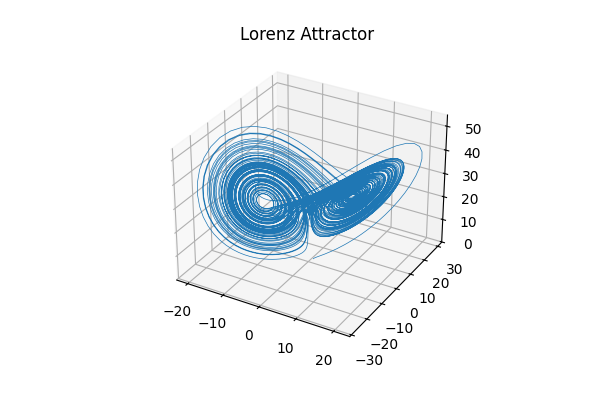
\includegraphics[width=0.8\textwidth]{images/lorenz63.png}}
	 \caption{Matplotlib within Jupyter, Lorenz 63 Attractor.}
\end{figure}
\end{center}%

And another code based on the seaborne package, where you need to \texttt{pip install seaborn} first, then run: 

\begin{codeonly}{lorenz63-seaborn.py}
import numpy as np
import matplotlib.pyplot as plt
import seaborn as sns

# Parameters for the Lorenz system
s = 10.0   # Sigma
r = 28.0   # Rho
b = 8.0 / 3.0  # Beta

# Time step and number of iterations
dt, N = 0.01, 10000

# Array to hold x, y, z
xyz = np.zeros((N, 3))
xyz[0] = 1, 1, 1  # Initial condition

# Integrate using Euler's method
for i in range(1, N):
    x, y, z = xyz[i-1]
    dx = s * (y - x)
    dy = x * (r - z) - y
    dz = x * y - b * z
    xyz[i] = x + dt * dx, y + dt * dy, z + dt * dz

# KDE plot with seaborn
sns.set(style="white")
plt.figure(figsize=(6, 5))
kde = sns.kdeplot(
    x=xyz[:, 0], y=xyz[:, 2],  # x vs z
    fill=True, cmap="viridis", levels=100, thresh=0.02
)
plt.colorbar(kde.collections[0], label="Density")
plt.title("Lorenz Attractor Density (x vs z)")
plt.xlabel("x")
plt.ylabel("z")
plt.tight_layout()
plt.savefig("images/lorenz63-seaborn.png")
plt.show()
\end{codeonly}

\begin{center}
\begin{figure}[ht]
   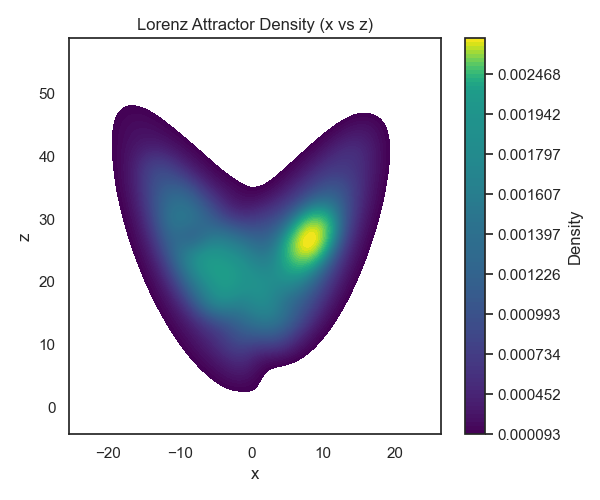
\includegraphics[width=0.35\textwidth]{images/lorenz63-seaborn.png}
   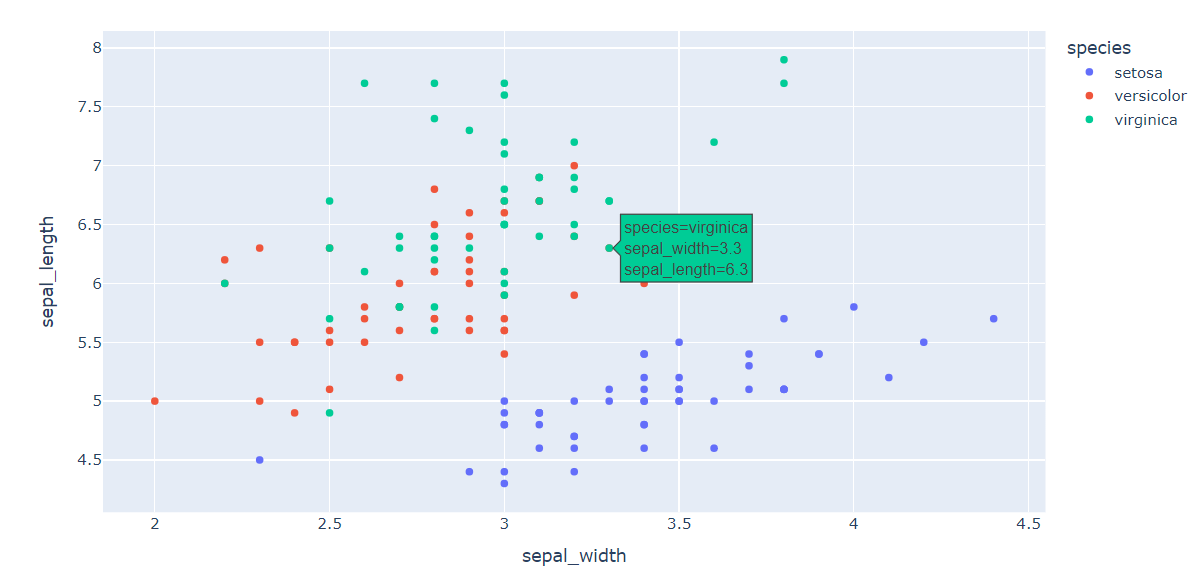
\includegraphics[width=0.6\textwidth]{images/plotly_interactive.png}
	\caption{Density visualization based on seaborne package and interactive plotly visualization.}
\end{figure}
\end{center}%

Interactive plots can easily be integrated into jupyter notebooks, here for example with the \emph{plotly} package. You need to install
\begin{lstlisting}
pip install numpy
pip install plotly
pip install pandas
\end{lstlisting}
We will discuss pandas further in a later session. 

\textbf{Using \texttt{plotly} for Interactive Plots:}
\begin{codeonly}{Plotly Example}
import plotly.express as px
df = px.data.iris()
fig = px.scatter(df, x='sepal_width', y='sepal_length', color='species')
fig.show()
\end{codeonly}

With these and further libraries, Jupyter becomes a powerful tool for both static and interactive data visualizations. You cannot develop applications in artificial intelligence without looking at data and results in a very careful way, bringing in a lot of domain specific know-how! 

\begin{recommendationbox}
Fluency in using Jupyter Notebooks is essential for effective Python development. 
\end{recommendationbox}


%==============================================================================
%
%==============================================================================
\section{Introduction to APIs: A Key Principle in Code Development}

Python is more than a programming language. It is an eco system which provides a lot of functionality which is needed for either AI/ML applications or other types of user services. In particular, APIs are extremly useful and, today, ubiquitous in scientific applications. 

An \bbb{API (Application Programming Interface)} is a defined set of rules and tools that allows different pieces of software to communicate with each other. APIs are essential in modern programming because they enable modular, reusable, and maintainable code. From simple functions within a local Python module to complex web-based services, APIs provide a structured way to access and share functionality.

\begin{center}
\begin{figure}[ht]
   \centerline{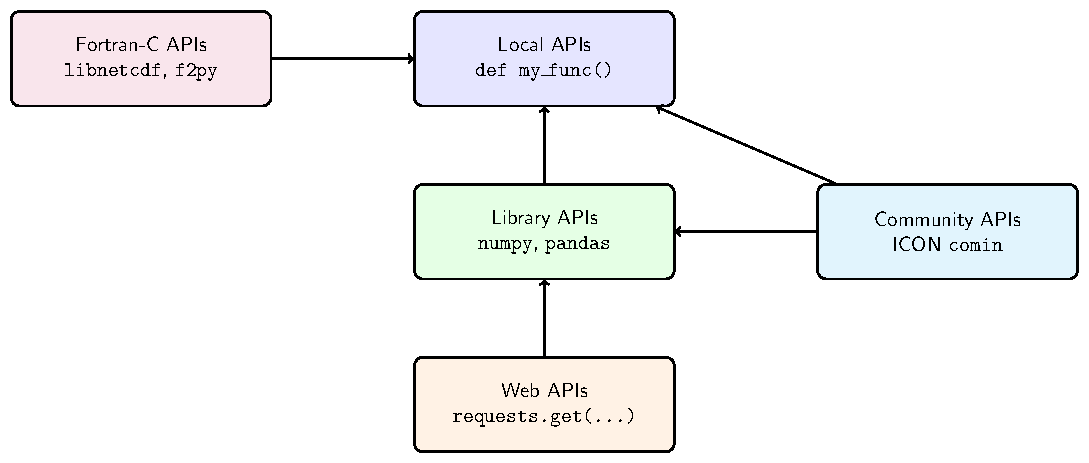
\includegraphics[width=0.8\textwidth]{chapters/api_diagram.pdf}}
	\caption{Importance of API design and functionality.}
\end{figure}
\end{center}%

APIs work by exposing specific methods or endpoints that other code can call. For example, a Python module can expose a function like \texttt{add(a, b)}, or a web service can expose an HTTP endpoint like \texttt{/weather?city=Berlin}. In both cases, the underlying logic is hidden, and only the necessary interface is visible. This separation is crucial for code maintenance and scalability.

%==============================================================================
%
%==============================================================================
\subsection{Why Learn APIs from the Beginning?}

APIs are not just an advanced tool but a \bbb{fundamental principle of code development} that should be learned from the start. Here’s why:
\begin{itemize}
    \item \bbb{Modularity:} APIs encourage splitting code into independent modules, making it easier to test, maintain, and extend.
    \item \bbb{Reusability:} Functions and classes defined in one project can be reused across different projects through APIs.
    \item \bbb{Collaboration:} APIs allow teams to work on different components simultaneously, with clearly defined interfaces.
    \item \bbb{Abstraction:} Details are hidden behind the API, exposing only what is necessary, which helps avoid unnecessary complexity.
    \item \bbb{Scalability:} As projects grow, APIs provide a stable way to integrate new features without breaking existing code.
\end{itemize}

APIs are \bbb{everywhere in Python development}, from the built-in functions of the standard library to external packages like \texttt{numpy} or \texttt{pandas}. When working with data, machine learning models, or even complex weather systems, APIs help organize the code logically and efficiently.

We use APIs in many places for AI/ML development. It is there for data provision. It defines the connection between {\bf user interfaces}, the {\bf server} managing user requests, the {\bf large language model} providing an intelligent service, the {\bf function calls} which link specific functionality into the user-service interaction. 

%==============================================================================
%
%==============================================================================
\subsection{Types of APIs in Python}

APIs in Python can take various forms:
\begin{itemize}
    \item \bbb{Local APIs:} A set of functions or classes within a Python module that can be imported and used in other scripts.
    \item \bbb{Library APIs:} External libraries like \texttt{numpy} or \texttt{pandas} expose APIs that developers use for numerical operations or data manipulation.
    \item \bbb{Web APIs:} Services like \texttt{OpenWeatherMap} or \texttt{PokeAPI} provide data over HTTP, which Python can access using tools like \texttt{requests}.
\end{itemize}

%==============================================================================
%
%==============================================================================
\subsection{APIs as a Structuring Principle for Code Development}

From the beginning of your Python learning journey, understanding and using APIs helps build \bbb{structured, maintainable, and scalable code}. APIs force developers to think about clear interfaces, modular design, and reusability, which are essential practices in any project, large or small.

In this tutorial, we will explore both local and web APIs, demonstrating how to create and consume APIs to build powerful and efficient Python applications.

%==============================================================================
%
%==============================================================================
\section{Making API Requests with \texttt{requests}}

In modern software development, REST APIs have become a standard method for enabling communication between distributed components. The API we developed in \texttt{code011\_REST.py} uses the Flask framework to expose endpoints that allow operations such as creating, reading, updating, and deleting items. This design follows the REST principles by ensuring a stateless, client–server interaction with a clear separation of concerns. On the server side, we define endpoints like \texttt{/items} for retrieving or adding items, and \texttt{/items/<id>} for working with individual items.

The client implementation, found in \texttt{code012\_REST\_client.py}, leverages the Python \texttt{requests} library to interact with these endpoints. This library abstracts the details of HTTP communication and provides simple functions for GET, POST, PUT, and DELETE requests. By using \texttt{requests}, developers can focus on the application logic rather than on low-level network details.

\bigskip

\textbf{Setting Up the Server:}\\
In \texttt{code011\_REST.py}, the Flask server is set up to listen on a local port (usually 5000). The code defines several endpoints:
\begin{itemize}
  \item \textbf{GET /items}: Returns the entire collection of items as JSON.
  \item \textbf{GET /items/<id>}: Retrieves a specific item by its identifier.
  \item \textbf{POST /items}: Accepts JSON data to create a new item. The new item’s identifier is generated automatically and also allows client-specified IDs.
  \item \textbf{PUT /items/<id>}: Updates an existing item.
  \item \textbf{DELETE /items/<id>}: Removes an item from the collection.
  \item \textbf{POST /items/<id>/upload}: Uploads a file associated with an item. The server saves the file in a designated uploads directory and records the file path in the item's data.
  \item \textbf{GET /items/<id>/download}: Downloads the file associated with an item. The server retrieves the stored file and sends it as an attachment, allowing the client to save it with its original filename.
\end{itemize}

\begin{center}
\begin{figure}[ht]
   \centerline{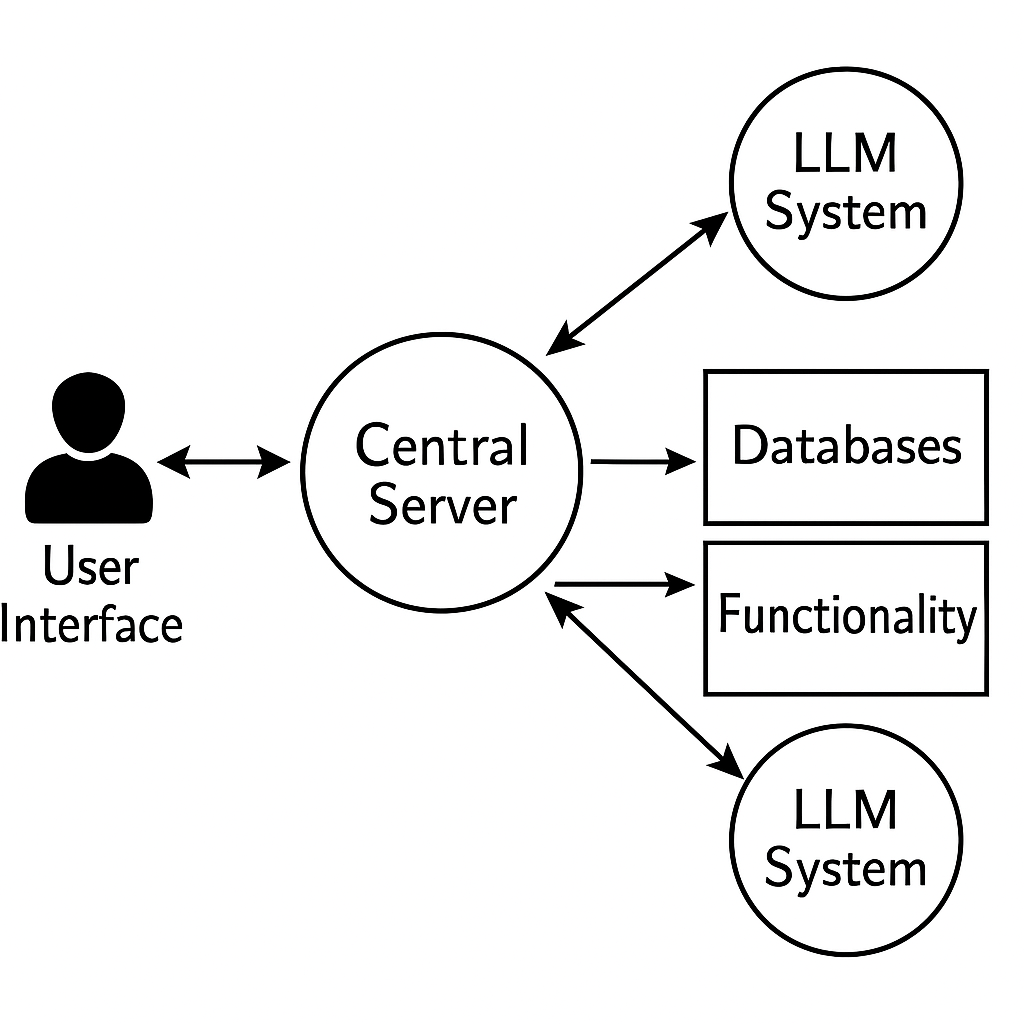
\includegraphics[width=0.5\textwidth]{images/user-server-database-llm.png}}
	\caption{How APIs are crucial for AI/ML applications involving large language models (LLM) with user services. The {\bf user interface} interacts with the {\bf central server} through an API. The server uses APIs to talk to the {\bf LLMs}. It uses APIs for {\bf database requests} (including the user and rights management, but also to pull observations, fields, analyses and much more. It also interacts with specific {\bf functionality} providing \textcolor{DWDblue}{\bf weather and climate services}, including sophisticated AI/ML applications, through further APIs.}
\end{figure}
\end{center}%

We have the full server code as demo application in the file \texttt{flask\_server\_request\_api.py}. Here, we explain its components: 

{\bf Server Setup.} We start by importing necessary modules and creating the Flask app instance.

\begin{codeonly}{Setup}
from flask import Flask, jsonify, request, abort, send_from_directory
from werkzeug.utils import secure_filename
import os

app = Flask(__name__)
\end{codeonly}

{\bf Upload Folder and Allowed Extensions.} Define the upload folder and allowed file types.

\begin{codeonly}{Upload Configuration}
UPLOAD_FOLDER = 'uploads'
ALLOWED_EXTENSIONS = {'txt', 'pdf', 'png', 'jpg', 'jpeg', 'gif'}

if not os.path.exists(UPLOAD_FOLDER):
    os.makedirs(UPLOAD_FOLDER)

def allowed_file(filename):
    return '.' in filename and \
           filename.rsplit('.', 1)[1].lower() in ALLOWED_EXTENSIONS
\end{codeonly}

{\bf In-Memory Item List.} A simple list of items simulates a database.

\begin{codeonly}{Initial Items}
items = [
    {"id": 1, "name": "Item 1"},
    {"id": 2, "name": "Item 2"},
]
\end{codeonly}

{\bf GET /items.} Return all items.

\begin{codeonly}{GET /items}
@app.route('/items', methods=['GET'])
def get_items():
    return jsonify(items)
\end{codeonly}

{\bf GET /items/<id>.} Return a single item by ID.

\begin{codeonly}{GET /items/<id>}
@app.route('/items/<int:item_id>', methods=['GET'])
def get_item(item_id):
    item = next((item for item in items if item['id'] == item_id), None)
    if item is None:
        abort(404)
    return jsonify(item)
\end{codeonly}

{\bf POST /items.} Add a new item.

\begin{codeonly}{POST /items}
@app.route('/items', methods=['POST'])
def create_item():
    if not request.json or 'name' not in request.json:
        abort(400)
    new_item = {
        "id": items[-1]["id"] + 1 if items else 1,
        "name": request.json['name']
    }
    items.append(new_item)
    return jsonify(new_item), 201
\end{codeonly}

{\bf PUT /items/<id>.} Update or create an item by ID.

\begin{codeonly}{PUT /items/<id>}
@app.route('/items/<int:item_id>', methods=['PUT'])
def update_or_create_item(item_id):
    if not request.json or 'name' not in request.json:
        abort(400)
    item = next((item for item in items if item['id'] == item_id), None)
    if item is None:
        new_item = {"id": item_id, "name": request.json['name']}
        items.append(new_item)
        return jsonify(new_item), 201
    else:
        item['name'] = request.json.get('name', item['name'])
        return jsonify(item)
\end{codeonly}

{\bf DELETE /items/<id>.} Delete an item.

\begin{codeonly}{DELETE /items/<id>}
@app.route('/items/<int:item_id>', methods=['DELETE'])
def delete_item(item_id):
    global items
    items = [item for item in items if item['id'] != item_id]
    return jsonify({'result': True})
\end{codeonly}

{\bf POST /items/<id>/upload.} Upload a file for a specific item.

\begin{codeonly}{POST /items/<id>/upload}
@app.route('/items/<int:item_id>/upload', methods=['POST'])
def upload_file(item_id):
    item = next((item for item in items if item['id'] == item_id), None)
    if item is None:
        abort(404)
    if 'file' not in request.files:
        abort(400, description="No file part in the request")
    file = request.files['file']
    if file.filename == '':
        abort(400, description="No selected file")
    if file and allowed_file(file.filename):
        filename = secure_filename(file.filename)
        saved_filename = f"{item_id}_{filename}"
        file_path = os.path.join(UPLOAD_FOLDER, saved_filename)
        file.save(file_path)
        item['file'] = file_path
        return jsonify({'result': 'File uploaded', 'file_path': file_path}), 201
    else:
        abort(400, description="File type not allowed")
\end{codeonly}

{\bf GET /items/<id>/download.} Download a file attached to an item.

\begin{codeonly}{GET /items/<id>/download}
@app.route('/items/<int:item_id>/download', methods=['GET'])
def download_file(item_id):
    item = next((item for item in items if item['id'] == item_id), None)
    if item is None or 'file' not in item:
        abort(404)
    file_path = item['file']
    directory, filename = os.path.split(file_path)
    return send_from_directory(directory, filename, as_attachment=True)
\end{codeonly}

{\bf Start the Server.} Run the application in debug mode.

\begin{codeonly}{Run Server}
if __name__ == '__main__':
    app.run(debug=True)
\end{codeonly}

This server code, which you can view in detail in \texttt{flask\_server\_request\_api.py}, serves as the API’s backend. The careful design ensures that the API is both stateless and uniform, allowing clients to interact predictably with the service.

\bigskip
\textbf{Interacting with the API Using \texttt{requests}:}\\
On the client side, \texttt{code012\_REST\_client.py} demonstrates how to use the \texttt{requests} library to make calls to our API. Let’s consider a few typical examples:

\begin{enumerate}
  \item \textbf{Retrieving All Items:}\\  
  A simple GET request is used to fetch the list of items. The client code sends:
  \begin{verbatim}
response = requests.get('http://127.0.0.1:5000/items')
print(response.json())
  \end{verbatim}
  This call returns a JSON array containing all items. By decoding the response, the client can easily process and display the data.

  \item \textbf{Retrieving a Specific Item:}\\  
  To fetch an individual item, the client sends a GET request with the item’s ID in the URL:
  \begin{verbatim}
response = requests.get('http://127.0.0.1:5000/items/1')
print(response.json())
  \end{verbatim}
  If the item exists, the server returns its details in JSON format; if not, an error (typically a 404 Not Found) is returned.

  \item \textbf{Adding a New Item:}\\  
  The POST request is used to create a new item. In our implementation, the client sends a JSON payload:
  \begin{verbatim}
new_item = {'name': 'New Item'}
response = requests.post('http://127.0.0.1:5000/items', json=new_item)
print(response.json())
  \end{verbatim}
  The server then generates a new item with a unique ID and returns it. Notice that the \texttt{json=} parameter in the request call makes it easy to send JSON data without manual serialization.

  \item \textbf{Updating and Deleting Items:}\\  
  Similarly, PUT requests are used to update an item and DELETE requests to remove it. The corresponding code in \texttt{code012\_REST\_client.py} handles these actions by specifying the correct URL endpoints and sending appropriate JSON data if necessary.
	
	\item \textbf{Upload Functionality:}\\  
In addition to updating and deleting items, the REST API example demonstrates file uploads. Clients can attach files to specific items by sending a POST request to an endpoint such as \texttt{/items/\textless id\textgreater/upload}. This endpoint accepts multipart form-data where the file is provided under a designated field (e.g., \texttt{'file'}). On the server side, Flask processes the incoming file, ensures its name is secured using \texttt{secure\_filename}, and then saves it into a dedicated uploads directory. The file path is subsequently stored in the item's record, associating the file with the item. This approach enables users to easily manage additional resources related to each item.

\item \textbf{Download Functionality:}\\  
Complementing the upload feature, the API also provides a download endpoint at \linebreak\texttt{/items/\textless id\textgreater/download}. When a client sends a GET request to this endpoint, the server locates the file associated with the item and transmits it back as an attachment using Flask's \texttt{send\_from\_directory} function. This not only ensures that the file is delivered with the correct MIME type but also prompts the client’s browser to download it rather than display it inline. On the client side, the downloaded file can be saved with its original name by removing any item-specific prefixes that were added during upload, thus preserving the original filename. This integrated upload and download mechanism enhances the functionality of the REST API by allowing it to handle both data and associated file resources seamlessly.

\end{enumerate}

\begin{codeonly}{}
import requests

# Base URL of the API
base_url = 'http://127.0.0.1:5000'

# GET all items
response = requests.get(f'{base_url}/items')
print("GET /items:", response.json())

# GET a specific item (e.g., id = 1)
response = requests.get(f'{base_url}/items/1')
print("GET /items/1:", response.json())

# POST a new item
new_item = {'name': 'New Item'}
response = requests.post(f'{base_url}/items', json=new_item)
print("POST /items:", response.json())

# PUT to update an item (e.g., id = 1)
updated_item = {'name': 'Updated Item 1'}
response = requests.put(f'{base_url}/items/1', json=updated_item)
print("PUT /items/1:", response.json())

# DELETE an item (e.g., id = 1)
response = requests.delete(f'{base_url}/items/1')
print("DELETE /items/1:", response.json())

# Check items after deletion
response = requests.get(f'{base_url}/items')
print("GET /items after deletion:", response.json())

# -------------------------
# UPLOAD a file for an item (e.g., for item with id = 2)
upload_url = f'{base_url}/items/2/upload'
# Ensure you have a file named 'example.txt' in your current directory
with open('example.txt', 'rb') as f:
    files = {'file': f}
    response = requests.post(upload_url, files=files)
    print("POST /items/2/upload:", response.json())

# -------------------------
# DOWNLOAD the file associated with an item (e.g., for item with id = 2)
download_url = f'{base_url}/items/2/download'
response = requests.get(download_url, stream=True)
if response.status_code == 200:
    # Save the downloaded file locally
    with open('downloaded_example.txt', 'wb') as f:
        for chunk in response.iter_content(chunk_size=8192):
            f.write(chunk)
    print("File downloaded successfully and saved as downloaded_example.txt")
else:
    print("Failed to download file, status code:", response.status_code)
\end{codeonly}


\textbf{Error Handling and Debugging:}\\
A crucial aspect of making API requests is managing errors gracefully. The client code checks the HTTP status code returned by the server and handles error responses appropriately. For instance, if a GET request for an item returns a 404 status code, the client can notify the user that the requested item does not exist. Similarly, for POST and PUT requests, verifying that the server returns the expected 201 or 200 status code helps ensure that operations have completed successfully.

\bigskip

\textbf{Benefits of This Approach:}\\
Using the \texttt{requests} library to interact with our REST API provides several benefits:
\begin{itemize}
  \item \textbf{Simplicity:} The \texttt{requests} library offers an intuitive API that abstracts the complexity of HTTP communication.
  \item \textbf{Flexibility:} Developers can easily extend the client to support additional endpoints or incorporate authentication mechanisms.
  \item \textbf{Maintainability:} By separating the server (\texttt{code011\_REST.py}) and client (\texttt{code012\_REST\_client.py}) code, our architecture is modular. This makes it easier to update one component without affecting the other.
  \item \textbf{Reusability:} The external code inclusion method using \texttt{\textbackslash includeexternalcode} promotes code reuse and ensures that our documentation is consistent with our source code.
\end{itemize}

It is now very easy to define simple functions such as \texttt{list()}, \texttt{up(<filename>,<id>)} or \texttt{down(<id>)} to list all uploaded items, to upload a particular file or to download a particular file. 

\bigskip
In summary, making API requests with Python’s \texttt{requests} library is both straightforward and powerful. Our implementation demonstrates a complete cycle: setting up a REST API server with Flask, handling standard HTTP methods, and interacting with the API via a client script. The combination of clear server endpoints, robust client-side error handling, and modular code inclusion makes this approach a solid foundation for building scalable and maintainable web services.

\bigskip

By following these practices, you can build reliable applications that communicate over HTTP in a standardized way, ultimately leading to more effective and efficient software systems.

\begin{recommendationbox}
An API-centric mindset greatly enhances fast development, modular design, and clean separation of responsibilities.
\end{recommendationbox}

%================================================================================
%
%================================================================================
\section{Fortran Integration using \texttt{ctypes} as API}

In this section, we illustrate an approach to integrating FORTRAN code with Python by using the \texttt{ctypes} module. The library \texttt{ctypes} provides explicit control over data types and memory management when interfacing with compiled shared libraries.

\begin{center}
\begin{figure}[ht]
   \centerline{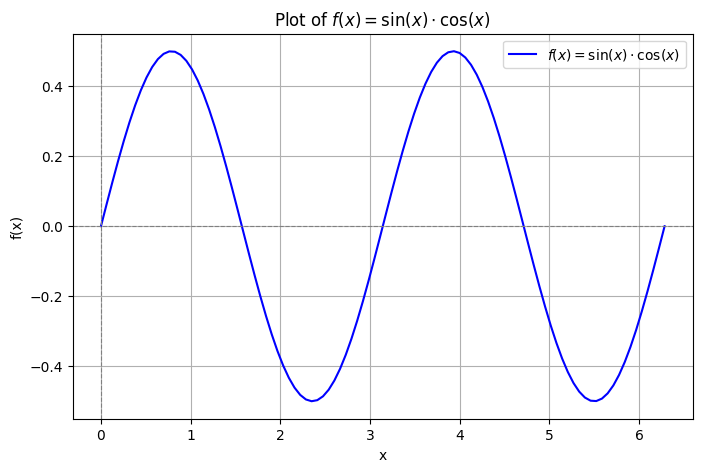
\includegraphics[width=0.6\textwidth]{images/sin_cos.png}}
	\caption{We use the Fortran \texttt{iso\_c\_binding module} to create a C-compatible API, allowing Fortran routines to be called from C or other languages such as Python via ctypes or f2py.}
\end{figure}
\end{center}%

The following example demonstrates how to load a Fortran shared library (compiled as \linebreak\texttt{fortran\_interface.so}), define the function prototype for the Fortran function \texttt{f\_sin\_cos}, and compute the function \( f(x) = \sin(x) \cdot \cos(x) \) for 100 values between 0 and \(2\pi\). The computed values are then plotted using Matplotlib. Additionally, the code checks for the existence of a Fortran debug log and prints its contents if available.

%\includeexternalcode{Fortran Module: code013\_fortran\_interface.f90}{code013_fortran_interface.f90}
\begin{codeonly}{FORTRAN code example}
%%writefile fortran_interface.f90
module fortran_module
    use iso_c_binding, only: c_double
    implicit none
contains
    function f_sin_cos(x) result(f) bind(C, name="f_sin_cos")
        implicit none
        real(c_double), intent(in) :: x
        real(c_double) :: f
        f = sin(x) * cos(x)
    end function f_sin_cos
end module fortran_module
\end{codeonly}

Compile this based on gfortran. 

\begin{codeonly}{Compilation}
gfortran -shared -fPIC fortran_interface.f90 -o fortran_interface.so
\end{codeonly}

Then, you might use the code, e.g.\ in a jupyter notebook or as basic python application. 

It can be extremely helpful to make your fortran modules and functions available for execution in your python framework. We will pursue this further in upcoming parts of this tutorial.

%================================================================================
%
%================================================================================


 % Jupyter Notebooks, Clouds and Servers
\chapter{Eccodes for Grib, Opendata, NetCDF, Visualization}

Meteorological data are often stored in GRIB or NetCDF formats, both of which are compact binary formats widely used in numerical weather prediction and climate analysis. While GRIB is the standard format for meteorological model outputs, NetCDF is more commonly used in the broader scientific community, particularly for observational datasets and climate research. Additionally, Zarr is an alternative format to NetCDF, optimized for cloud-based storage and parallel computing for machine learning applications. Recent developments allow storing NetCDF data in Zarr format for enhanced scalability.

In this chapter, we demonstrate how to work with both formats, focusing on GRIB data using the ECCODES library---provided by ECMWF---to decode and analyze meteorological data from the {\em DWD Open Data Server}, and working with NetCDF for further integration and analysis. We will cover the following steps:

\begin{itemize}
    \item {\em Accessing and Downloading GRIB Data}: Retrieving ICON model GRIB files, including latitude-longitude fields and the 2-m temperature field, from the DWD Open Data Server.
    \item {\em Inspecting GRIB File Metadata}: Listing GRIB file keys, understanding metadata, and summarizing the available parameters and levels.
    \item {\em Loading and Visualizing GRIB Data}: Extracting numerical fields, mapping the spatial coordinates, and plotting meteorological variables using visualization tools.
\end{itemize}

In addition, we introduce NetCDF as a fundamental format for meteorological and climate data, covering the following aspects:

\begin{itemize}
    \item {\em Accessing and Managing NetCDF Data}: Understanding the structure of NetCDF files, reading data, and managing metadata.
    \item {\em Working with NetCDF Data}: Processing and analyzing NetCDF datasets in the context of meteorological applications.
    \item {\em Visualizing NetCDF Data}: Plotting and interpreting NetCDF data using scientific computing tools.
\end{itemize}

By following these steps, we will gain a complete workflow for handling ICON model GRIB and NetCDF files, from downloading and inspection to visualization and analysis for scientific applications.


%==============================================================================
%
%==============================================================================
\section{Downloading ICON Model GRIB Files from DWD Open Data Server}

To analyze meteorological data using the ICON model, we need to download the required GRIB files from the \emph{DWD Open Data Server}. These include the \emph{2-meter temperature field} (\texttt{icon\_t2m.grib}), the \emph{latitude grid} (\texttt{icon\_lat.grib}), and the \emph{longitude grid} (\texttt{icon\_lon.grib}). DWD provides these files in compressed GRIB2 format (\texttt{.grib2.bz2}), which must be downloaded and extracted before further processing. 

{\bf Downloading the 2-Meter Temperature Field.} 

The following script constructs the filename for the \emph{latest 2m temperature GRIB file} based on the current UTC date, downloads it using \texttt{wget}, and extracts it.

\begin{codeonly}{Downloading 2m Temperature Data}
import datetime
import os
import wget
import bz2

# Construct the filename based on the current UTC date
now = datetime.datetime.now(datetime.UTC)
filename = f"icon_global_icosahedral_single-level_{now:%Y%m%d}00_000_T_2M.grib2.bz2"
print("Constructed filename:", filename)

# Define the base URL
base_url = "https://opendata.dwd.de/weather/nwp/icon/grib/00/t_2m/"
url = base_url + filename
print("Download URL:", url)

# Download the .bz2 file using Python wget
wget.download(url, filename)
print(f"\nDownloaded {filename}")

# Decompress the .bz2 file using bz2 module
with bz2.open(filename, 'rb') as f_in, open(filename[:-4], 'wb') as f_out:
    f_out.write(f_in.read())
print(f"Decompressed {filename} to {filename[:-4]}")

# Rename to a standard name
grib_filename = filename[:-4]
final_filename = "icon_t2m.grib"
os.rename(grib_filename, final_filename)
print(f"Renamed {grib_filename} to {final_filename}")
\end{codeonly}

This script ensures that the latest available \emph{2m temperature} field will be automatically retrieved and prepared for use.

{\bf Downloading Latitude and Longitude Data.} 

The latitude (\texttt{icon\_lat.grib}) and longitude (\texttt{icon\_lon.grib}) grids are \emph{time-invariant} and must be downloaded separately. The script below identifies the latest available version on the DWD server, downloads both files, and renames them for easier access. The following script is contained in the file \texttt{icon\_grid\_get.py} as well as in the jupyter notebook to catch forecasts from the DWD open data server. 

\begin{codeonly}{Downloading ICON Latitude and Longitude GRIB Data}
import re
import os
import bz2
import requests
import wget

base_url = "https://opendata.dwd.de/weather/nwp/icon/grib/00/"
clat_path = "clat/"
clon_path = "clon/"

# Function to find the latest available timestamp from DWD server
def get_latest_timestamp(path):
    listing_url = base_url + path
    response = requests.get(listing_url)
    if response.status_code != 200:
        raise RuntimeError(f"Could not fetch listing: {listing_url}")
    timestamps = re.findall(
        r'icon_global_icosahedral_time-invariant_(\d{10})_CLAT\.grib2\.bz2',
        response.text
    )
    return max(timestamps) if timestamps else None

# Get the latest available timestamp
timestamp = get_latest_timestamp(clat_path)
if not timestamp:
    raise RuntimeError("Could not determine latest timestamp from DWD server.")

files = {
    "clat": f"clat/icon_global_icosahedral_time-invariant_{timestamp}_CLAT.grib2.bz2",
    "clon": f"clon/icon_global_icosahedral_time-invariant_{timestamp}_CLON.grib2.bz2"
}

rename_map = {"clat": "icon_lat.grib", "clon": "icon_lon.grib"}

for key, path in files.items():
    filename = os.path.basename(path)
    url = base_url + path

    print(f"Downloading {url} ...")
    wget.download(url, filename)
    print(f"\nDownloaded {filename}")

    # Uncompress the .bz2 file
    with bz2.open(filename, 'rb') as compressed, open(filename[:-4], 'wb') as out_file:
        out_file.write(compressed.read())
    print(f"Decompressed {filename} to {filename[:-4]}")

    # Rename the extracted file
    extracted_filename = filename[:-4]  # Remove .bz2
    new_filename = rename_map[key]
    os.rename(extracted_filename, new_filename)
    print(f"Renamed {extracted_filename} to {new_filename}")
\end{codeonly}

This script identifies the \emph{latest available latitude and longitude files} on the DWD server, downloads them using \texttt{wget}, extracts the \texttt{.bz2} compressed files, and renames them to \texttt{icon\_lat.grib} and \texttt{icon\_lon.grib} for easy reference.

After executing these scripts, we have all necessary \emph{spatial coordinate data and temperature fields} to proceed with further analysis and visualization.


%==============================================================================
%
%==============================================================================
\section{The Grib Library eccodes}

We have discussed the download of grib data, here we now assume that we have icon lat and lon coordinates in files \texttt{icon\_lat.grib} and  \texttt{icon\_lon.grib}. 

\texttt{ecCodes} is a library developed by ECMWF for decoding and encoding GRIB (GRIdded Binary) files. It provides a Python interface to inspect and manipulate meteorological data stored in the GRIB format.

{\bf Installing ecCodes.} Installing \texttt{ecCodes}, the ECMWF library for GRIB file handling, can be challenging due to dependencies and system configurations. Here is a summary of the installation process:

{\bf System Dependencies}: Ensure required system libraries are installed:
\begin{lstlisting}
sudo apt update && sudo apt install libeccodes-dev eccodes
\end{lstlisting}
On macOS, use Homebrew:
\begin{lstlisting}
brew install eccodes
\end{lstlisting}

{\bf Python Package}: Install the Python bindings with:
\begin{verbatim}
pip install eccodes
\end{verbatim}

\begin{recommendationbox}
Using ECCODES on Windows should be done via windows subsystem for linux or through a docker container. 
\end{recommendationbox}

On Windows, you should use the {\bf WSL} (Windows Subsystem for Linux). Here, you can do the same install commands
\begin{lstlisting}
sudo apt update
sudo apt install eccodes
sudo apt install libeccodes-tools
\end{lstlisting}

Test it with 
\begin{lstlisting}
grib_ls -V
\end{lstlisting}

{\bf Setting Environment Variables}: If the library is not found, define the paths manually:
\begin{lstlisting}
export ECCODES_DEFINITION_PATH=/usr/share/eccodes/definitions
export ECCODES_SAMPLES_PATH=/usr/share/eccodes/samples
\end{lstlisting}
Adjust these paths according to your system setup.

{\bf Verifying Installation}: Check if ecCodes is working correctly:
\begin{lstlisting}
grib_ls --help
python -c "import eccodes; print(eccodes.codes_get_api_version())"\end{lstlisting}
If these commands return valid output, the installation is successful.

{\bf Handling DWD-Specific Definitions}: If working with DWD GRIB files, additional definition files may be required. Download the latest version from:
\begin{lstlisting}
https://opendata.dwd.de/weather/lib/grib/
\end{lstlisting}
We provide a script \texttt{download\_latest\_grib\_definition\_dwd.py} which will carry out the download and installation, but still needs you to take care of the path variables. 
Please check and make sure the definitions paths are set properly. 


{\bf Checking if ecCodes is Installed}
Before using \texttt{ecCodes}, you can check if it is installed correctly with the following code:

\begin{codeonly}{Checking ecCodes Installation}
try:
    import eccodes
    print("ecCodes is installed and working correctly.")
except ImportError:
    print("ecCodes is not installed. Please install it using 'pip install eccodes'.")
    exit(1)
\end{codeonly}


{\bf Inspecting Grib Files.}
We next demonstrate how to inspect the metadata keys and shortnames of GRIB files (\texttt{icon\_lat.grib} and \texttt{icon\_lon.grib}) using \texttt{ecCodes}.

{\bf Listing GRIB Keys.} The function below extracts and lists metadata keys from a GRIB file:

\begin{codeonly}{Listing GRIB Keys}
import eccodes

def list_grib_keys(grib_filename):
    """Lists keys from a GRIB file while handling errors properly."""
    try:
        with open(grib_filename, 'rb') as f:
            while True:
                gid = eccodes.codes_grib_new_from_file(f)
                if gid is None:  # End of file
                    break

                key_iterator = eccodes.codes_keys_iterator_new(gid)
                keys = []

                while eccodes.codes_keys_iterator_next(key_iterator):
                    keyname = eccodes.codes_keys_iterator_get_name(key_iterator)
                    if keyname not in ['section2Padding', 'codedValues', 'values']:
                        try:
                            value = eccodes.codes_get_string(gid, keyname)
                        except Exception:
                            value = "N/A"
                        keys.append((keyname, value))

                eccodes.codes_release(gid)
                
                # Print all extracted keys
                for key, value in keys:
                    print(f"Key: {key:40} Value: {value}")
    except eccodes.CodesInternalError as e:
        print(f"ecCodes Error: {e}")

# Example usage
list_grib_keys("icon_lat.grib")
\end{codeonly}

Output can be e.g.\
\begin{codeonly}{Keys}
Key: globalDomain                             Value: g
Key: GRIBEditionNumber                        Value: 2
Key: tablesVersionLatestOfficial              Value: 32
Key: tablesVersionLatest                      Value: 32
Key: grib2divider                             Value: 1e+06
Key: angleSubdivisions                        Value: 1e+06
Key: missingValue                             Value: 9999
Key: ieeeFloats                               Value: 1
Key: isHindcast                               Value: 0
...
\end{codeonly}


{\bf Listing Short Names from a GRIB File.}

The function below extracts and lists short names along with their corresponding levels and sizes from a GRIB file:

\begin{codeonly}{Listing Short Names}
import eccodes

def show_shortnames(grib_file):
    """Lists short names, levels, and sizes from a GRIB file."""
    with open(grib_file, 'rb') as f:
        shortName_prev = ''
        output = ''
        level_prev = ''
        count = 0
        print('-' * 80)
        print('File = ', grib_file)
        print('\n{:<30}{:<16}{:>10}'.format('Short Name', 'Level', 'Size'))
        print('-' * 80)
        while True:
            gid = eccodes.codes_grib_new_from_file(f)
            if gid is None:
                break
            shortName = eccodes.codes_get(gid, "shortName")
            level = eccodes.codes_get(gid, "level")
            size1 = eccodes.codes_get_size(gid, "values")
            if shortName_prev != shortName:
                if level_prev != level and count > 0:
                    output += f' - {level_prev}'
                if count > 0:
                    output += f', \t Size = {size1}'
                output += '\n{:<30}{:<16}{:>10}'.format(shortName, level, size1)
                shortName_prev = shortName
                level_prev = level
                count += 1
            eccodes.codes_release(gid)
        print(output)

# Example usage
show_shortnames("icon_lat.grib")
\end{codeonly}

Output is something like e.g.\

\begin{codeonly}{Shortnames, Levels, Size}
--------------------------------------------------------------------------------
File =  icon_lat.grib
Short Name                    Level                 Size
--------------------------------------------------------------------------------
tlat                          0                  2949120
\end{codeonly}

These functions allow users to inspect the GRIB file structure, understand available variables, and extract key metadata for further analysis.

{\bf Plotting Latitude and Longitude Data.} To visualize the points stored in the GRIB files, we use \texttt{matplotlib} along with \texttt{cartopy} to overlay the scatter plot on a map:

\begin{codeonly}{Plotting Latitude and Longitude with a Map}
import eccodes
import numpy as np
import matplotlib.pyplot as plt
import cartopy.crs as ccrs
import cartopy.feature as cfeature

def plot_lat_lon(lat_file, lon_file):
    """Plots latitude and longitude points from GRIB files on a map."""
    def extract_values(grib_file):
        with open(grib_file, 'rb') as f:
            gid = eccodes.codes_grib_new_from_file(f)
            values = eccodes.codes_get_array(gid, "values")
            eccodes.codes_release(gid)
        return values
    
    latitudes = extract_values(lat_file)
    longitudes = extract_values(lon_file)
    
    plt.figure(figsize=(10, 5))
    ax = plt.axes(projection=ccrs.PlateCarree())
    ax.set_global()
    ax.add_feature(cfeature.LAND, edgecolor='black')
    ax.add_feature(cfeature.COASTLINE)
    ax.add_feature(cfeature.BORDERS, linestyle=':')
    
    plt.scatter(longitudes, latitudes, s=0.5, color='gray', transform=ccrs.PlateCarree())
    plt.xlabel("Longitude")
    plt.ylabel("Latitude")
    plt.title("Scatter Plot of Latitude and Longitude on a Map")
    plt.grid()
    plt.savefig("icon_points_global.png", dpi=300, bbox_inches='tight')
    plt.show()

# Example usage
plot_lat_lon("icon_lat.grib", "icon_lon.grib")
\end{codeonly}

This function:
\begin{itemize}
    \item Reads latitude and longitude values from GRIB files.
    \item Uses \texttt{matplotlib} and \texttt{cartopy} to overlay the points on a global map.
    \item Adds land, coastlines, and country borders for better visualization.
\end{itemize}

\begin{figure}[ht]
    \centering
    \begin{minipage}{0.5\textwidth}
        \centering
        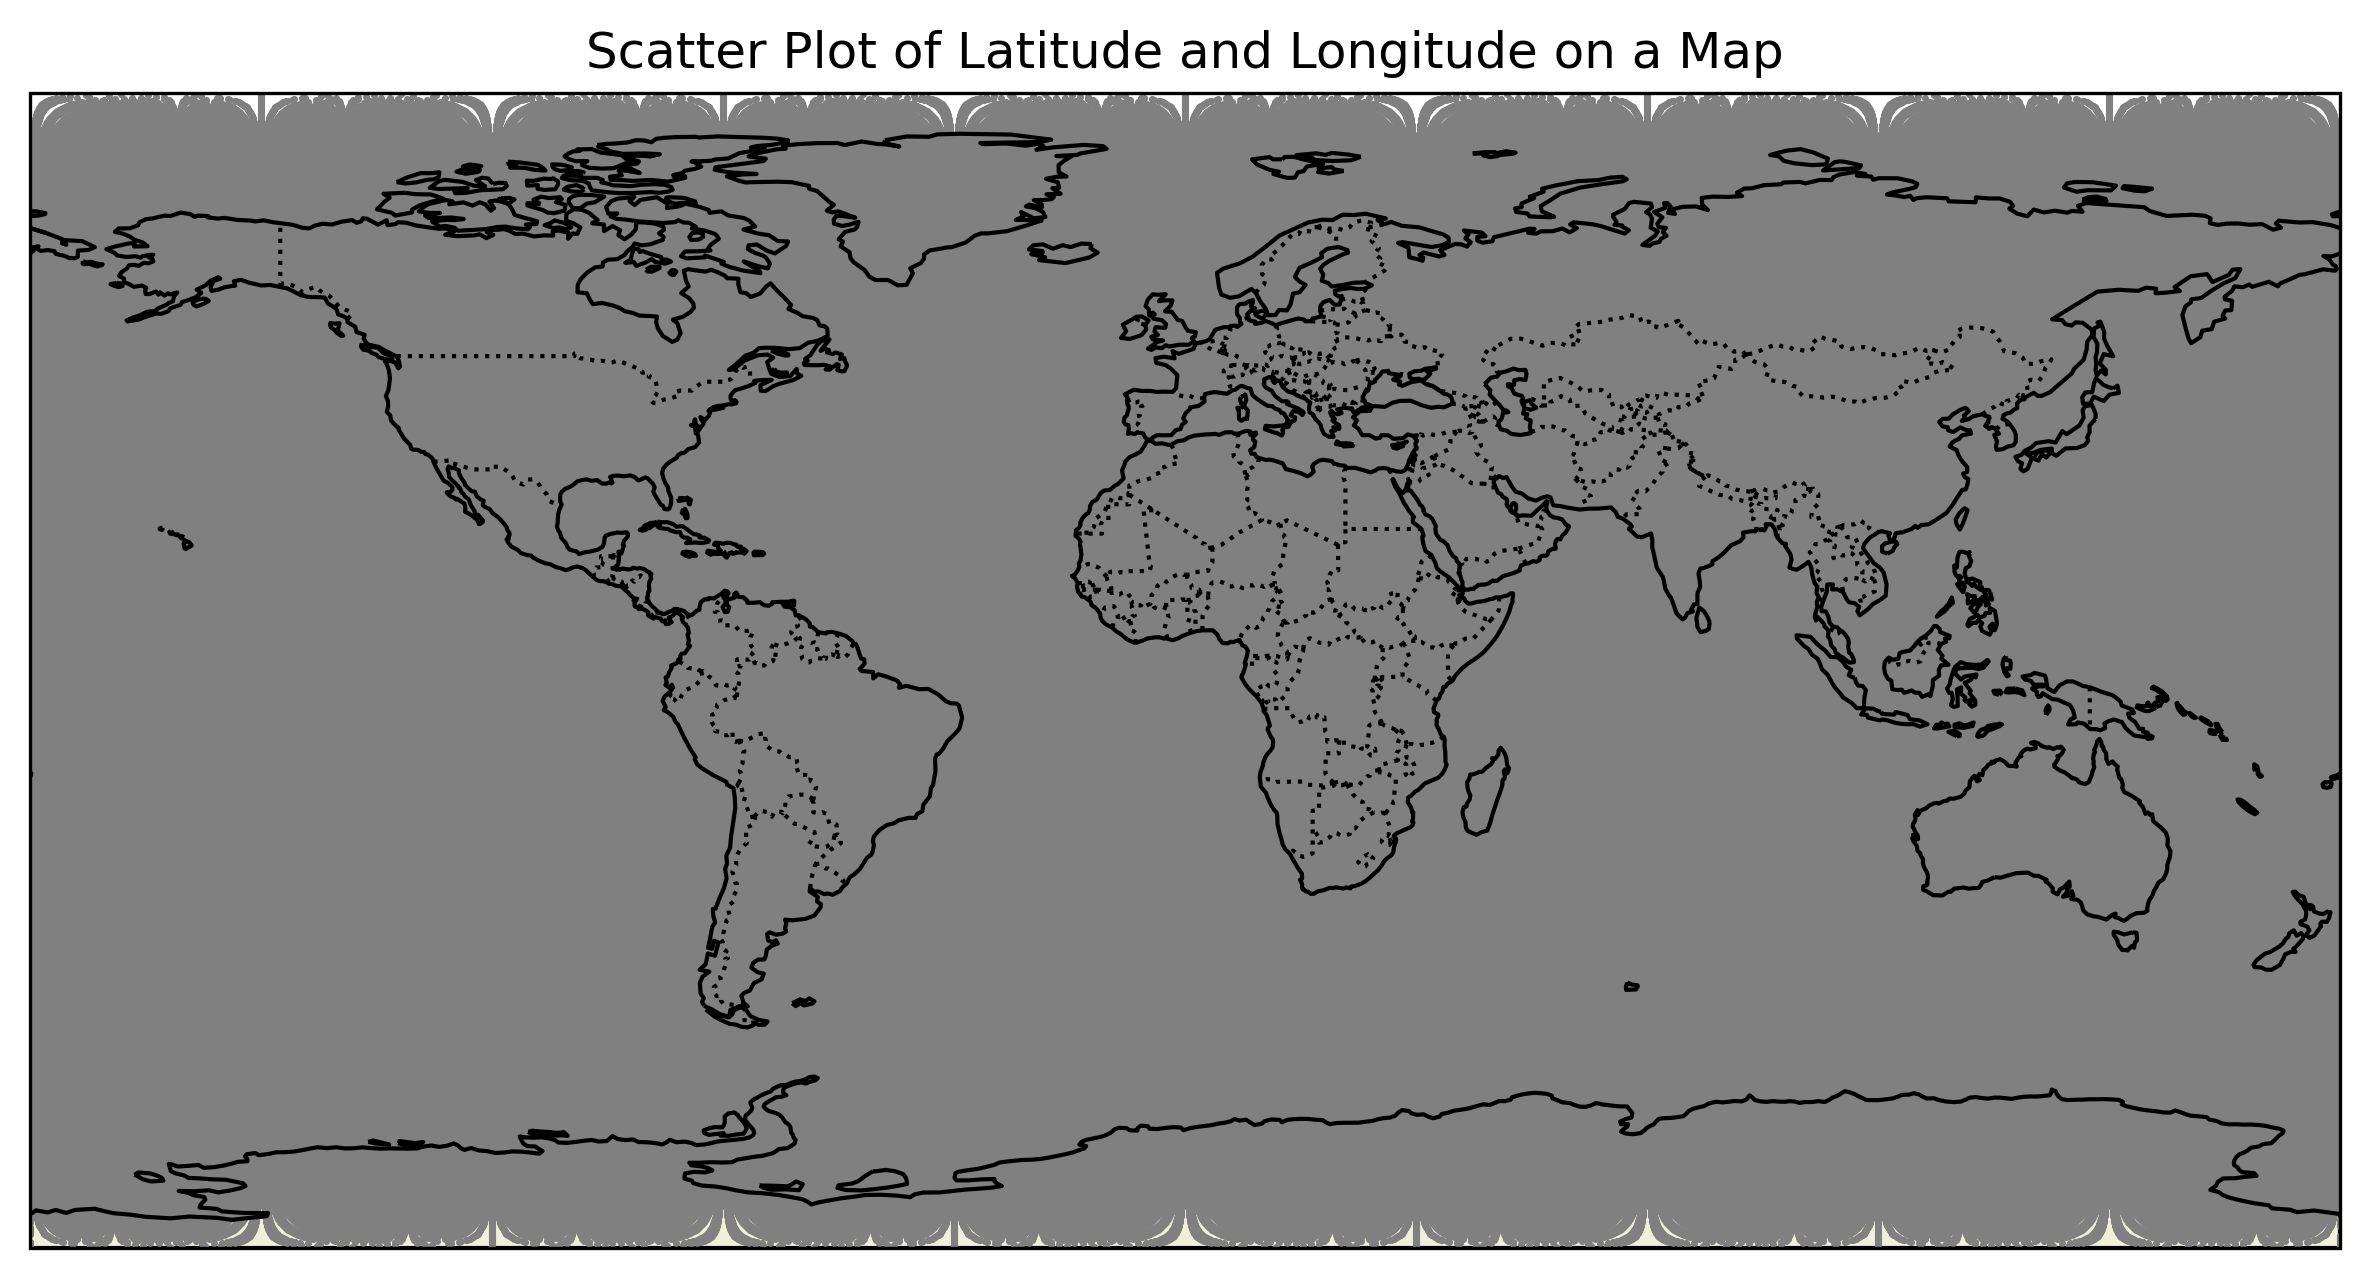
\includegraphics[width=\textwidth]{images/icon_points_global.png}
        \caption{Global ICON grid points.}
        \label{fig:t2m_global_interp}
    \end{minipage}
    \hfill
    \begin{minipage}{0.4\textwidth}
        \centering
        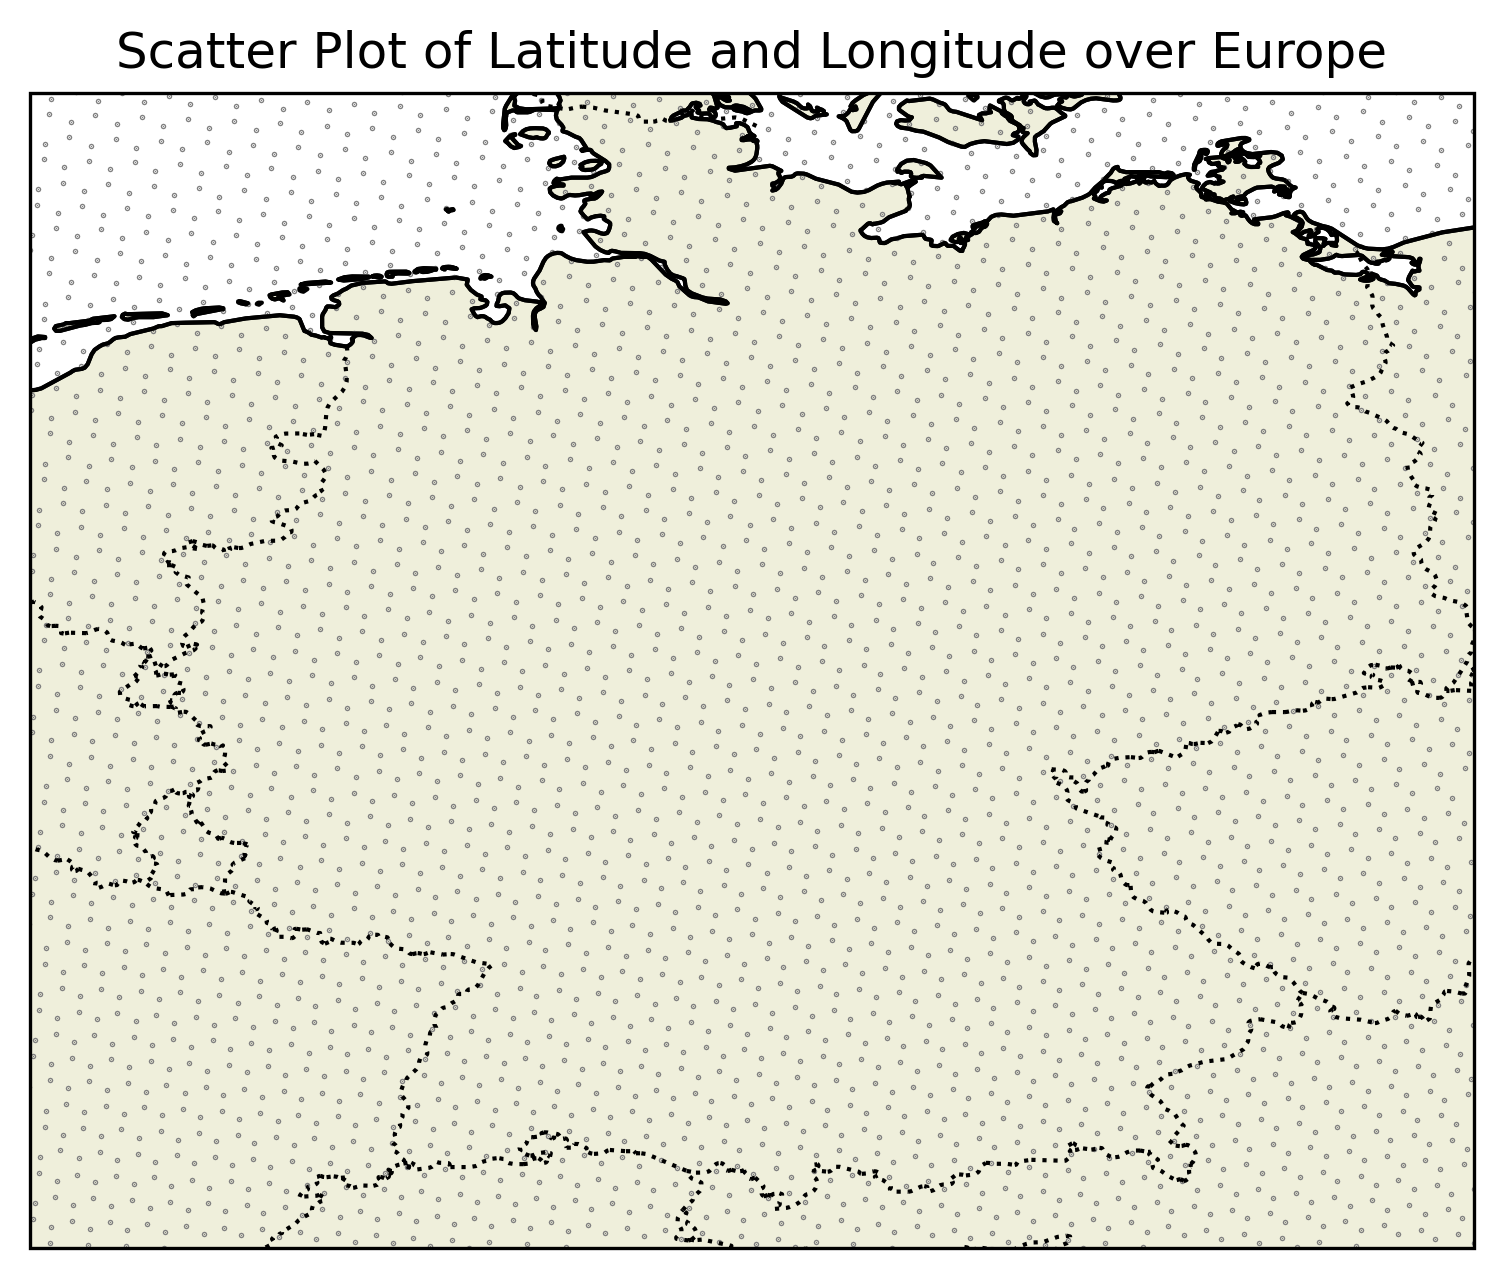
\includegraphics[width=\textwidth]{images/icon_points_germany.png}
        \caption{ICON grid points over Germany.}
        \label{fig:t2m_germany_interp}
    \end{minipage}
\end{figure}

But the resolution is quite high, you cannot see much any more, everything is covered by points. 


{\bf Zooming in Over Germany.} To visualize the points stored in the GRIB files, we use \texttt{matplotlib} along with \texttt{cartopy} to overlay the scatter plot on a map:

\begin{codeonly}{Plotting Latitude and Longitude with a Map}
import eccodes
import numpy as np
import matplotlib.pyplot as plt
import cartopy.crs as ccrs
import cartopy.feature as cfeature

def plot_lat_lon_germany(lat_file, lon_file):
    """Plots latitude and longitude points from GRIB files, zoomed in over Europe."""
    def extract_values(grib_file):
        with open(grib_file, 'rb') as f:
            gid = eccodes.codes_grib_new_from_file(f)
            values = eccodes.codes_get_array(gid, "values")
            eccodes.codes_release(gid)
        return values
    
    latitudes = extract_values(lat_file)
    longitudes = extract_values(lon_file)
    
    plt.figure(figsize=(10, 5))
    ax = plt.axes(projection=ccrs.PlateCarree())
    ax.set_extent([5, 15, 47, 55], crs=ccrs.PlateCarree())  # Europe zoom: [lon_min, lon_max, lat_min, lat_max]
    ax.add_feature(cfeature.LAND, edgecolor='black')
    ax.add_feature(cfeature.COASTLINE)
    ax.add_feature(cfeature.BORDERS, linestyle=':')
    
    plt.scatter(longitudes, latitudes, s=0.1, color='blue', transform=ccrs.PlateCarree())
    plt.xlabel("Longitude")
    plt.ylabel("Latitude")
    plt.title("Scatter Plot of Latitude and Longitude over Europe")
    plt.grid()
    plt.savefig("icon_points_germany.png", dpi=300, bbox_inches='tight')
    plt.show()

# Example usage
plot_lat_lon_germany("icon_lat.grib", "icon_lon.grib")
\end{codeonly}

This function:
\begin{itemize}
    \item Reads latitude and longitude values from GRIB files.
    \item Zooms into Europe with specific latitude/longitude boundaries.
    \item Uses \texttt{matplotlib} and \texttt{cartopy} to overlay the points on a regional map.
    \item Adjusts the point size to avoid excessive density.
\end{itemize}

{\bf Visualizing 2-Meter Temperature (T2M)}

To visualize the 2-meter temperature field from GRIB data, we extract the temperature values alongside the previously loaded latitude and longitude coordinates. The relevant Python function for loading the T2M values is:

\begin{codeonly}{Loading T2M Data}
import eccodes

def load_grib(file, var):
    """Loads specified variable from GRIB file."""
    with open(file, 'rb') as f:
        while (gid := eccodes.codes_grib_new_from_file(f)) is not None:
            if eccodes.codes_get(gid, "shortName") == var:
                vals = eccodes.codes_get_array(gid, "values")
                eccodes.codes_release(gid)
                return vals
            eccodes.codes_release(gid)
    return None

# Load T2M data
t2m = load_grib("icon_t2m.grib", "2t")
\end{codeonly}

Once the temperature values are obtained, they are visualized using \texttt{matplotlib} and \texttt{cartopy}, adapting the point size dynamically based on the bounding box size to maintain clarity across different zoom levels. The visualization function is given below:

\begin{codeonly}{Plotting T2M Data}
import numpy as np
import matplotlib.pyplot as plt
import cartopy.crs as ccrs
import cartopy.feature as cfeature

def plot_t2m(lat, lon, t2m, bbox, title, fname):
    """Plots 2m temperature within bbox = (latmin, latmax, lonmin, lonmax)."""
    latmin, latmax, lonmin, lonmax = bbox
    mask = (lat >= latmin) & (lat <= latmax) & (lon >= lonmin) & (lon <= lonmax)
    
    # Adaptive point size based on bounding box area
    area = (latmax - latmin) * (lonmax - lonmin)
    point_size = max(0.05, min(10, 500 / area))  # Ensures reasonable point size
    
    plt.figure(figsize=(10, 6))
    ax = plt.axes(projection=ccrs.PlateCarree())
    ax.set_extent([lonmin, lonmax, latmin, latmax])
    ax.add_feature(cfeature.LAND, edgecolor='black')
    ax.add_feature(cfeature.COASTLINE)
    ax.add_feature(cfeature.BORDERS, linestyle=':')

    plt.scatter(lon[mask], lat[mask], c=t2m[mask], cmap='jet', s=point_size, transform=ccrs.PlateCarree())
    plt.colorbar(label="Temp (K)")
    plt.title(title)
    plt.savefig(fname, dpi=300, bbox_inches='tight')
    plt.show()
\end{codeonly}

Using this function, we generate two figures displaying the global distribution of 2-meter temperature and a zoomed-in view over Germany.

\begin{figure}[ht]
    \centering
    \begin{minipage}{0.5\textwidth}
        \centering
        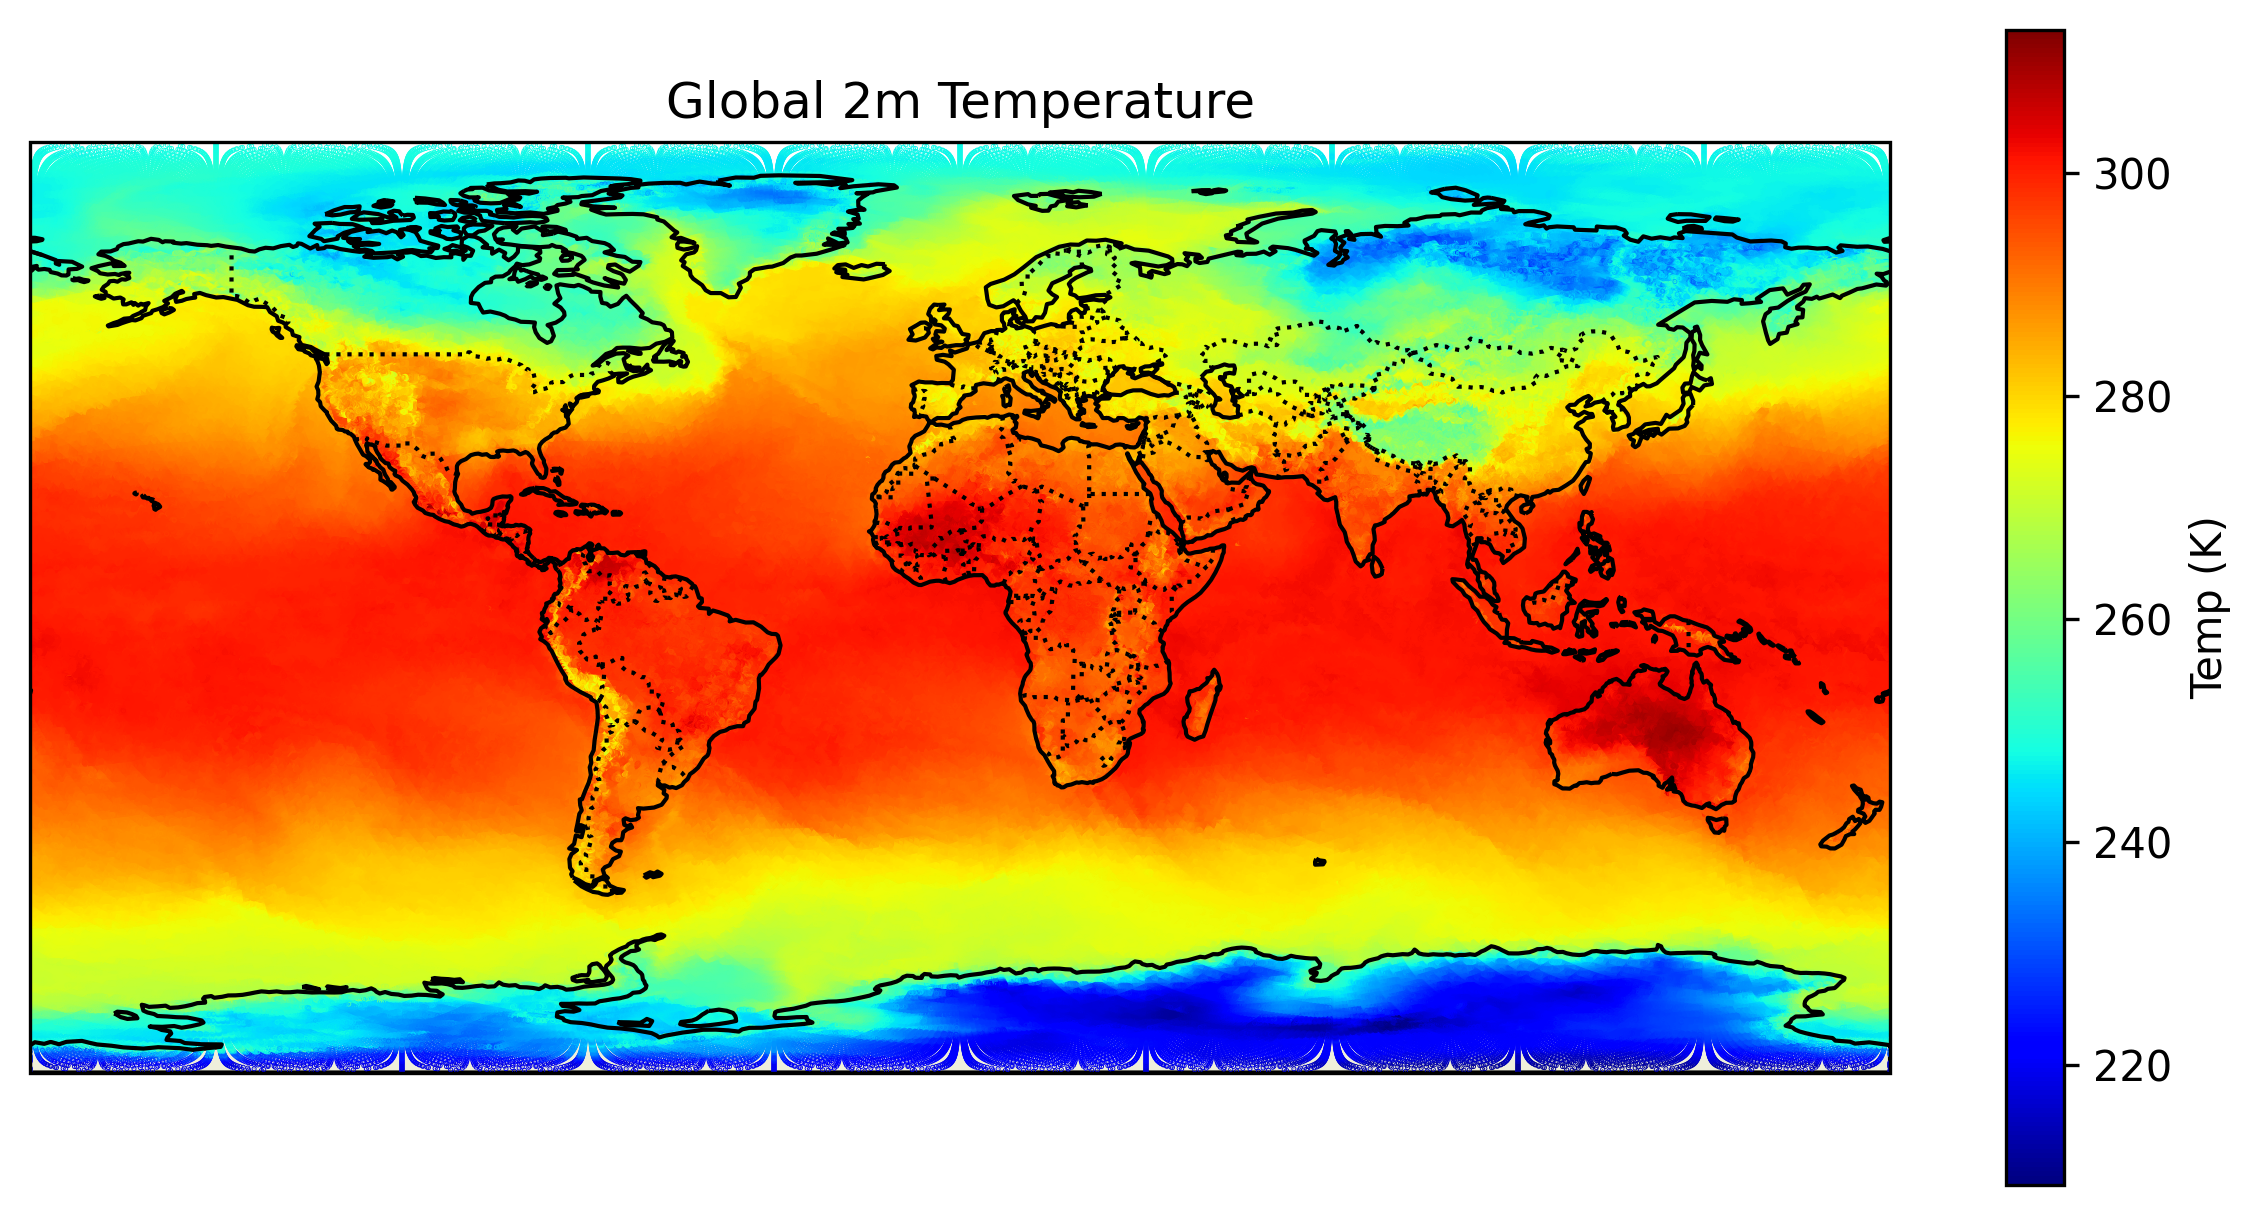
\includegraphics[width=\textwidth]{images/icon_t2m_global.png}
        \caption{Global 2m temperature field.}
        \label{fig:t2m_global_interp}
    \end{minipage}
    \hfill
    \begin{minipage}{0.4\textwidth}
        \centering
        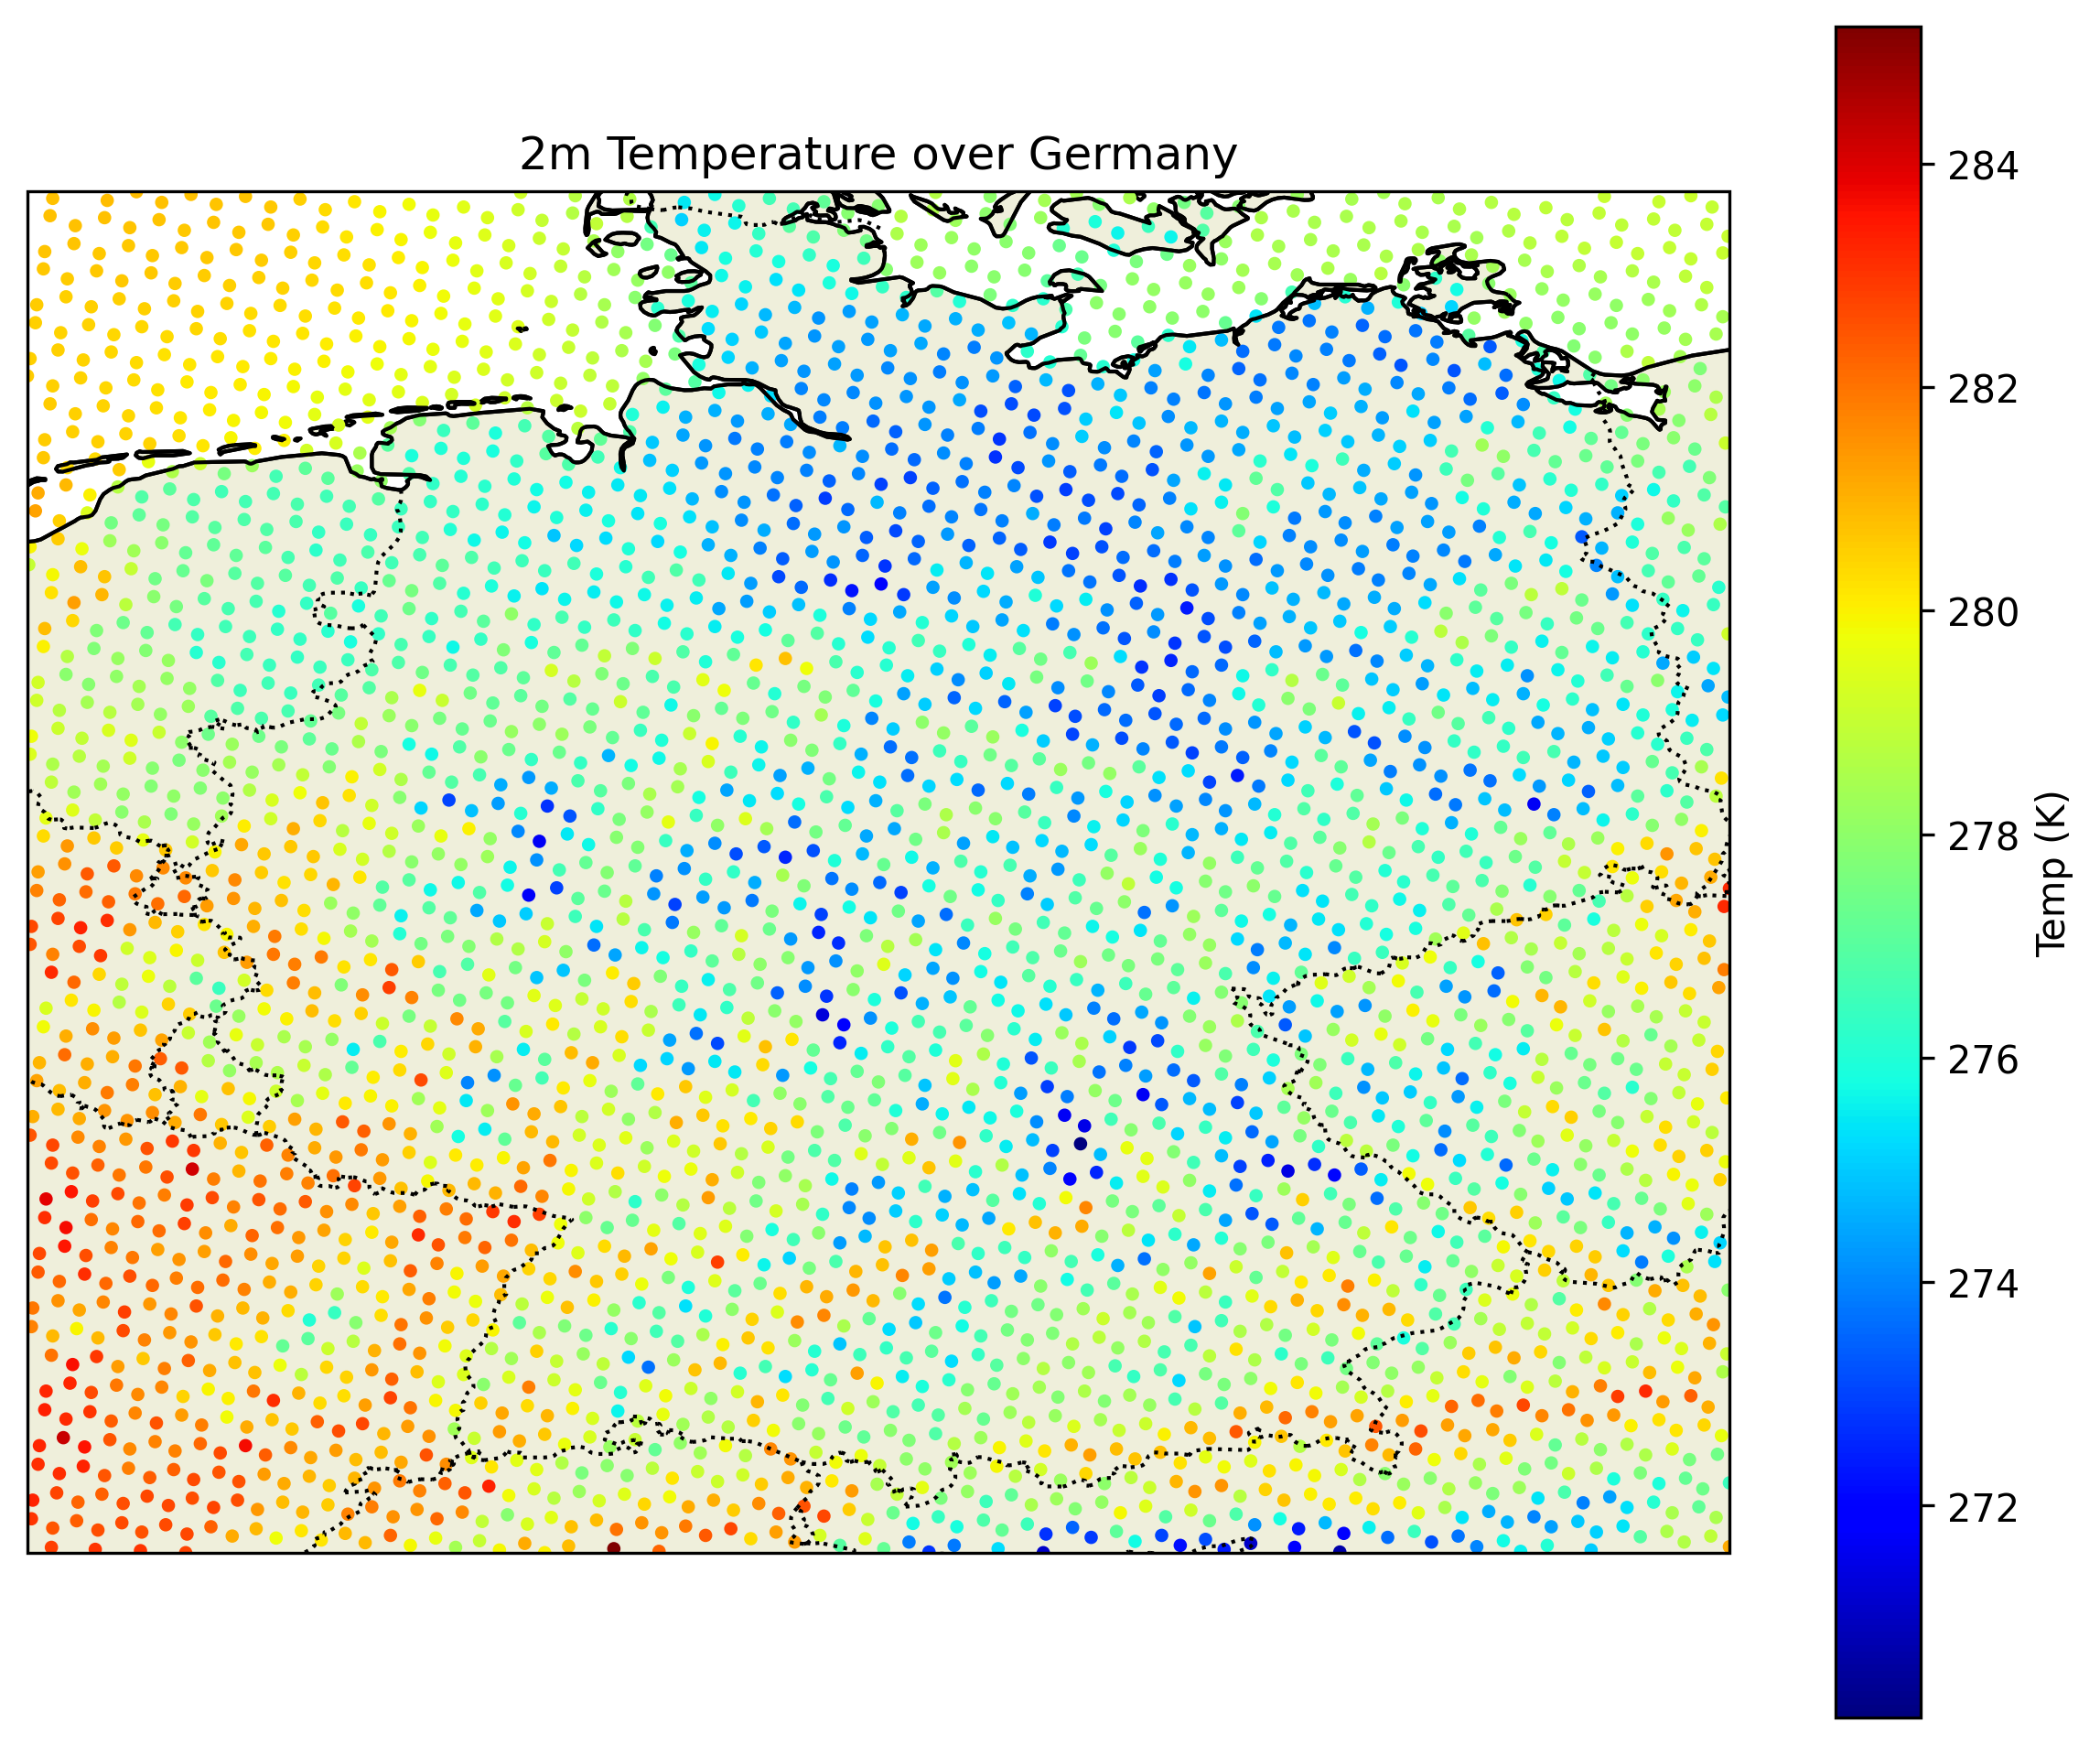
\includegraphics[width=\textwidth]{images/icon_t2m_germany.png}
        \caption{2m temperature field over Germany.}
        \label{fig:t2m_germany_interp}
    \end{minipage}
\end{figure}

\begin{figure}[ht]
    \centering
    \begin{minipage}{0.5\textwidth}
        \centering
        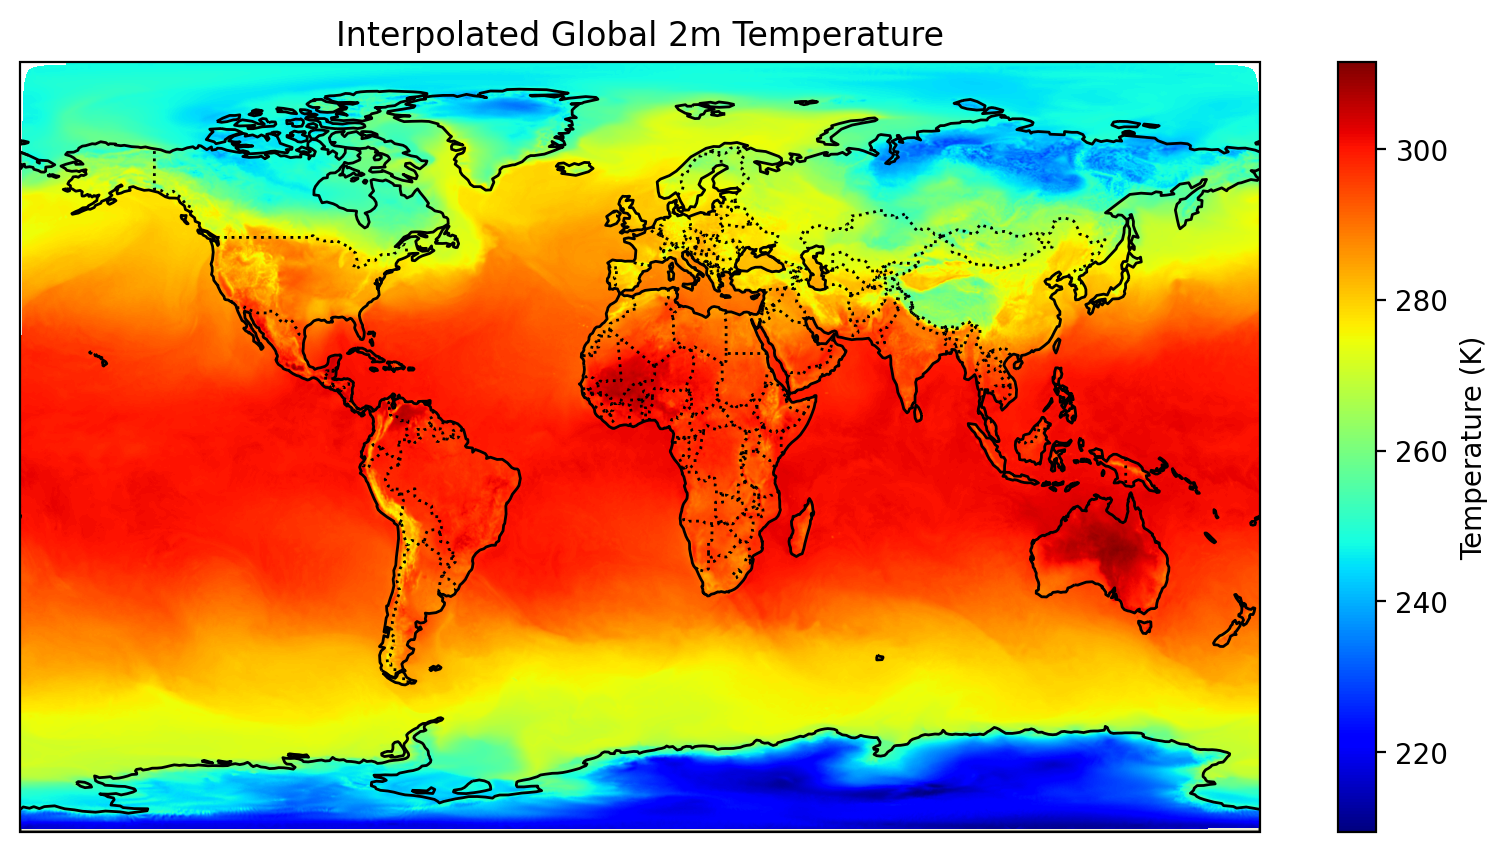
\includegraphics[width=\textwidth]{images/icon_t2m_global_interp.png}
        \caption{Interpolated global 2m temperature field.}
        \label{fig:t2m_global_interp}
    \end{minipage}
    \hfill
    \begin{minipage}{0.4\textwidth}
        \centering
        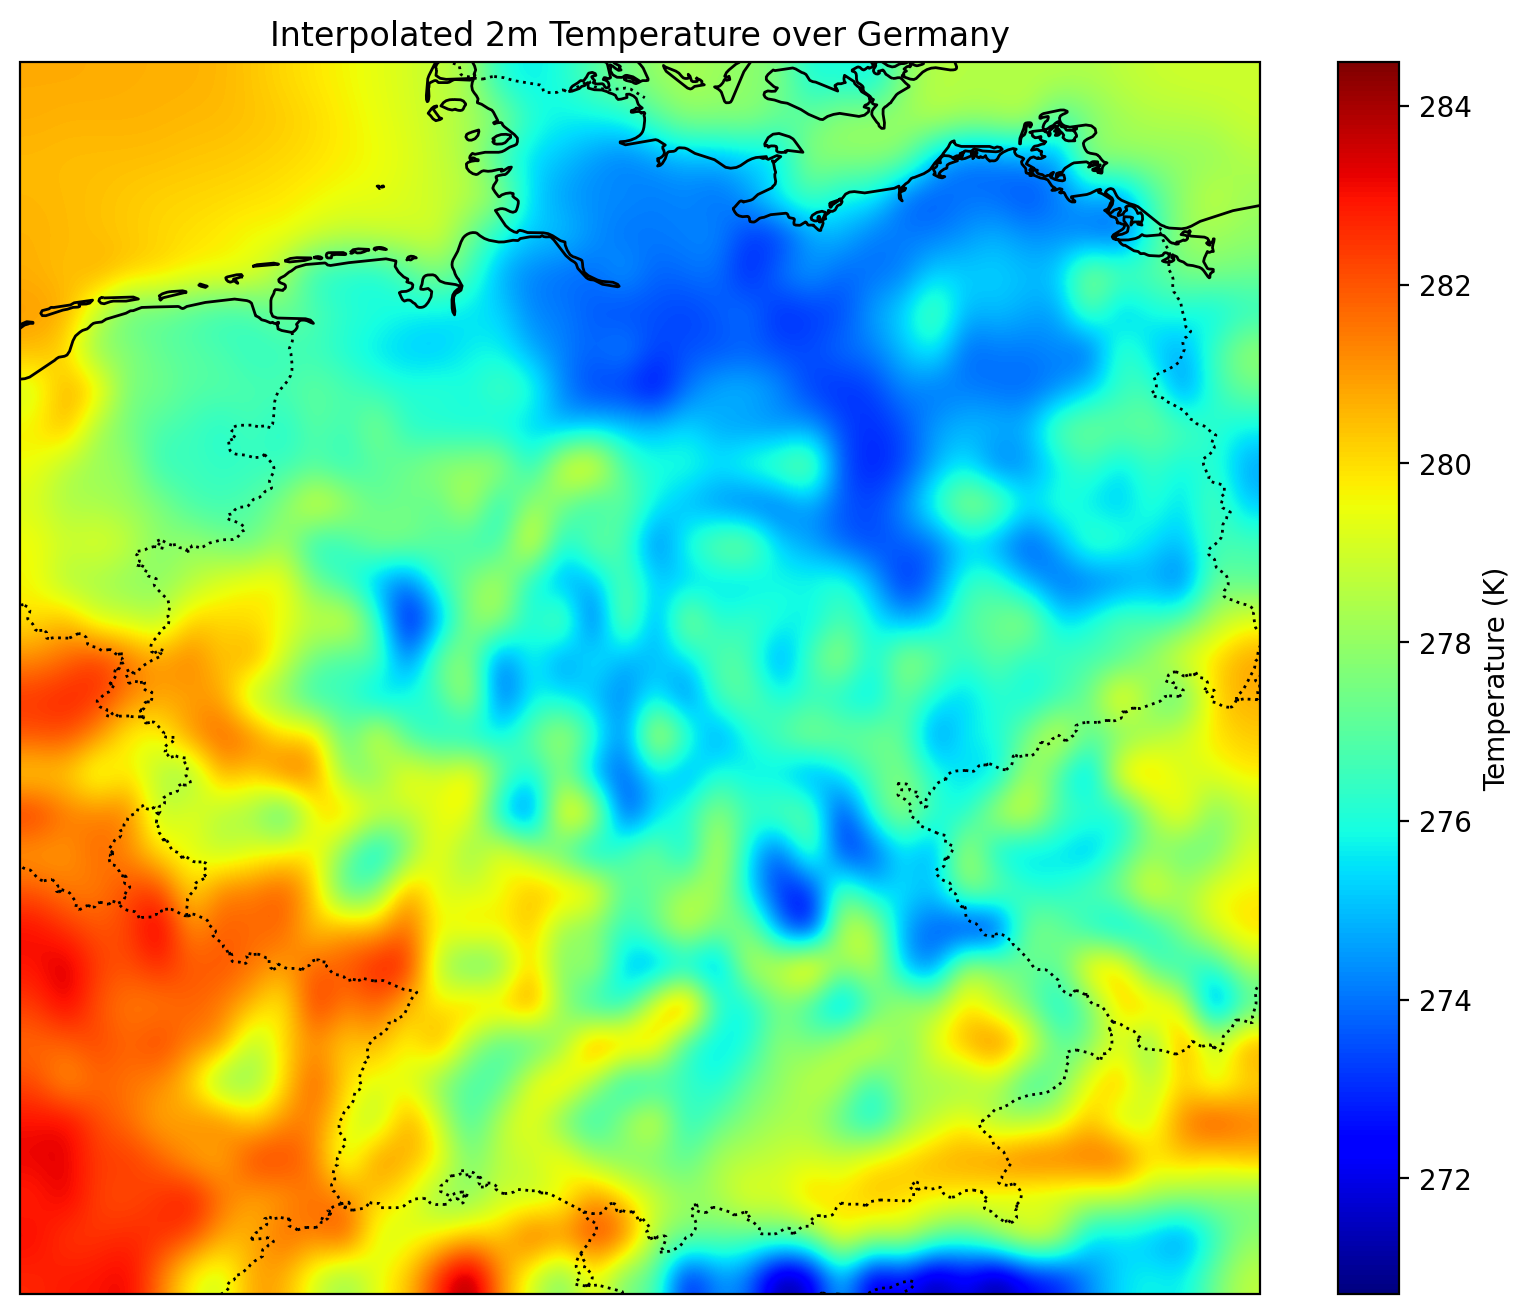
\includegraphics[width=\textwidth]{images/icon_t2m_germany_interp.png}
        \caption{Interpolated 2m temperature field over Germany.}
        \label{fig:t2m_germany_interp}
    \end{minipage}
\end{figure}

{\bf Interpolated Visualization of 2-Meter Temperature (T2M)}

To enhance the visualization of the 2-meter temperature field, we interpolate the scattered GRIB data onto a regular grid using cubic interpolation. This results in a smooth temperature field representation. The interpolation function is implemented as follows:

\begin{codeonly}{Interpolating T2M to a Regular Grid}
import numpy as np
from scipy.interpolate import griddata

def interpolate_to_grid(lat, lon, t2m, bbox, grid_res=0.25):
    """Interpolates T2M data onto a regular lat/lon grid."""
    latmin, latmax, lonmin, lonmax = bbox

    # Define a smooth regular grid
    grid_lat = np.arange(latmin, latmax, grid_res)
    grid_lon = np.arange(lonmin, lonmax, grid_res)
    lon_grid, lat_grid = np.meshgrid(grid_lon, grid_lat)

    # Use cubic interpolation for smooth output
    t2m_grid = griddata((lon, lat), t2m, (lon_grid, lat_grid), method='cubic')

    return lon_grid, lat_grid, t2m_grid
\end{codeonly}

Once the temperature field is interpolated, we visualize it using \texttt{matplotlib} and \texttt{cartopy}. The function for plotting the interpolated data is shown below:

\begin{codeonly}{Plotting Interpolated T2M}
import matplotlib.pyplot as plt
import cartopy.crs as ccrs
import cartopy.feature as cfeature

def plot_t2m_grid(lat, lon, t2m, bbox, title, fname):
    """Plots interpolated 2m temperature as a smooth heatmap."""
    lon_grid, lat_grid, t2m_grid = interpolate_to_grid(lat, lon, t2m, bbox)

    # Set reasonable aspect ratio based on bounding box size
    lon_range = bbox[3] - bbox[2]
    lat_range = bbox[1] - bbox[0]
    aspect_ratio = lon_range / lat_range
    figsize = (10, max(5, 10 / aspect_ratio))  # Maintain consistent width & prevent extreme height

    plt.figure(figsize=figsize)
    ax = plt.axes(projection=ccrs.PlateCarree())
    ax.set_extent([bbox[2], bbox[3], bbox[0], bbox[1]])
    ax.add_feature(cfeature.LAND, edgecolor='black')
    ax.add_feature(cfeature.COASTLINE)
    ax.add_feature(cfeature.BORDERS, linestyle=':')

    # Use smooth interpolation and correct aspect ratio
    img = ax.imshow(t2m_grid, extent=[bbox[2], bbox[3], bbox[0], bbox[1]], origin='lower',
                    cmap='jet', transform=ccrs.PlateCarree(), aspect='auto', interpolation='bicubic')

    plt.colorbar(img, label="Temperature (K)")
    plt.title(title)
    plt.savefig(fname, dpi=200, bbox_inches='tight')  # Reduce DPI for smaller file size
    plt.show()
\end{codeonly}

Using this interpolation approach, we generate the visualizations shown in Figures \ref{fig:t2m_global_interp} and \ref{fig:t2m_germany_interp} for the global and regional (Germany) temperature fields, see figure. 

\begin{recommendationbox}
Using libraries such as eccodes can be carried out in a very elementary way. At the same time, building packages is an important activity. Keep the balance, being able to do things elementary if necessary, while using packages to work efficiently. 
\end{recommendationbox}

%==============================================================================
%
%==============================================================================
\section{Accessing SYNOP Observation Files from NetCDF}

Observational weather data is often stored in the \emph{BUFR} (Binary Universal Form for the Representation of meteorological data) format, a widely used WMO standard. To facilitate data access, BUFR files are commonly converted into \emph{NetCDF} (Network Common Data Form), which provides a structured, self-describing format suitable for scientific applications.

NetCDF files containing SYNOP observations include essential meteorological variables such as temperature, pressure, humidity, wind speed, and cloud cover. Accessing these files requires a programming framework that can read NetCDF structures efficiently.

\begin{figure}[ht]
    \centering
    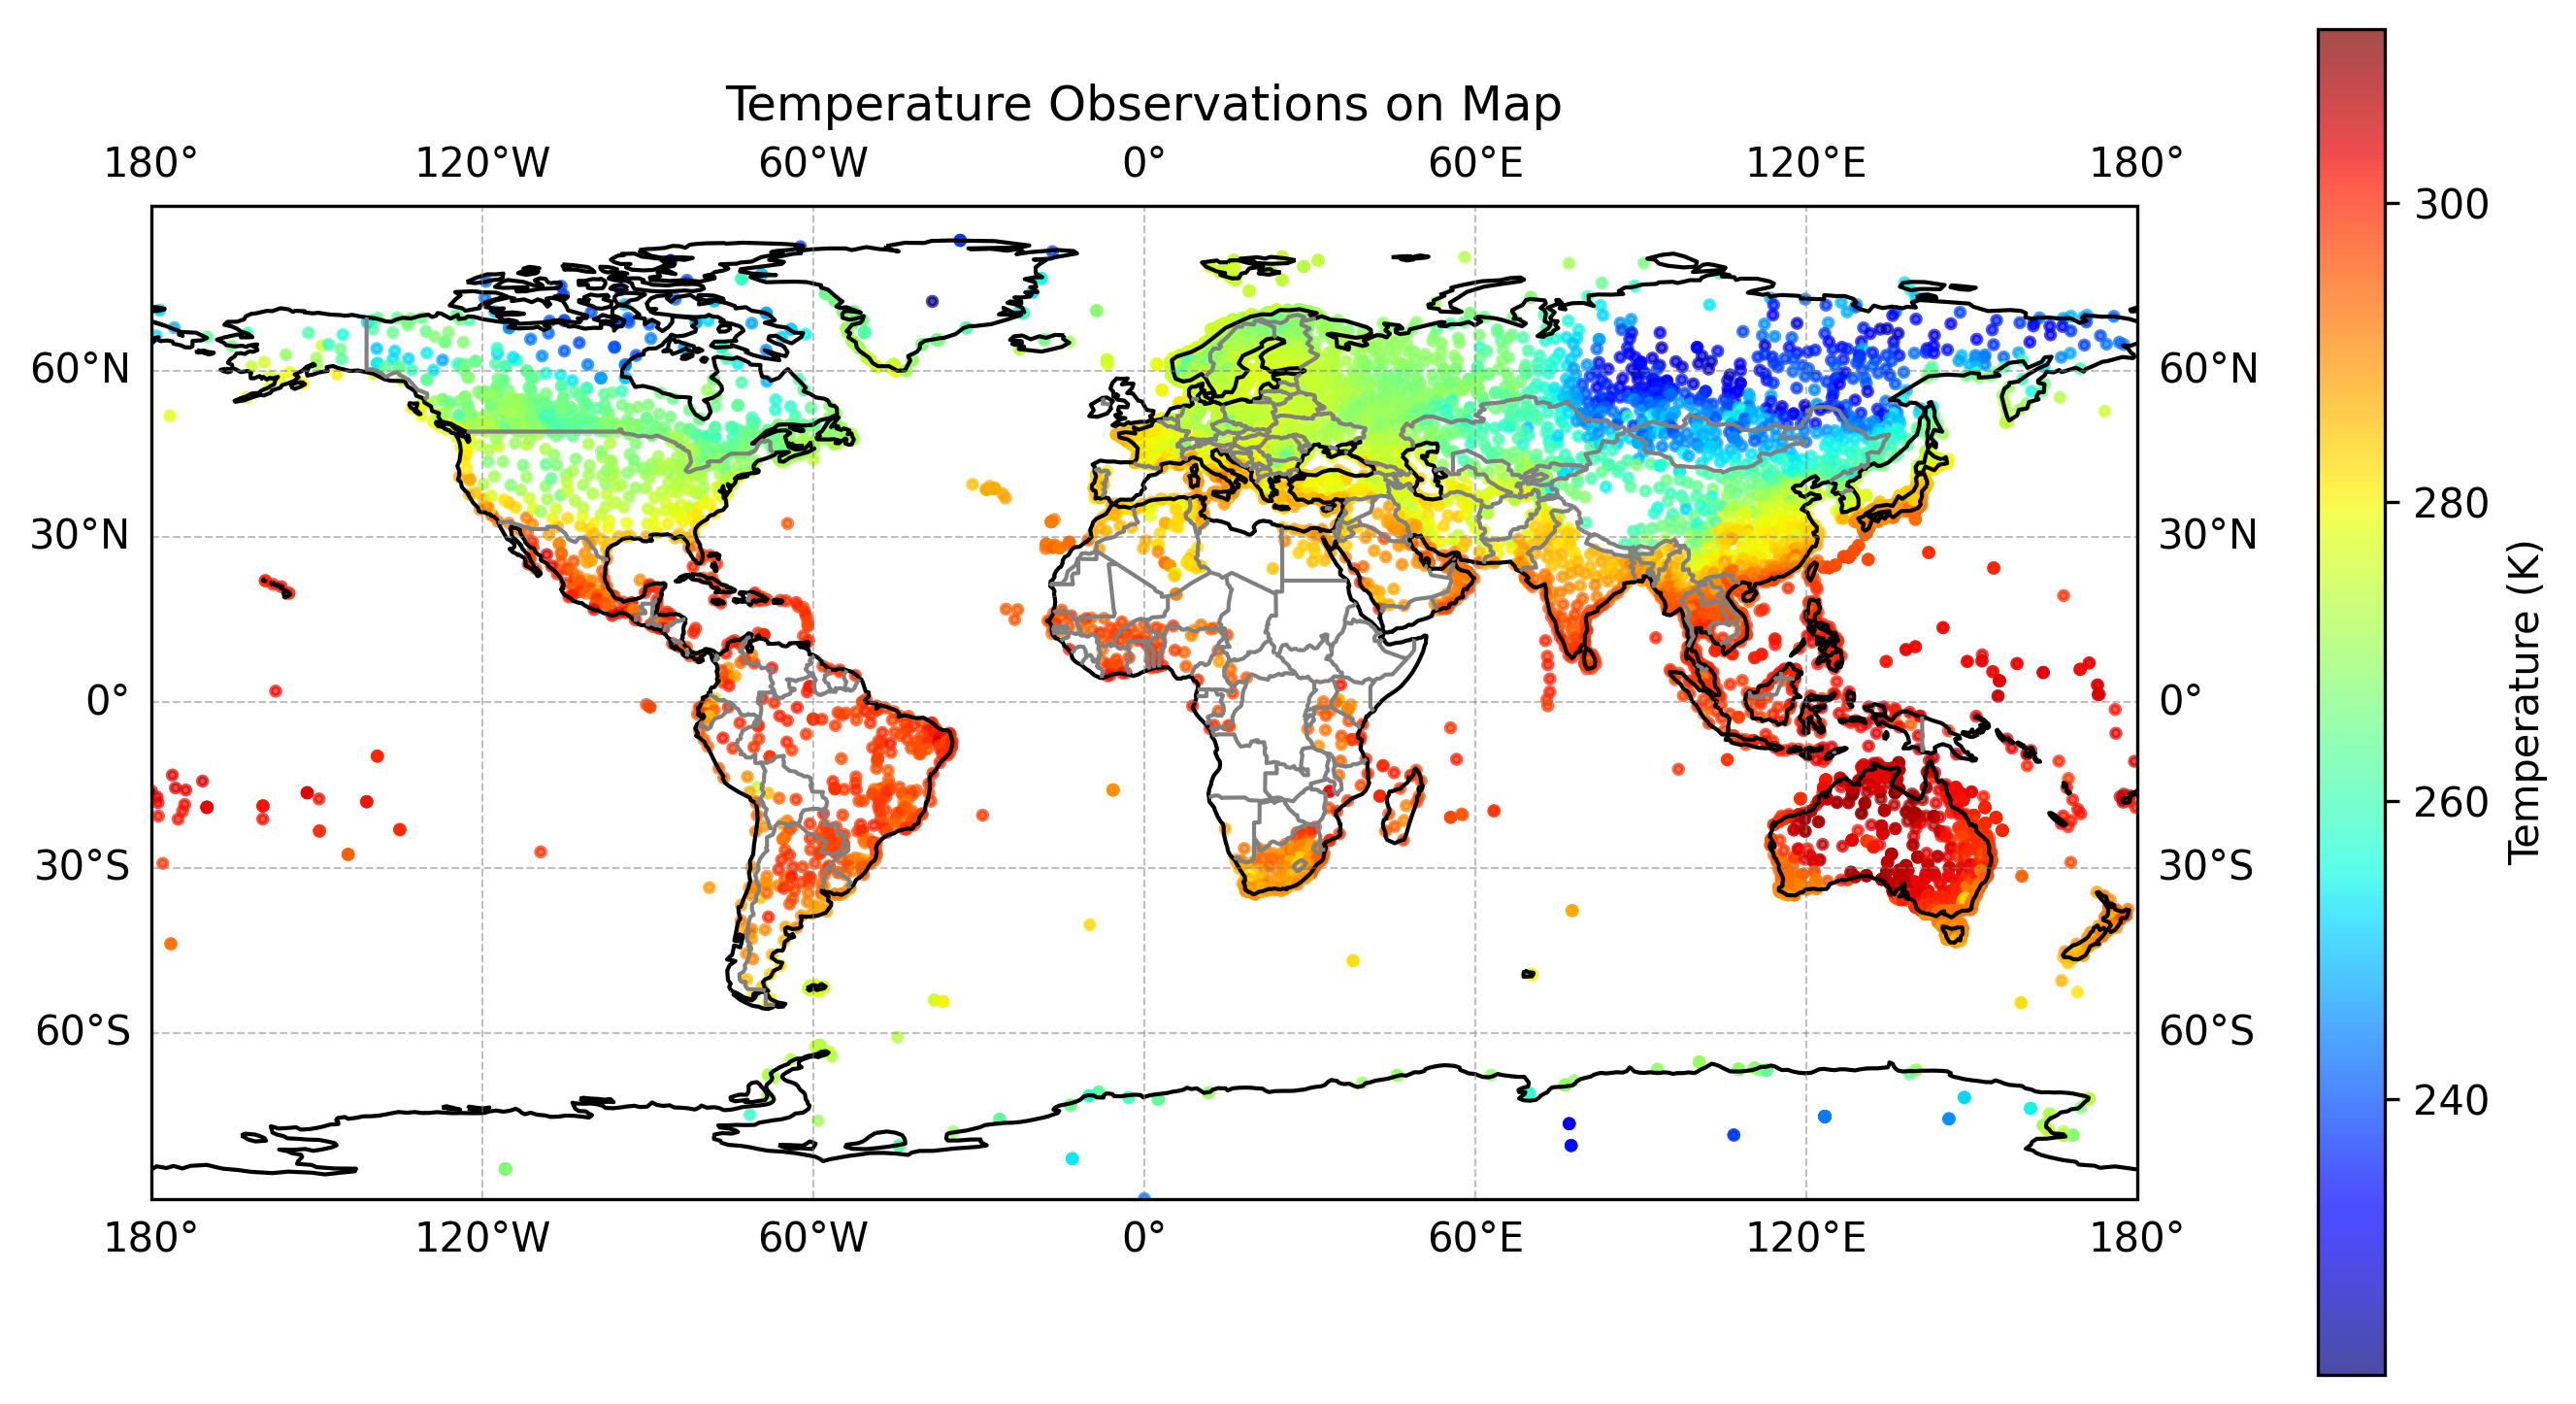
\includegraphics[width=0.9\textwidth]{images/synop.png}
    \caption{Scatter plot of SYNOP temperature observations}
    \label{fig:synop_plot}
\end{figure}

\textbf{Listing Variables in a NetCDF File}

To get an overview of the available variables, we use the following script:

\begin{codeonly}{Listing NetCDF Variables}
from netCDF4 import Dataset

def nc_list(file1):
    """
    Lists all variables in a given NetCDF file, displaying their names, dimensions, and descriptions.
    """
    ncfile = Dataset(file1, 'r')

    print("{:<4} {:40} {:>10} {:>10}  {:30}".format("No", "Varname", "shape1", "shape2", "Description"))
    print("-"*110)

    nc = 1
    for varname in ncfile.variables.keys():
        var = ncfile.variables[varname]
        description = var.long_name if hasattr(var, "long_name") else "N/A"
        dims = [len(ncfile.dimensions[dim]) for dim in var.dimensions]
        shape1 = dims[0] if len(dims) > 0 else ""
        shape2 = dims[1] if len(dims) > 1 else ""
        print("{:<4} {:40} {:>10} {:>10}  {:30}".format(nc, varname, shape1, shape2, description))  
        if nc % 10 == 0:
            print("-"*110)
        nc += 1
    ncfile.close()

file = "synop.nc"
nc_list(file)
\end{codeonly}

\textbf{Example Output}

\begin{codeonlysmall}{Example Output from nc\_list}
No   Varname                                      shape1     shape2  Description                   
--------------------------------------------------------------------------------------------------------------
1    edition_number                                11993             N/A                           
2    section1                                      11993         22  N/A                           
3    section2                                      11993         18  N/A                           
4    section1_master_table_nr                      11993             N/A                           
...
36   MLAH                                          11993             Latitude (high accuracy)      
37   MLOH                                          11993             Longitude (high accuracy)     
58   MTDBT                                         11993             Temperature/air temperature   
}
\end{codeonlysmall}

This function provides an overview of the variables, their dimensions, and descriptions if available, making it easier to understand the contents of the NetCDF file before further analysis.

\textbf{Frameworks for Accessing NetCDF Observations}

To work with SYNOP observations in NetCDF, we rely on established \emph{Python} libraries such as:
\begin{itemize}
    \item \texttt{netCDF4} -- Standard library for reading NetCDF data
    \item \texttt{numpy} -- Efficient numerical computations
    \item \texttt{matplotlib} -- Visualization of meteorological data
    \item \texttt{cartopy} -- Geospatial plotting on maps
\end{itemize}

\textbf{Reading SYNOP Data from NetCDF}

To extract observation data such as latitude, longitude, and temperature, we use the following Python script:

\begin{codeonly}{Reading latitude, longitude, and temperature from a NetCDF SYNOP file}
from netCDF4 import Dataset
import numpy as np

def read_synop_data(filename):
    """Reads latitude (MLAH), longitude (MLOH), and temperature (MTDBT) from a NetCDF file."""
    ncfile = Dataset(filename, 'r')
    
    lats = ncfile.variables["MLAH"][:]
    lons = ncfile.variables["MLOH"][:]
    temps = ncfile.variables["MTDBT"][:]
    
    ncfile.close()
    return np.array(lats), np.array(lons), np.array(temps)

# Example usage
lats, lons, temps = read_synop_data("synop.nc")
print("Latitudes:", lats[:5])
print("Longitudes:", lons[:5])
print("Temperatures:", temps[:5])
\end{codeonly}

\textbf{Filtering Missing Values}

NetCDF files contain default missing values, e.g., $9.96921\times10^{36}$. Before using the data, these values should be filtered out, here we employ a simple threshold:

\begin{codeonly}{Filtering large missing values in SYNOP NetCDF data}
def filter_missing_values(temps, threshold=1e+20):
    """Removes large default missing values from temperature data."""
    return temps[temps < threshold]

# Example usage
temps_filtered = filter_missing_values(temps)
\end{codeonly}

\textbf{Visualizing Observations on a Map}

For an intuitive representation of SYNOP data, we can plot temperature observations on a map:

\begin{codeonly}{Scatter plot of SYNOP temperature observations}
import numpy as np
import matplotlib.pyplot as plt
import cartopy.crs as ccrs
import cartopy.feature as cfeature

def plot_temperature_map(lats, lons, temps, filename="synop.png", threshold=1e+20):
    """Plots temperature observations on a map, removes large missing values, ensures proper colorbar spacing, and saves the figure."""

    # Filter out large missing values
    valid_mask = (temps < threshold) & np.isfinite(temps)
    lats, lons, temps = lats[valid_mask], lons[valid_mask], temps[valid_mask]

    # Create figure with proper aspect ratio
    fig, ax = plt.subplots(figsize=(10, 6), subplot_kw={'projection': ccrs.PlateCarree()})

    # Scatter plot with properly scaled colorbar
    scatter = ax.scatter(lons, lats, c=temps, cmap='coolwarm', s=5, alpha=0.7, transform=ccrs.PlateCarree())

    # Add map features
    ax.coastlines()
    ax.add_feature(cfeature.BORDERS, edgecolor='gray')
    ax.gridlines(draw_labels=True, linewidth=0.5, color='gray', alpha=0.5, linestyle='--')

    # Add colorbar with better spacing
    cbar = plt.colorbar(scatter, ax=ax, fraction=0.04, pad=0.08)
    cbar.set_label("Temperature (K)")

    # Set title
    plt.title("Temperature Observations on Map")

    # Save and show the plot
    plt.savefig(filename, dpi=300, bbox_inches="tight")
    plt.show()

# Example usage
plot_temperature_map(lats, lons, temps)
\end{codeonly}

This script generates a scatter plot where each SYNOP observation is plotted on a geographical map, see Figure \ref{fig:synop_plot}. The color of each point represents the observed temperature, providing a clear spatial overview of meteorological conditions.


%==============================================================================
%
%==============================================================================
\section{Analysing AIREP Feedback Files in NetCDF Format}

Aircraft Reports (AIREP) provide vital meteorological observations from airborne sources. These reports contain real-time measurements of parameters such as temperature, wind speed, pressure, and humidity. The data is often stored in \emph{BUFR} (Binary Universal Form for the Representation of meteorological data) format and later converted into \emph{NetCDF} (Network Common Data Form) for easier access and processing.

\textbf{Structure of AIREP NetCDF Files}

AIREP feedback files in NetCDF format consist of multiple dimensions and variables. The primary dimensions include:

\begin{itemize}
    \item \texttt{d\_hdr} -- Number of header entries (stations, timestamps, metadata)
    \item \texttt{d\_body} -- Number of observed variables (measurements at different levels)
    \item \texttt{d\_veri} -- Number of verification entries
\end{itemize}

Each observation is associated with key metadata, including:

\begin{itemize}
    \item \texttt{lat}, \texttt{lon} -- Geographic coordinates of the observation
    \item \texttt{varno} -- Variable number defining the type of measurement
    \item \texttt{obs} -- Observed value, bias-corrected
    \item \texttt{plevel} -- Pressure level at which the observation was made
    \item \texttt{veri\_data} -- Corresponding modeled values for verification
\end{itemize}

\textbf{Inspecting Variables in AIREP NetCDF Files}

To get an overview of the available variables, the following Python function lists all variables along with their dimensions and descriptions:

\begin{codeonly}{Listing NetCDF Variables in AIREP Files}
from netCDF4 import Dataset

def nc_list(file1):
    """
    Lists all variables in a given NetCDF file, displaying their names, dimensions, and descriptions.
    
    Parameters:
    file1 (str): Path to the NetCDF file.

    Output:
    Prints a formatted table of variables with their dimensions and descriptions.
    """
    ncfile = Dataset(file1, 'r')

    print("{:<4} {:40} {:>10} {:>10}  {:30}".format("No", "Varname", "shape1", "shape2", "Description")) 
    print("-" * 110)

    nc = 1
    for varname in ncfile.variables.keys():
        var = ncfile.variables[varname]
        
        # Retrieve description from correct attribute
        description = getattr(var, "longname", "N/A")

        # Get variable dimensions
        dims = [len(ncfile.dimensions[dim]) for dim in var.dimensions]

        # Ensure at least 2 shape values
        shape1 = dims[0] if len(dims) > 0 else ""
        shape2 = dims[1] if len(dims) > 1 else ""

        print("{:<4} {:40} {:>10} {:>10}  {:30}".format(nc, varname, shape1, shape2, description))

        if nc % 10 == 0: 
            print("-" * 110)
        nc += 1

    ncfile.close()

# Example usage
file = "monAIREP.nc"
nc_list(file)
\end{codeonly}

\begin{codeonlysmall}{Example Output of nc\_list}
No   Varname                       shape1     shape2  Description                   
----------------------------------------------------------------------------------------------------
1    i_body                         37198             index of 1st entry in report body
2    l_body                         37198             number of entries in report body
3    n_level                        37198             number of levels in report    
4    data_category                  37198             BUFR4 data category           
5    sub_category                   37198             BUFR4 data sub-category       
6    center                         37198             station processing center     
7    sub_center                     37198             station processing sub-center 
8    obstype                        37198             observation type              
9    codetype                       37198             code type                     
10   ident                          37198             station or satellite id as integer
----------------------------------------------------------------------------------------------------
11   statid                         37198         10  station id as character string
12   lat                            37198             latitude                      
13   lon                            37198             longitude                     
14   time                           37198             observation minus reference time
15   time_nomi                      37198             nominal (synoptic) minus reference time
16   time_dbase                     37198             data base minus reference time
17   z_station                      37198             station height                
18   z_modsurf                      37198             model surface height          
19   r_state                        37198             status of the report          
20   r_flags                        37198             report quality check flags    
----------------------------------------------------------------------------------------------------
21   r_check                        37198             check which raised the report status flag value
22   sta_corr                       37198             station correction indicator  
23   index_x                        37198             index x of model grid point assigned to report
24   index_y                        37198             index y of model grid point assigned to report
25   mdlsfc                         37198             model surface characteristics 
26   instype                        37198             station type or satellite instrument type
27   sun_zenit                      37198             sun zenith angle              
28   phase                          37198             aircraft phase                
29   tracking                       37198             tracking technique            
30   obs_id                         37198             unique observation id         
----------------------------------------------------------------------------------------------------
31   source                         37198             input file number             
32   record                         37198             record number in the input file
33   subset                         37198             subset number in the record   
34   dbkz                           37198             DWD data base id              
35   index_d                        37198             model grid diamond index assigned to report
36   varno                         187770             type of the observed quantity 
37   obs                           187770             bias corrected observation    
38   bcor                          187770             bias correction, corrected minus observed
39   level                         187770             level of observation          
40   level_typ                     187770             type of level information     
----------------------------------------------------------------------------------------------------
41   level_sig                     187770             level significance            
42   state                         187770             status of the observation     
43   flags                         187770             observation quality check flags
44   check                         187770             check which raised the observation status flag value
45   e_o                           187770             observational error           
46   qual                          187770             observation confidence from data provider
47   plevel                        187770             nominal pressure level        
48   veri_data                          5     187770  modelled quantity (as indicated by veri_ens_member)
49   veri_model                         5         10  model used for verification, e.g. COSMO, GME ...
50   veri_run_type                      5             type of model run             
----------------------------------------------------------------------------------------------------
51   veri_run_class                     5             class of model run            
...
\end{codeonlysmall}

\textbf{Extracting AIREP Observations from NetCDF}

To retrieve latitude, longitude, and observation values, we use the following function:

\begin{codeonly}{Reading AIREP Observations from NetCDF}
from netCDF4 import Dataset
import numpy as np
import matplotlib.pyplot as plt
import cartopy.crs as ccrs
import cartopy.feature as cfeature

def read_airep_data(filename, varno, extra_vars=None):
    """Reads latitude, longitude, selected observations, and additional variables from a NetCDF file."""
    if extra_vars is None:
        extra_vars = []

    ncfile = Dataset(filename, 'r')
    
    # Read header-level variables
    lat = ncfile.variables["lat"][:]
    lon = ncfile.variables["lon"][:]
    
    # Read body-level variables
    varno_all = ncfile.variables["varno"][:]
    obs_all = ncfile.variables["obs"][:]
    l_body = ncfile.variables["l_body"][:]

    # Expand lat/lon to match body-level observations
    ni = len(l_body)
    ie = np.repeat(range(0, ni), l_body)
    
    # Find matching variable numbers
    idx = np.where(varno_all == varno)[0]
    
    # Filter lat, lon, obs
    lat_filtered = lat[ie[idx]]
    lon_filtered = lon[ie[idx]]
    obs_filtered = obs_all[idx]

    # Read extra variables if requested
    extra_data = {}
    for var in extra_vars:
        if var in ncfile.variables:
            var_data = ncfile.variables[var][:]
            extra_data[var] = var_data[idx] if var_data.shape[0] == len(varno_all) else var_data[ie[idx]]
        else:
            print(f"Warning: Variable '{var}' not found in NetCDF file.")

    ncfile.close()
    return lat_filtered, lon_filtered, obs_filtered, extra_data

\end{codeonly}

\begin{figure}[ht]
    \centering
    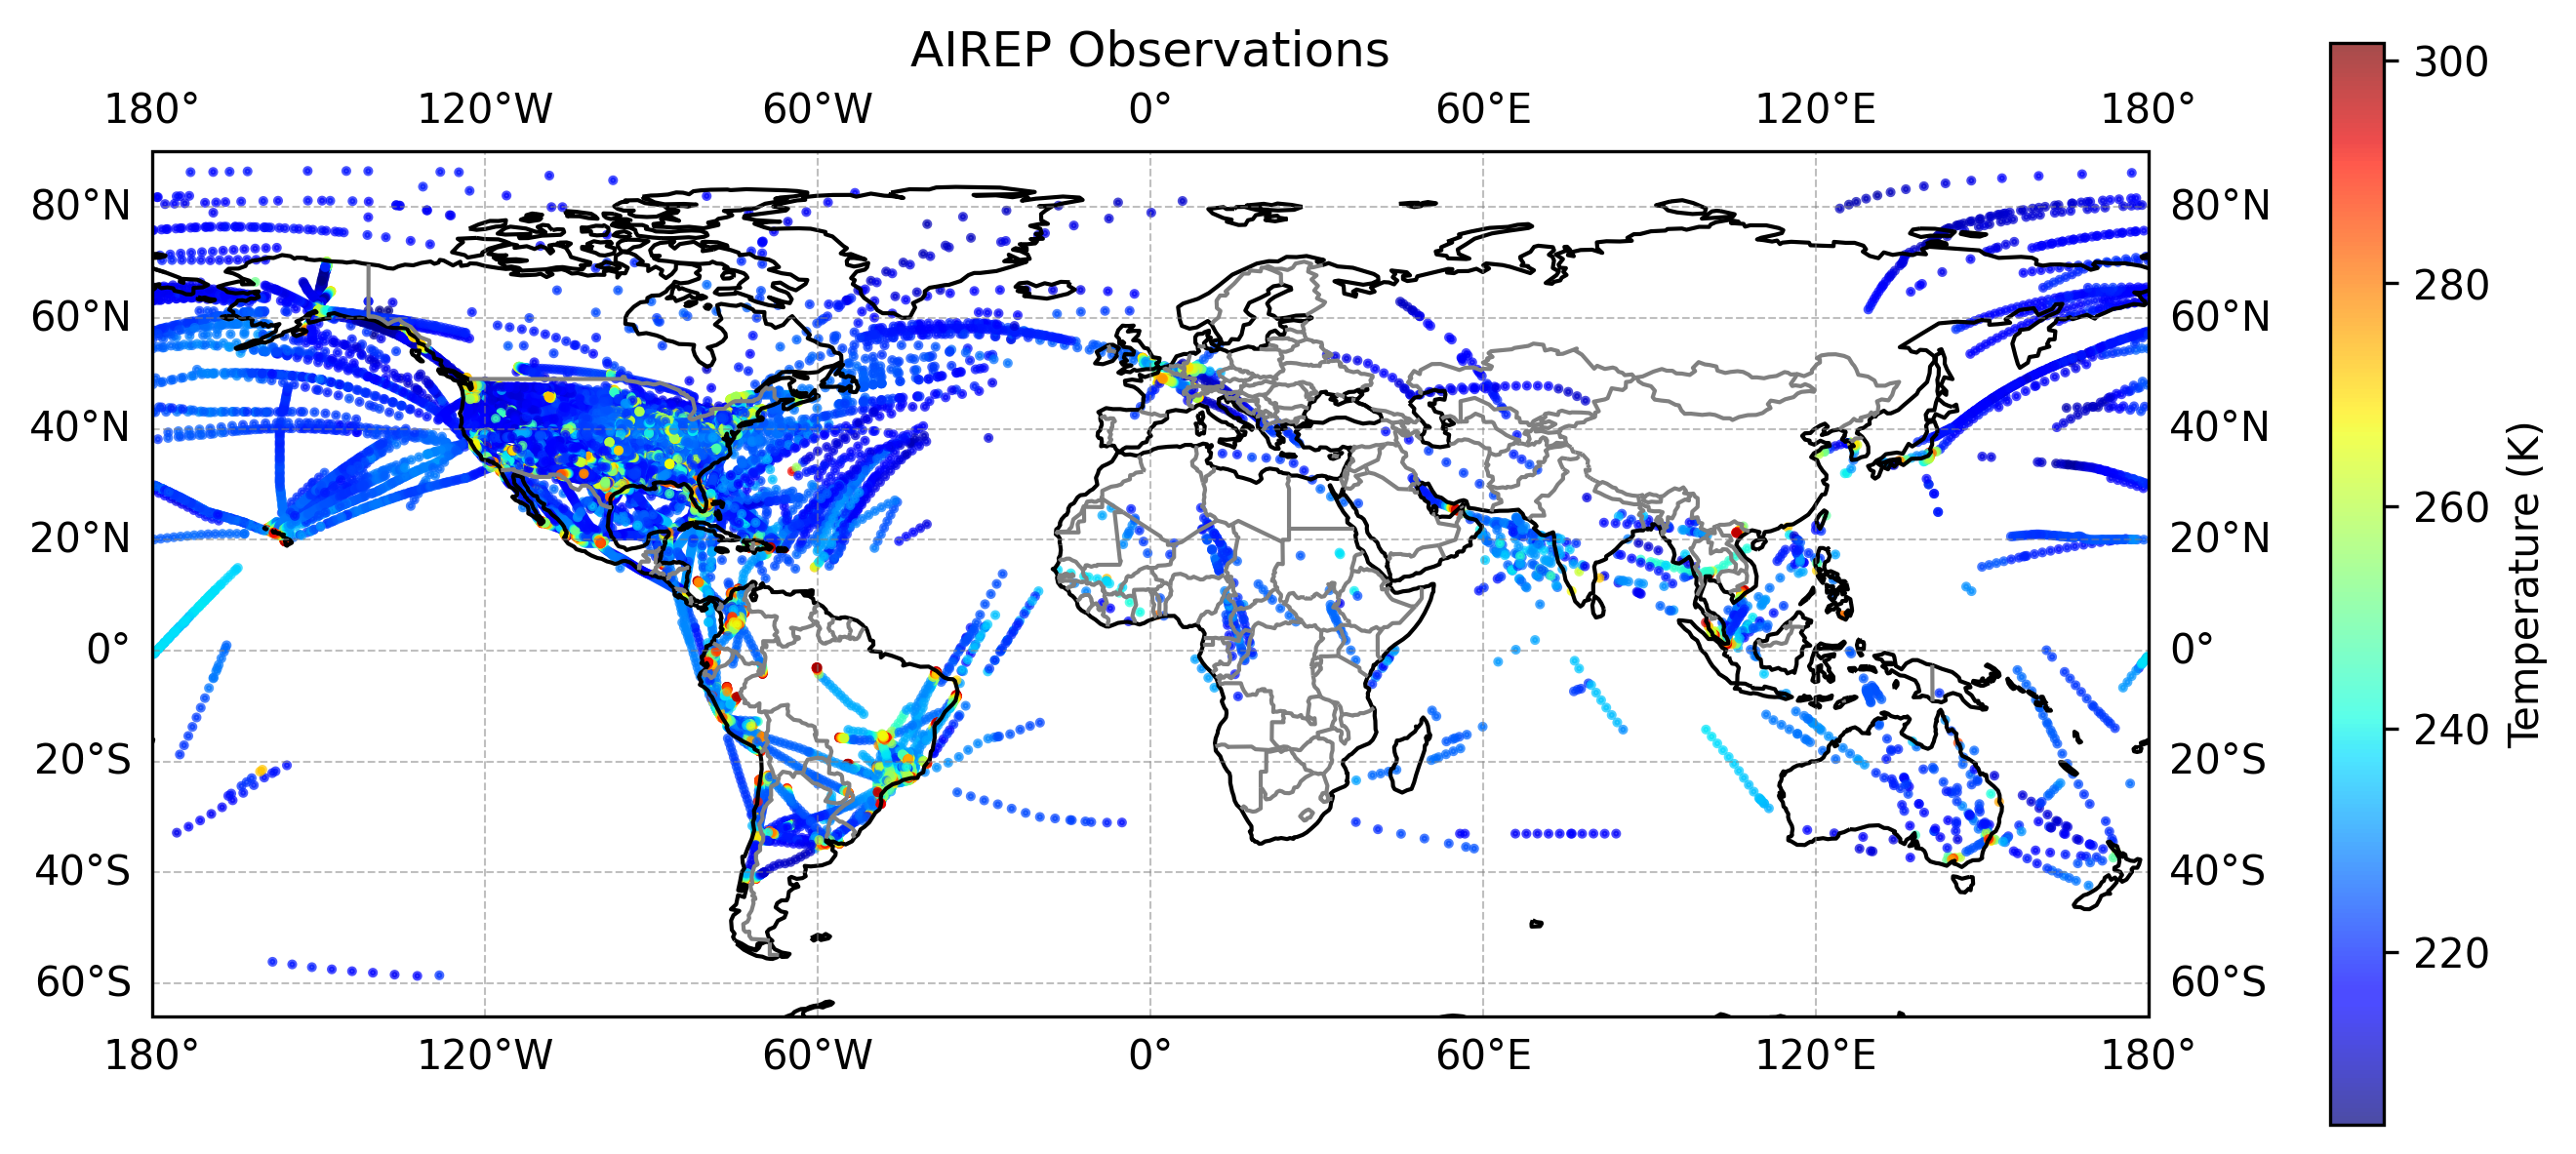
\includegraphics[width=0.9\textwidth]{images/airep.png}
    \caption{Scatter plot of AIREP observations}
    \label{fig:airep_plot}
\end{figure}

\textbf{Filtering Out Missing Values and Outliers}

AIREP NetCDF files may contain default missing values (e.g., $9.96921\times10^{36}$) and unrealistic outliers. We filter them as follows:

\begin{codeonly}{Filtering Missing Values and Outliers in AIREP Data}
def filter_airep_data(lats, lons, obs, threshold=1e+20):
    """Filters AIREP observations by removing missing values and out-of-range temperatures."""
    valid_mask = (obs < threshold) & np.isfinite(obs)
    lats, lons, obs = lats[valid_mask], lons[valid_mask], obs[valid_mask]
    temp_min, temp_max = 180, 320
    physical_mask = (obs >= temp_min) & (obs <= temp_max)
    return lats[physical_mask], lons[physical_mask], obs[physical_mask]
\end{codeonly}

\textbf{Visualizing AIREP Observations on a Map}

For a better understanding of the spatial distribution of AIREP observations, we plot them on a map using the following function:

\begin{codeonly}{Plotting AIREP Observations on a Map}
def plot_airep_map(lats, lons, obs, filename="airep.png"):
    """Plots AIREP observations on a map after filtering out-of-range temperatures."""

    fig, ax = plt.subplots(figsize=(10, 6), subplot_kw={'projection': ccrs.PlateCarree()})

    scatter = ax.scatter(lons, lats, c=obs, cmap='jet', s=2, alpha=0.7, transform=ccrs.PlateCarree())

    ax.coastlines()
    ax.add_feature(cfeature.BORDERS, edgecolor='gray')
    ax.gridlines(draw_labels=True, linewidth=0.5, color='gray', alpha=0.5, linestyle='--')

    # Ensure the colorbar does not exceed figure height
    cbar = fig.colorbar(scatter, ax=ax, orientation='vertical', fraction=0.04, pad=0.08, shrink=0.8)
    cbar.set_label("Temperature (K)")

    plt.title("AIREP Observations")
    plt.savefig(filename, dpi=300, bbox_inches="tight")
    plt.show()

# Example usage
lats_filtered, lons_filtered, obs_filtered = filter_airep_data(lats, lons, obs)
plot_airep_map(lats_filtered, lons_filtered, obs_filtered)
\end{codeonly}


The visualization of Figure \ref{fig:airep_plot} allows for a quick assessment of the coverage and accuracy of aircraft-derived meteorological data.

\begin{figure}[ht]
    \centering
    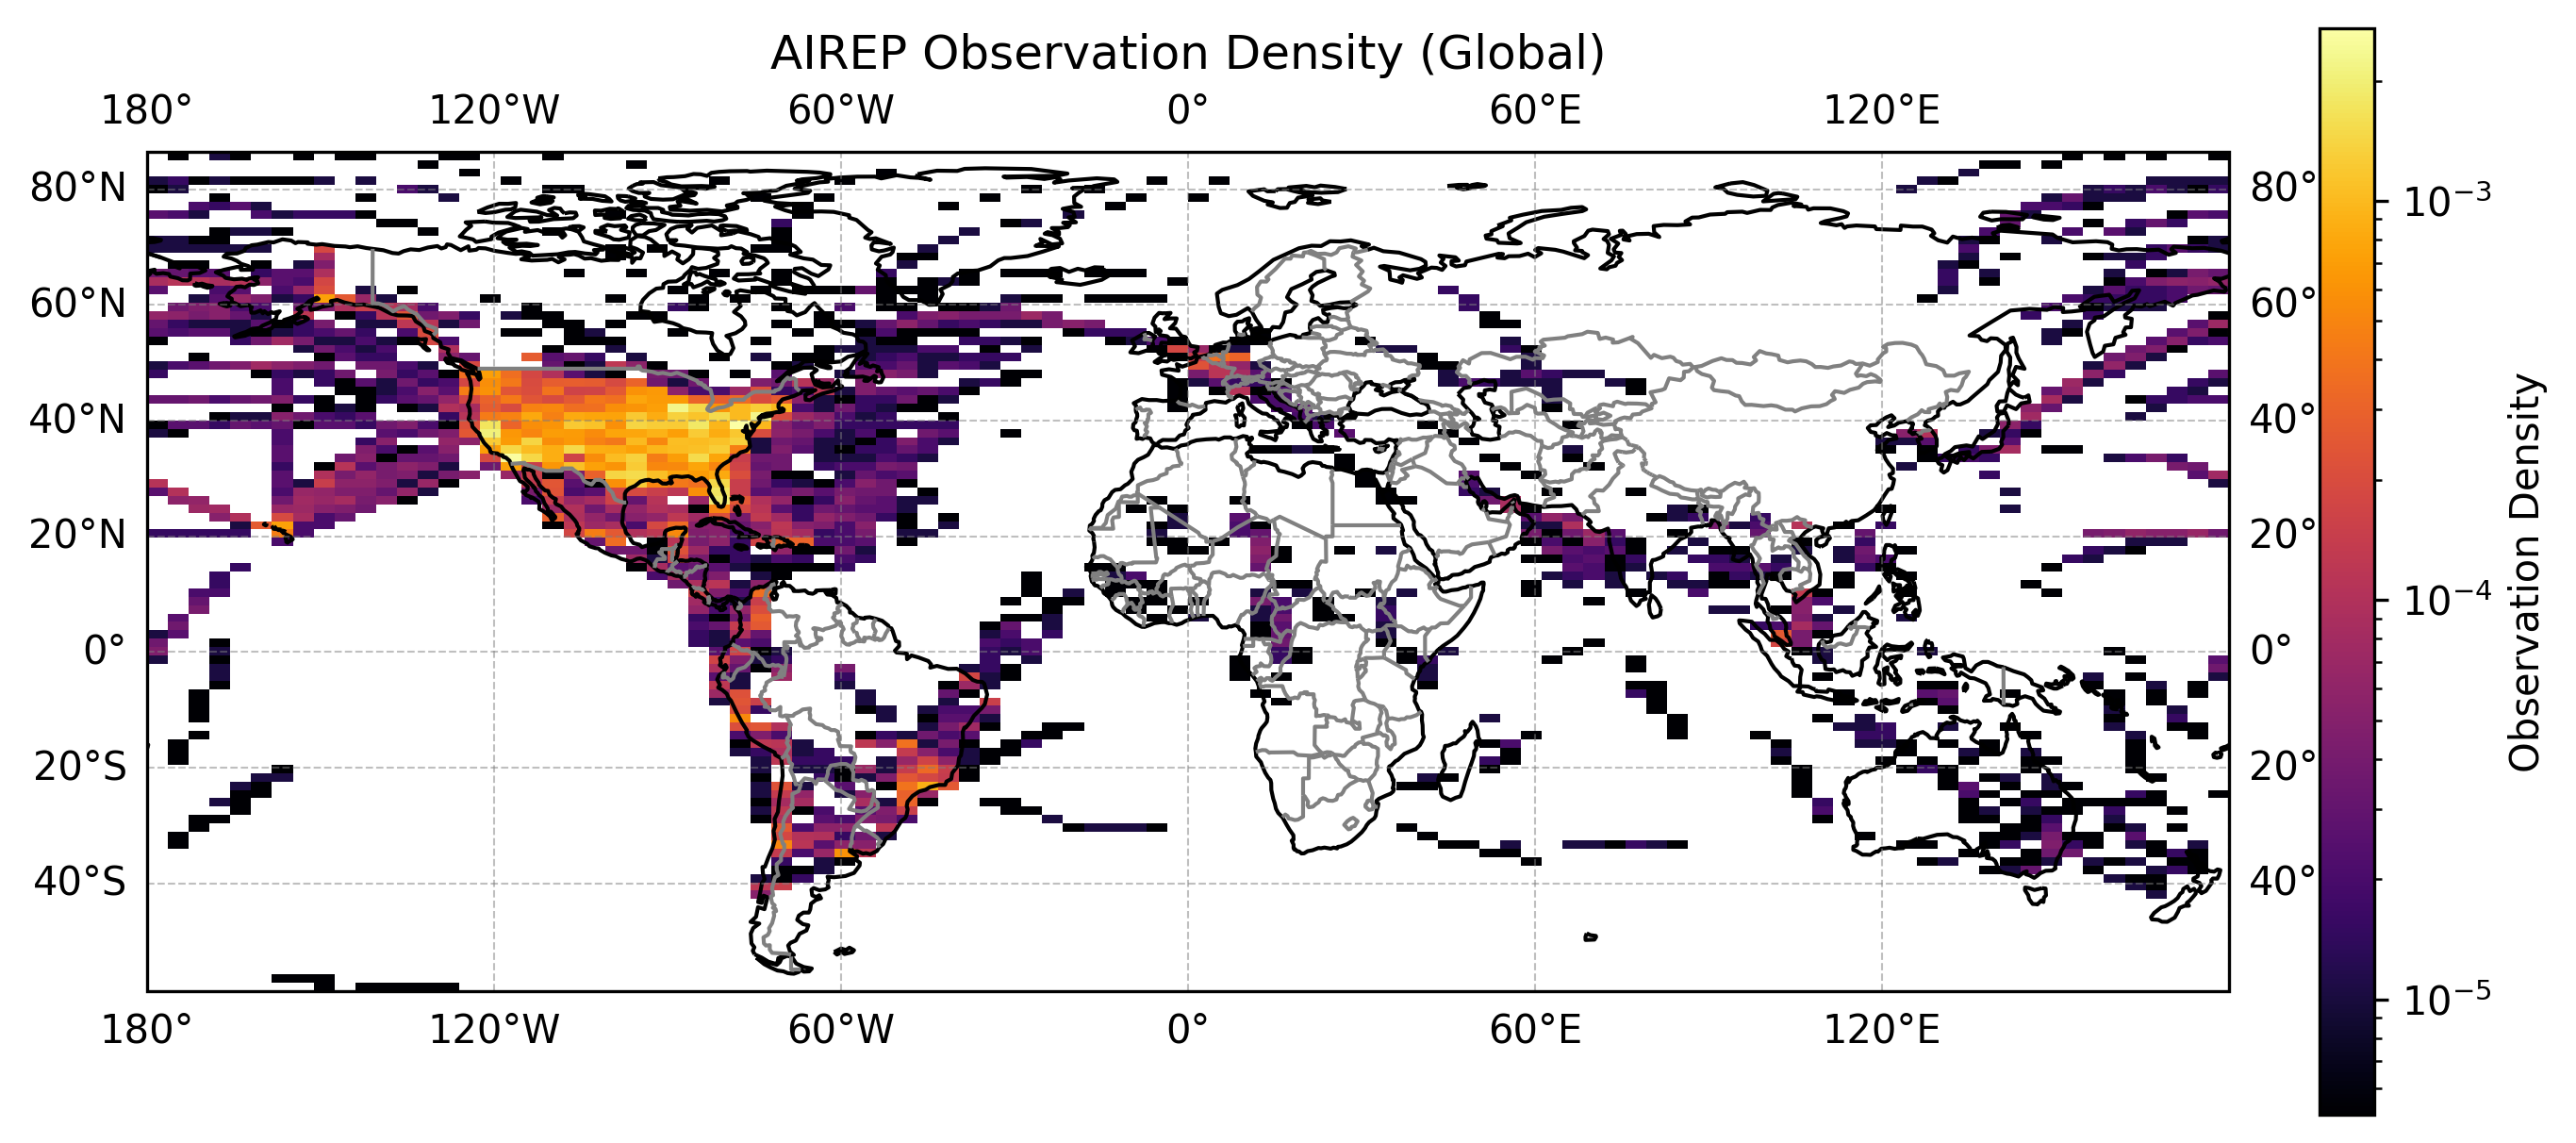
\includegraphics[width=0.9\textwidth]{images/airep_global_density.png}
    \caption{AIREP density in its horizontal distribution, while daytime in the US.}
    \label{fig:airep_plot}
\end{figure}


We can now analyse these data, for example by visualization of measurement density in horizontal or vertical distribution. 

\begin{codeonly}{Global AIREP Density Visualization}
import matplotlib.pyplot as plt
import cartopy.crs as ccrs
import cartopy.feature as cfeature
import numpy as np
from scipy.stats import gaussian_kde
from netCDF4 import Dataset

def plot_global_density(lats, lons,
                        filename="airep_global_density.png"):
    """Generates a density plot of AIREP observations on a world map 
    with an optimized colormap."""
    fig, ax = plt.subplots(figsize=(10, 6),
                           subplot_kw={'projection': ccrs.PlateCarree()})
    
    # Compute 2D histogram
    hist, xedges, yedges = np.histogram2d(lons, lats,
                                          bins=100, density=True)
    
    # Use a perceptually uniform colormap (e.g., 'inferno')
    pcm = ax.pcolormesh(xedges, yedges, hist.T, cmap='inferno',
                        norm=plt.matplotlib.colors.LogNorm(
                            vmin=hist[hist > 0].min(),
                            vmax=hist.max()),
                        transform=ccrs.PlateCarree())
    
    ax.coastlines()
    ax.add_feature(cfeature.BORDERS, edgecolor='gray')
    ax.gridlines(draw_labels=True, linewidth=0.5,
                 color='gray', alpha=0.5, linestyle='--')
    
    # Adjust padding to ensure axis does not crowd the figure
    plt.subplots_adjust(left=0.1, right=0.9, top=0.9, bottom=0.1)
    
    # Ensure colorbar does not exceed figure size
    cbar = fig.colorbar(pcm, ax=ax, orientation='vertical',
                        fraction=0.04, pad=0.04, shrink=0.8)
    cbar.set_label("Observation Density")
    
    plt.title("AIREP Observation Density (Global)")
    plt.savefig(filename, dpi=300, bbox_inches="tight")
    plt.show()
\end{codeonly}


\begin{figure}[ht]
    \centering
    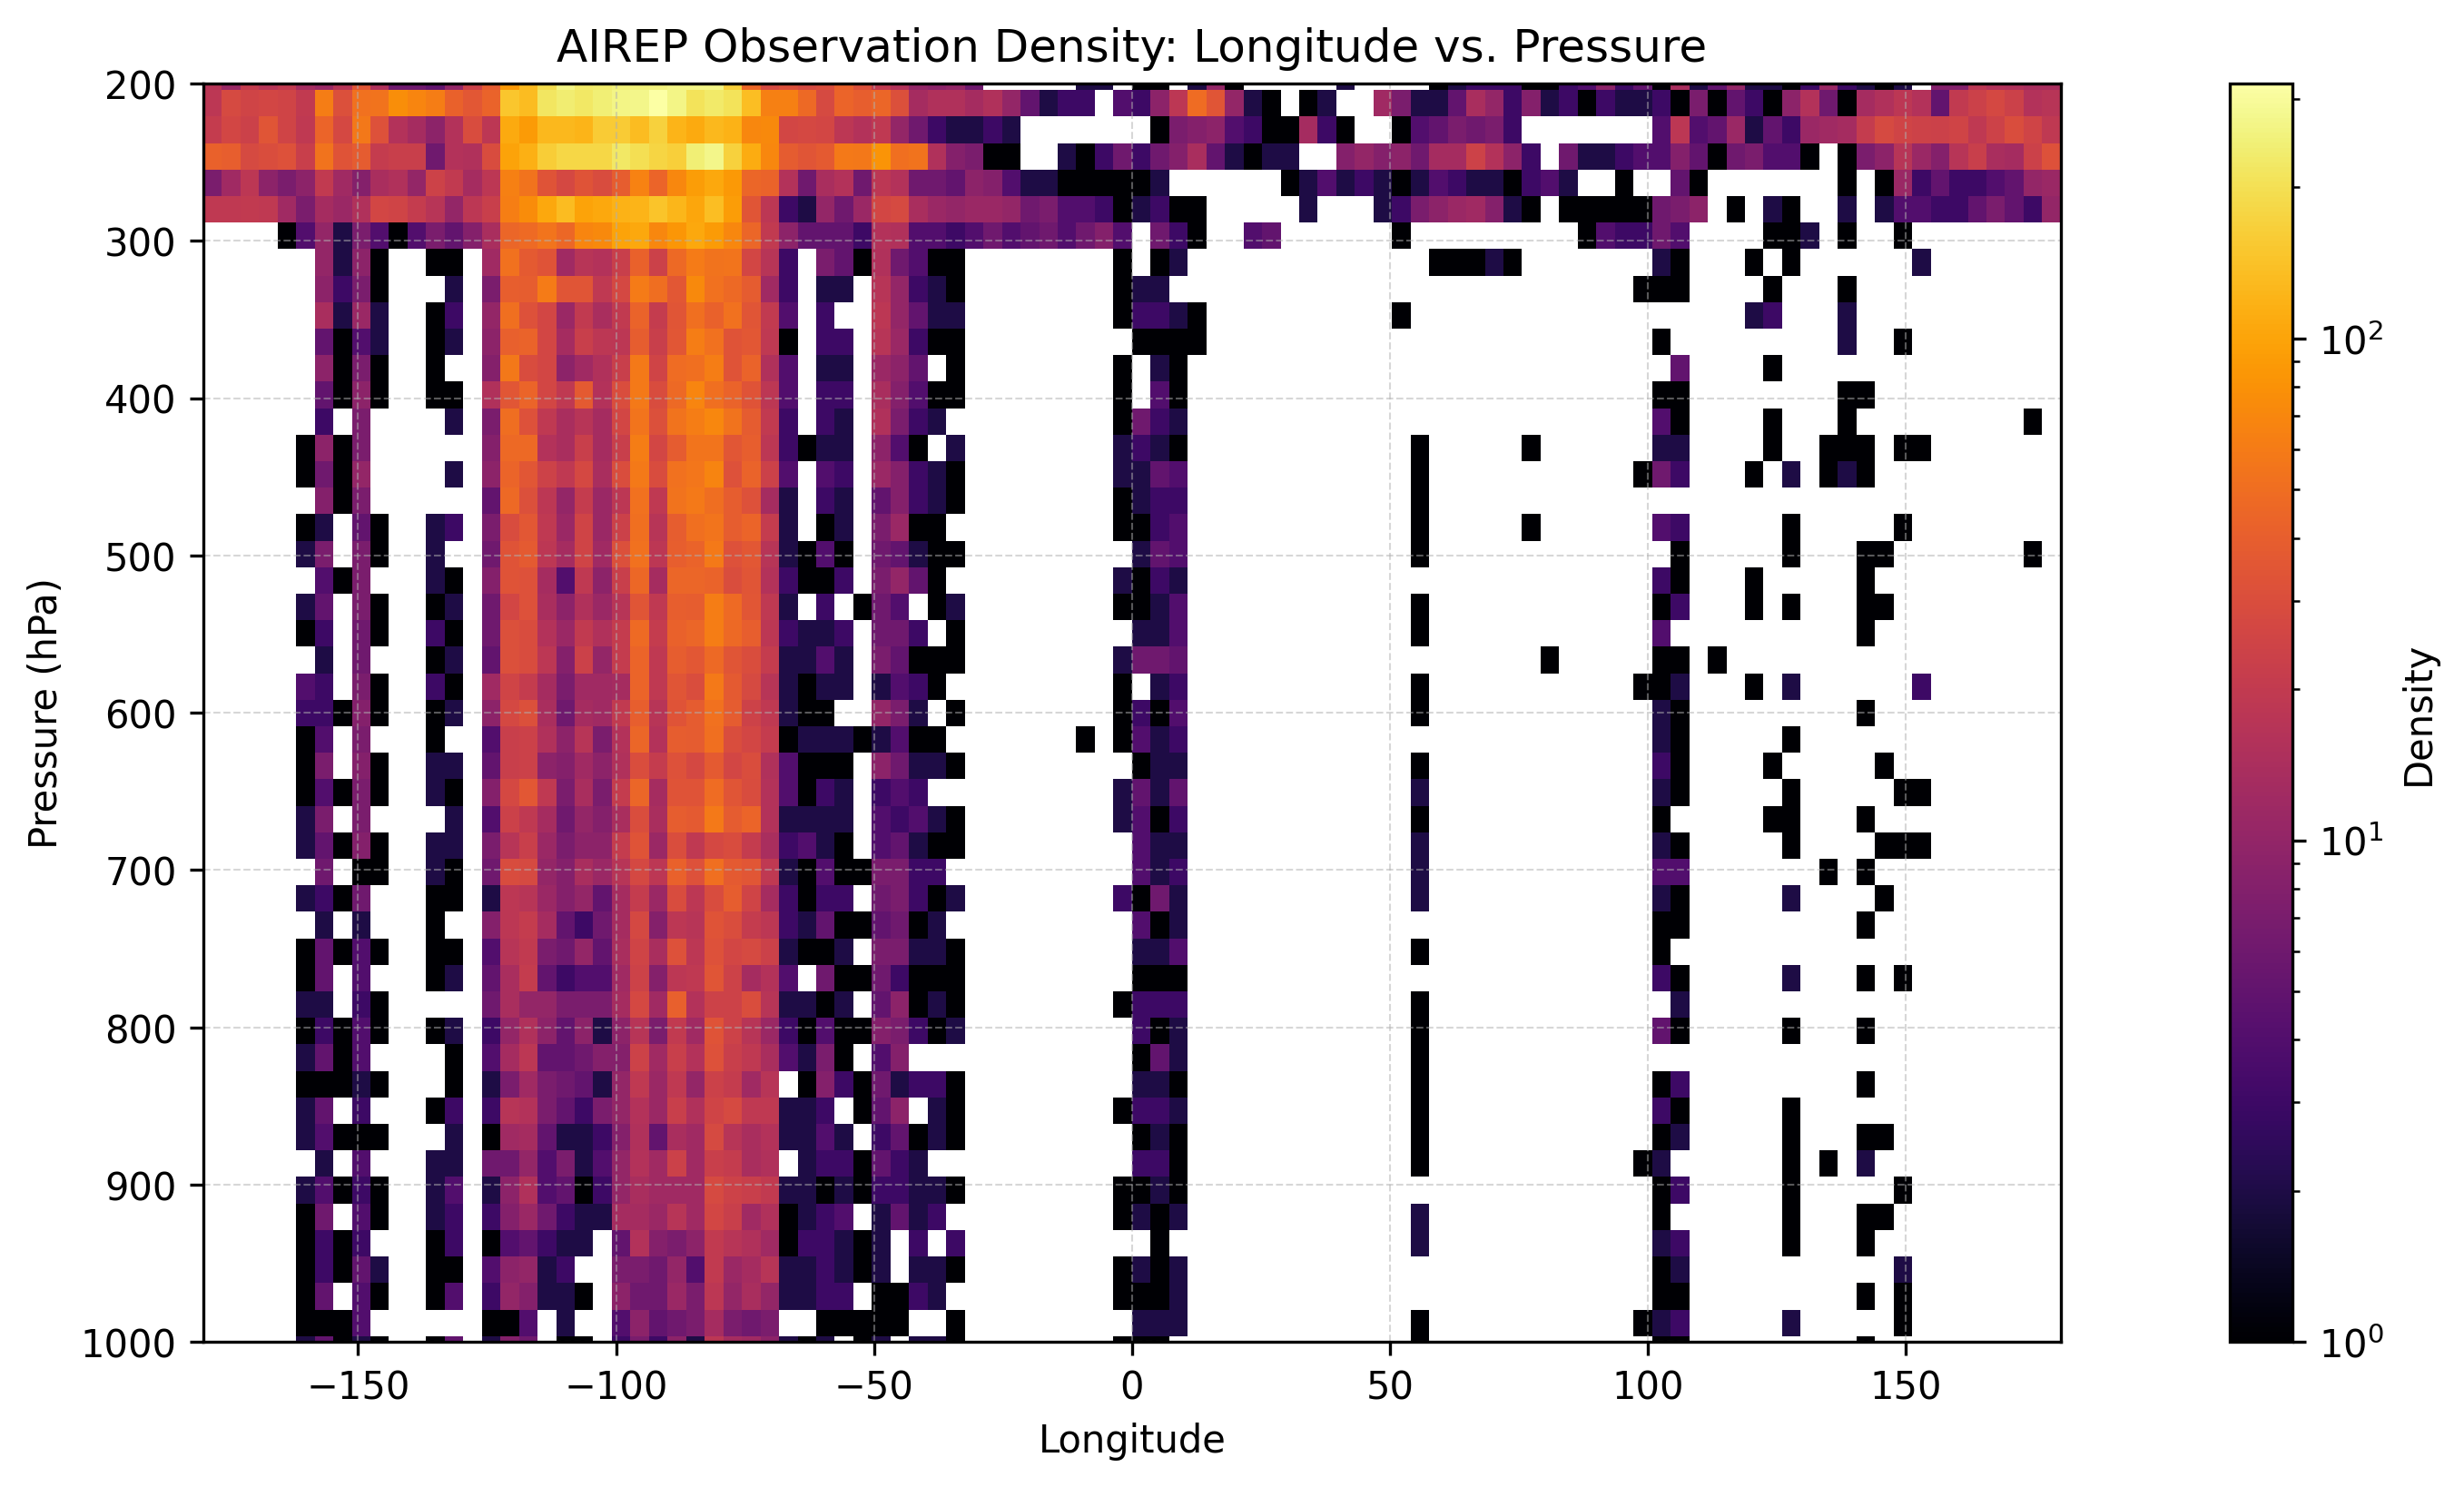
\includegraphics[width=0.9\textwidth]{images/airep_height_density.png}
    \caption{AIREP density vs vertical height in hPa and longitude.}
    \label{fig:airep_plot}
\end{figure}

The following code will generate a density distribution over height and longitudes. 

\begin{codeonly}{Vertical Distribution of AIRPE Observations}
def plot_height_histogram(lons, heights,
                           filename="airep_height_density.png"):
    """Generates a histogram of longitude vs. height, converting pressure
    to altitude with 1000 hPa at the bottom and 200 hPa at the top."""
    fig, ax = plt.subplots(figsize=(10, 6))
    
    # Convert pressure Pa to hPa 
    heights = heights / 100 
    
    # Create 2D histogram
    hist, xedges, yedges = np.histogram2d(lons, heights,
                                          bins=(100, 50))
    
    # Use the same optimized colormap as in global density plot
    pcm = ax.pcolormesh(xedges, yedges, hist.T, cmap='inferno',
                        norm=plt.matplotlib.colors.LogNorm(
                            vmin=hist[hist > 0].min(),
                            vmax=hist.max()))
    
    cbar = fig.colorbar(pcm, ax=ax, orientation='vertical',
                        fraction=0.04, pad=0.08)
    cbar.set_label("Density")
    
    plt.xlabel("Longitude")
    plt.ylabel("Pressure (hPa)")
    plt.title("AIREP Observation Density: Longitude vs. Pressure")
    plt.ylim(1000, 200)  # Invert y-axis so 1000 hPa is at bottom
    plt.grid(True, linestyle='--', linewidth=0.5, alpha=0.5)
    
    plt.savefig(filename, dpi=300, bbox_inches="tight")
    plt.show()
\end{codeonly}


\subsection{Plotting Scalar Fields on ICON Triangular Grids}

To visualize ICON model output fields on the native triangular grid, we combine the triangular mesh geometry from the ICON grid file with field values from the forecast GRIB file. This allows for accurate visualization of quantities such as temperature or land-sea mask using the \texttt{matplotlib} and \texttt{cartopy} libraries.

We demonstrate the full process below using the land-sea mask field \texttt{lsm} as an example.

\subsubsection*{Reading the ICON Grid}

The ICON grid file contains the geographical coordinates of each triangle vertex (\texttt{vlon}, \texttt{vlat}) and the connectivity table (\texttt{vertex\_of\_cell}) defining which three vertices form each triangle.

\begin{codeonly}{Reading the ICON Grid File}
import numpy as np
import matplotlib.tri as mtri
import netCDF4 as nc

gridfile = "icon_grid_0043_R02B04_G.nc"
print('Reading grid file:', gridfile)

with nc.Dataset(gridfile) as f:
    vlon = f['vlon'][:] * 180 / np.pi
    vlat = f['vlat'][:] * 180 / np.pi
    vertex_of_cell = f['vertex_of_cell'][:] - 1  # convert from 1-based to 0-based indexing

    triangulation = mtri.Triangulation(vlon, vlat, vertex_of_cell.T)
\end{codeonly}

\subsubsection*{Extracting Forecast Data from the GRIB File}

Forecast fields are read from a GRIB file using the \texttt{eccodes} interface. We use a helper function to extract the field matching a given short name:

\begin{codeonly}{Extracting Field from GRIB}
import eccodes

def extract_values(grib_file, sname):
    with open(grib_file, 'rb') as f:
        while True:
            gid = eccodes.codes_grib_new_from_file(f)
            if gid is None:
                break

            short_name = eccodes.codes_get(gid, "shortName")
            if short_name == sname:
                values = eccodes.codes_get_array(gid, "values")
                eccodes.codes_release(gid)
                return values

            eccodes.codes_release(gid)

    raise ValueError(f"shortName '{sname}' not found in {grib_file}")
\end{codeonly}

\begin{codeonly}{Reading the Field Data}
valfile = "fc_R02B04.2022010100"
values = extract_values(valfile, "lsm")  # land-sea mask
\end{codeonly}

\subsubsection*{Plotting the Field with Cartopy}

We use \texttt{cartopy} to overlay the triangulated scalar field on a map. The values are visualized using \texttt{tripcolor}, with a colorbar for interpretation.

\begin{codeonly}{Plotting the ICON Triangular Field}
import matplotlib.pyplot as plt
import cartopy.crs as ccrs

fig, ax = plt.subplots(figsize=(10, 5), subplot_kw={'projection': ccrs.PlateCarree()})

# Plot the scalar field on the triangulated grid
tpc = ax.tripcolor(triangulation, facecolors=values, cmap='viridis', shading='flat')

# Add map features
ax.coastlines()
ax.set_title("ICON Land-Sea Mask (triangular grid)")
plt.colorbar(tpc, ax=ax, shrink=0.8, label="Land-Sea Mask")

plt.savefig("images/icon_lsm_plot.png")
plt.show()
\end{codeonly}

\begin{center}
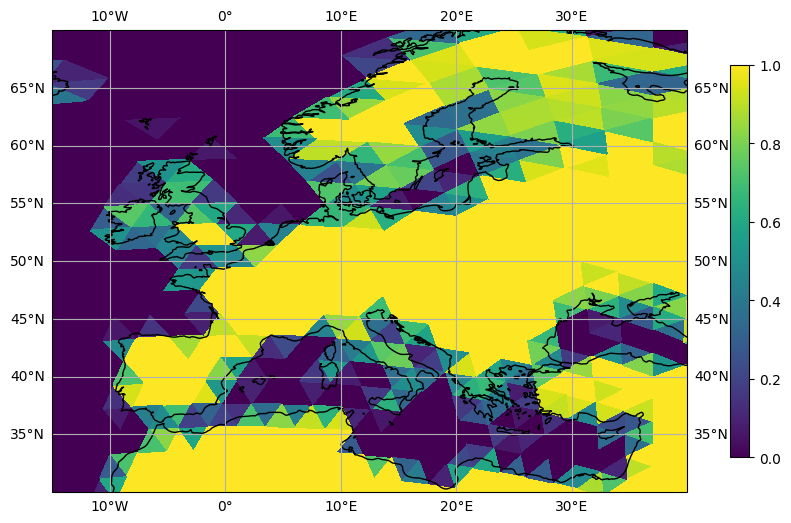
\includegraphics[width=0.9\textwidth]{images/icon_lsm_plot.png}
\end{center}

This method can be applied to any scalar field available in the forecast file, such as surface temperature (\texttt{T\_G}) or wind speed components (\texttt{10u}, \texttt{10v}). The same triangulation can be reused for all variables defined per triangle. The scripts will also work if fields are defined on triangle vertices, tripcolor is quite powerful.


 % eccodes, netcdf, fields and maps

\addtocontents{toc}{\noindent\hrulefill\vspace{-1.5ex}\par}
\addcontentsline{toc}{chapter}{\textcolor{dwdspecial}{\large Day 2: AI/ML Basic Introduction}}

\chapter{Basics of Artificial Intelligence and Machine Learning (AI/ML)}

%==============================================================================
%
%==============================================================================
\section{AI and ML - Basic Ideas}

Artificial Intelligence (AI) and Machine Learning (ML) are transforming the way problems are approached across various fields, including geosciences, weather forecasting, climate science, language processing, and decision-making. This section introduces AI and ML from three fundamental perspectives: as a problem-solving approach, as a set of tools, and as a new paradigm for interactivity and services.

\subsection{AI and ML as a Problem-Solving Approach}

Traditional problem-solving methods rely on explicit mathematical models based on domain knowledge. These models work well for structured problems but struggle with complex, high-dimensional data. AI and ML take a different approach:

\begin{itemize}
    \item \textbf{Data-Driven Learning}: Instead of defining rules explicitly, ML algorithms learn patterns from large datasets.
    \item \textbf{Universal Approximators}: Neural networks and other ML techniques act as function approximators, capable of modeling intricate relationships in data.
    \item \textbf{Applications Across Domains}: ML is revolutionizing fields such as weather forecasting, climate modeling, speech recognition, and autonomous systems.
\end{itemize}

One of the key concepts in ML is the approximation of an unknown function \( f(x) \) using a trained model \( \hat{f}(x) \). A neural network, for instance, seeks to minimize the error between the predicted and actual values:

\begin{equation}
    \min_{\theta} \sum_{i=1}^{N} L\big(y_i, \hat{f}(x_i; \theta)\big),
\end{equation}

where \( \theta \) represents the model parameters, \( x_i \) are input features, and \( y_i \) are the corresponding target values.

Though AI/ML tools are usually universally applicable, still their reliable application and deployment needs all the domain knowledge which is traditionally acquired and necessary for classical modelling and its application. AI/ML does not replace domain knowledge, but is an additional tool and technique to make domain scientists do their work in a better way. 

\subsection{AI and ML as a Set of Tools}

AI/ML development is supported by a growing ecosystem of frameworks, computational resources, and cloud-based services that make it more accessible than ever.

\textbf{Core Machine Learning Frameworks.} Several powerful frameworks provide the foundation for AI development:
\begin{itemize}
    \item \textbf{PyTorch} and \textbf{TensorFlow}: Widely used deep learning libraries that allow researchers and engineers to build, train, and deploy neural networks efficiently.
    \item \textbf{scikit-learn}: A robust library for traditional machine learning algorithms such as regression, clustering, and decision trees.
\end{itemize}

\textbf{AI as a Service.} Many pre-trained AI models and APIs allow users to integrate ML functionalities without requiring deep expertise in AI model building:
\begin{itemize}
    \item \textbf{LLMs as a Service}: Companies such as OpenAI, Google, and Meta provide access to state-of-the-art large language models via APIs.
    \item \textbf{On-Premise AI}: Locally installed models like Llama, Mistral, and DeepSeek enable AI applications without relying on cloud services and without the dependence on big tech companies.
\end{itemize}

\textbf{Computational Resources.} The performance of AI models depends heavily on the hardware and infrastructure used for training and inference:
\begin{itemize}
    \item \textbf{Local GPUs and TPUs}: Accelerate AI computations on personal or institutional hardware.
    \item \textbf{Cloud-Based AI Computing}: Platforms such as AWS, Google Cloud, and Azure provide scalable computing resources.
    \item \textbf{Edge Computing}: Optimized AI models can run on mobile devices and embedded systems, reducing reliance on centralized servers.
\end{itemize}

\subsection{AI and ML as a New Paradigm for Interactivity and Services}

Beyond being just tools, AI and ML are reshaping how humans interact with technology and how productivity can be enhanced across various industries. However, this transformation is not without its challenges. Many AI applications promise significant efficiency gains, but they also introduce risks such as reliability issues, ethical concerns, and the need for human oversight. Understanding these limitations is crucial to harness AI effectively.

\textbf{AI-Powered Productivity.} AI significantly improves efficiency and accelerates workflows:
\begin{itemize}
    \item \textbf{Code Assistants}: AI-powered tools, such as GitHub Copilot and ChatGPT-based interfaces, assist developers in writing, debugging, and optimizing code.
    \item \textbf{AI in Research}: AI facilitates the analysis of large datasets, aids in hypothesis generation, and automates repetitive tasks in scientific discovery.
\end{itemize}

\textbf{Critical Evaluation.} While AI-enhanced productivity is often presented as a game-changer, it also brings new dependencies and challenges. AI-generated code can contain errors that are difficult to detect, and over-reliance on AI in research may lead to superficial conclusions if users fail to critically assess AI-generated insights. Furthermore, the quality of AI output is only as good as the data it is trained on, making data curation and validation essential. Detecting errors in AI algorithms requires deep knowledge of both AI tools and the specific domain of application.

\textbf{AI in Decision Support.} AI is increasingly integrated into decision-making processes across multiple domains:
\begin{itemize}
    \item \textbf{Weather and Climate Services}: AI enhances forecasting models, improves risk assessment, and aids in climate trend analysis.
    \item \textbf{Healthcare}: AI supports medical diagnosis, enables personalized treatment recommendations, and assists in predictive analytics.
    \item \textbf{Autonomous Systems}: AI powers self-operating systems, including autonomous vehicles, robotics, and intelligent infrastructure.
\end{itemize}

\textbf{Critical Evaluation.} While AI has great potential in decision support, it also raises concerns about transparency, bias, and accountability. AI-driven forecasts and medical diagnostics must be interpretable and explainable to ensure trust. In high-stakes environments, blind reliance on AI can lead to severe consequences, making human oversight and hybrid AI-human decision-making crucial.

\textbf{The Need for AI Education.} As AI adoption grows, so does the necessity for education and training. For domain scientists, this means moving beyond traditional methods and integrating AI-driven approaches into their workflows.

\begin{itemize}
    \item Mastering AI frameworks enables domain experts to develop and refine tailored solutions.
    \item Understanding AI-powered services is crucial for their effective and responsible integration.
    \item Awareness of AI ethics and limitations is essential to ensure transparency, fairness, and accountability.
\end{itemize}

\textbf{Critical Evaluation.} The growing need for AI education is evident, but it also presents significant challenges. Many domain experts lack formal training in AI, making interdisciplinary collaboration essential. Additionally, AI education must go beyond technical aspects to include discussions on ethical AI use, bias mitigation, and responsible development. Without a strong foundation in these areas, AI could be misused or misinterpreted, leading to unreliable results. 

Many AI experts approach domain problems with the assumption that data-driven models can replace traditional expertise, often underestimating the complexity and contextual knowledge required for accurate interpretation. This overconfidence can lead to models that appear to perform well on benchmarks but fail in real-world applications due to overlooked domain-specific constraints and hidden biases.

\subsection{Conclusion}

AI and ML are more than just tools—they represent a fundamental shift in problem-solving, technology, and human-computer interaction. From universal approximators to AI-driven interactive services, these methods continue to reshape industries and scientific research. As AI adoption grows, so does the need for structured education and expertise in this rapidly evolving field.

\begin{recommendationbox}
The tools available today by AI/ML technology are representing a technological shift. Develop a balanced view, which sees the potential and the limitations at the same time. The shift can be compared to the development of book copying technology, radio or the invention of flight. 
\end{recommendationbox}

%==============================================================================
%
%==============================================================================
\section{\texttt{Torch Tensors} - Basics and Their Role in Minimization}

Deep learning frameworks simplify the development and deployment of machine learning models, but they must balance flexibility, efficiency, and ease of use. PyTorch has emerged as one of the most widely adopted frameworks because it combines an intuitive, Pythonic interface with powerful automatic differentiation and dynamic computation graph capabilities. Unlike static graph-based frameworks, PyTorch allows for more flexible model development, making it particularly useful for research, experimentation, and rapid prototyping. Its seamless GPU acceleration, built-in support for deep learning libraries, and strong community adoption make it a critical tool for both academic and industrial AI applications.


Torch tensors are the fundamental data structures in PyTorch. They are similar to NumPy arrays but come with additional capabilities, such as GPU acceleration and automatic differentiation, which are essential for training neural networks. In particular, tensors with the attribute \texttt{requires\_grad=True} allow PyTorch to automatically compute gradients, a key component in optimization algorithms like gradient descent.

Below, we illustrate basic tensor operations and demonstrate how tensors enable minimization through gradient computation.

\begin{codeonly}{Tensor Operations and Gradients}
import torch

# Create a tensor from a Python list
a = torch.tensor([1.0, 2.0, 3.0])
print("Tensor a:", a)

# Create a 3x3 tensor with random values
b = torch.rand(3, 3)
print("Random tensor b:\n", b)

# Perform arithmetic: multiply tensor 'a' by 2
c = a * 2
print("Tensor c (a multiplied by 2):", c)

# For minimization, we need tensors that track gradients.
# Create a tensor with requires_grad=True so that operations on it are tracked.
x = torch.tensor([2.0, 3.0], requires_grad=True)

# Define a simple quadratic function: f(x) = x[0]^2 + x[1]^2
y = x[0]**2 + x[1]**2

# Compute gradients with respect to x using backpropagation
y.backward()

# The gradients of y with respect to x are stored in x.grad
print("Gradients of y with respect to x:", x.grad)
\end{codeonly}

%start_codeframe
%\includeexternalcode{code-ch04-sec01-tensor-operations-and-gradients}{code-ch04-sec01-tensor-operations-and-gradients.py}  % Original includeexternalcode
%start_code_output

\textbf{Output:}
\begin{lstlisting}
Tensor a: tensor([1., 2., 3.])
Random tensor b:
 tensor([[0.3450, 0.2811, 0.0059],
        [0.6343, 0.5166, 0.4793],
        [0.3613, 0.5797, 0.5450]])
Tensor c (a multiplied by 2): tensor([2., 4., 6.])
Gradients of y with respect to x: tensor([4., 6.])
\end{lstlisting}

%\lstinputlisting{code/code-ch04-sec01-tensor-operations-and-gradients.txt}
%end_codeframe

In this example, we compute the gradient of a quadratic function, which is a common operation in optimization tasks. When training a neural network, the loss function is minimized by iteratively updating the model parameters (stored as tensors) based on their computed gradients. This automatic differentiation capability is crucial for efficient and effective model training.

\begin{recommendationbox}
Automatic gradient calculation, optimization, and learning are at the core of the technological transformation.
\end{recommendationbox}

%==============================================================================
%
%==============================================================================
\section{\texttt{PyTorch Fundamentals} - Model, Loss, and Optimizer}

First, let us install the necessary packages in our Python virtual environment. This step is assumed to be done already, we discussed how to install python packages in various environments in depth in the preceding parts of this tutorial. 

Now, in your Python program, either directly in a .py file or a Jupyter Notebook, you need to import the required packages.

\begin{codeonly}{Torch Packages}
import torch
import torch.nn as nn
import torch.optim as optim
\end{codeonly}

%start_codeframe
%\includeexternalcode{code-ch04-sec02-torch-nn-optim}{code-ch04-sec02-torch-nn-optim.py}  % Original includeexternalcode
%start_code_output
%end_codeframe

Next, we define a dataset to train on. In many of our examples we create synthetic data. For instance, you may generate random data for regression or classification tasks, or, as in the sine curve example below, data derived from mathematical functions. Often, the dataset is split into training and testing subsets to evaluate model performance and to prevent overfitting.

Below is an example code that sets up training and test data for a generic regression task. Here, we generate random input features and corresponding target values:

\begin{codeonly}{Synthetic Data}
import torch
import numpy as np
from torch.utils.data import TensorDataset, DataLoader

# Generate synthetic data: 100 samples with 10 features each
X = np.random.rand(100, 10)
y = np.random.rand(100, 1)

# Convert numpy arrays to torch tensors
X_tensor = torch.tensor(X, dtype=torch.float32)
y_tensor = torch.tensor(y, dtype=torch.float32)

# Create a TensorDataset and then split it into training and test sets
dataset = TensorDataset(X_tensor, y_tensor)
train_size = int(0.8 * len(dataset))
test_size = len(dataset) - train_size
train_dataset, test_dataset = torch.utils.data.random_split(dataset, [train_size, test_size])

# Diagnostic Output
print(f"Train dataset size: {len(train_dataset)}, Test dataset size: {len(test_dataset)}")

# Show shapes of the first batch
first_train_sample = train_dataset[0]
print(f"First training sample - X shape: {first_train_sample[0].shape}, y shape: {first_train_sample[1].shape}")

# Show content of the first training sample
print(f"First training sample - X: {first_train_sample[0].numpy()}, y: {first_train_sample[1].numpy()}")
\end{codeonly}

%start_codeframe
%\includeexternalcode{code-ch04-sec02-generate-synthetic-data-split}{code-ch04-sec02-generate-synthetic-data-split.py}  % Original includeexternalcode
%start_code_output

\textbf{Output:}
\begin{lstlisting}
Train dataset size: 80, Test dataset size: 20
First training sample - X shape: torch.Size([10]), y shape: torch.Size([1])
First training sample - X: [0.2555835  0.13075094 0.1967931  0.3170668  0.08261041 0.68258333
 0.92773515 0.7652774  0.07989042 0.28203908], y: [0.06629485]
\end{lstlisting}

%\lstinputlisting{code/code-ch04-sec02-generate-synthetic-data-split.txt}
%end_codeframe


Now, let us define a simple neural network with one hidden layer. This network consists of an input layer, one hidden layer with a ReLU activation, and an output layer.

\begin{codeonly}{Simple NN Model}
import torch
import torch.nn as nn
import torch.optim as optim

class SimpleNN(nn.Module):
    def __init__(self, input_size, hidden_size, output_size):
        super(SimpleNN, self).__init__()
        self.fc1 = nn.Linear(input_size, hidden_size)
        self.relu = nn.ReLU()
        self.fc2 = nn.Linear(hidden_size, output_size)
        
    def forward(self, x):
        x = self.fc1(x)
        x = self.relu(x)
        x = self.fc2(x)
        return x

# Instantiate the model
input_size = 10
hidden_size = 16
output_size = 1
model = SimpleNN(input_size, hidden_size, output_size)

# Define the loss function and optimizer
criterion = nn.MSELoss()
optimizer = torch.optim.Adam(model.parameters(), lr=0.01)

print(model)
\end{codeonly}

%start_codeframe
%\includeexternalcode{code-ch04-sec02-simple-nn-model}{code-ch04-sec02-simple-nn-model.py}  % Original includeexternalcode
%start_code_output

\textbf{Output:}
\begin{lstlisting}
SimpleNN(
  (fc1): Linear(in_features=10, out_features=16, bias=True)
  (relu): ReLU()
  (fc2): Linear(in_features=16, out_features=1, bias=True)
)
\end{lstlisting}

%\lstinputlisting{code/code-ch04-sec02-simple-nn-model.txt}
%end_codeframe

The script begins by importing the necessary PyTorch modules: \texttt{torch} for core functionalities, \texttt{torch.nn} for neural network components, and \texttt{torch.optim} for optimization algorithms.

A simple feedforward neural network is defined using the \texttt{SimpleNN} class, which inherits from \texttt{nn.Module}. The network consists of two fully connected layers. The first layer (\texttt{fc1}) maps the input features to a hidden layer, followed by a ReLU activation function to introduce non-linearity. The second layer (\texttt{fc2}) maps the hidden layer to the output layer. The forward pass is computed as:
\begin{equation}
    x = \text{fc1}(x) \rightarrow \text{ReLU}(x) \rightarrow \text{fc2}(x).
\end{equation}

The model is instantiated with three parameters: \texttt{input\_size = 10}, representing the number of input features, \texttt{hidden\_size = 16}, defining the number of neurons in the hidden layer, and \texttt{output\_size = 1}, indicating a single output value, which is appropriate for regression tasks.

To train the model, the loss function is set to Mean Squared Error (MSE), given by:
\begin{equation}
    \mathcal{L} = \frac{1}{N} \sum_{i=1}^{N} (y_i - \hat{y}_i)^2.
\end{equation}
The Adam optimizer is used to update the model parameters with a learning rate of 0.01.

Finally, the model architecture is printed to verify its structure.

{\bf The Adam Optimizer.}
The Adam optimizer (Adaptive Moment Estimation) uses the first moment estimate $\mathbf{m_t}$ and the second moment estimate $\mathbf{v_t}$ to compute an adaptive learning rate for each parameter.

1. {\em First moment estimate} $\mathbf{m_t}$: This is an exponentially weighted moving average of past gradients, representing a smoothed estimate of the mean gradient:
   \begin{equation}
       m_t = \beta_1 m_{t-1} + (1 - \beta_1) g_t.
   \end{equation}
   Since $\mathbf{m_t}$ starts from zero, Adam applies bias correction:
   \begin{equation}
       \hat{m}_t = \frac{m_t}{1 - \beta_1^t}.
   \end{equation}
   This correction ensures that $\hat{m}_t$ is an unbiased estimate of the true gradient expectation.

2. {\em Second moment estimate} $\mathbf{v_t}$: This is an exponentially weighted moving average of past squared gradients, approximating the variance of the gradient:
   \begin{equation}
       v_t = \beta_2 v_{t-1} + (1 - \beta_2) g_t^2.
   \end{equation}
   Similar to $\mathbf{m_t}$, Adam applies bias correction:
   \begin{equation}
       \hat{v}_t = \frac{v_t}{1 - \beta_2^t}.
   \end{equation}
   This correction ensures that $\hat{v}_t$ is an unbiased estimate of the second moment.

3. {\em Parameter update}: Using the corrected estimates $\mathbf{\hat{m}_t}$ and $\mathbf{\hat{v}_t}$, Adam updates the parameters $\mathbf{\theta}$ as follows:
   \begin{equation}
       \theta_{t+1} = \theta_t - \frac{\eta}{\sqrt{\hat{v}_t} + \epsilon} \hat{m}_t.
   \end{equation}
   Here, $\mathbf{\eta}$ is the learning rate, and $\mathbf{\epsilon}$ is a small constant to prevent division by zero.

In summary, Adam normalizes the gradient update using the estimated first and second moments, allowing each parameter to have an individual learning rate that adapts to the scale of its gradients. This leads to more stable and efficient optimization compared to standard gradient descent.



%==============================================================================
%
%==============================================================================
\subsection{\texttt{Data Handling} - Dataset and DataLoader}

Neural networks are typically trained on large datasets, making it inefficient to load all data into memory at once. Instead, \textbf{data loaders} are used to efficiently handle batch processing, shuffling, and parallel loading.

Given a dataset with input samples $\mathbf{X} = \{x_1, x_2, \dots, x_N\}$ and corresponding labels $\mathbf{Y} = \{y_1, y_2, \dots, y_N\}$, a data loader divides the dataset into mini-batches of size $B$. At each training step, the model processes a batch:
\begin{equation}
    (\mathbf{X}_B, \mathbf{Y}_B) = \{(x_i, y_i)\}_{i=1}^{B}.
\end{equation}

Key advantages of using data loaders include:
\begin{itemize}
    \item \textbf{Memory efficiency}: Only small batches are loaded into memory at a time.
    \item \textbf{Shuffling}: Randomizing data order prevents overfitting to specific patterns.
    \item \textbf{Parallel processing}: Multiple CPU threads can load data asynchronously.
\end{itemize}

In PyTorch, a \texttt{DataLoader} automates these tasks, enabling efficient training on large datasets.

After installing the necessary packages, you can use PyTorch's DataLoader to efficiently handle data in mini-batches. This is particularly useful for training, as it enables you to iterate over the dataset in smaller chunks, reducing memory usage and often improving convergence. Here's an example using synthetic data with a TensorDataset.

We use the tensors \texttt{X\_tensor} and \texttt{y\_tensor} from above. 

\begin{codeonly}{Data Loader}
from torch.utils.data import DataLoader

# Create a DataLoader for the training dataset
dataloader = DataLoader(train_dataset, batch_size=16, shuffle=True)

# Example: Iterate through one batch
n = 1
for batch_X, batch_y in dataloader:
    print(f"{n}) Batch X shape:", batch_X.size())
    print("      Batch y shape:", batch_y.size())
    n += 1
\end{codeonly}

%start_codeframe
%\includeexternalcode{code-ch04-sec02-data-loader-batch-example}{code-ch04-sec02-data-loader-batch-example.py}  % Original includeexternalcode
%start_code_output

\textbf{Output:}
\begin{lstlisting}
1) Batch X shape: torch.Size([16, 10])
      Batch y shape: torch.Size([16, 1])
2) Batch X shape: torch.Size([16, 10])
      Batch y shape: torch.Size([16, 1])
3) Batch X shape: torch.Size([16, 10])
      Batch y shape: torch.Size([16, 1])
4) Batch X shape: torch.Size([16, 10])
      Batch y shape: torch.Size([16, 1])
5) Batch X shape: torch.Size([16, 10])
      Batch y shape: torch.Size([16, 1])
Selection deleted
\end{lstlisting}
%\lstinputlisting{code/code-ch04-sec02-data-loader-batch-example.txt}

%end_codeframe

In the example from above, the dataset contains $N = 100$ samples, which is split into:
\begin{itemize}
    \item \textbf{Training set:} 80 samples
    \item \textbf{Test set:} 20 samples
\end{itemize}
The script creates a \texttt{DataLoader} that loads batches of data from the training dataset. Each batch consists of 16 samples, with:
\begin{itemize}
    \item \textbf{Batch X shape}: $(16,10)$, meaning each batch contains 16 feature vectors, each with 10 features.
    \item \textbf{Batch y shape}: $(16,1)$, meaning each batch contains 16 target values, each a scalar.
\end{itemize}

\begin{enumerate}
    \item The loop runs exactly 5 times because the dataset contains 80 training samples, and the batch size is 16. 
    \item Each iteration produces a batch of size 16, confirming that the \texttt{DataLoader} correctly partitions the dataset.
    \item Since \texttt{shuffle=True}, the data order is randomized, ensuring that each epoch has a different sample arrangement.
\end{enumerate}

The \texttt{DataLoader} successfully partitions the dataset into evenly sized mini-batches, verifying that the batch processing mechanism functions as expected.

%==============================================================================
%
%==============================================================================
\section{Simple Neural Network Training Example}

We now develop an example that demonstrates how to approximate the sine function using a simple neural network built with PyTorch. We generate data from the sine curve, create a dataset with a DataLoader for mini-batch training, define a neural network model, train it using mean squared error loss, and finally plot the network's predictions against the actual sine values.

\begin{codeonly}{Sine Curve Approximation}
import torch
import torch.nn as nn
import torch.optim as optim
import numpy as np
import matplotlib.pyplot as plt
from torch.utils.data import TensorDataset, DataLoader

# Generate dataset for sine curve approximation
x = np.linspace(0, 2 * np.pi, 1000)
y = np.sin(x)

# Convert numpy arrays to torch tensors and add a feature dimension
x_tensor = torch.tensor(x, dtype=torch.float32).unsqueeze(1)
y_tensor = torch.tensor(y, dtype=torch.float32).unsqueeze(1)

# Create a TensorDataset and DataLoader for batch processing
dataset = TensorDataset(x_tensor, y_tensor)
dataloader = DataLoader(dataset, batch_size=32, shuffle=True)

# Define a simple neural network model
class SineModel(nn.Module):
    def __init__(self):
        super(SineModel, self).__init__()
        self.net = nn.Sequential(
            nn.Linear(1, 16),
            nn.ReLU(),
            nn.Linear(16, 16),
            nn.ReLU(),
            nn.Linear(16, 1)
        )
    
    def forward(self, x):
        return self.net(x)

model = SineModel()

# Set up the loss function and optimizer
criterion = nn.MSELoss()
optimizer = torch.optim.Adam(model.parameters(), lr=0.01)

# Training loop
num_epochs = 500
for epoch in range(num_epochs):
    for batch_x, batch_y in dataloader:
        optimizer.zero_grad()
        outputs = model(batch_x)
        loss = criterion(outputs, batch_y)
        loss.backward()
        optimizer.step()
    if (epoch + 1) % 100 == 0:
        print(f'Epoch [{epoch+1}/{num_epochs}], Loss: {loss.item():.4f}')

# Generate predictions after training
with torch.no_grad():
    predicted = model(x_tensor).detach().numpy()

# Plot the actual sine curve and the network's predictions
plt.figure(figsize=(8, 4))
plt.plot(x, y, label='Actual Sine')
plt.plot(x, predicted, label='Predicted Sine', linestyle='--')
plt.xlabel('x')
plt.ylabel('sin(x)')
plt.legend()
plt.savefig("sine_approximation.png")
\end{codeonly}
%start_codeframe
%\includeexternalcode{code-ch04-sec03-sine-curve-approximation}{code-ch04-sec03-sine-curve-approximation.py}  % Original includeexternalcode
%start_code_output

\textbf{Output:}
\begin{lstlisting}
Epoch [100/500], Loss: 0.0007
Epoch [200/500], Loss: 0.0005
Epoch [300/500], Loss: 0.0002
Epoch [400/500], Loss: 0.0003
Epoch [500/500], Loss: 0.0002
\end{lstlisting}
%\lstinputlisting{code/code-ch04-sec03-sine-curve-approximation.txt}

\textbf{Generated Image:}
\begin{figure}[ht] \centering
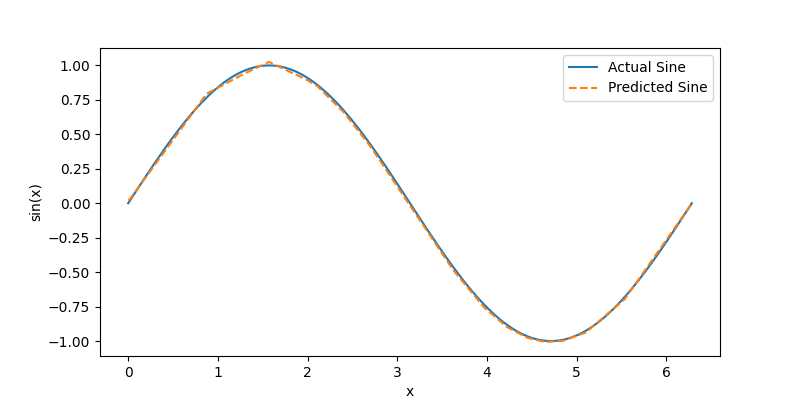
\includegraphics[width=0.8\textwidth]{images/code-ch04-sec03-sine_approximation.png}
\end{figure}
%end_codeframe

This code implements a neural network in PyTorch to approximate the sine function using supervised learning.

\textbf{Dataset Generation:}  
The input values are generated using:
\begin{equation}
    x = \text{linspace}(0, 2\pi, 1000).
\end{equation}
The target values are computed as:
\begin{equation}
    y = \sin(x).
\end{equation}
The NumPy arrays are converted into PyTorch tensors, with an additional feature dimension added using \texttt{unsqueeze(1)}.

\textbf{DataLoader for Batch Processing:}  
A \texttt{TensorDataset} is created, containing the input-output pairs $(x, y)$, and a \texttt{DataLoader} is used with a batch size of 32 and shuffling enabled.

\textbf{Neural Network Model:}  
The model consists of a simple feedforward neural network with:
\begin{itemize}
    \item An input layer with 1 neuron.
    \item Two hidden layers with 16 neurons each, followed by ReLU activation.
    \item An output layer with 1 neuron.
\end{itemize}
Mathematically, the forward pass is:
\begin{equation}
    \hat{y} = W_3 (\max(0, W_2 (\max(0, W_1 x + b_1)) + b_2)) + b_3.
\end{equation}

\textbf{Loss Function and Optimizer:}  
The Mean Squared Error (MSE) loss function is used:
\begin{equation}
    \mathcal{L} = \frac{1}{N} \sum_{i=1}^{N} (y_i - \hat{y}_i)^2.
\end{equation}
The optimizer is Adam with a learning rate of 0.01.

\textbf{Training Process:}  
The model is trained for 500 epochs. In each epoch:
\begin{enumerate}
    \item Gradients are reset using \texttt{optimizer.zero\_grad()}.
    \item Predictions are computed with \texttt{model(batch\_x)}.
    \item The loss is calculated using \texttt{criterion(outputs, batch\_y)}.
    \item Backpropagation updates the weights via \texttt{loss.backward()} and \texttt{optimizer.step()}.
\end{enumerate}
A progress message is printed every 100 epochs.

\textbf{Prediction and Visualization:}  
After training, the model predicts values for the entire dataset, and the results are plotted:
\begin{itemize}
    \item The original sine function is plotted as a solid line.
    \item The neural network's predictions are plotted as a dashed line.
\end{itemize}
The resulting plot is saved as \texttt{sine\_approximation.png}.

Programming with tensors in PyTorch requires careful handling to ensure that the automatic differentiation mechanism remains intact. PyTorch’s computational graphs track tensor operations dynamically, allowing gradients to be computed automatically via backpropagation. 

If operations are performed outside the tensor framework—such as converting tensors to NumPy arrays and then performing computations—the graph structure is lost, and gradient tracking is broken! This disrupts the minimization process, making parameter updates impossible. 

To maintain gradient tracking, all computations within the model and loss function must be conducted using PyTorch tensor operations. Additionally, tensors should be created with \texttt{requires\_grad=True} when gradients are needed, and \texttt{detach()} should be used only when explicitly removing a tensor from the computational graph, such as for inference or visualization. 

Proper tensor management ensures that PyTorch can fully automate gradient computations, enabling efficient and correct optimization.

\begin{recommendationbox}
Use the sine approximation as generic example, what AI/ML approximators do. Nonlinear mappings are approximated. Scaling this to a huge space, very high-dimensional non-linear mappings like language generation or weather prediction are approximated. 
\end{recommendationbox}

%==============================================================================
%
%==============================================================================
\section{Gradient Field and Decision Boundary}

Neural networks provide flexible solutions to complex classification problems. Here, we construct an example where the decision boundary is \textbf{highly nonlinear}, making it challenging for traditional linear classifiers. 

We utilize PyTorch's automatic differentiation to analyze the \textbf{gradient field} of the classification function, revealing the sensitivity of the learned model in different regions.

{\bf Generating Data with Two Shifted Ellipses.} To illustrate this, we generate synthetic data where points belong to \textbf{one of two elliptical regions}, each with different orientations and positions.

\begin{codeonly}{Data for Classification}
# Set random seed for reproducibility
torch.manual_seed(42)
np.random.seed(42)

N = 900  # Number of samples

# Generate the same random points in the range [-2, 2] x [-2, 2]
X = torch.rand(N, 2) * 4 - 2  # Unchanged points

# Define parameters for two smaller, shifted ellipses
a1, b1 = 1.0, 0.5
a2, b2 = 0.6, 0.9
theta1 = np.radians(30)
theta2 = np.radians(-45)
center1 = torch.tensor([0.9, 0.9])
center2 = torch.tensor([-1.1, -0.2])

X_shifted1 = X - center1
X_shifted2 = X - center2

x1_rot = X_shifted1[:, 0] * np.cos(theta1) + X_shifted1[:, 1] * np.sin(theta1)
y1_rot = -X_shifted1[:, 0] * np.sin(theta1) + X_shifted1[:, 1] * np.cos(theta1)
inside_ellipse1 = ((x1_rot / a1) ** 2 + (y1_rot / b1) ** 2) < 1

x2_rot = X_shifted2[:, 0] * np.cos(theta2) + X_shifted2[:, 1] * np.sin(theta2)
y2_rot = -X_shifted2[:, 0] * np.sin(theta2) + X_shifted2[:, 1] * np.cos(theta2)
inside_ellipse2 = ((x2_rot / a2) ** 2 + (y2_rot / b2) ** 2) < 1

labels = (inside_ellipse1 | inside_ellipse2).float().unsqueeze(1).numpy()

plt.figure(figsize=(7, 5))
plt.scatter(X[:, 0], X[:, 1], c=labels.squeeze(), cmap="bwr", alpha=1, edgecolors="white")
plt.xlabel("Feature 1")
plt.ylabel("Feature 2")
plt.title("Labels Defined by Two Smaller, Shifted Ellipses")
plt.xlim(-2, 2)
plt.ylim(-2, 2)
plt.grid()
plt.colorbar()
plt.savefig("points_labled.png")
plt.show()
\end{codeonly}

This script:
\begin{itemize}
    \item Generates $N=900$ random points within the range $[-2,2] \times [-2,2]$.
    \item Assigns labels based on \textbf{two ellipses with different centers and rotations}.
    \item Uses the \textbf{blue-white-red (BWR) color map} to differentiate classes.
    \item Saves the figure for later comparison.
\end{itemize}

\begin{figure}
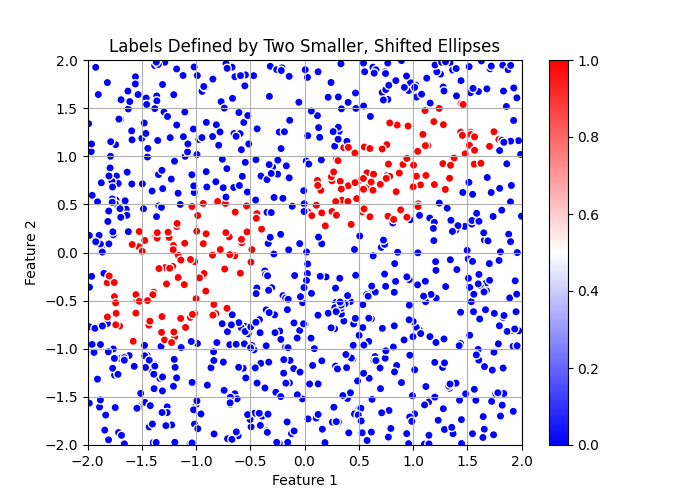
\includegraphics[width=0.5\textwidth]{images/points_labled.png}
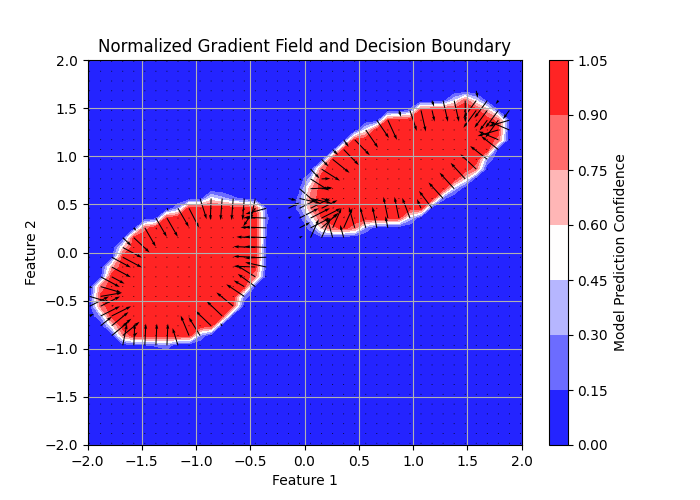
\includegraphics[width=0.5\textwidth]{images/points_classified_with_gradients.png}
\caption{The left figure shows the original data with class labels, while the right figure presents the classification result with \textbf{gradient information} extracted from the trained model.}
\end{figure}

{\bf Training a Neural Network for Classification.} We define a \textbf{simple feedforward neural network} with a single fully connected layer that maps the \textbf{two-dimensional input} to a binary classification output using the sigmoid activation function.

\begin{codeonly}{SimpleClassifier}
class BetterClassifier(nn.Module):
    def __init__(self):
        super().__init__()
        self.net = nn.Sequential(
            nn.Linear(2, 32),
            nn.ReLU(),
            nn.Linear(32, 1),
            nn.Sigmoid()
        )
    
    def forward(self, x):
        return self.net(x)

model = BetterClassifier()
\end{codeonly}

The model consists of:
\begin{itemize}
    \item A \textbf{fully connected layer} mapping two input features to a single output.
    \item A \textbf{sigmoid activation function} to produce probabilities.
\end{itemize}

Next, we train the model using the \textbf{binary cross-entropy loss function} and the \textbf{Adam optimizer}.

\begin{codeonly}{Classifier Training Loop}
import torch.optim as optim

criterion = nn.BCELoss()
optimizer = optim.Adam(model.parameters(), lr=0.01)

num_epochs = 1000
for epoch in range(num_epochs):
    optimizer.zero_grad()
    y_pred = model(X)
    loss = criterion(y_pred, torch.tensor(labels, dtype=torch.float32))
    loss.backward()
    optimizer.step()

    if (epoch + 1) % 200 == 0:
        print(f"Epoch {epoch+1}/{num_epochs}, Loss: {loss.item():.4f}")
\end{codeonly}

{\bf Decision Boundary and Gradient Visualization.} Once trained, the model is evaluated on a {\em dense grid of points} spanning the same input range $[-2,2] \times [-2,2]$. This allows us to {\em visualize the decision boundary} and analyze the {\em gradient} of the labels (classification) with respect to the features (input).

\begin{codeonly}{Display of Classification and Gradients}

x_min, x_max = X[:, 0].min() - 0.5, X[:, 0].max() + 0.5
y_min, y_max = X[:, 1].min() - 0.5, X[:, 1].max() + 0.5
xx, yy = torch.meshgrid(torch.linspace(x_min, x_max, 50),
                        torch.linspace(y_min, y_max, 50),
                        indexing='ij')

grid_points = torch.stack([xx.flatten(), yy.flatten()], dim=1)  
grid_points.requires_grad = True

grid_preds = model(grid_points)
grid_preds.backward(torch.ones_like(grid_preds))
grid_grads = grid_points.grad.detach().numpy()

grad_magnitudes = np.linalg.norm(grid_grads, axis=1, keepdims=True)
grad_magnitudes = np.clip(grad_magnitudes, 1, 1000)
grid_grads /= grad_magnitudes

grid_grads_x = grid_grads[:, 0].reshape(xx.shape)
grid_grads_y = grid_grads[:, 1].reshape(xx.shape)
grid_preds_np = grid_preds.detach().numpy().reshape(xx.shape)

plt.figure(figsize=(7, 5))
plt.contourf(xx, yy, grid_preds_np, alpha=1, cmap="bwr")
plt.colorbar(label="Model Prediction Confidence")
plt.quiver(xx, yy, grid_grads_x, grid_grads_y, color="black", scale=20)
plt.xlabel("Feature 1")
plt.ylabel("Feature 2")
plt.title("Normalized Gradient Field and Decision Boundary")
plt.xlim(-2, 2)
plt.ylim(-2, 2)
plt.grid()
plt.savefig("points_classified_with_gradients.png")
plt.show()
\end{codeonly}

This script computes model predictions over a uniform 50×50 grid, extracts gradients to analyze the sensitivity of the classifier, normalizes the gradients to limit their maximum size, uses contour plots to show the learned decision boundary, and overlays quiver arrows to indicate the gradient field.

\textbf{Observations.} The decision boundary adapts to the elliptical structures. The gradient arrows show where the model is most sensitive. Large gradients appear near the decision boundary, where small changes in input strongly impact classification.

The final visualization provides \textbf{deep insights into how the neural network classifies data}, demonstrating the potential of PyTorch's \textbf{autograd system} for analyzing decision boundaries.

\begin{recommendationbox}
AI/ML techniques provide a rather simple approach to solve a large variety of problems. How will physical arguments and further knowledge about the particular domain or problem under consideration enter the algorithmic approach and further discussion? There is a huge gap in domain specific input and how to combine it with generic approximation tools as given by AI/ML. We need to further develop the approaches we are using here.
\end{recommendationbox} % ML Basics, PyTorch
\chapter{Neural Network Architectures}

%==============================================================================
%
%==============================================================================
\section{Feed Forward Networks}
A Feed Forward Neural Network (FFNN) is the simplest type of artificial neural network. It consists of layers of neurons where each neuron in one layer is connected to every neuron in the next layer. The information moves in one direction—forward—from the input nodes through the hidden layers (if any) to the output nodes.

FFNNs are commonly used for tasks like regression and classification. A simple implementation in Python using PyTorch is shown below.

\begin{figure}[ht]
    \centering
    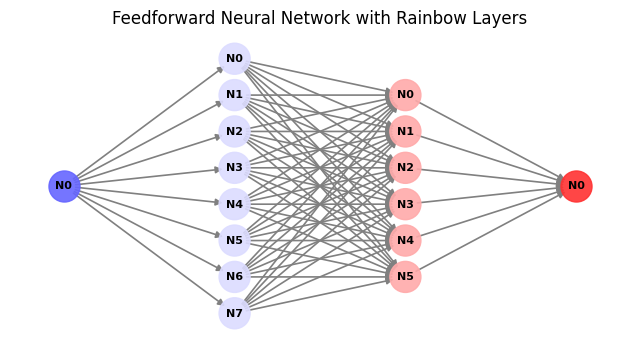
\includegraphics[width=0.7\textwidth]{images/feed_forward_network.png}
    \caption{Visualization of a simple Feedforward Neural Network (FFNN) with one hidden layer. The input, hidden, and output layers are aligned from left to right, with connections representing weight relationships.}
    \label{fig:feed_forward_network}
\end{figure}

\begin{codeonly}{Feed Forward Network}
import torch
import torch.nn as nn
import torch.optim as optim

# Define a deeper FFNN with two hidden layers
class FeedForwardNN(nn.Module):
    def __init__(self, input_size, hidden_size1, hidden_size2, output_size):
        super(FeedForwardNN, self).__init__()
        self.fc1 = nn.Linear(input_size, hidden_size1)
        self.relu1 = nn.ReLU()
        self.fc2 = nn.Linear(hidden_size1, hidden_size2)
        self.relu2 = nn.ReLU()
        self.fc3 = nn.Linear(hidden_size2, output_size)

    def forward(self, x):
        x = self.fc1(x)
        x = self.relu1(x)
        x = self.fc2(x)
        x = self.relu2(x)
        x = self.fc3(x)
        return x

# Create a model instance with 1 input, 8 neurons in the first hidden layer, 
# 6 neurons in the second hidden layer, and 1 output
input_size, hidden_size1, hidden_size2, output_size = 1, 8, 6, 1
model = FeedForwardNN(input_size, hidden_size1, hidden_size2, output_size)

# Print model architecture
print(model)
\end{codeonly}

A feedforward neural network (FFNN) consists of layers of interconnected neurons that transform input data into predictions. In this implementation, the network has an input layer with one neuron, two hidden layers with eight and six neurons, respectively, and an output layer with a single neuron. Each hidden layer applies a ReLU activation function to introduce non-linearity, enabling the model to learn complex relationships. The final output layer performs a linear transformation. 

The weights and biases of the network are learned during training through backpropagation, minimizing a chosen loss function. PyTorch's `nn.Linear` modules define fully connected layers, while the `forward` method specifies how data flows through the network. The model instance is created with predefined input, hidden, and output dimensions, and printing it reveals its architecture.

We now use such a feedforward network to approximate a non-linear curve. 

\begin{codeonly}{Learning a curve with FFNN}
import torch
import torch.nn as nn
import torch.optim as optim
import numpy as np
import matplotlib.pyplot as plt

# Set random seed & generate data: f(x) = 1 / (1 + exp(-tau * x + s))
torch.manual_seed(42); np.random.seed(42)
x = np.linspace(-2, 2, 500)
y = 1 / (1 + np.exp(-5 * x))  # tau = 5, s = 0
x_tensor = torch.tensor(x, dtype=torch.float32).unsqueeze(1)
y_tensor = torch.tensor(y, dtype=torch.float32).unsqueeze(1)

# Define a deeper FFNN
class DeepFFNN(nn.Module):
    def __init__(self):
        super().__init__()
        self.fc1, self.fc2, self.fc3 = nn.Linear(1, 8), nn.Linear(8, 6), nn.Linear(6, 1)
    def forward(self, x): return self.fc3(torch.relu(self.fc2(torch.relu(self.fc1(x)))))

model = DeepFFNN()
criterion = nn.MSELoss()
optimizer = optim.Adam(model.parameters(), lr=0.01)

# Training
loss_history = []
for epoch in range(2000):
    optimizer.zero_grad()
    y_pred = model(x_tensor)
    loss = criterion(y_pred, y_tensor)
    loss.backward()
    optimizer.step()
    loss_history.append(loss.item())
    if (epoch + 1) % 500 == 0: print(f"Epoch {epoch+1}, Loss: {loss.item():.6f}")

# Generate predictions
with torch.no_grad(): y_pred_np = model(x_tensor).numpy()

# Plot function approximation & loss curve
fig, axes = plt.subplots(1, 2, figsize=(10, 3))
axes[0].plot(x, y, label="True", linewidth=2)
axes[0].plot(x, y_pred_np, "r--", label="NN Approx.", linewidth=2)
axes[0].set(title="Function Approximation", xlabel="x", ylabel="f(x)"); axes[0].legend(); axes[0].grid()
axes[1].semilogy(loss_history, "r", label="Loss")
axes[1].set(title="Loss Curve", xlabel="Epochs", ylabel="MSE"); axes[1].legend(); axes[1].grid()
plt.savefig("deep_nn_results.png")
plt.show()
\end{codeonly}

\begin{figure}[ht]
    \centering
    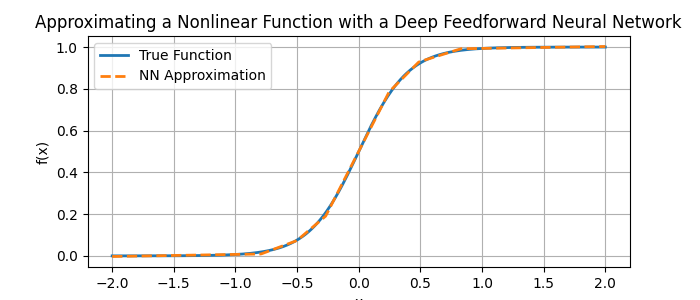
\includegraphics[width=0.48\textwidth]{images/deep_nn_function_approximation.png}
    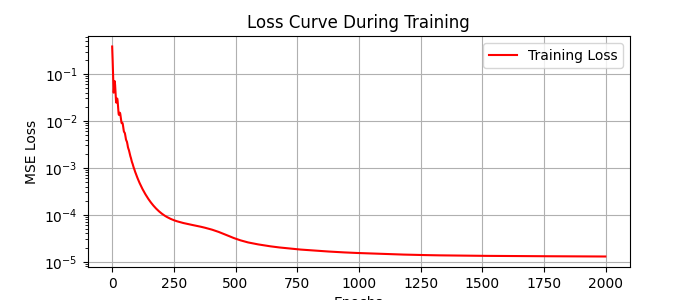
\includegraphics[width=0.48\textwidth]{images/deep_nn_loss_curve.png}
    \caption{Left: Neural network approximation of the function \( f(x) = \frac{1}{1 + e^{-\tau x + s}} \). 
    Right: Training loss curve over epochs, showing convergence of the model.}
    \label{fig:nn_function_loss}
\end{figure}

A computational graph visually represents how data flows through a neural network during a forward pass. In this example, we use the \texttt{torchviz} library to generate a graph of the feedforward neural network (FFNN). The input tensor is a randomly generated vector with the same dimensionality as the input layer. The forward pass computes the predicted output, which is then passed to \texttt{make\_dot()} along with the model’s parameters. The resulting graph shows the dependencies between layers and operations, helping to analyze the network structure and gradient flow.

\begin{codeonly}{Generating a Computational Graph}
from torchviz import make_dot

# Sample input tensor (random data)
x = torch.randn(1, input_size)  # One sample with 1 feature
y_pred = model(x)  # Forward pass

# Create the computational graph
dot = make_dot(y_pred, params=dict(model.named_parameters()))

# Render the graph
dot.render("ffnn_graph", format="png", cleanup=True)
dot
\end{codeonly}

\begin{figure}
    \centering
    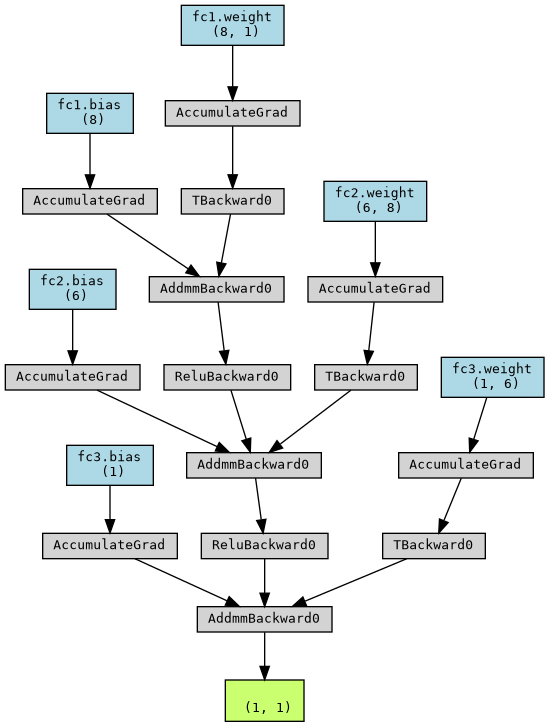
\includegraphics[width=0.6\textwidth]{images/ffnn_graph.png}
    \caption{Computational graph of the feedforward neural network.}
\end{figure}

Each box in the computational graph represents a tensor operation within the neural network. The nodes labeled \textbf{Addmm} correspond to the linear transformations performed by the \texttt{nn.Linear} layers, which compute matrix multiplications followed by bias addition. The \textbf{Relu} nodes apply the ReLU activation function, introducing non-linearity into the network. 

The parameters of the network, such as weights and biases, are indicated separately and contribute to the forward computation. This visualization helps trace how data propagates through the layers and identifies where gradients will be computed during backpropagation.

In the computational graph, \textbf{Accumulated Grad} represents the storage of gradients during backpropagation. When computing the gradient of the loss with respect to model parameters, PyTorch accumulates these gradients in the \texttt{.grad} attribute of tensors, allowing optimization steps to adjust weights accordingly.

\textbf{AddmmBackward} corresponds to the backward operation of the \textbf{Addmm} function, which performs matrix multiplication followed by bias addition in the forward pass. During backpropagation, \textbf{AddmmBackward} computes the gradients of the output with respect to both the input features and the weight matrices of the fully connected layers. These gradients are then accumulated and used for parameter updates during training.

%==============================================================================
%
%==============================================================================
\section{Graph Neural Networks}

Graph Neural Networks (GNNs) are designed to work with graph-structured data. Unlike FFNNs, GNNs can capture relationships between different entities in a graph, making them useful in applications such as social network analysis, molecular property prediction, and recommendation systems.

\begin{figure}[h!]
    \centering
    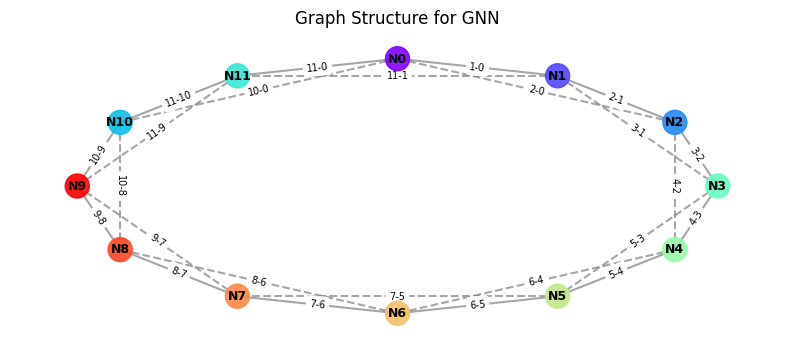
\includegraphics[width=0.8\textwidth]{images/gnn_graph.png}
    \caption{Graph visualization for the GNN model with periodic connectivity and elliptical node positions. The nodes are positioned on an ellipse, and the edges are displayed with two types: straight edges (direct neighbors) and periodic edges (non-direct neighbors).}
    \label{fig:gnn_graph}
\end{figure}

A simple implementation using PyTorch Geometric is shown below. I could get this easily running on linux, on my windows wls, on colab and other frameworks, but on Windows it died regularly without error message. Seems to be a memory management problem. 

\begin{recommendationbox}
Training with pytorch or pytorch lightning packages or any other current AI/ML software is characterized by frequent software updates. You will need to move along with the community in a timescale of month, packages get depreciated soon. 
\end{recommendationbox}

\begin{codeonly}{Graph Neural Network}
import torch
import torch.nn as nn
import torch.nn.functional as F
from torch_geometric.nn import GCNConv
from torch_geometric.data import Data

# Define a GNN with 2 hidden layers
class GNNModel(nn.Module):
    def __init__(self, num_features, hidden_channels, num_feats_y):
        super().__init__()
        self.conv1, self.conv2 = GCNConv(num_features, hidden_channels[0]), GCNConv(hidden_channels[0], hidden_channels[1])
        self.fc1, self.fc2 = nn.Linear(hidden_channels[1], hidden_channels[0]), nn.Linear(hidden_channels[0], num_feats_y)

    def forward(self, x, edge_index):
        x = F.leaky_relu(self.conv1(x, edge_index))
        x = F.leaky_relu(self.conv2(x, edge_index))
        x = F.leaky_relu(self.fc1(x))
        return self.fc2(x)

# Graph Configuration
nx, xa = 25, 10
x_grid = torch.linspace(0, xa, nx)
p1, p2 = torch.sin(2 * torch.pi * x_grid / xa), torch.cos(2 * torch.pi * x_grid / xa)

# Create adjacency matrix & edge index
diff = torch.sqrt((p1.repeat(nx, 1).T - p1) ** 2 + (p2.repeat(nx, 1).T - p2) ** 2)
edge_index = (diff < 0.5).float().nonzero(as_tuple=False).t().contiguous()

# Create node features & labels
data = Data(x=torch.cat((p1.unsqueeze(1), p2.unsqueeze(1)), dim=1), y=torch.randint(0, 2, (nx, 1)).float(), edge_index=edge_index)

# Initialize & print model
model = GNNModel(num_features=2, hidden_channels=[8, 16], num_feats_y=1)
print(model)
\end{codeonly}

Here, the edge index is for each node given by its index (first row) it prescribes the connected node by index in the second row.  
\begin{codeonly}{edge\_index}
tensor([[ 0,  0,  0,  0,  1,  1,  1,  1,  2,  2,  2,  2,  3,  3,  3,  3,  4,  4,
          4,  4,  5,  5,  5,  5,  6,  6,  6,  6,  7,  7,  7,  7,  8,  8,  8,  8,
          9,  9,  9,  9, 10, 10, 10, 10, 11, 11, 11, 11],
        [ 1,  2, 10, 11,  0,  2,  3, 11,  0,  1,  3,  4,  1,  2,  4,  5,  2,  3,
          5,  6,  3,  4,  6,  7,  4,  5,  7,  8,  5,  6,  8,  9,  6,  7,  9, 10,
          7,  8, 10, 11,  0,  8,  9, 11,  0,  1,  9, 10]])
\end{codeonly}

\begin{figure}[h!]
    \centering
    \begin{minipage}{0.45\textwidth}
        \centering
        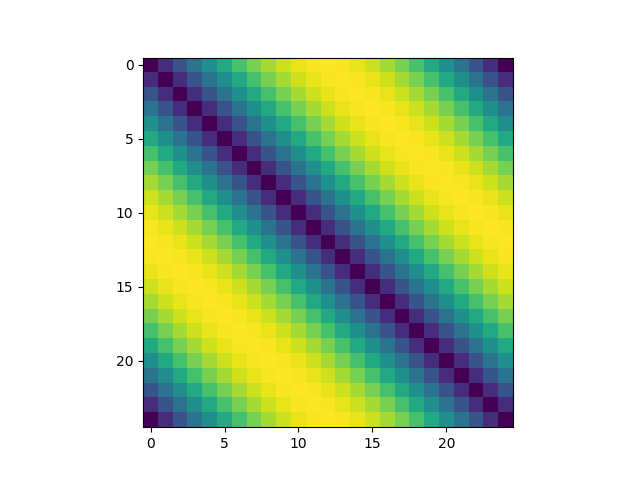
\includegraphics[width=\textwidth]{images/diff_matrix.png}
        \caption{The difference matrix showing the distances between nodes in the graph. This matrix is used to determine the adjacency matrix, where the distance between nodes is calculated based on their positions in the space.}
        \label{fig:diff_matrix}
    \end{minipage} \hfill
    \begin{minipage}{0.45\textwidth}
        \centering
        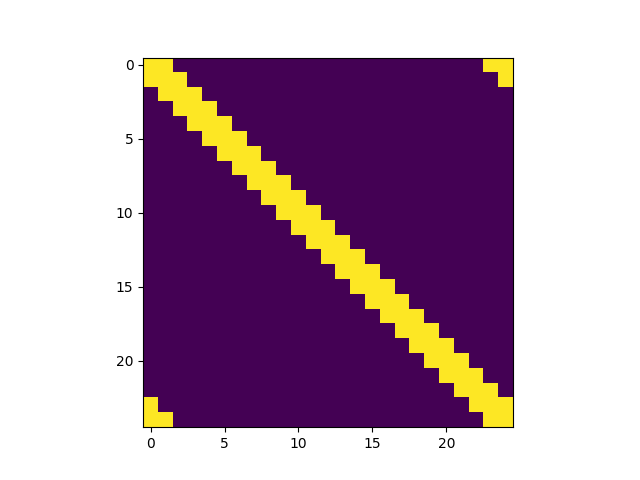
\includegraphics[width=\textwidth]{images/diff_matrix_smaller_const.png}
        \caption{A binary adjacency matrix where edges are drawn between nodes whose distance is less than 0.5. This matrix is used to determine which nodes are directly connected in the graph.}
        \label{fig:diff_matrix_smaller}
    \end{minipage}
\end{figure}

We finally show how we can learn the {\bf advection} of functions by a the above graph neural network. 

\begin{codeonly}{Training code}
import numpy as np
import matplotlib.pyplot as plt
import torch
import torch.nn as nn
import torch.nn.functional as F
import torch_geometric.data as geom_data
import torch_geometric.nn as geom_nn

# Set random seed
torch.manual_seed(0)

# Define parameters
xa, nx, nt, v = 10, 25, 15, 0.6

# Create grid and function data
x_grid = np.linspace(0, xa, nx + 1)[:-1]
z = np.zeros([nt, nx])
for j in range(nt):
    z[j, :] = np.sin((2 * np.pi / xa) * x_grid - v * j)

# Create adjacency matrix
p1 = np.sin(2 * np.pi * x_grid / xa)
p2 = np.cos(2 * np.pi * x_grid / xa)
p1m, p2m = np.tile(p1, (nx, 1)).T, np.tile(p2, (nx, 1)).T
diff = np.sqrt((p1m - p1m.T) ** 2 + (p2m - p2m.T) ** 2)
adjm = (diff < 0.5).astype(int)
edge_index = torch.tensor(np.nonzero(adjm), dtype=torch.long)

# Split data into training and testing
X_train, Y_train = z[:-1], z[1:]
X_test, Y_test = z[:-1], z[1:]

# Create feature tensors and data loader
features_tmp2 = torch.tensor(np.arange(1, nx + 1) / nx, dtype=torch.float).unsqueeze(1)
train_list, test_list = [], []
for k in range(X_train.shape[0]):
    features_k_tmp1 = torch.tensor(X_train[k, :], dtype=torch.float).unsqueeze(1)
    features_k = torch.cat((features_k_tmp1, features_tmp2), dim=1)
    labels_k = torch.tensor(Y_train[k, :], dtype=torch.float).unsqueeze(1)
    data = geom_data.Data(x=features_k, y=labels_k, edge_index=edge_index)
    train_list.append(data)

for k in range(X_test.shape[0]):
    features_k_tmp1 = torch.tensor(X_test[k, :], dtype=torch.float).unsqueeze(1)
    features_k = torch.cat((features_k_tmp1, features_tmp2), dim=1)
    labels_k = torch.tensor(Y_test[k, :], dtype=torch.float).unsqueeze(1)
    data = geom_data.Data(x=features_k, y=labels_k, edge_index=edge_index)
    test_list.append(data)

# Create DataLoaders for training and testing
train_loader = geom_data.DataLoader(train_list, batch_size=1, shuffle=True)
test_loader = geom_data.DataLoader(test_list, batch_size=1, shuffle=False)

# Define the GNN model
class GNNModel(nn.Module):
    def __init__(self, num_features, hidden_channels, num_feats_y):
        super(GNNModel, self).__init__()
        self.conv1 = geom_nn.GCNConv(num_features, hidden_channels[0])
        self.conv2 = geom_nn.GCNConv(hidden_channels[0], hidden_channels[1])
        self.conv3 = geom_nn.GCNConv(hidden_channels[1], hidden_channels[2])
        self.conv4 = geom_nn.GCNConv(hidden_channels[2], hidden_channels[3])
        self.fc1 = nn.Linear(hidden_channels[3], hidden_channels[2])
        self.fc2 = nn.Linear(hidden_channels[2], hidden_channels[0])
        self.fc3 = nn.Linear(hidden_channels[0], num_feats_y)

    def forward(self, x, edge_index):
        x = F.leaky_relu(self.conv1(x, edge_index))
        x = F.leaky_relu(self.conv2(x, edge_index))
        x = F.leaky_relu(self.conv3(x, edge_index))
        x = F.leaky_relu(self.conv4(x, edge_index))
        x = F.leaky_relu(self.fc1(x))
        x = F.leaky_relu(self.fc2(x))
        return self.fc3(x)

# Initialize model, optimizer, and criterion
model = GNNModel(num_features=2, hidden_channels=[4 * nt, 4 * nt, 4 * nt, 4 * nt], num_feats_y=1)
optimizer = torch.optim.AdamW(model.parameters(), lr=0.0005, weight_decay=0)
criterion = nn.MSELoss()

# Training loop
epochs = 1500
train_mse, test_mse = [], []
for epoch in range(epochs):
    model.train()
    total_loss = 0.0
    train_mse_tmp = []
    for batch in train_loader:
        optimizer.zero_grad()
        output = model(batch.x, batch.edge_index)
        loss = criterion(output, batch.y)
        train_mse_tmp.append(loss.item())
        loss.backward()
        optimizer.step()
    train_mse.append(np.mean(train_mse_tmp))

    model.eval()
    test_mse_tmp = []
    for batch in test_loader:
        y_pred = model(batch.x, batch.edge_index)
        test_loss = criterion(y_pred, batch.y)
        test_mse_tmp.append(test_loss.item())
    test_mse.append(np.mean(test_mse_tmp))

    if epoch % 100 == 0:
        print(f'Epoch {epoch + 1}, Train Loss: {train_mse[epoch]}, Test Loss: {test_mse[epoch]}')

# Plot training and test MSE
plt.plot(np.arange(epochs), train_mse, '*', label='Train Loss')
plt.plot(np.arange(epochs), test_mse, '*', label='Test Loss')
plt.legend()
plt.title("Training and Test Loss")
plt.savefig("gnn_loss_curve.png")
plt.show()
\end{codeonly}

Which comes with the loss curve

\begin{figure}[h!]
    \centering
    \begin{minipage}{0.8\textwidth}
        \centering
        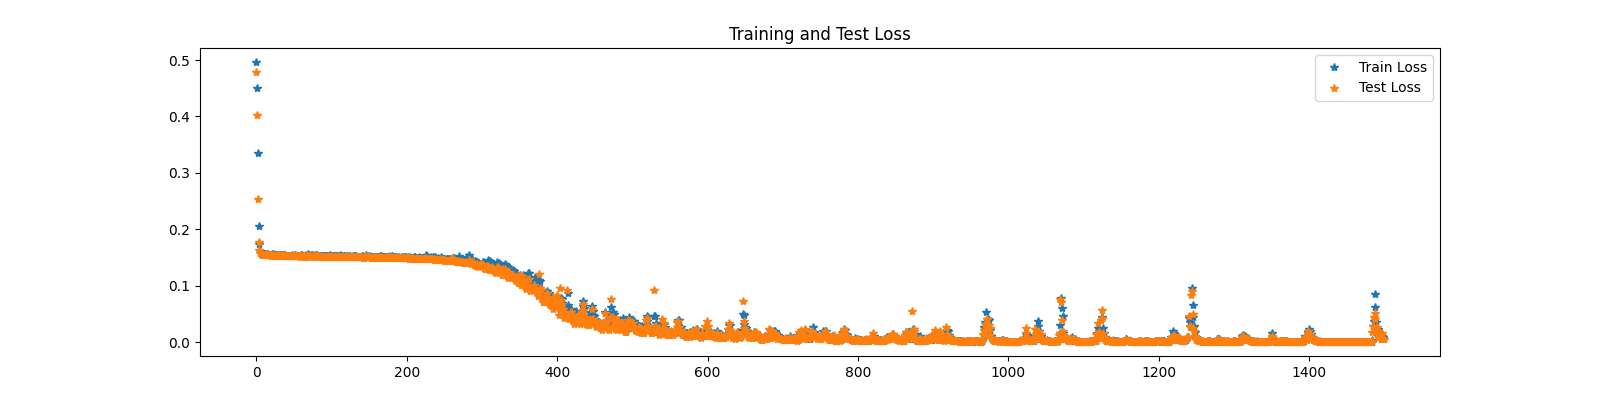
\includegraphics[width=\textwidth]{images/gnn_loss_curve.png}
        \caption{Training and Test Loss curves during the training process. The plot shows the Mean Squared Error (MSE) for both training and test sets across epochs.}
        \label{fig:gnn_test_2}
    \end{minipage}
\end{figure}

Testing the translation we display two randomly chosen cases. 

\begin{figure}[h!]
    \centering
    \begin{minipage}{0.45\textwidth}
        \centering
        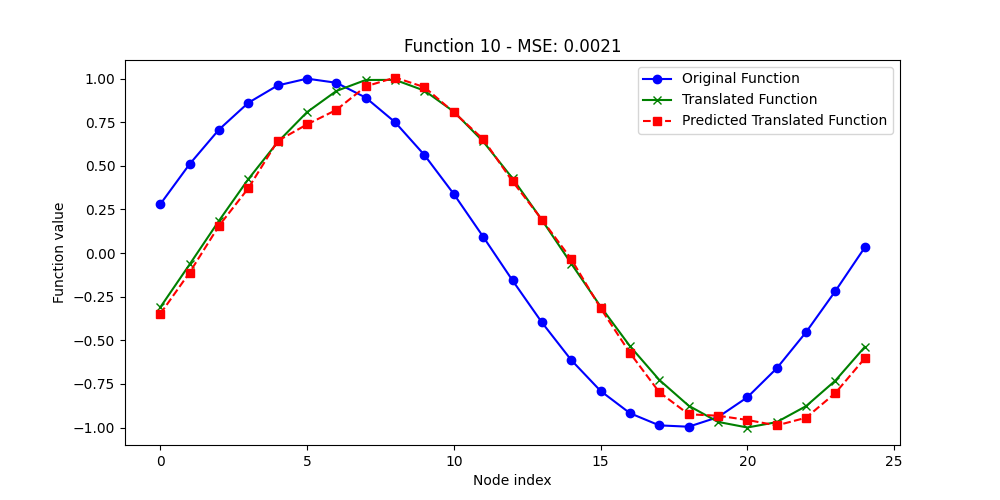
\includegraphics[width=\textwidth]{images/gnn_test_tds_1.png}
        \caption{Comparison for Test Case 1: Original, Translated, and Predicted Translated Functions. The plot shows the original function, the translated function, and the model's prediction with MSE value.}
        \label{fig:gnn_loss_curve}
    \end{minipage} \hfill
    \begin{minipage}{0.45\textwidth}
        \centering
        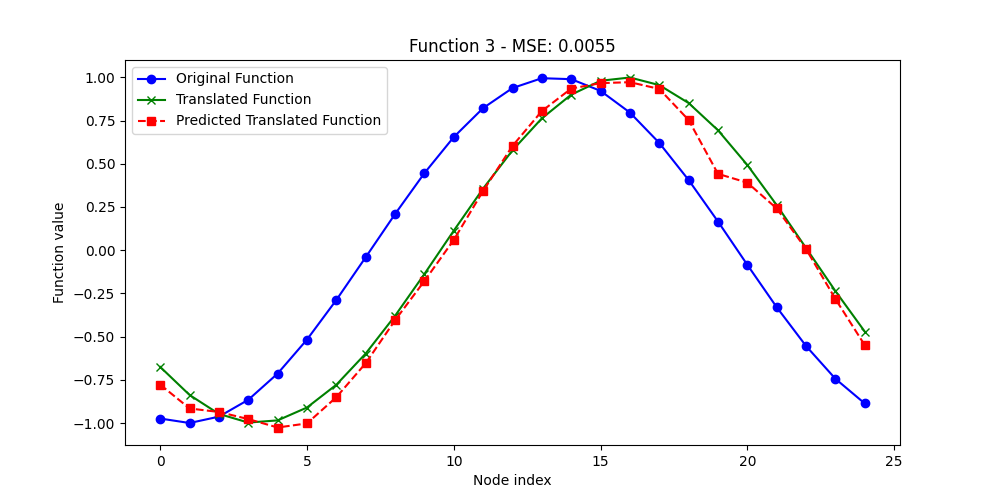
\includegraphics[width=\textwidth]{images/gnn_test_tds_2.png}
        \caption{Comparison for Test Case 2: Original, Translated, and Predicted Translated Functions. This plot compares the same as Test Case 1 but for another random test case.}
        \label{fig:gnn_test_1}
    \end{minipage}
\end{figure}



%==============================================================================
%
%==============================================================================
\section{Applying Convolutional Neural Networks for Function Classification}

Convolutional Neural Networks (CNNs) are powerful architectures typically used for image processing but can also be applied to one-dimensional data such as time series or function classification. In this section, we demonstrate how to construct a simple CNN to classify different mathematical functions (e.g., sine, cosine, Gaussian, and polynomial functions). 

{\bf Generating Synthetic Data.} To train a CNN, we first need a dataset. We generate synthetic data using functions such as sine or cosine, polynomials and Gaussians with varying parameters such as frequency, phase shifts, and noise levels. The dataset consists of labeled samples representing different mathematical function types. 

\begin{codeonly}{CNN Data generation}
import torch
import torch.nn as nn
import torch.optim as optim
import numpy as np
import matplotlib.pyplot as plt

def generate_function_data(num_samples=5000, num_points=50, err=0.02):
    X = []
    y = []
    functions = ['sine-cosine', 'gaussian', 'polynomial']
    
    for _ in range(num_samples):
        x = np.linspace(-1, 1, num_points)
        func_type = np.random.choice(functions)

        # Initialize a default y_values to prevent UnboundLocalError
        y_values = np.zeros(num_points)
        label = -1

        if func_type == 'sine-cosine':
            freq = np.random.uniform(1, 5)  
            phase = np.random.uniform(0, 2 * np.pi)
            amp = np.random.uniform(0.5, 2)
            y_values = amp * np.sin(freq * np.pi * x + phase) + err * np.random.randn(num_points)
            label = 0

        elif func_type == 'gaussian':
            mu = np.random.uniform(-0.5, 0.5)  
            sigma = np.random.uniform(0.2, 0.5)  
            amp = np.random.uniform(0.5, 2)
            y_values = amp * np.exp(-((x - mu) ** 2) / (2 * sigma ** 2)) + err * np.random.randn(num_points)
            label = 2

        elif func_type == 'polynomial':
            a = np.random.uniform(-2, 2)
            b = np.random.uniform(-2, 2)
            c = np.random.uniform(-3, 3)
            d = np.random.uniform(-0.5, 0.5)
            y_values = a * x**3 + b * x**2 + c * x + d + err * np.random.randn(num_points)
            label = 3

        X.append(y_values)
        y.append(label)

    X = np.array(X).reshape(-1, 1, num_points)  # Add channel dimension
    y = np.array(y)
    
    return torch.tensor(X, dtype=torch.float32), torch.tensor(y, dtype=torch.long)

# Generate a large training and test dataset with adjustable noise
X_train, y_train = generate_function_data(num_samples=10000, err=0.05)  # Low noise in training
X_test, y_test = generate_function_data(num_samples=2000, err=0.2)  # Higher noise in test set

print(f"Train Data Shape: {X_train.shape}, Train Labels Shape: {y_train.shape}")
print(f"Test Data Shape: {X_test.shape}, Test Labels Shape: {y_test.shape}")

plt.figure(figsize=(12, 3))
for i, idx in enumerate(torch.randperm(len(X_train))[:6]):
    plt.subplot(1, 6, i + 1)
    plt.plot(X_train[idx][0].cpu().numpy())
    plt.title([y_train[idx].item()])
    plt.xticks([]), plt.yticks([])

plt.tight_layout()
plt.savefig("cnn_data_samples.png", dpi=300)
plt.show()
\end{codeonly}
%\includeexternalcode{CNN Training Data}{chapter05/cnn_data_generation.py}

Each function is sampled over a fixed range, and the noise level can be controlled via a parameter. The generated dataset is split into training and test sets.

\begin{figure}[h]
    \centering
    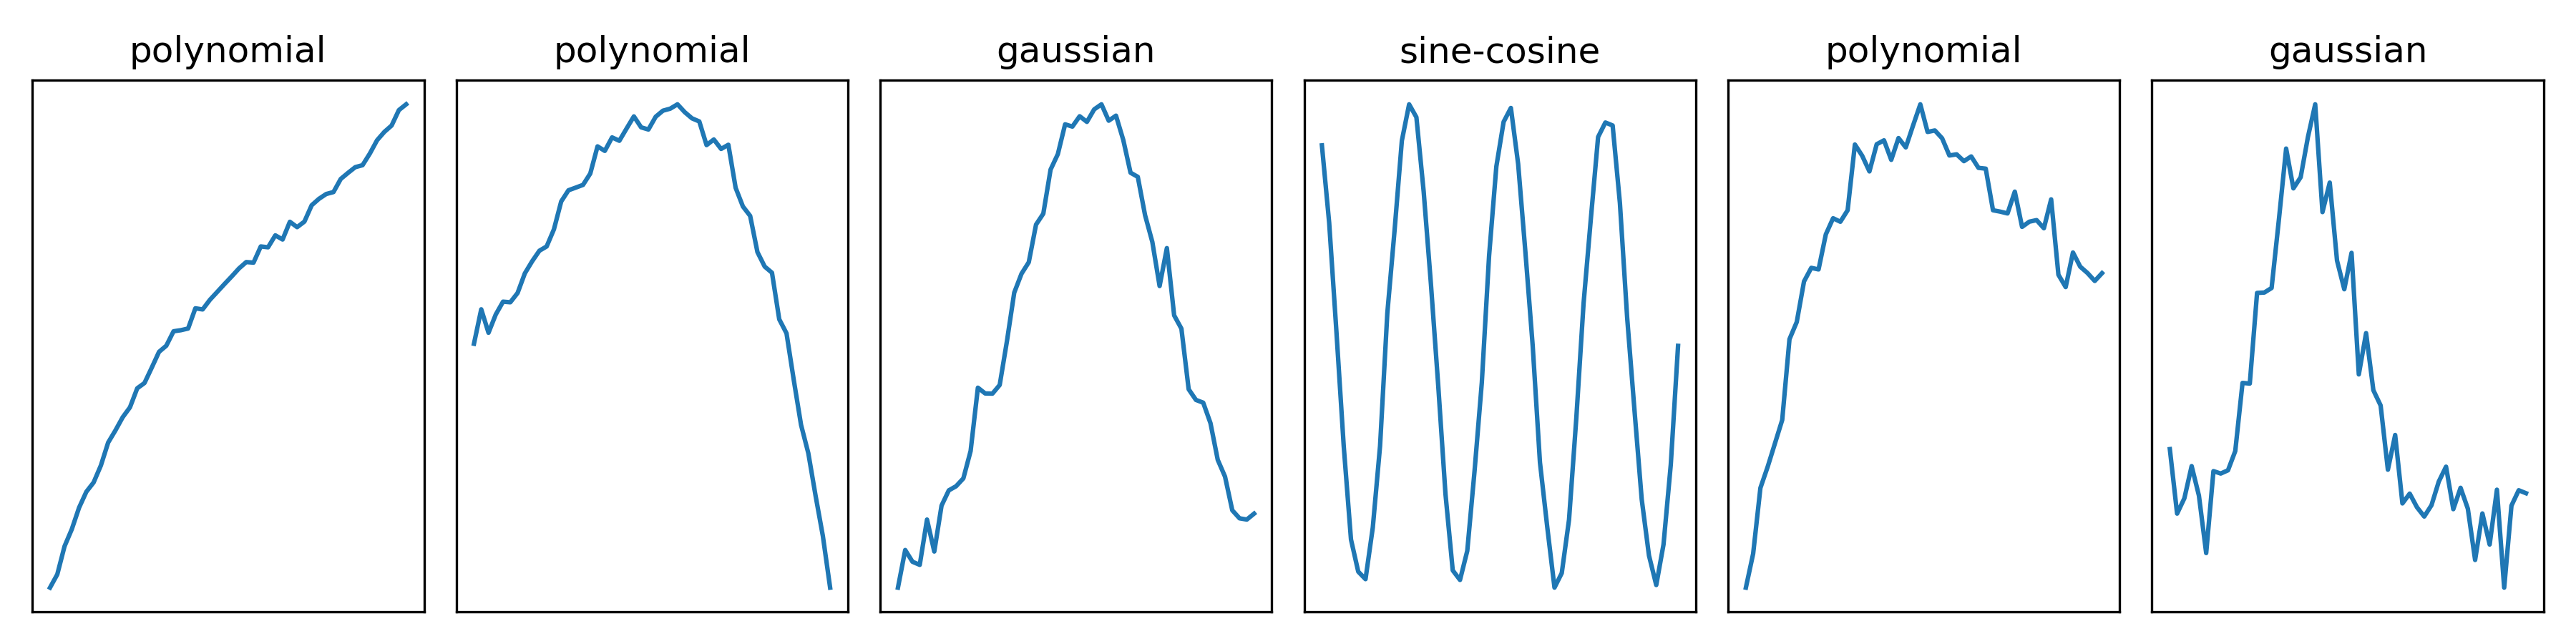
\includegraphics[width=0.8\textwidth]{images/cnn_data_samples_selected.png}
    \caption{Example of generated function data samples}
    \label{fig:data_samples}
\end{figure}

{\bf Defining the Convolutional Neural Network.} The next step is defining the CNN. Our model consists of two convolutional layers, followed by a fully connected network that maps extracted features to class labels.

\begin{codeonly}{CNN Definition}
import torch
import torch.nn as nn
import torch.optim as optim

class FunctionClassifierCNN(nn.Module):
    def __init__(self):
        super(FunctionClassifierCNN, self).__init__()
        self.conv1 = nn.Conv1d(in_channels=1, out_channels=16, kernel_size=5, stride=1, padding=2)
        self.conv2 = nn.Conv1d(in_channels=16, out_channels=32, kernel_size=5, stride=1, padding=2)
        self.fc1 = nn.Linear(32 * 50, 128)
        self.fc2 = nn.Linear(128, 4)  # 4 classes

    def forward(self, x):
        x = torch.relu(self.conv1(x))
        x = torch.relu(self.conv2(x))
        x = x.view(x.shape[0], -1)  # Flatten
        x = torch.relu(self.fc1(x))
        x = self.fc2(x)
        return x

# Initialize model
model = FunctionClassifierCNN()
print(model)
\end{codeonly}
%\includeexternalcode{CNN Definition}{chapter05/cnn_definition.py}

The convolutional layers apply feature extraction by detecting local patterns in the input functions. The final classification is performed by a fully connected layer.

{\bf Training the CNN.} The training process involves feeding the generated dataset into the CNN, computing loss using cross-entropy, and updating weights via backpropagation.

\begin{codeonly}{CNN Training}
# Training setup
device = torch.device("cuda" if torch.cuda.is_available() else "cpu")
model.to(device)

criterion = nn.CrossEntropyLoss()
optimizer = optim.Adam(model.parameters(), lr=0.001)

num_epochs = 20
batch_size = 32

# Convert dataset into DataLoader
train_loader = torch.utils.data.DataLoader(list(zip(X_train, y_train)), batch_size=batch_size, shuffle=True)

loss_history = []  # Store loss values

for epoch in range(num_epochs):
    total_loss = 0
    for batch_X, batch_y in train_loader:
        batch_X, batch_y = batch_X.to(device), batch_y.to(device)
        optimizer.zero_grad()
        loss = criterion(model(batch_X), batch_y)
        loss.backward()
        optimizer.step()
        total_loss += loss.item()
    
    loss_history.append(total_loss / len(train_loader))  # Save epoch loss
    print(f"Epoch {epoch+1}/{num_epochs}, Loss: {loss_history[-1]:.4f}")

# Plot training loss
fig=plt.figure(figsize=(10,5))
plt.plot(loss_history)
plt.xlabel("Epoch")
plt.ylabel("Loss")
plt.title("Training Loss")
plt.savefig("cnn_training_loss.png", dpi=300)
plt.show()
\end{codeonly}
%\includeexternalcode{CNN Training Loop}{chapter05/cnn_training.py}

During training, we monitor the loss function to ensure the model is learning effectively.

\begin{figure}[h]
    \centering
    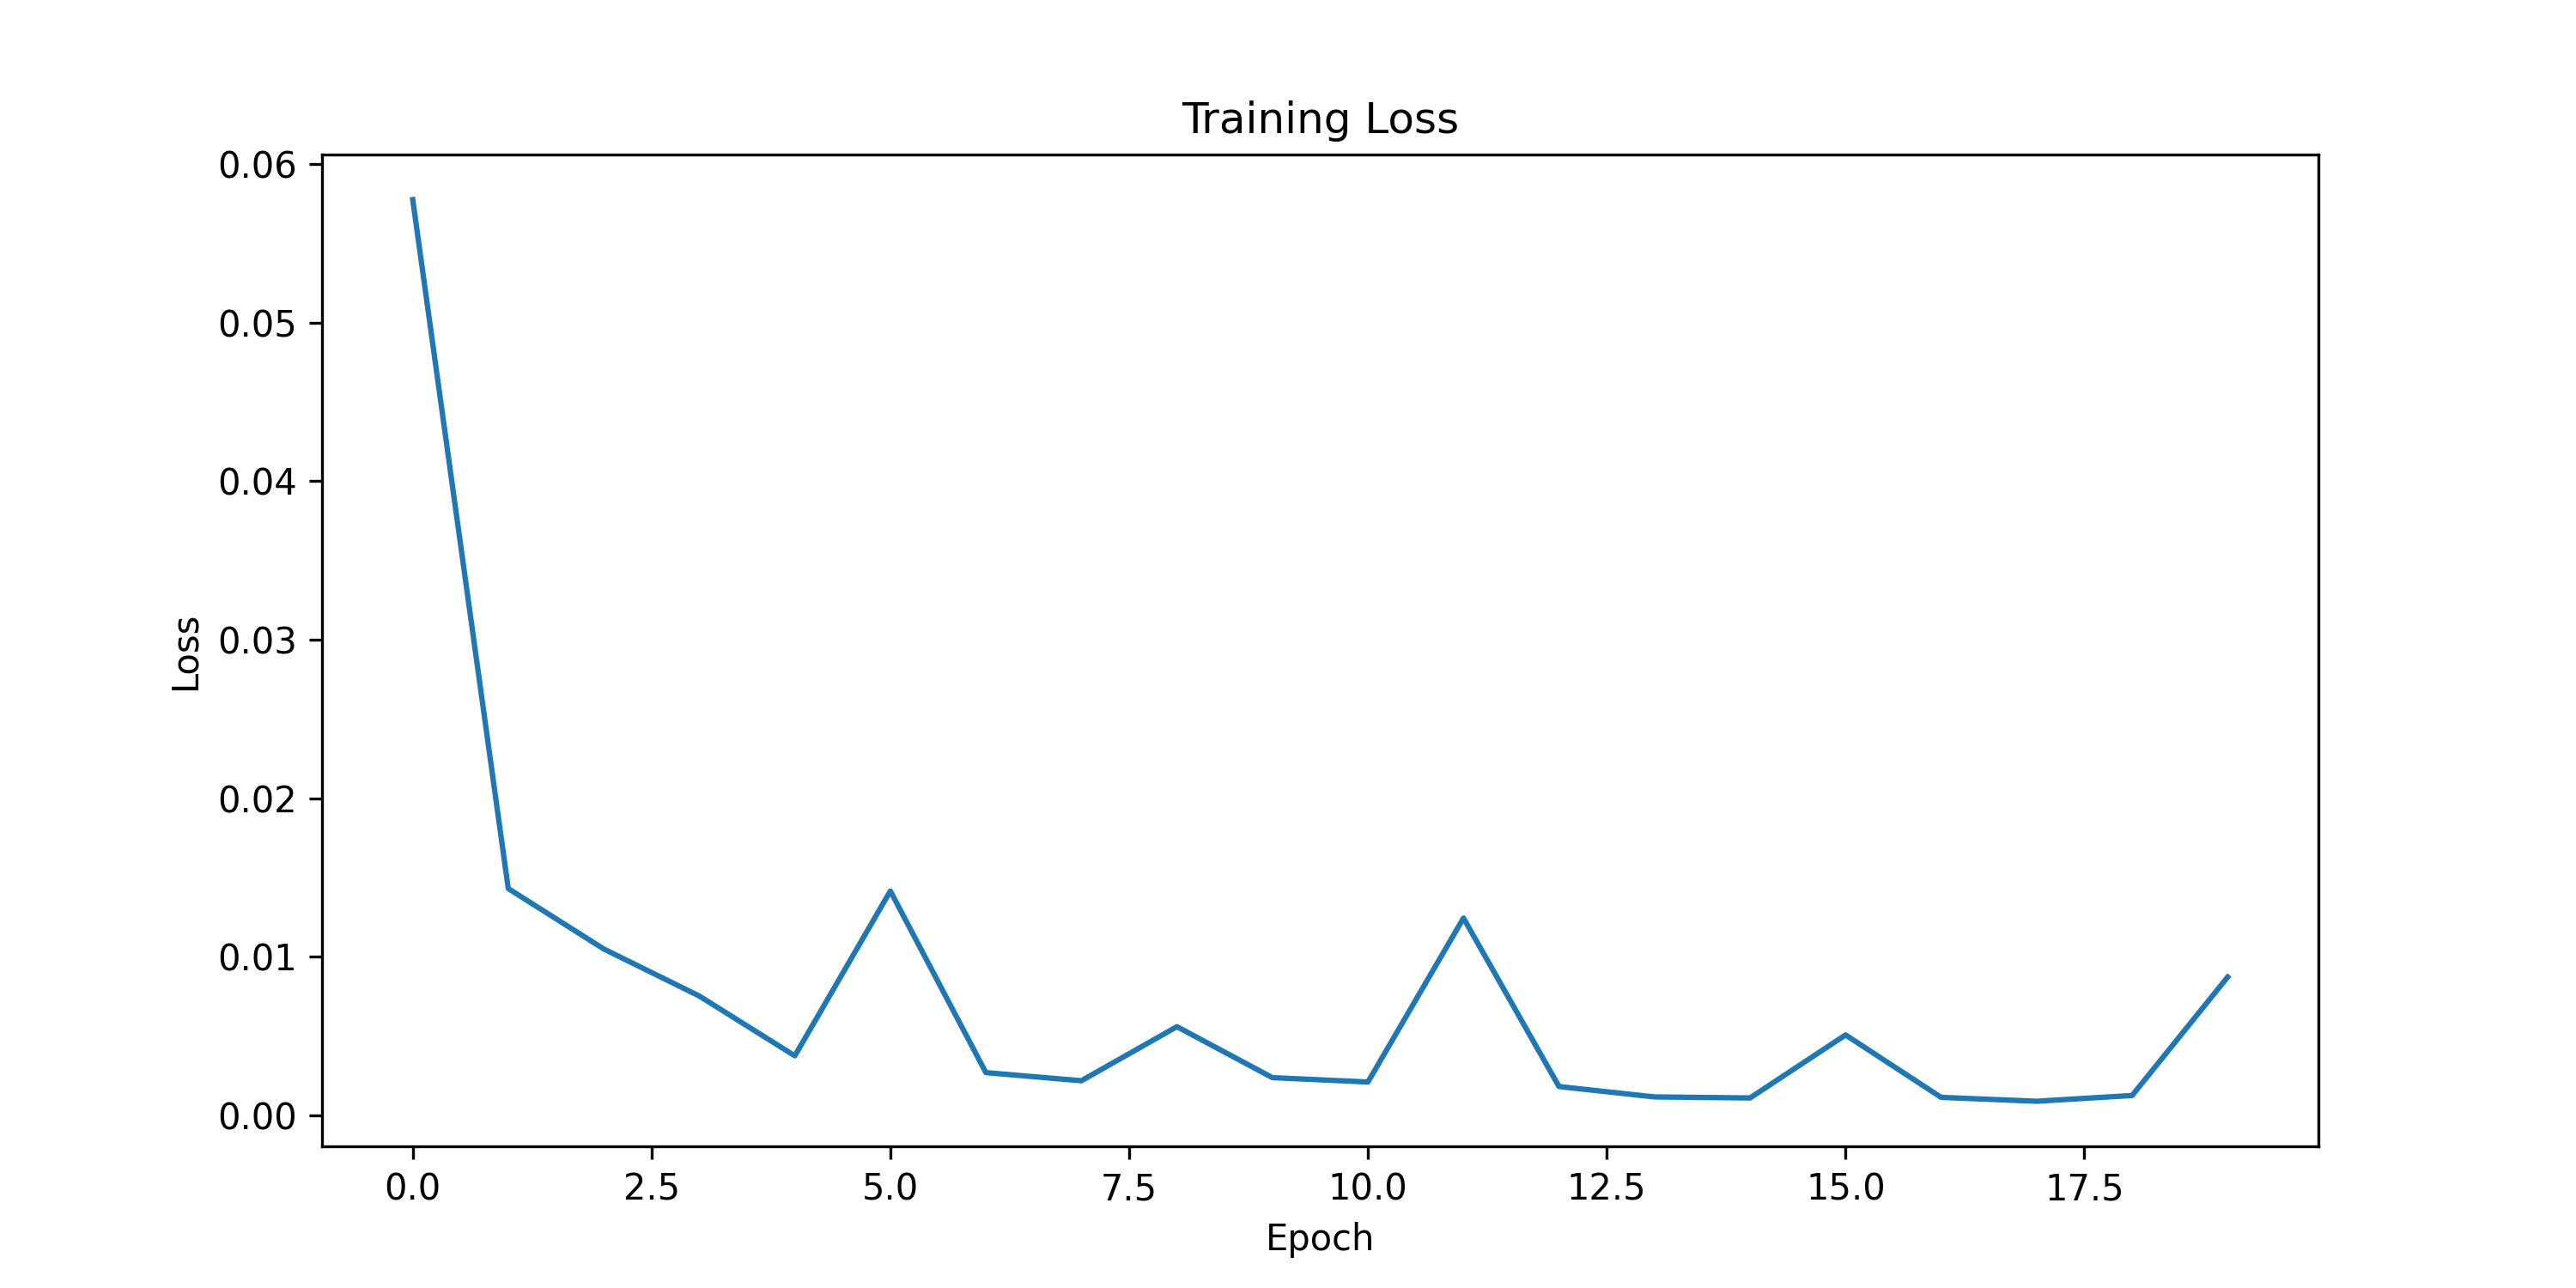
\includegraphics[width=0.8\textwidth]{images/cnn_training_loss.png}
    \caption{Training loss over epochs}
    \label{fig:training_loss}
\end{figure}

{\bf Evaluating the Model.} Once trained, the CNN is evaluated on the test dataset. Accuracy is computed to assess performance.

\begin{codeonly}{CNN Evaluation}
# Evaluation
model.eval()
test_loader = torch.utils.data.DataLoader(list(zip(X_test, y_test)), batch_size=batch_size, shuffle=False)

correct = 0
total = 0

with torch.no_grad():
    for batch_X, batch_y in test_loader:
        batch_X, batch_y = batch_X.to(device), batch_y.to(device)

        outputs = model(batch_X)
        _, predicted = torch.max(outputs, 1)

        total += batch_y.size(0)
        correct += (predicted == batch_y).sum().item()

accuracy = 100 * correct / total
print(f"Test Accuracy: {accuracy:.2f}%")
\end{codeonly}
%\includeexternalcode{Evaluation of CNN}{chapter05/cnn_evaluation.py}

A high accuracy indicates the model successfully differentiates between different function types.

{\bf Visualizing Predictions.} Finally, we visualize how well the model classifies unseen functions by plotting predicted and actual labels.

\begin{codeonly}{CNN Visualization}
import random
import matplotlib.pyplot as plt

# Generate a few test samples
num_examples = 12  # Show 12 examples
X_new, y_new = generate_function_data(num_samples=num_examples)
X_new = X_new.to(device)

# Get model predictions
model.eval()
with torch.no_grad():
    predictions = model(X_new)
    _, predicted_labels = torch.max(predictions, 1)

# Function names for visualization
func_names = ['Sine', 'Cosine', 'Gaussian', 'Polynomial']

# Plot the results
rows = num_examples // 4  # Show 4 per row
plt.figure(figsize=(12, 3 * rows))

for i in range(num_examples):
    correct = predicted_labels[i] == y_new[i]  # Check if prediction is correct
    color = 'blue' if correct else 'red'  # Blue for correct, red for incorrect

    plt.subplot(rows, 4, i + 1)
    plt.plot(np.linspace(-1, 1, 50), X_new[i].cpu().numpy().squeeze(), color=color, label=f"Pred: {func_names[predicted_labels[i]]}")
    plt.legend()
    plt.title(f"True: {func_names[y_new[i]]}", color=color)  # Color title for extra clarity
    plt.xticks([])
    plt.yticks([])

plt.tight_layout()
plt.savefig("cnn_test_predictions.png", dpi=300)
plt.show()
\end{codeonly}
%\includeexternalcode{CNN Result Visualization}{chapter05/cnn_visualization.py}

By analyzing the correctly and incorrectly classified samples, we can gain insights into model performance and potential improvements.

\begin{figure}[ht]
    \centering
    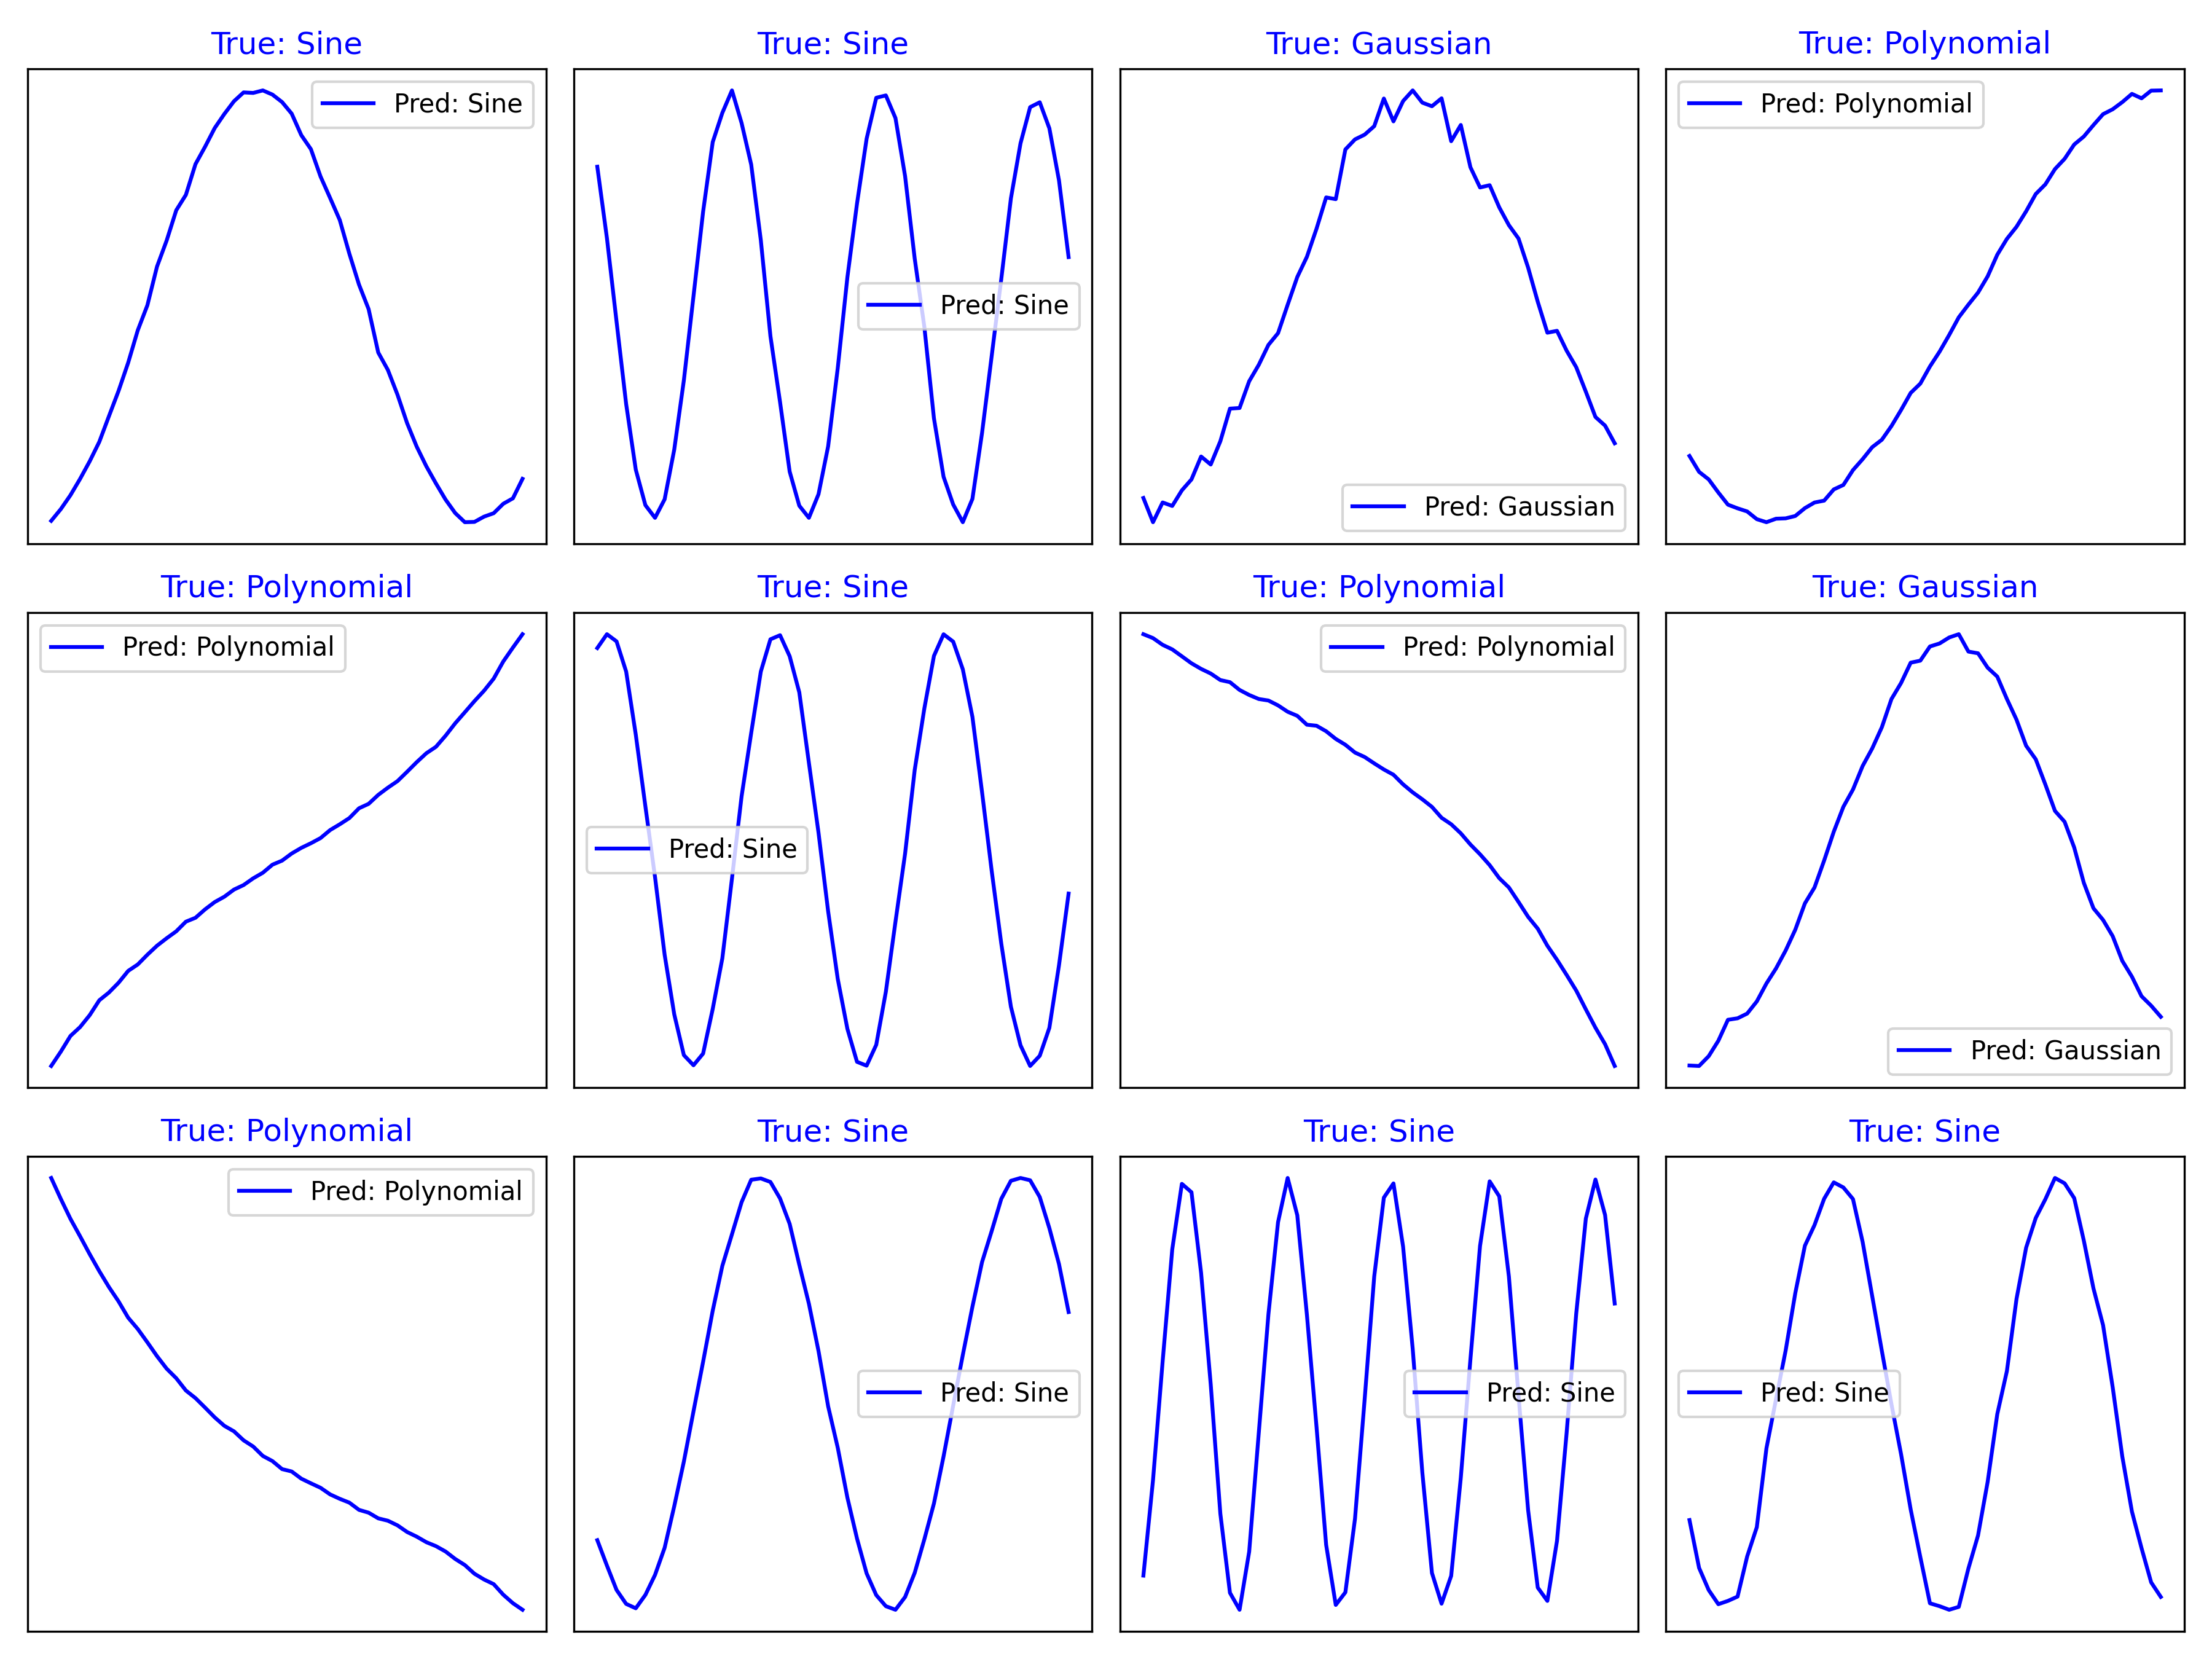
\includegraphics[width=0.8\textwidth]{images/cnn_test_predictions_select.png}
    \caption{Correct (blue) and incorrect (red) predictions}
    \label{fig:test_predictions}
\end{figure}

We have shown an application of CNNs for function classification, covering data generation, model design, training, evaluation, and visualization. This approach can be extended to classify other types of structured signals.

%==============================================================================
%
%==============================================================================
\section{LSTM-Based Anomaly Detection in Sensor Data}

Recurrent Neural Networks (RNNs), specifically Long Short-Term Memory (LSTM) networks, are powerful for handling sequential data. Unlike traditional feedforward neural networks, LSTMs are designed to capture temporal dependencies by maintaining an internal memory that allows them to remember relevant past information over long sequences. This makes them particularly suitable for anomaly detection in time series data, where deviations from learned patterns indicate potential anomalies.

An LSTM consists of a series of memory cells, each containing:
\begin{itemize}
    \item An \textbf{input gate} that determines how much new information is added to the cell state.
    \item A \textbf{forget gate} that decides what past information should be discarded.
    \item An \textbf{output gate} that controls how much information from the memory cell is used as output.
\end{itemize}
By adjusting these gates, the LSTM can selectively retain or forget information, making it highly effective at modeling sequences with long-term dependencies.

\begin{figure}[ht]
    \centering
    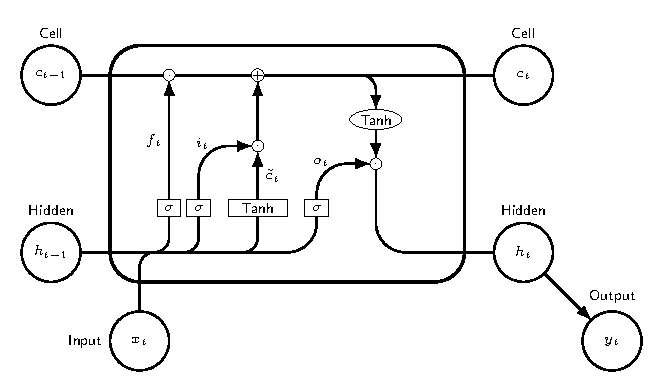
\includegraphics[width=0.6\textwidth]{chapters/lstm_graph.pdf}
    \caption{A sketch of the functionality of an LSTM cell, as described by the equations (\ref{lstm1})-(\ref{lstm7}). }
    \label{fig:lstm_graph}
\end{figure}

{\bf Mathematical Formulation of LSTM.} To be more precise, an LSTM unit consists of a cell state \( c_t \) and three gates: the input gate \( i_t \), forget gate \( f_t \), and output gate \( o_t \). The key equations governing an LSTM cell at time step \( t \) are:
\begin{eqnarray}
    f_t &= \sigma(W_f x_t + U_f h_{t-1} + b_f) \label{lstm1} \\
    i_t &= \sigma(W_i x_t + U_i h_{t-1} + b_i) \\
    o_t &= \sigma(W_o x_t + U_o h_{t-1} + b_o) \\
    \tilde{c}_t &= \tanh(W_c x_t + U_c h_{t-1} + b_c) \\
    c_t &= f_t \odot c_{t-1} + i_t \odot \tilde{c}_t \\
    h_t &= o_t \odot \tanh(c_t) \\
    y_t &= W_y h_t + b_y \label{lstm7}
\end{eqnarray}
following \href{https://arxiv.org/pdf/1506.04214}{Convolutional LSTM Network: A Machine Learning Approach for Precipitation Nowcasting}. 

Here, \( x_t \in \mathbb{R}^{m} \) represents the input at time step \( t \), while \( h_t \in \mathbb{R}^{n} \) is the hidden state, which encodes information from previous time steps. The memory cell \( c_t \in \mathbb{R}^{n} \) maintains long-term dependencies, with its update governed by three gates: the forget gate \( f_t \), which decides how much past information to retain, the input gate \( i_t \), which determines how much new information to store, and the output gate \( o_t \), which controls what is passed to the hidden state. The candidate cell state \( \tilde{c}_t \) contributes to updating \( c_t \), using weight matrices \( W_c \) and \( U_c \), and bias \( b_c \).

The weight matrices \( W_f, W_i, W_o, W_c \in \mathbb{R}^{n \times m} \) process input connections, while \( U_f, U_i, U_o, U_c \in \mathbb{R}^{n \times n} \) manage recurrent hidden state updates. Bias terms \( b_f, b_i, b_o, b_c \in \mathbb{R}^{n} \) adjust the activation functions. The element-wise sigmoid function \( \sigma \) regulates gate activations, and the hyperbolic tangent function \( \tanh \) is used for both candidate state computation and final output transformation. Element-wise multiplication is denoted by \( \odot \).

{\bf Output Computation.} The final output \( y_t \) is computed as a linear transformation \( W_y h_t + b_y \), where \( W_y \in \mathbb{R}^{p \times n} \) maps the hidden state to an output space of dimension \( p \), and \( b_y \in \mathbb{R}^{p} \) is the corresponding bias. The interpretation of \( y_t \) depends on the application: in sequence classification, \( y_t \) is typically taken from the final time step; in sequence-to-sequence tasks, it is used at every time step; and in autoencoders, it reconstructs the original sequence.

By updating these gates at each time step, LSTMs effectively address the vanishing gradient problem, enabling the learning of long-term dependencies in sequential data.


\bigskip
In this section, we implement an LSTM-based autoencoder to detect anomalies in simulated sensor data. The autoencoder learns to reconstruct normal sequences, and anomalies are detected based on high reconstruction error.

{\bf Generating Sensor Data.} 
To train the model, we generate synthetic sensor data using sine waves with random phase shifts. Anomalies are introduced as sudden deviations.

\begin{codeonly}{Generating Sensor Data}
import numpy as np

# Generate normal sine wave data with random phase shift
def generate_sensor_data(num_samples=1000, seq_length=50, anomaly_ratio=0.1):
    X = []
    labels = []

    for _ in range(num_samples):
        phase_shift = np.random.uniform(0, 2 * np.pi)  # Random shift
        time_series = np.sin(np.linspace(0, 2 * np.pi, seq_length) + phase_shift) + 0.1 * np.random.randn(seq_length)
        label = 0  # Normal

        # Inject anomalies
        if np.random.rand() < anomaly_ratio:
            time_series += np.random.uniform(-2, 2, size=seq_length)  # Add large spikes
            label = 1  # Anomaly

        X.append(time_series)
        labels.append(label)

    return np.array(X), np.array(labels)
\end{codeonly}

\begin{figure}[ht]
    \centering
    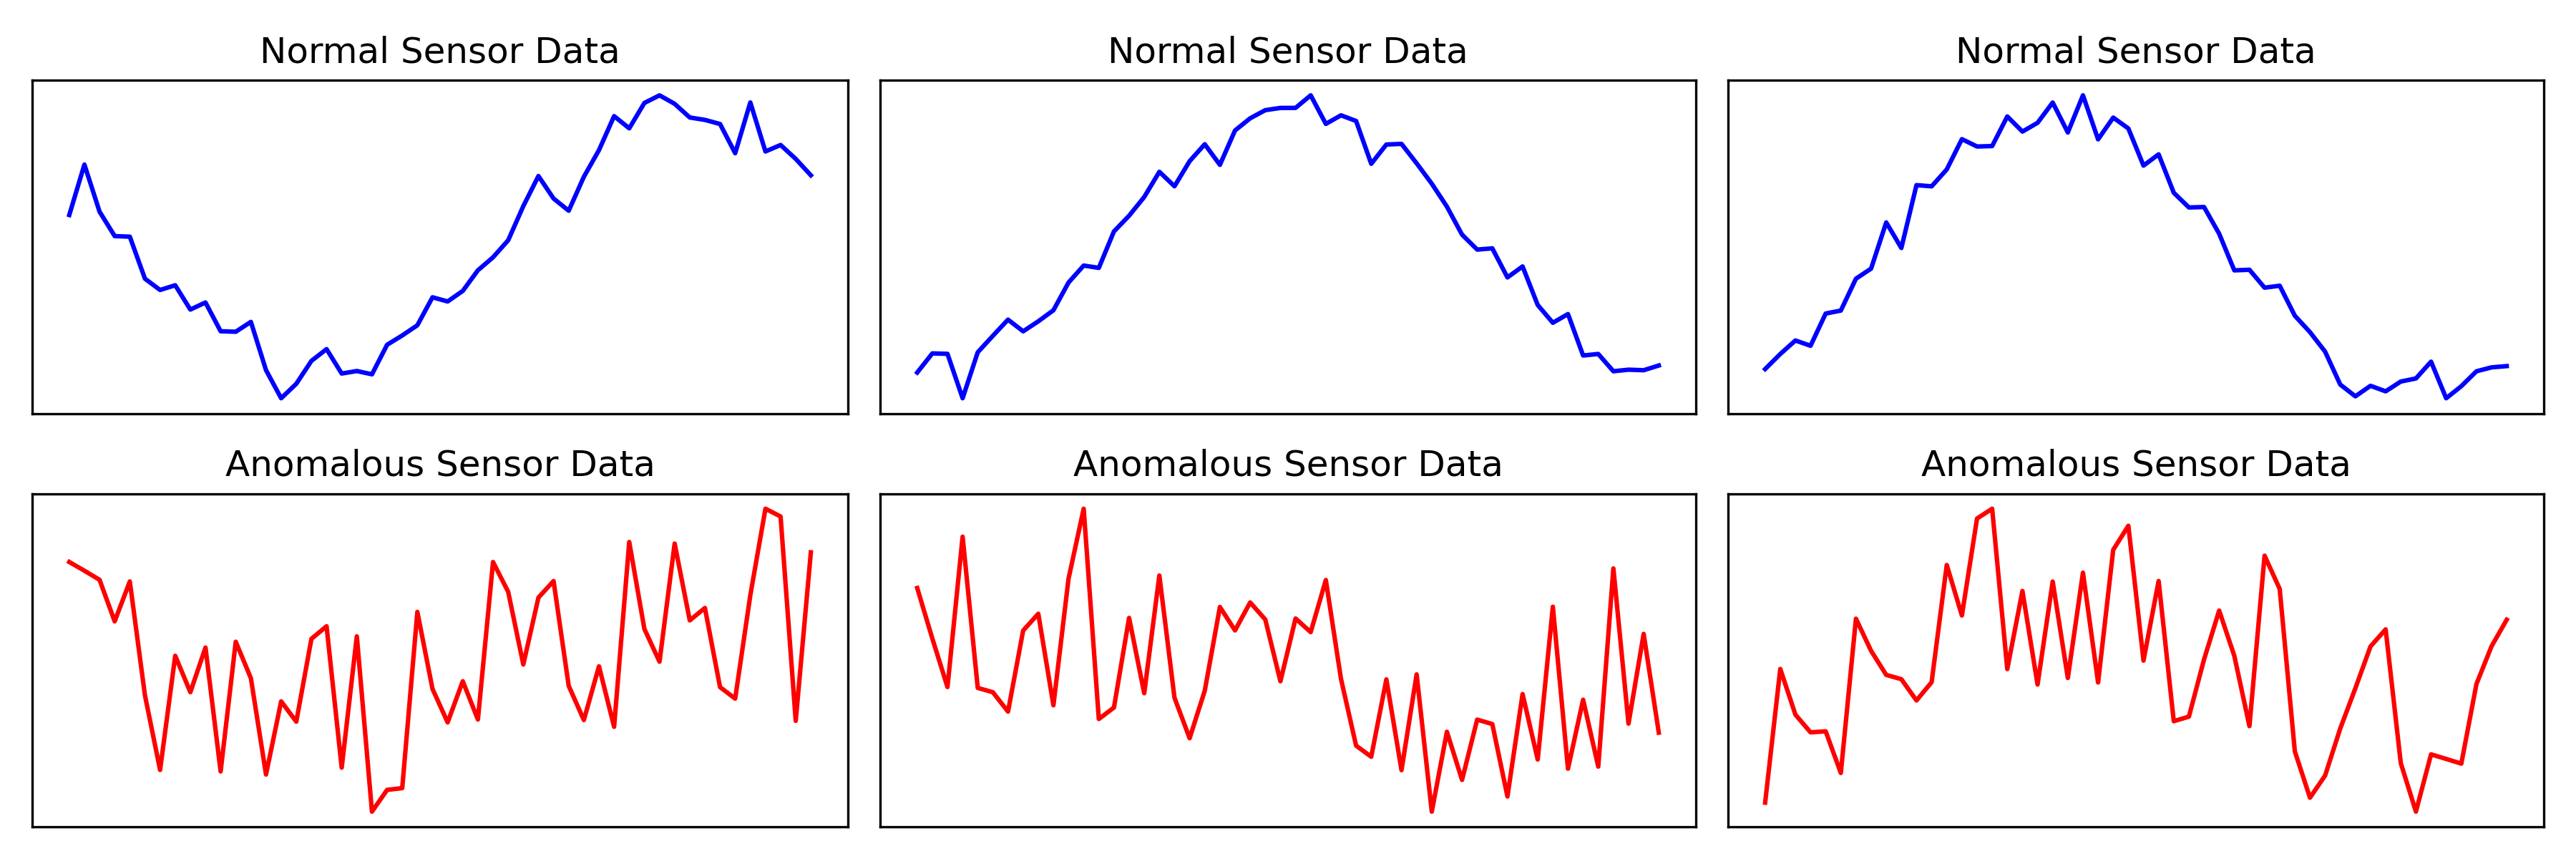
\includegraphics[width=0.9\textwidth]{images/lstm_sensor_data_samples.png}
    \caption{Examples of normal and anomalous sensor data. Normal sequences are in blue, while anomalies are shown in red.}
    \label{fig:sensor_data_samples}
\end{figure}

{\bf Defining the LSTM Autoencoder.} 
We define an LSTM autoencoder consisting of an encoder that compresses the input sequence into a lower-dimensional hidden state and a decoder that reconstructs the original sequence.

\begin{codeonly}{Defining the LSTM Autoencoder}
import torch

# Define device for computation (CPU/GPU)
device = torch.device("cuda" if torch.cuda.is_available() else "cpu")

class LSTMAutoencoder(nn.Module):
    def __init__(self, input_dim=1, hidden_dim=32, num_layers=2, seq_length=50):
        super(LSTMAutoencoder, self).__init__()
        self.seq_length = seq_length
        self.hidden_dim = hidden_dim
        self.num_layers = num_layers

        # LSTM layers
        self.encoder = nn.LSTM(input_dim,hidden_dim, num_layers,batch_first=True)
        self.decoder = nn.LSTM(input_dim,hidden_dim, num_layers,batch_first=True)

        # Final layer to reconstruct input
        self.output_layer = nn.Linear(hidden_dim, input_dim)

    def forward(self, x):
        batch_size = x.size(0)

        # Encode input
        _, (hidden, cell) = self.encoder(x)  # Correct hidden state extraction

        # Initialize decoder input as zeros
        decoder_input = torch.zeros(batch_size, self.seq_length, 1).to(x.device)

        # Decode using the last hidden state from the encoder
        decoder_output, _ = self.decoder(decoder_input, (hidden, cell))

        # Apply final layer to match original input size
        x_reconstructed = self.output_layer(decoder_output)

        return x_reconstructed  # Shape: [batch_size, seq_length, input_dim]

# Initialize model with correct sequence length
model = LSTMAutoencoder(seq_length=50).to(device)

\end{codeonly}

{\bf Training the Model.} 
The model is trained using Mean Squared Error (MSE) loss, optimizing the ability to reconstruct normal sequences.

\begin{codeonly}{Training the Model}
# Training setup
criterion = nn.MSELoss()
optimizer = optim.Adam(model.parameters(), lr=0.001)
num_epochs = 50
batch_size = 32

train_loader = torch.utils.data.DataLoader(X_train, batch_size=batch_size, shuffle=True)

# Track loss history
loss_history = []

# Training loop
for epoch in range(num_epochs):
    total_loss = 0
    for batch in train_loader:
        batch = batch.to(device)
        optimizer.zero_grad()
        outputs = model(batch)
        loss = criterion(outputs, batch)  # Compare input and output
        loss.backward()
        optimizer.step()
        total_loss += loss.item()

    epoch_loss = total_loss / len(train_loader)
    loss_history.append(epoch_loss)  # Store epoch loss
    print(f"Epoch {epoch+1}/{num_epochs}, Loss: {epoch_loss:.4f}")

plt.plot(loss_history, label="Loss")
plt.xlabel("Epochs"), plt.ylabel("Loss"), plt.title("LSTM Training Loss")
plt.legend(), plt.grid(True)
plt.savefig("lstm_training_loss.png", dpi=300)
plt.show()
\end{codeonly}

\begin{figure}[ht]
    \centering
    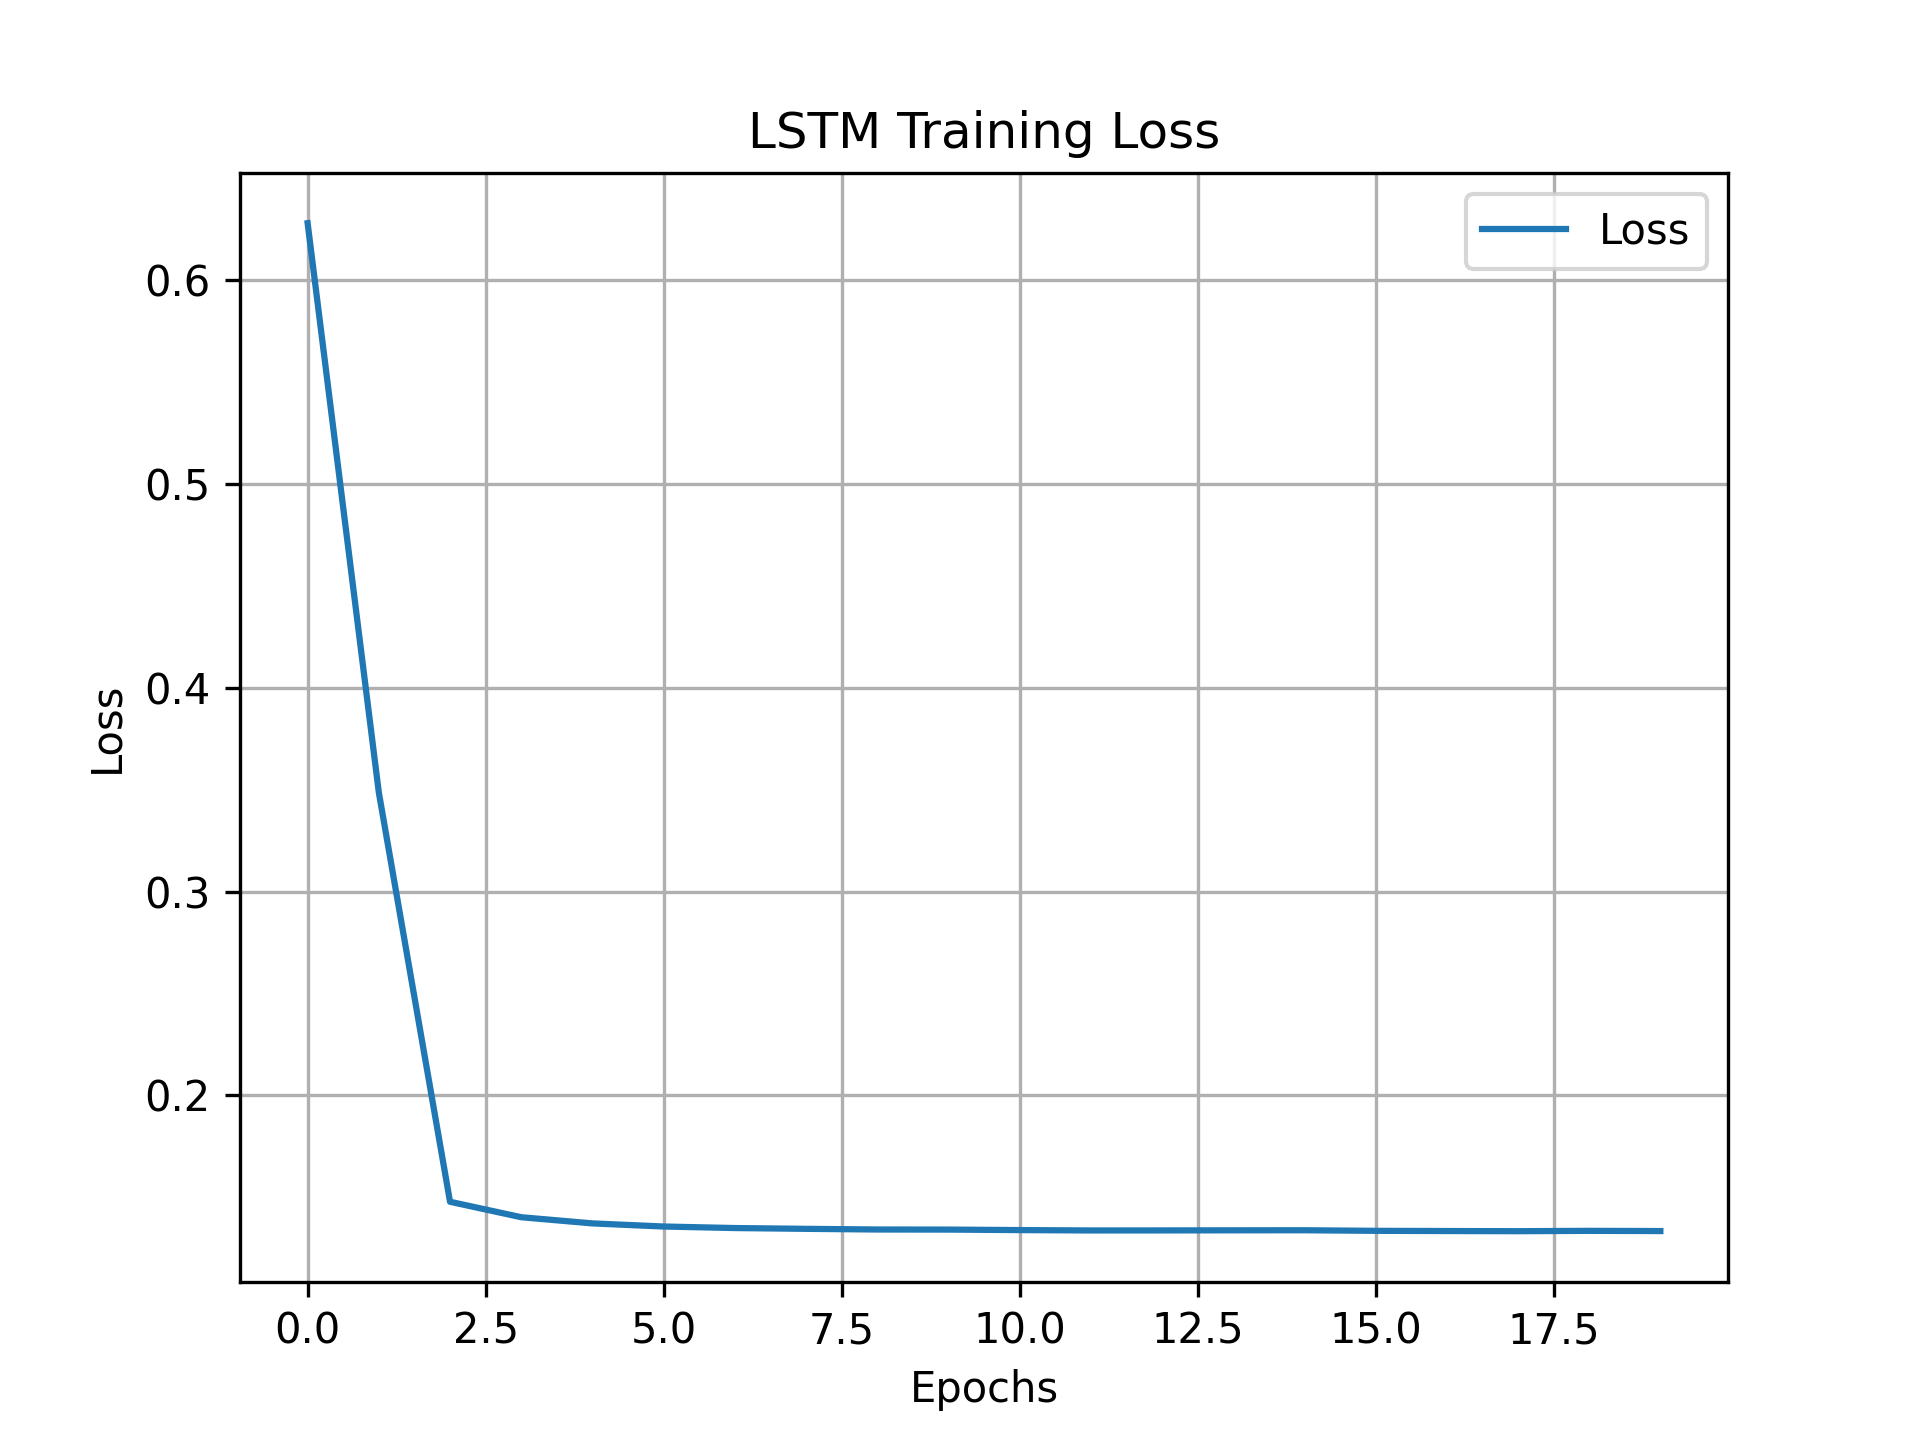
\includegraphics[width=0.9\textwidth]{images/lstm_training_loss.png}
    \caption{Training loss curve showing the decrease in reconstruction error over epochs.}
    \label{fig:training_loss}
\end{figure}

{\bf Detecting Anomalies.} 
Anomalies are detected by computing the reconstruction error on test sequences. If the error exceeds a predefined threshold (e.g., 95th percentile), the sequence is classified as an anomaly.

\begin{codeonly}{Anomaly Detection}
import numpy as np

# Compute reconstruction error on test data
model.eval()
X_test = X_test.to(device)
with torch.no_grad():
    X_reconstructed = model(X_test)

reconstruction_errors = torch.mean((X_test - X_reconstructed) ** 2, dim=(1, 2)).cpu().numpy()

# Set anomaly threshold (e.g., 95th percentile)
threshold = np.percentile(reconstruction_errors, 95)
y_pred = (reconstruction_errors > threshold).astype(int)  # 1 if anomaly, else 0

# Compute detection accuracy
accuracy = np.mean(y_pred == y_test) * 100
print(f"Anomaly Detection Accuracy: {accuracy:.2f}%")
\end{codeonly}

In our case we got 
\begin{verbatim}
Anomaly Detection Accuracy: 96.25%
\end{verbatim}

\begin{figure}[ht]
    \centering
    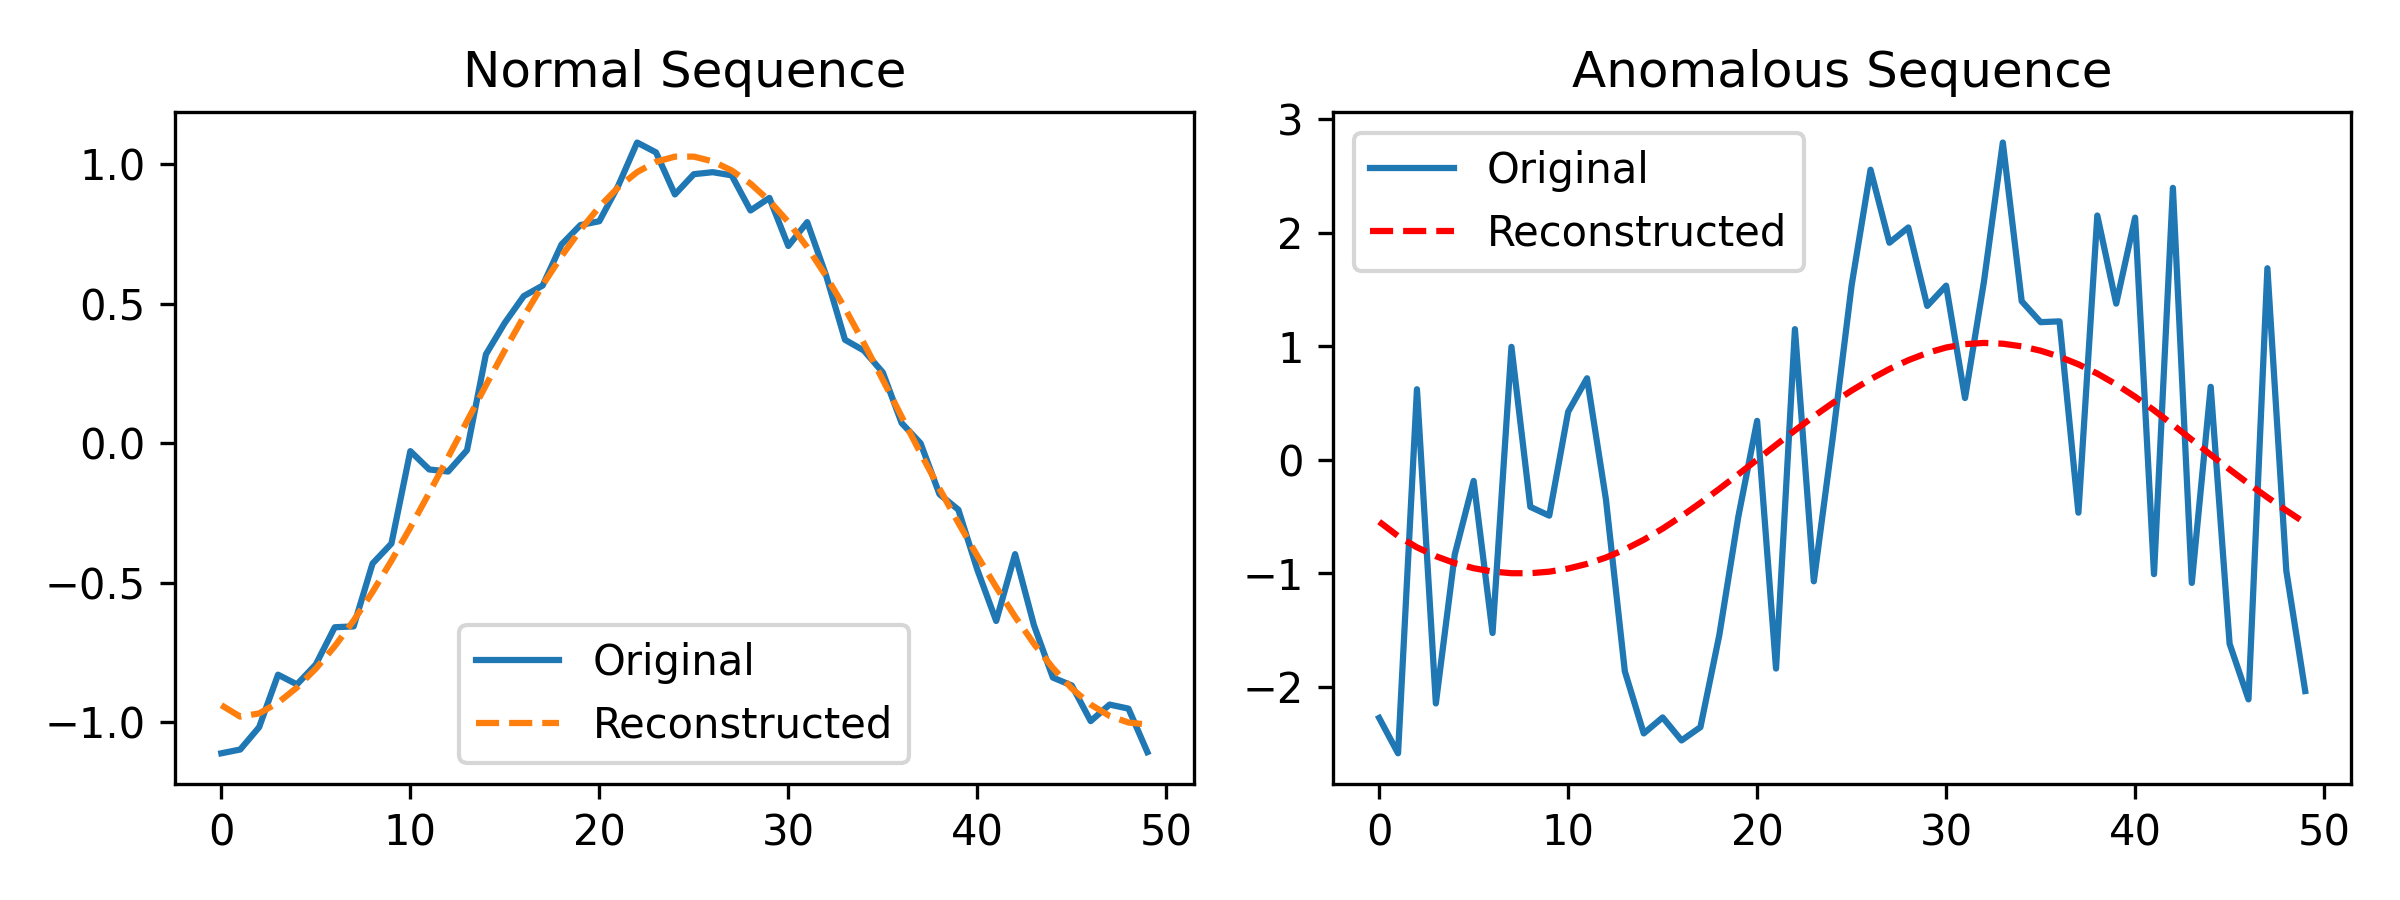
\includegraphics[width=0.9\textwidth]{images/lstm_anomaly_detection.png}
    \caption{Example of normal (left) and anomalous (right) sequences. Dashed lines represent reconstructed sequences.}
    \label{fig:anomaly_detection}
\end{figure}

{\bf Visualizing Detected Anomalies.} 
We randomly sample 12 sequences from the test set, classify them, and color them accordingly—blue for normal and red for anomalies.

\begin{figure}[ht!]
    \centering
    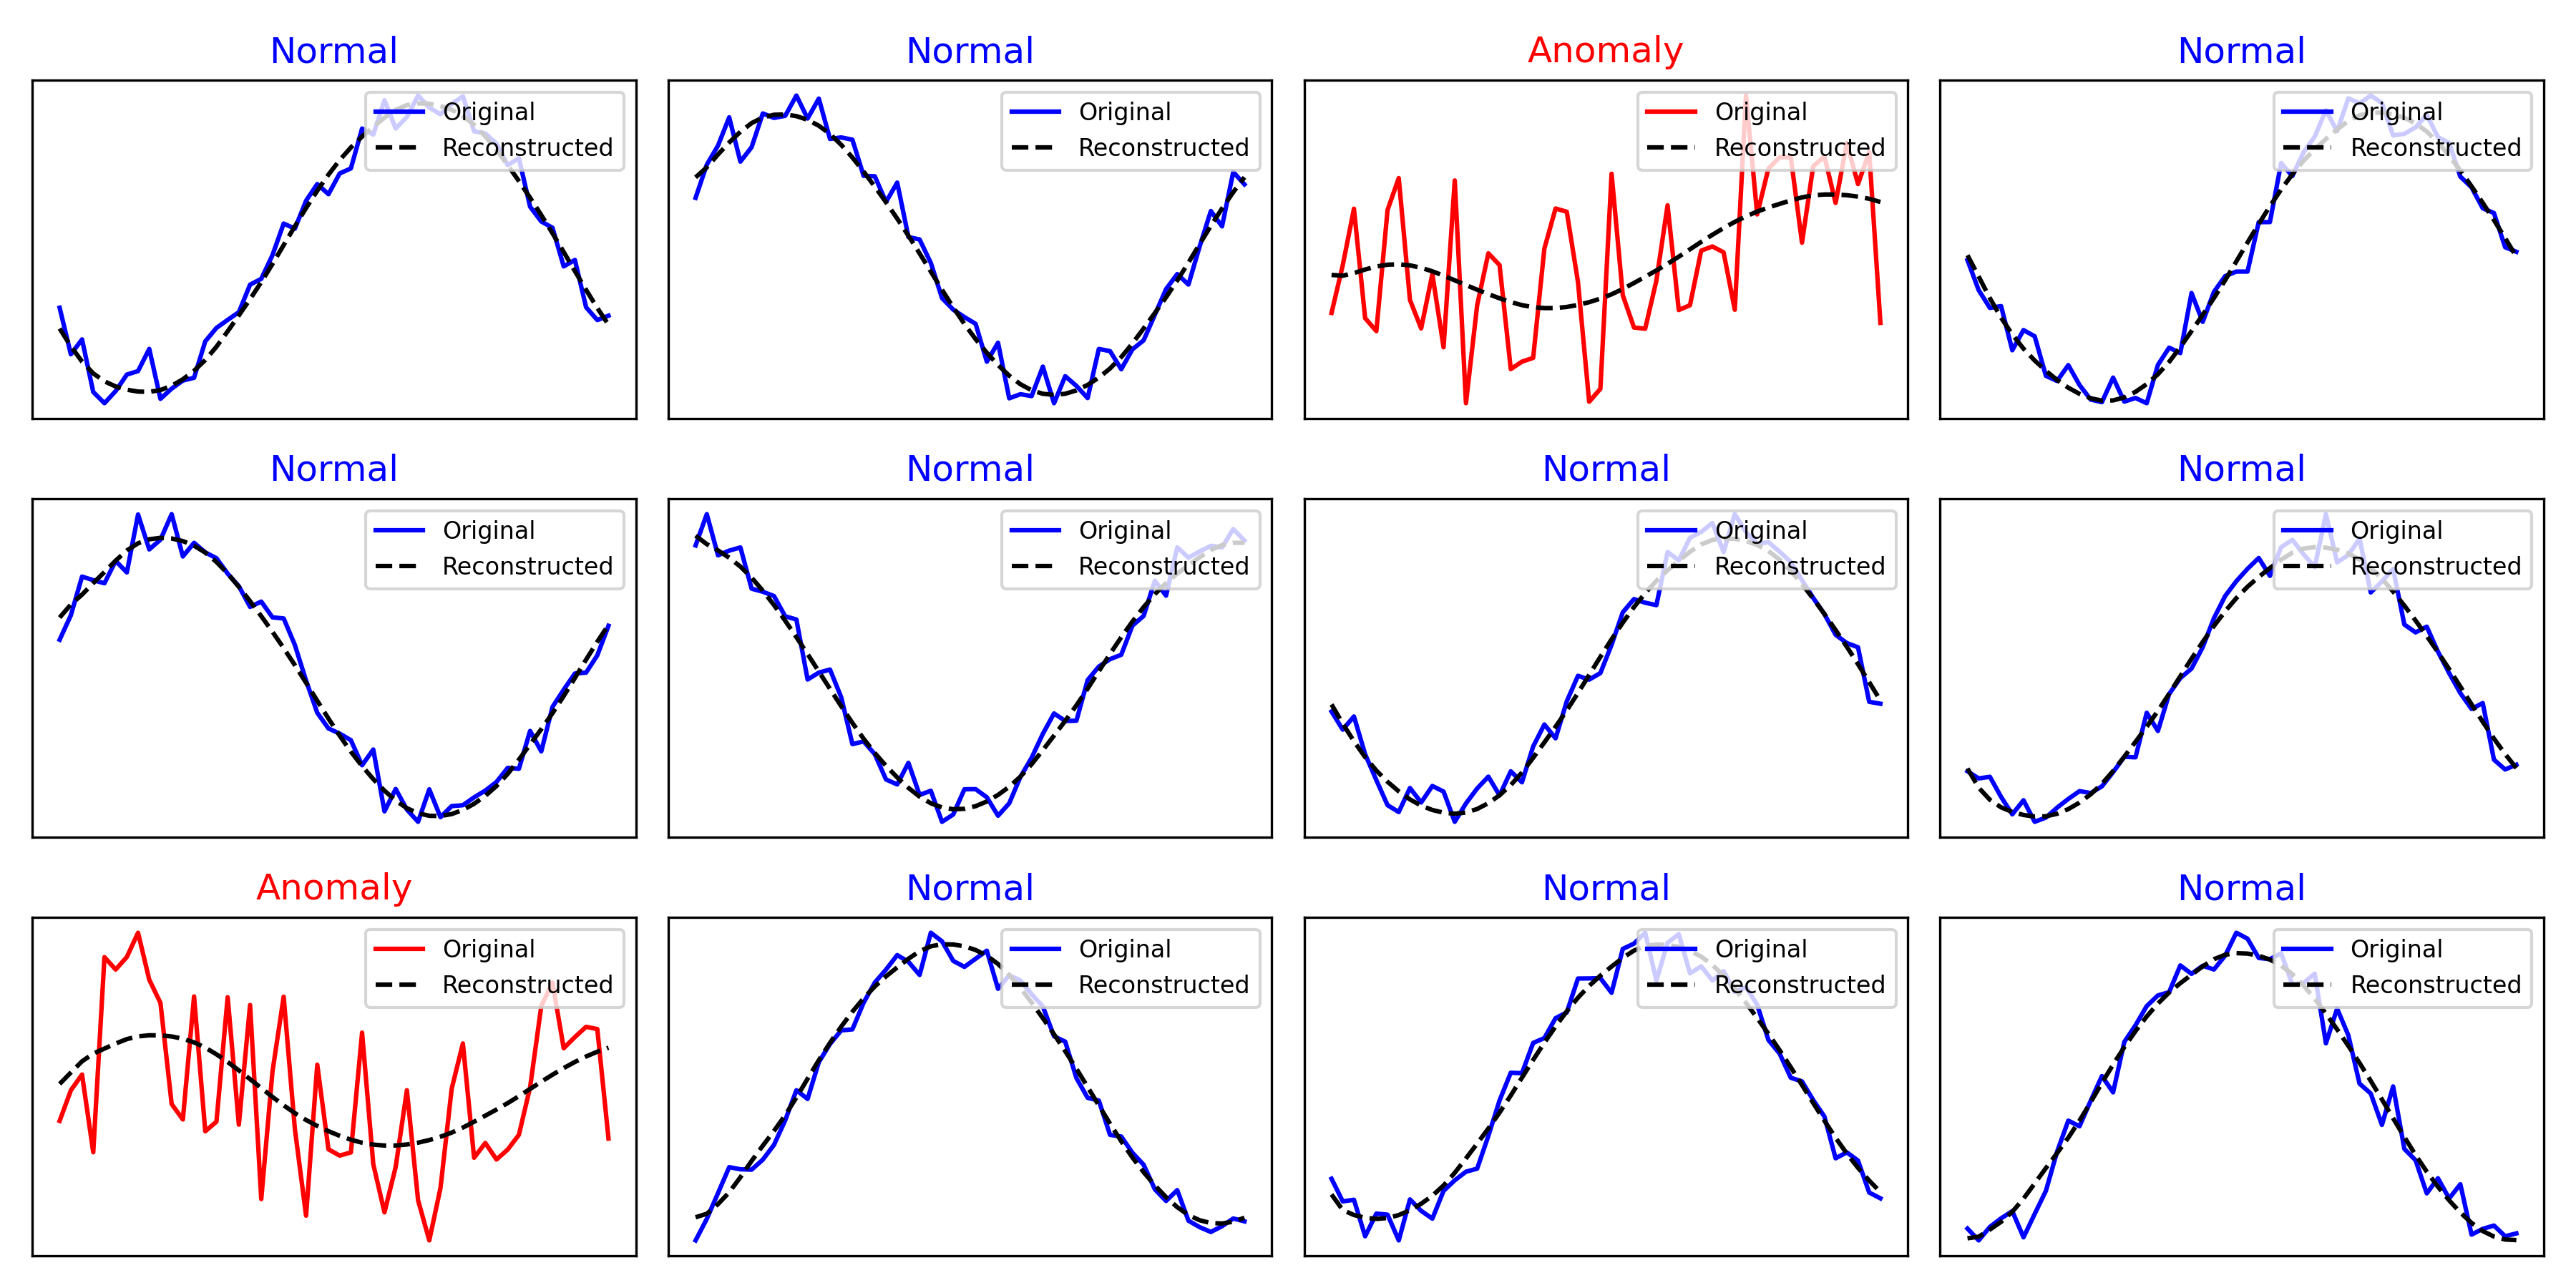
\includegraphics[width=0.9\textwidth]{images/lstm_anomaly_detection_samples_selected.png}
    \caption{Illustration of the detection and correction of the sensor anomaly.}
    \label{fig:training_loss}
\end{figure}


\begin{codeonly}{Visualizing Anomalies}
import matplotlib.pyplot as plt

# Select 12 random test samples
num_samples = 12
indices = np.random.choice(len(X_test), num_samples, replace=False)

# Compute reconstruction errors
model.eval()
with torch.no_grad():
    X_reconstructed = model(X_test.to(device))

reconstruction_errors = torch.mean((X_test - X_reconstructed) ** 2, dim=(1, 2)).cpu().numpy()

# Detect anomalies based on threshold
threshold = np.percentile(reconstruction_errors, 90)
y_pred = (reconstruction_errors > threshold).astype(int)  # 1 = Anomaly, 0 = Normal

# Plot the selected samples
plt.figure(figsize=(12, 6))
for i, idx in enumerate(indices):
    color = 'red' if y_pred[idx] == 1 else 'blue'
    
    plt.subplot(3, 4, i + 1)
    plt.plot(X_test[idx].cpu().numpy(), color=color, label="Original")
    plt.plot(X_reconstructed[idx].cpu().numpy(), linestyle="dashed", color="black", label="Reconstructed")
    plt.title(f"{'Anomaly' if y_pred[idx] == 1 else 'Normal'}", color=color)
    plt.xticks([]), plt.yticks([])
    plt.legend(fontsize=8, loc="upper right")

plt.tight_layout()
plt.savefig("lstm_anomaly_detection_samples_selected.png", dpi=300)
plt.show()
\end{codeonly}

\begin{recommendationbox}
There are quite different architectures of neural networks. The connectivity is a crucial choice for the functionality of the network. But also training datasets and optimisation strategies determine the success or failure of the network functionality and quality. 
\end{recommendationbox}

\begin{recommendationbox}
There is not one good or bad network or architecture, but different approaches are good for different applications. 
\end{recommendationbox}
 % 

\chapter{Large Language Models}

\section{LLM Network as Sequence-to-Sequence Machines via Transformer Models}

At their core, Large Language Models (LLMs) are sequence-to-sequence machines that generate a response sequence given an input sequence of words, converted into tokens. However, the way they process and generate these sequences involves several layers of complexity:

\begin{enumerate}
    \item \textbf{Contextual Understanding via Self-Attention} \\
    Unlike simple sequence models (e.g., RNNs), Transformers use self-attention to consider all tokens in a sequence simultaneously. This allows them to capture dependencies across long contexts.

    \item \textbf{Probability-Based Token Generation} \\
    At each step, the model predicts the next token by computing a probability distribution over the vocabulary. The output sequence is formed by sampling or selecting the most probable token at each step.

    \item \textbf{Task-Specific Adaptations}
    \begin{itemize}
        \item \textbf{Text Generation} (GPT, LLaMA, Mistral): Autoregressive models predict one token at a time, conditioning each step on previous outputs.
        \item \textbf{Text Understanding} (BERT): Masked language models predict missing tokens given bidirectional context.
        \item \textbf{Instruction-Tuned Models} (ChatGPT, Claude): Fine-tuned on dialogue and instruction-following data, allowing multi-turn interactions.
    \end{itemize}
\end{enumerate}

So, while LLMs fundamentally map an input sequence to an output sequence, their real power comes from how they encode context, manage dependencies, and adapt to various tasks through fine-tuning and prompting.

Large Language Models (LLMs) have revolutionized natural language processing (NLP) through the use of Transformer architectures. Introduced by Vaswani et al. in 2017, Transformers have surpassed previous recurrent and convolutional models in both efficiency and scalability. Let us give a quick overview of Transformer architectures and their role in modern LLMs.

The Transformer model is based on the self-attention mechanism and is composed of an encoder-decoder structure. However, most LLMs, such as GPT and BERT, utilize only the encoder or decoder portion.

%------------------------------------------------------------------------------
%
%------------------------------------------------------------------------------

{\bf Self-attention} processes an input sequence of \( n \) tokens, where each token represents a word or subword from a given text. The input is converted into a numerical representation in three steps.

First, the input sentence is tokenized using a tokenizer such as WordPiece or Byte-Pair Encoding. For example, the sentence:

\[
\mytext{"write code for problem a"}
\]

is split into the tokens:

\[
\{\mytext{write}, \mytext{code}, \mytext{for}, \mytext{problem}, \mytext{a}\}
\]

resulting in \( n = 5 \) tokens.

Each token is then mapped to a high-dimensional vector using a learned embedding matrix \( E \in \mathbb{R}^{V \times d_{\text{model}}} \), where:
- \( V \) is the vocabulary size.
- \( d_{\text{model}} \) is the embedding dimension.

The input sequence is represented as a matrix:

\[
X = \left( \begin{array}{c} x_1 \\ x_2 \\ \vdots \\ x_n \end{array}\right) \in \mathbb{R}^{n \times d_{\text{model}}},
\]

where each row \( x_i \in \mathbb{R}^{1 \times d_{\text{model}}} \) corresponds to the embedding of a token.

\textbf{Positional Encoding:} Since Transformers lack an inherent sequence structure, a {\bf positional encoding matrix} \( P \in \mathbb{R}^{n \times d_{\text{model}}} \) is added:

\[
X_{\text{final}} = X + P,
\]

where: \( P \) is a matrix containing position-specific values that help encode the order of tokens and each row \( P_i \in \mathbb{R}^{1 \times d_{\text{model}}} \) corresponds to the positional encoding for the \( i \)-th token.
The positional encoding matrix \( P \in \mathbb{R}^{n \times d_{\text{model}}} \) is defined using sinusoidal functions, where each element is computed as 
\[
P_{(i, 2j)} = \sin\left(\frac{i}{10000^{2j/d_{\text{model}}}}\right), \quad P_{(i, 2j+1)} = \cos\left(\frac{i}{10000^{2j/d_{\text{model}}}}\right),
\]
with \( i \) representing the token position and \( j \) the dimension index. The resulting matrix \( X_{\text{final}} \) is then passed to the self-attention mechanism, where each token can attend to all others. This allows the model to differentiate between identical words appearing in different positions within the sequence. The resulting matrix \( X_{\text{final}} \) is the input to the self-attention mechanism, where each token can attend to all others.
    
This processed matrix \( X_{\text{final}} \) serves as the input to the self-attention mechanism, where each token can attend to all other tokens in the sequence. For each token, three matrices project its embedding into three key representations:
\begin{itemize}
    \item \textbf{Query matrix} \( Q \in \mathbb{R}^{n \times d_k} \) 
    \item \textbf{Key matrix} \( K \in \mathbb{R}^{n \times d_k} \) 
    \item \textbf{Value matrix} \( M \in \mathbb{R}^{n \times d_v} \) 
\end{itemize}
These matrices are obtained from the input embedding matrix \( X \in \mathbb{R}^{n \times d_{\text{model}}} \) through learned weight matrices \( W^Q \), \( W^K \), and \( W^M \):

\begin{equation}
    Q = X W^Q, \quad K = X W^K, \quad M = X W^M,
\end{equation}
where \( W^Q, W^K \in \mathbb{R}^{d_{\text{model}} \times d_k} \) and \( W^M \in \mathbb{R}^{d_{\text{model}} \times d_v} \) are learnable parameter matrices.

The attention scores are computed using the scaled dot-product attention:

\begin{equation}
    \text{Attention}(Q, K, M) = \text{softmax} \left( \frac{Q K^T}{\sqrt{d_k}} \right) M.
\end{equation}
The softmax function is applied to each row of a matrix \( S \in \mathbb{R}^{n \times n} \), where each element is transformed as:

\[
\operatorname{softmax}(S)_{ij} = \frac{\exp(S_{ij})}{\sum_{k=1}^{n} \exp(S_{ik})}.
\]

This ensures that for each row \( i \), the values satisfy:

\[
\sum_{j=1}^{n} \operatorname{softmax}(S)_{ij} = 1,
\]

converting the attention scores into a probability distribution across all tokens. Since \( Q \in \mathbb{R}^{n \times d_k} \) and \( K^T \in \mathbb{R}^{d_k \times n} \), the matrix product \( Q K^T \) results in an attention score matrix of shape \( \mathbb{R}^{n \times n} \). After applying the softmax function row-wise, the resulting matrix is multiplied by \( V \in \mathbb{R}^{n \times d_v} \), producing the final output
\[
\operatorname{Attention}(Q, K, M) \in \mathbb{R}^{n \times d_v}.
\]
We summarize:
\begin{itemize}
    \item \( Q K^T \in \mathbb{R}^{n \times n} \) computes similarity scores between all tokens.
    \item The scaling factor \( \sqrt{d_k} \) prevents large values inside the softmax function.
    \item The softmax function normalizes the similarity scores.
\end{itemize}

\textbf{Multi-Head Attention:} Instead of using a single attention mechanism, Transformers employ multiple attention heads to capture different aspects of the input. Given an input sequence \( X \in \mathbb{R}^{n \times d_{\text{model}}} \), multiple projections of \( Q, K, M \) are computed for each attention head. Each head with index \( i \) applies self-attention independently using separate weight matrices:
\begin{equation}
    Q_i = X W^Q_i, \quad K_i = X W^K_i, \quad M_i = X W^M_i,
\end{equation}
where
\[
W^Q_i, W^K_i \in \mathbb{R}^{d_{\text{model}} \times d_k}, \quad W^M_i \in \mathbb{R}^{d_{\text{model}} \times d_v}
\]
are learnable weight matrices for each head. Self-attention is then computed for each head as:
\begin{equation}
    \operatorname{head}_i = \operatorname{Attention}(Q_i, K_i, M_i),
\end{equation}
with \( \operatorname{head}_i \in \mathbb{R}^{n \times d_v} \). The outputs of all \( h \) heads are then concatenated:
\begin{equation}
    \operatorname{MultiHead}(Q, K, M) = \operatorname{Concat}(\operatorname{head}_1, \dots, \operatorname{head}_h) W^O,
\end{equation}
where \( W^O \in \mathbb{R}^{h d_v \times d_{\text{model}}} \) is a learned projection matrix that maps the concatenated outputs back to the model's hidden dimension \( d_{\text{model}} \). The final output has the shape:

\[
\operatorname{MultiHead}(Q, K, M) \in \mathbb{R}^{n \times d_{\text{model}}}.
\]

%------------------------------------------------------------------------------
%
%------------------------------------------------------------------------------
{\bf Loss Function for Attention:} The self-attention mechanism is trained by minimizing a loss function that measures the discrepancy between the model's predictions and the target outputs. Given an input sequence \( X \) and corresponding ground truth output \( Y \), the model produces an output representation \( Z \) from self-attention:

\[
Z = \operatorname{Attention}(Q, K, M) = \operatorname{softmax} \left( \frac{Q K^T}{\sqrt{d_k}} \right) M.
\]

For multi-head attention, the output is:
\[
Z = \operatorname{MultiHead}(Q, K, M) = \operatorname{Concat}(\operatorname{head}_1, \dots, \operatorname{head}_h) W^O.
\]
In a sequence-to-sequence task, such as machine translation, the model processes an input sequence and generates an output sequence token by token. The loss function measures how well the predicted probability distribution over the vocabulary matches the ground truth sequence.

%------------------------------------------------------------------------------
%
%------------------------------------------------------------------------------
{\bf Output Projection to Vocabulary:} Since the output of self-attention and multi-head attention is a sequence representation matrix \( Z \in \mathbb{R}^{n \times d_{\text{model}}} \), it must be mapped to a probability distribution over the vocabulary. This is done using a learned output weight matrix \( W_{\text{out}} \in \mathbb{R}^{d_{\text{model}} \times V} \) and a bias term \( b_{\text{out}} \in \mathbb{R}^{V} \), where \( V \) is the vocabulary size. The transformation is performed as follows:
\[
Z_{\text{logits}} = Z W_{\text{out}} + b_{\text{out}},
\]
resulting in \( Z_{\text{logits}} \in \mathbb{R}^{n \times V} \), where each row represents a raw score (logit) over all possible vocabulary words for the corresponding input token.

{\bf Converting Logits to Probabilities:} Since \( Z_{\text{logits}} \) contains unnormalized scores, we apply the softmax function row-wise to obtain a valid probability distribution:
\[
Z_{\text{pred}} = \operatorname{softmax}(Z_{\text{logits}}),
\]
where \( Z_{\text{pred}} \in \mathbb{R}^{n \times V} \) and each row is a probability distribution over the vocabulary, summing to 1.

{\bf Comparison with Ground Truth:} Given a sequence of true output tokens \( Y = (y_1, y_2, ..., y_n) \), where each \( y_t \) is an integer index in the vocabulary, we define the corresponding one-hot encoded matrix:
\[
Z_Y \in \mathbb{R}^{n \times V}, 
\]
where each row \( Z_{Y,t} \) is a one-hot vector (in mathematical terms a unity vector $e_{i_t}$ with position $i_t$ for the word in the vocabulary) indicating the correct token at position \( t \). Since \( Z_Y \) is one-hot, we extract the predicted probability assigned to the correct token \( i_t \) at each position \( t \):
\[
P_t = Z_{\text{pred}, t, i_t}.
\]

%------------------------------------------------------------------------------
%
%------------------------------------------------------------------------------
{\bf Cross-Entropy Loss:} The loss function measures the model’s ability to assign high probability to the correct next token. It is computed as:
\[
\mathcal{L} = - \sum_{t=1}^{n} \log P_t, 
\]
where we note that $P_t$ is between $0$ and $1$, such that larger $P_t$ corresponds to lower $\mathcal{L}$. This ensures that if the model assigns low probability to the correct token, the loss is high, guiding the optimization process to improve predictions.

{\bf Training with Gradient Descent:} The loss gradients are computed with respect to all learnable parameters, including the attention weight matrices and the output projection:
\[
\frac{\partial \mathcal{L}}{\partial W^Q}, \quad \frac{\partial \mathcal{L}}{\partial W^K}, \quad \frac{\partial \mathcal{L}}{\partial W^V}, \quad \frac{\partial \mathcal{L}}{\partial W^O}, \quad \frac{\partial \mathcal{L}}{\partial W_{\text{out}}}.
\]
The parameters are updated using gradient-based optimization methods such as Adam:
\[
W^Q \leftarrow W^Q - \eta \frac{\partial \mathcal{L}}{\partial W^Q}, \quad W^K \leftarrow W^K - \eta \frac{\partial \mathcal{L}}{\partial W^K}, \quad W^V \leftarrow W^V - \eta \frac{\partial \mathcal{L}}{\partial W^V}, \quad W_{\text{out}} \leftarrow W_{\text{out}} - \eta \frac{\partial \mathcal{L}}{\partial W_{\text{out}}}.
\]
where \( \eta \) is the learning rate. The optimization process is repeated for multiple input-output pairs to gradually improve the model's predictions. 

%------------------------------------------------------------------------------
%
%------------------------------------------------------------------------------
Popular LLMs include:
\begin{itemize}
    \item \textbf{BERT} (Bidirectional Encoder Representations from Transformers) - Uses the encoder stack for contextual embeddings.
    \item \textbf{GPT} (Generative Pretrained Transformer) - Uses the decoder stack for autoregressive text generation.
    \item \textbf{T5} (Text-to-Text Transfer Transformer) - Converts all NLP tasks into a text-to-text format.
\end{itemize}

%==============================================================================
%
%==============================================================================
\section{Implementing and Training a Simple Transformer-Based LLM}

In the previous section, we explored the fundamental concepts behind self-attention, multi-head attention, and how transformers process sequences. We now implement a simple transformer-based language model (LLM) in PyTorch to demonstrate these principles in practice.

Transformers process input sequences by first embedding tokens into high-dimensional vectors and then refining these representations through multiple layers of self-attention and feedforward transformations. The model is trained to predict the next token in a sequence, adjusting its parameters using gradient descent.

This section provides a practical walkthrough of implementing a transformer-based LLM, covering:
\begin{itemize}
    \item The core components of a transformer, including positional encoding and self-attention.
    \item The forward pass of a transformer model applied to text.
    \item Training the model on a small dataset.
    \item Using the trained model to generate text.
\end{itemize}

We begin by defining a simple transformer model using PyTorch, followed by data preprocessing, training, and text generation.


\begin{codeonly}{Simple Transformer for Text Processing}
import torch
import torch.nn as nn
import math

# Define the Positional Encoding
class PositionalEncoding(nn.Module):
    def __init__(self, d_model, max_len=5000):
        super(PositionalEncoding, self).__init__()
        pe = torch.zeros(max_len, d_model)
        position = torch.arange(0, max_len, dtype=torch.float).unsqueeze(1)
        div_term = torch.exp(torch.arange(0, d_model, 2).float() * (-math.log(10000.0) / d_model))
        pe[:, 0::2] = torch.sin(position * div_term)
        pe[:, 1::2] = torch.cos(position * div_term)
        pe = pe.unsqueeze(0).transpose(0, 1)
        self.register_buffer('pe', pe)

    def forward(self, x):
        return x + self.pe[:x.size(0), :]

# Define the Transformer Block
class TransformerBlock(nn.Module):
    def __init__(self, d_model, num_heads, d_ff):
        super(TransformerBlock, self).__init__()
        self.attention = nn.MultiheadAttention(d_model, num_heads)
        self.norm1 = nn.LayerNorm(d_model)
        self.norm2 = nn.LayerNorm(d_model)
        self.ff = nn.Sequential(
            nn.Linear(d_model, d_ff),
            nn.ReLU(),
            nn.Linear(d_ff, d_model)
        )

    def forward(self, x):
        attn_out, _ = self.attention(x, x, x)
        x = self.norm1(x + attn_out)
        x = self.norm2(x + self.ff(x))
        return x

# Define the Transformer Model
class SimpleTransformer(nn.Module):
    def __init__(self, d_model, num_heads, num_layers, vocab_size, max_len, d_ff=2048):
        super(SimpleTransformer, self).__init__()
        self.embedding = nn.Embedding(vocab_size, d_model)
        self.positional_encoding = PositionalEncoding(d_model, max_len)
        self.layers = nn.ModuleList([TransformerBlock(d_model, num_heads, d_ff) for _ in range(num_layers)])
        self.fc_out = nn.Linear(d_model, vocab_size)

    def forward(self, x):
        x = self.embedding(x)
        x = self.positional_encoding(x)
        for layer in self.layers:
            x = layer(x)
        return self.fc_out(x)

# Example usage
model = SimpleTransformer(d_model=32, num_heads=2, num_layers=2, vocab_size=56, max_len=6)
print(model)
\end{codeonly}

\subsection{Setting Up, Training, and Using Our Simple LLM}
To train and use our simple transformer-based LLM, we will:
1. Define a small vocabulary and dataset
2. Preprocess the data
3. Train the model
4. Generate text using the trained model

\subsubsection{Defining a Small Vocabulary and Dataset}
We use a simple vocabulary with a set of basic sentences for training.

\begin{codeonly}{Define Vocabulary and Dataset}
vocab = {1: "I", 2: "am", 3: "hungry", ..., 55: "was"}
sentences = [
    "I am hungry",
    "you are tired",
    "we are happy",
    "they are sad",
    "it is simple",
    "the weather is nice",
]
\end{codeonly}

\subsubsection{Preprocessing Data}
Tokenizing and padding sentences for training.

\begin{codeonly}{Tokenization and Padding}
def tokenize_sentence(sentence, vocab):
    return [key for word in sentence.split() for key, value in vocab.items() if value == word]

def pad_sequence(seq, max_len, pad_value=0):
    return seq + [pad_value] * (max_len - len(seq)) if len(seq) < max_len else seq[:max_len]
\end{codeonly}

\subsubsection{Training the Model}
Now, we train the transformer model using a simple training loop.

\begin{codeonly}{Train the Transformer}
import torch.optim as optim

model = SimpleTransformer(d_model=32, num_heads=2, num_layers=2, vocab_size=56, max_len=6)
criterion = nn.CrossEntropyLoss(ignore_index=0)
optimizer = optim.Adam(model.parameters(), lr=0.001)

def train(model, dataloader, epochs=101):
    model.train()
    for epoch in range(epochs):
        total_loss = 0
        for x, y in dataloader:
            optimizer.zero_grad()
            output = model(x)
            loss = criterion(output.view(-1, 56), y.view(-1))
            loss.backward()
            optimizer.step()
            total_loss += loss.item()
        if epoch % 100 == 0:
            print(f"Epoch {epoch+1}, Loss: {total_loss/len(dataloader):.4f}")
train(model, dataloader)
\end{codeonly}

\subsubsection{Generating Text with the Trained Model}
We generate sentences by feeding input sequences into the trained model.

\begin{codeonly}{Generate Text}
def generate_text(model, seed_seq, max_length=6):
    model.eval()
    with torch.no_grad():
        seq = seed_seq.clone()
        for _ in range(max_length - len(seq)):
            output = model(seq.unsqueeze(0))
            next_token = torch.argmax(output[:, -1, :], dim=-1)
            seq = torch.cat([seq, next_token], dim=0)
    return seq

# Example generation
seed = torch.tensor([1, 2])  # "I am"
output_seq = generate_text(model, seed)
print("Generated Sequence:", output_seq.tolist())
\end{codeonly}

This section provides a fundamental workflow for setting up, training, and using a simple transformer-based LLM.

To train a large-scale language model (LLM), the process extends beyond a simple dataset and model architecture. Large LLMs require vast amounts of text data, often consisting of terabytes of diverse sources such as books, articles, and web content. Instead of training on small, manually defined vocabularies, modern LLMs utilize subword tokenization techniques, such as SentencePiece or Byte-Pair Encoding (BPE), to handle open-ended vocabulary sizes efficiently. 

The model itself is composed of billions of parameters, requiring parallelized training across multiple GPUs or TPUs using techniques such as model parallelism and pipeline parallelism. The optimization process involves advanced gradient accumulation, mixed-precision training for efficiency, and adaptive optimizers like AdamW. 

Additionally, large-scale training requires extensive pretraining followed by task-specific fine-tuning, ensuring both general language understanding and domain-specific capabilities. Due to the computational scale, training an LLM can take weeks or months on dedicated high-performance clusters.

Training large-scale language models (LLMs) requires immense computational resources, typically measured in GPU hours. For example, 
\begin{itemize}
\item
GPT-3 (175 billion parameters) was trained on approximately 3640 petaflop-days, which translates to roughly 10 million GPU hours on NVIDIA V100 GPUs. 
\item
More recent models, such as GPT-4 and PaLM-2, likely required even higher computational budgets, often exceeding 20–30 million GPU hours. 
\end{itemize}
In contrast, a high-performance supercomputer like HOREKA at KIT, which features NVIDIA A100 GPUs, delivers a peak performance of around 17 petaflops for AI workloads. Assuming an efficient utilization of HOREKA’s full AI capacity, training a model like GPT-3 would take several months, whereas dedicated large-scale clusters, such as those used by OpenAI or Google, can parallelize the workload across thousands of GPUs, reducing training time to a few weeks. This illustrates the sheer scale of computational power needed for modern LLM training compared to even high-end academic supercomputers.

\begin{recommendationbox}
Training a LLM to achieve very high quality is a major task, which needs a lot of resources both in terms of preparation as well as computing power. However, this effort is invested today by a growing number of actors on an international scale. Using and finetuning models is already very easy and will become more feasible, with LLM functionality becoming ubiquitous already now. Focus on modularly leveraging the growing potential of LLM intelligence combining it with your applications and services. 
\end{recommendationbox}


%==============================================================================
%
%==============================================================================
\section{Install Your Own LLM, Chat with it and Develop Applications}

Several open-source frameworks allow users to install and run large language models (LLMs) on local machines or servers without requiring proprietary cloud-based solutions. 
\begin{itemize}
\item
One of the most user-friendly tools is {\tt Ollama}, which provides a streamlined interface for running optimized LLMs on consumer hardware with GPU acceleration. 
\item
Other notable frameworks include {\tt LM Studio}, which offers a graphical interface for managing local LLMs, and {\tt Text Generation WebUI}, which provides an interactive web-based interface for experimenting with different models. 
\item
Additionally, {\tt GPTQ-for-LLaMa} and {\tt AutoGPTQ} support quantized models for memory-efficient execution. For more advanced setups, {\tt vLLM} enables high-throughput inference, while {\tt llama.cpp} provides a highly optimized C++ implementation of LLaMA models for running on CPU-based systems. These frameworks allow researchers and developers to experiment with LLMs without requiring access to large-scale cloud infrastructure.
\item
One of the most widely used open-source frameworks for installing and running large language models (LLMs) is the {\tt Hugging Face Transformers} library. It provides pre-trained models, easy-to-use APIs, and support for fine-tuning on custom datasets. The library includes models such as GPT, BERT, T5, and LLaMA, among many others, and integrates seamlessly with PyTorch, TensorFlow, and JAX. Hugging Face also offers {\tt Optimum} for hardware optimizations, allowing efficient execution on GPUs and specialized accelerators such as TensorRT and Habana Gaudi. Combined with {\tt datasets} and {\tt accelerate}, it enables large-scale training and inference on local or distributed systems. While Hugging Face primarily focuses on cloud and research environments, it can also be used locally with models optimized for consumer hardware, making it a versatile choice for both academic and production applications.
\end{itemize}

Ollama is a framework that allows users to run local LLMs efficiently. To install Ollama and run a model locally, follow these steps:

{\bf Downloading and Installing Ollama}  
To install Ollama, download and execute the official installation script:

\begin{codeonly}{Install Ollama}
curl -fsSL https://ollama.com/install.sh | sh
\end{codeonly}

{\bf Verifying the Installation}  
After installation, check if Ollama is installed correctly by running:

\begin{codeonly}{Check Ollama Version}
ollama --version
\end{codeonly}

This command should return the installed version of Ollama.

{\bf Pulling and Running a Pre-Trained Model}  
To download and execute a pre-trained model, such as Mistral, use:

\begin{codeonly}{Download and Run Mistral}
ollama pull mistral
ollama run mistral
\end{codeonly}

The first command downloads the model, while the second runs it locally.


{\bf Starting and Stopping the Ollama Server}  
Ollama can run as a background service to manage models efficiently. To start the Ollama server, use:

\begin{codeonly}{Start the Ollama Server}
ollama serve
\end{codeonly}

This command launches the Ollama server, making it ready to handle model requests.

To stop the running Ollama server, use:

\begin{codeonly}{Stop the Ollama Server}
ollama stop
\end{codeonly}

This will gracefully shut down the Ollama service.

{\bf Listing Available Models}  
To check which models are installed locally and available for use, run:

\begin{codeonly}{List Installed Models}
ollama list
\end{codeonly}

This command outputs a list of all locally stored models, along with their sizes and versions.

%==============================================================================
%   
%==============================================================================
\subsection{Interacting with Ollama's Local API}

Ollama runs a local REST API on `http://localhost:11434`, allowing interaction with models using HTTP requests. The following examples demonstrate how to generate text using the API with `curl` and Python.

\subsubsection{Using Curl}

\subsubsection{Description}

The following `curl` command sends a request to the Ollama API, asking it to generate text based on a given prompt.

\begin{codeonly}{Using Curl}
curl -X POST http://localhost:11434/api/generate \
-H "Content-Type: application/json" \
-d '{
  "model": "mistral",
  "prompt": "What is the capital of Germany?",
  "stream": false
}'
\end{codeonly}

\subsubsection{Using Python}

Alternatively, you can use Python’s `requests` library to send the same request programmatically.

\begin{codeonly}{Using Python}
import requests
import json

url = "http://localhost:11434/api/generate"
data = {
    "model": "mistral",
    "prompt": "What is the capital of Germany?",
    "stream": False
}

response = requests.post(url, json=data)
print(response.json())
\end{codeonly}


\subsubsection{Using Ollama's Python API}

Ollama provides a python API to interact with its local server. 

\begin{codeonly}{Using Ollama's Python API}
import ollama

# Load a local model
model = 'mistral'

# Generate a response
response = ollama.chat(model=model, messages=[{"role": "user", "content": "What is the capital of France?"}])

# Print the response
print(response['message']['content'])
\end{codeonly}


%==============================================================================
%   
%==============================================================================
\subsection{A Local UI with Personal History for Ollama}
To create a simple local UI with personal chat history for Ollama, we can use Flask. Below is an example of how to build such a system. You need to use pip to install \texttt{flask} before this can work. 

\begin{codeonly}{Flask-Based Local Chat UI}
from flask import Flask, request, jsonify, render_template
import ollama

app = Flask(__name__)

chat_history = []  # Stores full chat history

@app.route('/')
def index():
    return render_template('index.html')  # Serves the HTML UI

@app.route('/chat', methods=['POST'])
def chat():
    user_input = request.json.get('message')

    if not user_input:
        return jsonify({'error': 'No message provided'}), 400

    # Append current message to chat history
    chat_history.append({"role": "user", "content": user_input})

    # Send full conversation history to Ollama
    response = ollama.chat(model="deepseek-r1:7b", messages=chat_history)

    # Extract Ollama's response
    bot_reply = response['message']['content']

    # Append bot response to chat history
    chat_history.append({"role": "assistant", "content": bot_reply})

    return jsonify({'response': bot_reply, 'history': chat_history})

if __name__ == '__main__':
    app.run(debug=True)
\end{codeonly}

This simple Flask app allows users to interact with an LLM locally while maintaining chat history.
We saved this as \texttt{ollama\_flask\_server.py} in the doce subdirectory \texttt{ollama\_UI}. Also, we provide the file \texttt{index.html} in the subdirectory \texttt{templates} to control the UI. 


\subsubsection{Installing Dependencies}

Before running the server, you need to install Flask. You can do this using pip:

\begin{codeonly}{Installing Flask}
pip install flask
\end{codeonly}

Ensure that you also have Ollama installed and running locally.

\subsubsection{Setting Up the UI}

The HTML file that provides the user interface should be saved as \texttt{index.html} in the \texttt{templates} subdirectory inside \texttt{code06}. Below is the content of this file:

\begin{codeonly}{index.html}
<!DOCTYPE html>
<html lang="en">
<head>
    <meta charset="UTF-8">
    <meta name="viewport" content="width=device-width, initial-scale=1.0">
    <title>Chatbot</title>
    <style>
        body {
            font-family: Arial, sans-serif;
            margin: 0;
            padding: 20px;
            background-color: #f4f4f4;
        }
        #chat-container {
            width: 50%;
            max-width: 600px;
            margin: auto;
            background: white;
            padding: 20px;
            border-radius: 10px;
            box-shadow: 0px 0px 10px rgba(0, 0, 0, 0.1);
        }
        #chat-box {
            height: 300px;
            overflow-y: auto;
            border: 1px solid #ddd;
            padding: 10px;
            margin-bottom: 10px;
            background: #fff;
        }
        .message {
            padding: 8px;
            margin: 5px 0;
            border-radius: 5px;
        }
        .user { background: #d1e7fd; text-align: right; }
        .bot { background: #e6e6e6; text-align: left; }
        input, button {
            width: 100%;
            padding: 10px;
            margin-top: 10px;
            border: none;
            border-radius: 5px;
        }
        button {
            background: #007bff;
            color: white;
            cursor: pointer;
        }
        button:hover {
            background: #0056b3;
        }
    </style>
</head>
<body>

    <div id="chat-container">
        <h2>Chatbot</h2>
        <div id="chat-box"></div>
        <input type="text" id="user-input" placeholder="Type a message..." onkeypress="handleKeyPress(event)">
        <button onclick="sendMessage()">Send</button>
    </div>

    <script>
        function sendMessage() {
            let userInput = document.getElementById("user-input").value;
            if (userInput.trim() === "") return;

            let chatBox = document.getElementById("chat-box");

            // Append user message
            let userMessage = document.createElement("div");
            userMessage.classList.add("message", "user");
            userMessage.textContent = userInput;
            chatBox.appendChild(userMessage);

            document.getElementById("user-input").value = ""; // Clear input
            chatBox.scrollTop = chatBox.scrollHeight; // Auto-scroll

            // Send request to Flask server
            fetch("/chat", {
                method: "POST",
                headers: { "Content-Type": "application/json" },
                body: JSON.stringify({ message: userInput })
            })
            .then(response => response.json())
            .then(data => {
                let botMessage = document.createElement("div");
                botMessage.classList.add("message", "bot");
                botMessage.textContent = data.response;
                chatBox.appendChild(botMessage);
                chatBox.scrollTop = chatBox.scrollHeight;
            })
            .catch(error => console.error("Error:", error));
        }

        function handleKeyPress(event) {
            if (event.key === "Enter") {
                sendMessage();
            }
        }
    </script>

</body>
</html>
\end{codeonly}

\subsubsection{Running the Server}

After saving the Python script as \texttt{ollama\_flask\_server.py} and ensuring that \texttt{index.html} is in the correct location, navigate to the \texttt{code06} directory and run the following command:

\begin{codeonly}{Starting the Server}
python 3_ollama_flask_server.py
\end{codeonly}

\begin{figure}[h]
    \centering
    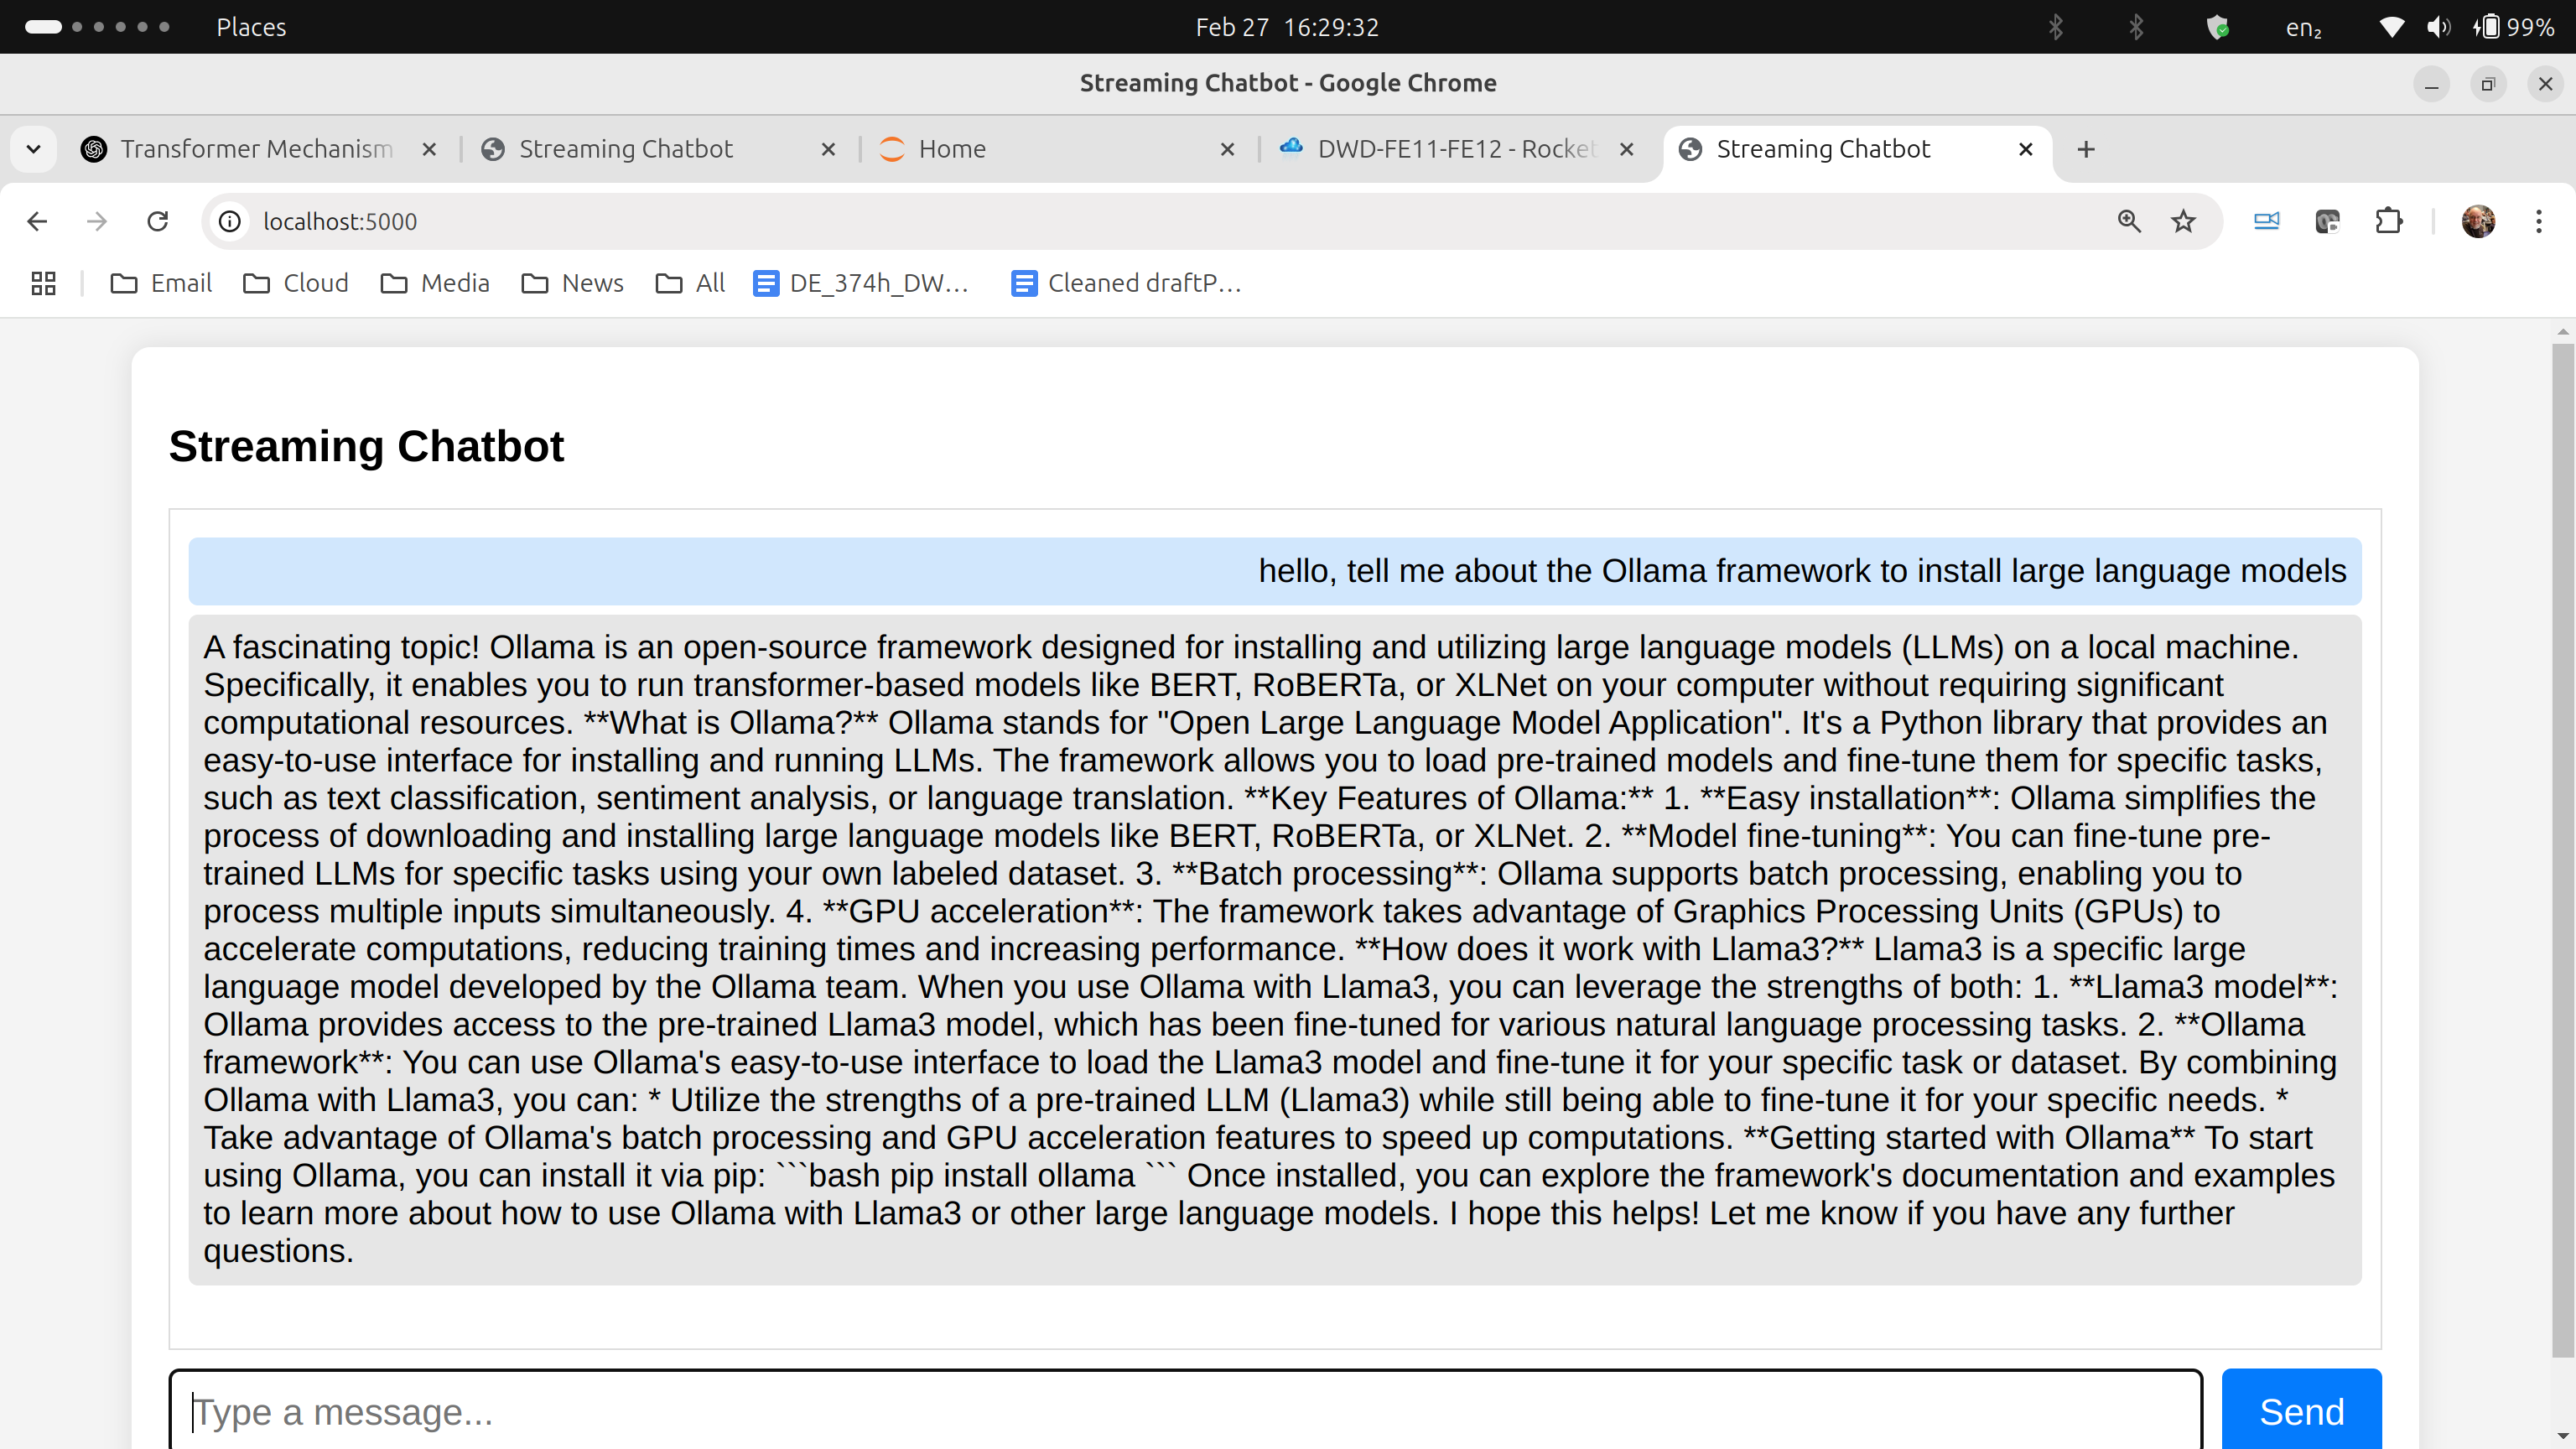
\includegraphics[width=0.8\textwidth]{images/ollama_chatbot.png}
    \caption{Ollama chatbot interface running a local LLM on your laptop, with local UI.}
    \label{fig:ollama_chatbot}
\end{figure}

Once the server is running, you should see output like:

\begin{codeonly}{Server Output}
 * Running on http://127.0.0.1:5000/ (Press CTRL+C to quit)
\end{codeonly}

\subsubsection{Accessing the User Interface}

To interact with the chatbot, open a web browser and go to:

\begin{codeonly}{Accessing the UI}
http://127.0.0.1:5000/
\end{codeonly}

From there, you can enter messages in the input field, and the chatbot will respond accordingly.
This simple local chat UI provides an easy way to interact with Ollama using a web-based interface while maintaining personal chat history.

%==============================================================================
%
%==============================================================================
\subsection{Streaming Responses from Ollama with Markdown Formatting}

In interactive environments such as Jupyter Notebooks or user interfaces (UI), it can be beneficial to stream responses from Ollama in real time while applying Markdown formatting to be able to display e.g. bold words or headings. The following example demonstrates how to achieve this using Python.

The function \texttt{stream\_ollama\_markdown()}:
\begin{itemize}
    \item Sends a request to a locally running Ollama server.
    \item Receives responses in a streaming fashion.
    \item Formats the output dynamically using Markdown to enhance readability.
    \item Updates the output in place without reloading the cell.
\end{itemize}

The function \texttt{format\_markdown()} ensures that:
\begin{itemize}
    \item Capitalized words and model names are bolded for emphasis.
    \item Titles such as "Model Features:" are converted into Markdown headings.
    \item Lists are properly formatted for readability.
\end{itemize}

The demo implementation is given below:

\begin{codeonly}{Streaming Markdown Output from Ollama}
import requests
import json
import re
from IPython.display import display, Markdown, clear_output

def format_markdown(text):
    text = text.replace("\n", "\n\n")
    text = re.sub(r'\b([A-Z][a-z]+(?:\s+[A-Z][a-z]+)*)\b', r'**\1**', text)
    text = re.sub(r'\b([A-Z]{3,})\b', r'**\1**', text)
    return text

def stream_ollama_markdown(prompt, model="llama3"):
    url = "http://localhost:11434/api/generate"
    data = {"model": model, "prompt": prompt, "stream": True}

    response = requests.post(url, json=data, stream=True)
    buffer = ""
    output_display = display(Markdown(""), display_id=True)

    for chunk in response.iter_lines():
        if chunk:
            try:
                data = json.loads(chunk.decode("utf-8"))
                text = data.get("response", "")
                if text:
                    buffer += text
                    clear_output(wait=True)
                    output_display.update(Markdown(format_markdown(buffer)))
            except json.JSONDecodeError:
                pass

    # Final display (in case last chunk isnt shown)
    clear_output(wait=True)
    output_display.update(Markdown(format_markdown(buffer)))
    # No return


# Try it
stream_ollama_markdown("Explain the concept of self-attention in Transformers.")

\end{codeonly}

This method enables seamless streaming of responses from Ollama, allowing for an interactive and visually structured output in Jupyter environments.
We also provide a demo implementation of a streaming interface for your flask based user interface (UI) to Ollama, see \texttt{ollama\_flask\_server\_streaming.py} with the \texttt{index\_stream.html} in the \texttt{templates/} directory. 

%==============================================================================


\subsection{Available Models for Download and Response Speed}

There are more than 150 different LLMs for download and use on Ollama. Here is a selection with some highlighted features. 

\begin{enumerate}
    \item \textbf{DeepSeek-R1 (1.5B – 671B)}  
    A powerful model family covering a wide range of sizes, from small-scale 1.5B to massive 671B parameters, making it flexible for different applications.
    
    \item \textbf{Llama3 (8B, 70B)}  
    One of the most anticipated next-generation models from Meta, optimized for efficiency and capable of handling diverse NLP tasks with strong performance.
    
    \item \textbf{Mistral (7B)}  
    A lightweight model with excellent reasoning capabilities, outperforming many larger models in specific tasks while remaining efficient.
    
    \item \textbf{Qwen2.5 (0.5B – 72B)}  
    Alibaba’s Qwen models are designed for multilingual tasks and reasoning, with a focus on applications requiring high levels of comprehension.
    
    \item \textbf{CodeLlama (7B – 70B)}  
    An LLM specifically optimized for code generation and software development, making it useful for programmers and AI-assisted coding.
    
    \item \textbf{Gemma (2B, 7B)}  
    Google’s Gemma models are efficient and optimized for deployment, designed for responsible AI usage and fine-tuned performance.
    
    \item \textbf{Mixtral (7B, 22B)}  
    A mixture-of-experts (MoE) model that enables highly efficient inference while maintaining competitive accuracy in language tasks.
    
    \item \textbf{Starcoder2 (3B – 15B)}  
    A coding model built for AI-assisted development, capable of understanding and generating code efficiently across multiple programming languages.
    
    \item \textbf{Orca Mini (3B – 70B)}  
    A distilled model trained with advanced reasoning capabilities, making it an excellent option for lightweight yet powerful AI assistants.
    
    \item \textbf{Llava (7B – 34B)}  
    A vision-language model capable of understanding images along with text, useful for applications in multimodal AI tasks like captioning and visual question answering.
\end{enumerate}

\begin{figure}[h]
    \centering
    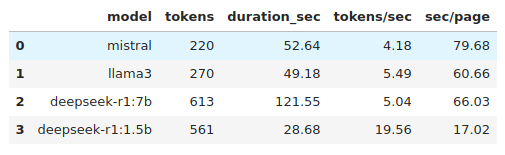
\includegraphics[width=0.8\textwidth]{images/token_per_second.png}
    \caption{Ollama on windows wsl on a regular workstation or laptop. With a light NVIDIA GPU (4GB) speed is about 2.5 times faster. On a linux laptop I got 33 token per second for deepseek-r1:1.5b.}
    \label{fig:ollama_chatbot}
\end{figure}

Large Language Models (LLMs) have become increasingly accessible for local installations, enabling users to process text without relying on cloud services. One crucial performance metric for such models is their response time, typically measured in milliseconds per token.

The speed at which an LLM generates tokens depends on hardware capabilities, model size, and optimization techniques. The DeepSeek-R1:1.5B model on a typical Linux laptop generates one token every 30 milliseconds (ms). The number of tokens generated in a given time frame is given by:
\begin{equation}
    N = \frac{T}{t},
\end{equation}
where:
\begin{itemize}
    \item $N$ is the number of tokens,
    \item $T$ is the total time available (in ms),
    \item $t$ is the time per token (30 ms in this case).
\end{itemize}

For practical scenarios:
\begin{itemize}
    \item In one second ($T = 1000$ ms):
    \begin{equation}
        N = \frac{1000}{30} \approx 33.33 \text{ tokens per second}.
    \end{equation}
    \item In ten seconds ($T = 10000$ ms):
    \begin{equation}
        N = \frac{10000}{30} \approx 333.33 \text{ tokens in ten seconds}.
    \end{equation}
\end{itemize}

To estimate the text length corresponding to these tokens, we assume:
\begin{itemize}
    \item One token typically consists of about 4 characters (including spaces and punctuation).
    \item One token represents approximately 0.75 words in standard English text.
\end{itemize}
Thus, for 333 tokens:
\begin{itemize}
    \item Character count: \( 333 \times 4 = 1332 \) characters.
    \item Word count: \( 333 \times 0.75 \approx 250 \) words.
\end{itemize}
This corresponds to roughly one page of text in a typical document.

The response time of an LLM either online as a service or installed on a local computer significantly influences usability. At 30 ms per token, the DeepSeek-R1:1.5B model can generate around 33 tokens per second or 250 words in ten seconds. Optimizing performance with hardware acceleration (e.g., GPUs, tensor cores) can further improve these figures, making local AI processing a viable alternative to cloud-based models.

\begin{recommendationbox}
Today, medium size LLMs can be run for individual users on a laptop, with acceptable response times for interactive applications. Alternatively and depending on privacy needs the use of platform accounts by AI companies provides faster access to the basic LLM functionality. User services based on either locally or remotely hosted LLM functionality is at hand and can be combined with specific local services and data. 
\end{recommendationbox}
 % 

\addtocontents{toc}{\noindent\hrulefill\vspace{-1.5ex}\par}
\addcontentsline{toc}{chapter}{\textcolor{dwdspecial}{\large Day 3: LLM RAG, Python Packages, Multi-Modality}}


\chapter{LLM with Retrieval-Augmented Generation (RAG)}
Retrieval-Augmented Generation (RAG) is a powerful approach that enhances language models by incorporating external knowledge retrieval. This chapter guides the user through setting up and using RAG, with practical examples.

{\bf Introduction to RAG}
Traditional LLMs rely solely on their pre-trained knowledge. RAG extends this by searching a document database for relevant context before generating a response. This improves accuracy, factuality, and adaptability to domain-specific knowledge.

\begin{figure}[ht]
    \centering
    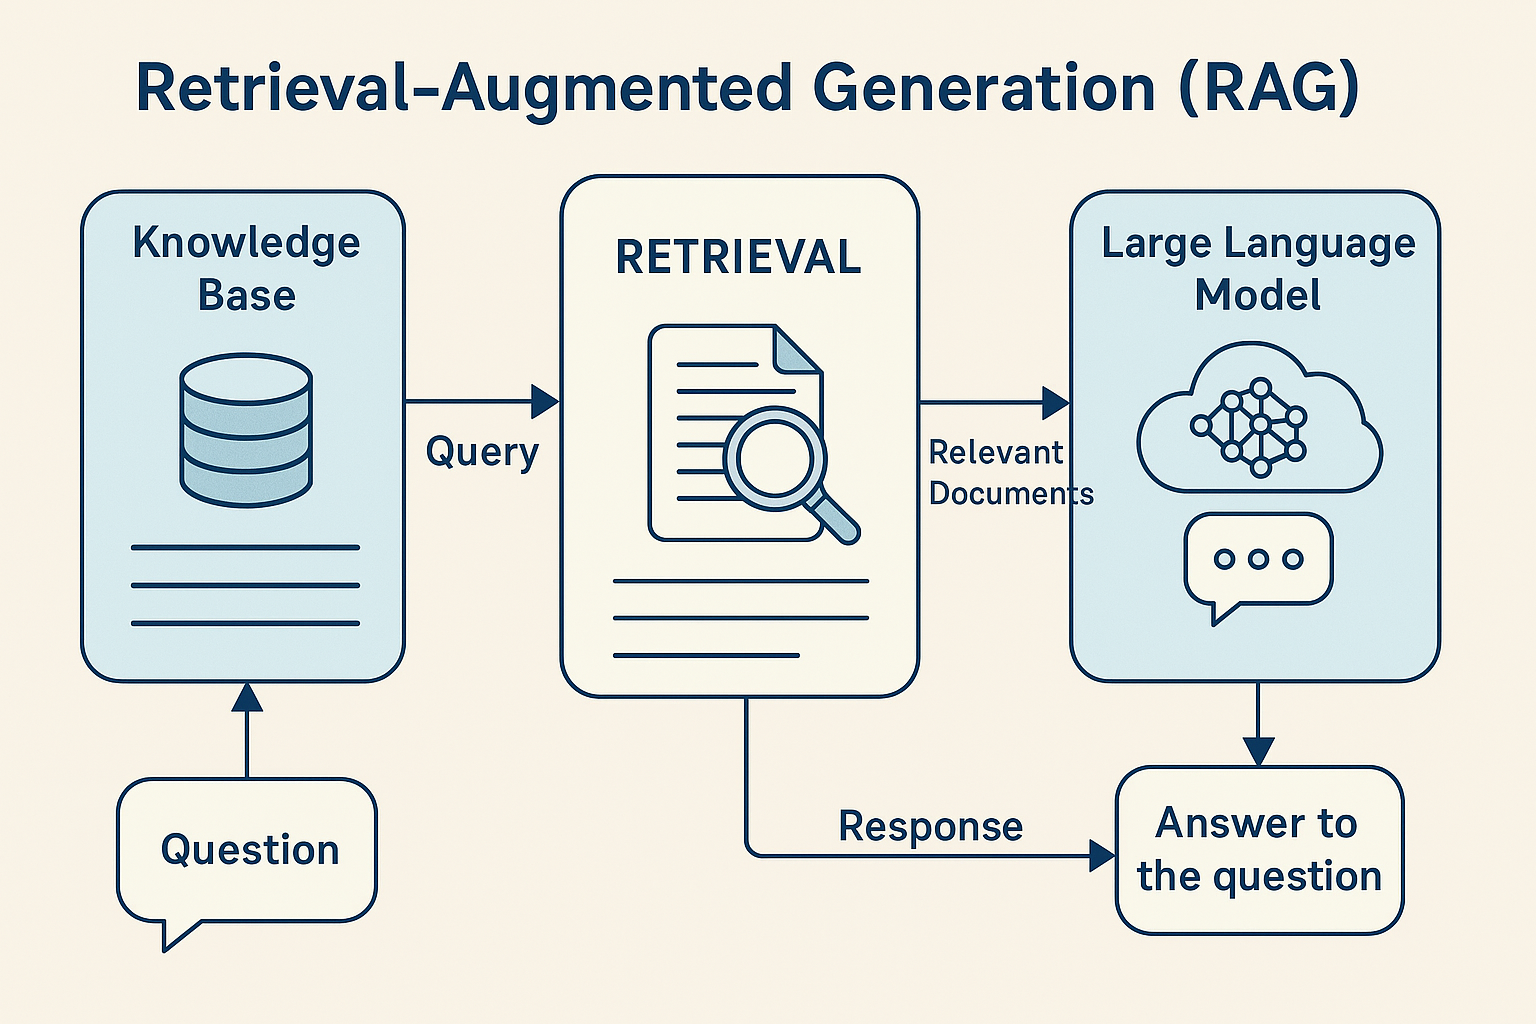
\includegraphics[width=0.7\textwidth]{images/RAG.png}
    \caption{Retrieval-Augmented Generation (RAG) employs the intelligence of Large Language Models (LLM) in combination with local knowledge and databases.}
    \label{fig:vectordb_out}
\end{figure}

%==============================================================================
%
%==============================================================================
\section{Preparing Documents}


{\bf Installing Required Dependencies}
To set up RAG, install the necessary libraries:

\begin{codeonly}{Install Dependencies}
!pip install sentence-transformers==2.2.2 transformers==4.31.0
!pip install faiss-cpu openai numpy pymupdf
\end{codeonly}
To get compatible versions of transformers and sentence-transformers might be a little tricky. I had to go back to python3.11 to get this running in a special virtual environment. 

First, let us work with documents which are in a folder tree starting with its root node \texttt{documents/}. 
We start by recursively loading text and PDF documents from this folder, marching through the tree. For pdf documents, we will use some standard tools to extract the text from the documents - there are more sophisticated packages, but we put simplicity first for the moment.  

\begin{codeonly}{Loading Documents}
import numpy as np
import os
import fitz  # PyMuPDF for PDF text extraction

# Function to extract text from PDF
def extract_text_from_pdf(pdf_path):
    doc = fitz.open(pdf_path)
    text = ""
    for page in doc:
        text += page.get_text()
    return text

# Load documents from a folder recursively
def load_documents_from_folder(folder_path):
    documents = []
    file_info = []
    
    for dirpath, dirnames, filenames in os.walk(folder_path):
        # Exclude .git directories
        dirnames[:] = [d for d in dirnames if not d.startswith('.git')]

        for filename in filenames:
            if filename.startswith('.git'):
                continue  # Skip any .git files

            file_path = os.path.join(dirpath, filename)
            if filename.endswith(('.f90','.txt', '.org', '.sh', '.toml','.pdf')) \
                or '.' not in filename:  # Load .txt, .sh, .pdf, and files without extensions
                try:
                    if filename.endswith('.pdf'):
                        content = extract_text_from_pdf(file_path)
                    else:
                        with open(file_path, 'r', encoding='utf-8') as file:
                            content = file.read()
                    documents.append(content)
                    file_info.append((filename, file_path))
                    print(f"Added to DB: {file_path}")
                except Exception as e:
                    print(f"Failed to process {file_path}: {e}")
    
    return documents, file_info
\end{codeonly}

We call the function to load all available documents by 

\begin{codeonly}{Loading Documents}
folder_path = './documents'  # Replace with your folder path
documents, file_info = load_documents_from_folder(folder_path)
\end{codeonly}

As an example we checkout the publically available ICON model by
\begin{codeonly}{Checkout ICON model}
git clone git@gitlab.dkrz.de:icon/icon-model.git
\end{codeonly}

In this case, the output is
\begin{codeonly}{ICON model from icon-model.org loaded}
Added to DB: ./documents/configure
Added to DB: ./documents/make_runscripts
Added to DB: ./documents/utils/install-sh
Added to DB: ./documents/utils/move_to_prefix.sh
Added to DB: ./documents/utils/patch_namelist
Added to DB: ./documents/utils/timewarp
Added to DB: ./documents/utils/icon_sorted_deps.sh
Added to DB: ./documents/utils/id++
Added to DB: ./documents/utils/filelock
Added to DB: ./documents/utils/mkexp/namelist2config
Added to DB: ./documents/utils/mkexp/mkexp
Added to DB: ./documents/utils/mkexp/upexp
Added to DB: ./documents/utils/mkexp/unmergeconfig
Added to DB: ./documents/utils/mkexp/selconfig
Added to DB: ./documents/utils/mkexp/importexp
Added to DB: ./documents/utils/mkexp/editexp
...
\end{codeonly}




%==============================================================================
%
%==============================================================================
\section{Generating Embeddings for Documents}

To retrieve relevant information, we transform text into \textbf{numerical embeddings} using a \textbf{transformer model}. These embeddings capture the \textit{semantic meaning} of text, allowing for similarity-based retrieval and efficient search operations. A widely used approach for generating such embeddings is \textbf{sentence transformers}, which map textual data into a high-dimensional vector space.

In the following implementation, we utilize the \texttt{all-MiniLM-L6-v2} model from the \texttt{sentence-transformers} library. This model provides a compact yet efficient method for encoding textual information. The embeddings are computed using \textbf{mean pooling} over the token representations, ensuring that the vector captures the full meaning of the sentence. Additionally, we apply \textbf{L2 normalization} to facilitate cosine similarity comparisons.

\begin{codeonly}{Generating Embeddings}
from sentence_transformers import SentenceTransformer

embedder = SentenceTransformer('all-MiniLM-L6-v2')

# Load documents and create embeddings
documents, file_info = load_documents_from_folder("documents/")
embeddings = embedder.encode(documents, convert_to_numpy=True)

# Sanity check
print("Loaded documents:", len(documents))
print("Embedding shape:", embeddings.shape)
print("Example file:", file_info[0])
print("Example snippet:\n", documents[0][:200])
\end{codeonly}

The function \texttt{embedder.encode} tokenizes the input text, processes it through the transformer model, and computes a \textbf{mean-pooled representation} over the token dimension. The final embeddings are \textbf{normalized}, ensuring that similarity computations (e.g., cosine similarity) remain well-scaled.

Such embeddings enable applications in \textbf{semantic search}, \textbf{clustering}, and \textbf{document classification} by mapping textual data into a structured numerical space that can be efficiently queried.

In our case we obtain
\begin{codeonly}{Check embeddings}
Loaded documents: 2391
Embedding shape: (2391, 384)
Example file: ('make_runscripts', 'documents/make_runscripts')
Example snippet:
 #! /bin/bash

# ICON
#
# ------------------------------------------
# Copyright (C) 2004-2024, DWD, MPI-M, DKRZ, KIT, ETH, MeteoSwiss
# Contact information: icon-model.org
# See AUTHORS.TXT for a list
\end{codeonly}

Our embeddings variable has a shape of (2391, 384), which means there are 
2391 rows, i.e.\ 2391 text inputs (documents, sentences, or paragraphs). We have
384 columns, i.e.\ each text input is represented as a 384-dimensional vector.

{\bf How the Embeddings Work.}
The closer two embeddings are (e.g., using cosine similarity), the more semantically similar their corresponding texts are.
The high-dimensional space (384D) allows the model to capture complex semantic relationships between texts.

\bigskip
{\bf Retrieving Relevant Documents}
When a user asks a question, we find the most relevant documents by searching the FAISS index.

\begin{codeonly}{Querying the Vector Database}
def query_vector_db(query, k=2):
    query_embedding = get_embedding(query)
    distances, indices = index.search(query_embedding, k)
    return [documents[idx] for idx in indices[0]]

query = "What is the main functionality of BACY?"
retrieved_docs = query_vector_db(query)
print(retrieved_docs)
\end{codeonly}

{\bf Setting Up a Vector Database with FAISS}
To efficiently search for similar text embeddings, we store them in a {\bf FAISS index}. FAISS (Facebook AI Similarity Search) is an optimized library for fast {\bf nearest neighbor search} in high-dimensional spaces. Instead of performing a brute-force comparison of all pairs of embeddings, FAISS allows us to {\em index and retrieve} the most relevant embeddings efficiently.

FAISS supports different types of indexes, but the most basic and commonly used one is 
\textbf{IndexFlatL2}, which stores vectors and enables fast \textit{k}-nearest neighbor (KNN) search using the {\em L2 (Euclidean) distance}.

\begin{codeonly}{Setting Up FAISS Index}
import faiss

# Create FAISS index
dimension = embeddings.shape[1]
index = faiss.IndexFlatL2(dimension)
index.add(embeddings)
\end{codeonly}

The \texttt{IndexFlatL2} structure is an exact nearest-neighbor search index that:
\begin{itemize}
    \item Stores all embeddings in memory.
    \item Computes pairwise distances using **L2 norm (Euclidean distance)**.
    \item Allows fast similarity search without additional quantization.
\end{itemize}

{\bf Querying the FAISS Index.} 
Once the FAISS index is built, we can {\em perform similarity searches} by converting a text query into an embedding and retrieving the \( k \)-nearest neighbors from the indexed documents. The following function allows querying the vector database and retrieving the most relevant documents.

\begin{codeonly}{Querying the FAISS Index}
# Query function
def query_vector_db(query, k=2):
    """
    Searches the FAISS index for the k most similar embeddings to the query.

    Parameters:
    query (str): Input text to search for similar documents.
    k (int): Number of nearest neighbors to retrieve.

    Returns:
    list of tuples: Each tuple contains (retrieved_document, file_info).
    """
    query_embedding = get_embedding(query).astype(np.float32)  # Convert to FAISS format
    distances, indices = index.search(query_embedding, k)  # Perform similarity search
    return [(documents[idx], file_info[idx]) for idx in indices[0]]
\end{codeonly}

To demonstrate how the FAISS search works, we run an example query:

\begin{codeonly}{Example Query to FAISS}
import re
import unicodedata

def clean_text(text, max_chars=500):
    text = unicodedata.normalize("NFC", text)  # Normalize Unicode
    text = ''.join(c if c.isprintable() else ' ' for c in text)  # Keep printable chars
    return re.sub(r'\s+', ' ', text).strip()[:max_chars].encode("utf-8", "ignore").decode("utf-8")

# Example usage
query_text = "Cloud cover intro"
results = query_vector_db(query_text, k=6)

for doc, info in results: 
    print("File Info:", clean_text(str(info)))
    print("\nDocument:", clean_text(doc))
    print("-" * 50)
\end{codeonly}

This example queries the FAISS index for the {\em top $k$ most relevant documents} related to the weather forecast. The function:
\begin{itemize}
    \item Converts the input query into an {\em embedding}.
    \item Searches the FAISS index for the \( k \) most similar embeddings.
    \item Returns the corresponding {\bf documents and metadata}.
\end{itemize}

By retrieving the closest matches, we enable {\em semantic search}, allowing users to find {\em contextually similar documents} rather than relying on simple keyword matching. For our ICON example where we ask for {\em Cloud cover intro} we get the results indicated in Figure \ref{fig:vectordb_out}.  

\begin{figure}[ht]
    \centering
    
\includegraphics[width=\textwidth]{images/vectordb_out3.pdf}
    \caption{Vector Database Output}
    \label{fig:vectordb_out}
\end{figure}


%==============================================================================
%
%==============================================================================
\section{Using an LLM Locally or with OpenAI for Response Generation}

Once we retrieve relevant documents, we provide them as context to OpenAI’s LLM or any other large language model. 
This allows us to enhance responses with domain-specific information and improve accuracy.

\textbf{Setting up OpenAI API.} To use OpenAI, we need an \emph{OpenAI platform account} and an API key (\texttt{OPENAI\_API\_KEY}). 
If you have stored this key as an environment variable, you can initialize the API client as follows:

\begin{codeonly}{Connection to OpenAI}
import openai
import os

# Initialize OpenAI API
client = openai.Client(api_key=os.getenv('OPENAI_API_KEY'))  # Updated API initialization
\end{codeonly}

If no error occurs, the API connection is successfully established.

\textbf{Querying OpenAI with Retrieved Context.} Once we have access to OpenAI's API, we can define a function to query the model.
The function \emph{retrieves relevant documents} from our vector database and passes them as context to the model.
This enables OpenAI to provide responses based on our own data rather than generic knowledge. Here, we will employ the model {\em gpt-4o-mini} which is known for its speed and which is much cheaper than the flagship models. 

\begin{codeonly}{Generating Responses with OpenAI}
# Step 6: Use OpenAI to discuss results
def chat_with_openai(query):
    retrieved_docs = query_vector_db(query,k=20)
    context = "\n\n".join([f"File: {file[0]}\nContent: {doc}" for doc, file in retrieved_docs])
    
    response = client.chat.completions.create(
        model="gpt-4o-mini",  # using the gpt-4o-mini model
        messages=[
            {"role": "system", "content": "You are a helpful assistant."},
            {"role": "user", "content": f"Based on the following documents, answer the question:\n{context}\n\nQuestion: {query}"}
        ]
    )
    
    answer = response.choices[0].message.content
    
    # Append file references to the answer
    file_references = "\n\nReferenced Files:\n" + "\n".join([f"{file[0]}: {file[1]}" for _, file in retrieved_docs])
    
    return answer + file_references
\end{codeonly}

\textbf{How it works.} The function \texttt{chat\_with\_openai(query)} operates as follows:
\begin{itemize}
    \item \emph{Retrieves relevant documents} using the \texttt{query\_vector\_db(query, k=20)} function.
    \item \emph{Formats} the retrieved text into a structured context.
    \item \emph{Sends the context} to OpenAI’s model, prompting it to answer the query based on the retrieved content.
    \item \emph{Returns the generated response}, along with file references for transparency.
\end{itemize}

\textbf{Example query.} If a user searches for a specific topic, such as:

\begin{codeonly}{Example Query Execution}
# OpenAI Answers
query = "How is cloud cover treated in ICON?"
answer = chat_with_openai(query)

from IPython.display import display, Markdown
display(Markdown(answer))
\end{codeonly}

This ensures that OpenAI generates responses grounded in \emph{our own database}, reducing hallucination and improving relevance.

Here, the result for our example is as follows. 

\begin{lstlisting}[language=]
The ICON (ICOsahedral Nonhydrostatic) model is a state-of-the-art atmospheric model developed for weather and climate simulations. Its structure is designed to efficiently handle both global and regional simulations, including various atmospheric and surface physics processes. Below is an overview of its key components and architecture:

1. Grid Structure
Horizontal Grid: ICON uses a spherical grid based on the projection of an icosahedron. This grid can be refined through edge bisection, leading to triangular or hexagonal elements. The horizontal representation allows high resolution and flexibility in grid configuration.
Vertical Grid: The vertical structure uses hybrid coordinates, where the atmosphere is discretized into horizontal layers. These vertical layers can be based on pressure or height coordinates, accommodating both hydrostatic and non-hydrostatic dynamics.
2. Core Components
Dynamics: ICON features a non-hydrostatic dynamical core that enables accurate simulations of complex atmospheric phenomena, such as storms and convective processes. It employs a C-staggering scheme for state variables to improve computational efficiency, especially for advection and momentum transport.
Physics: The model integrates various physics packages for parameterizing physical processes. This includes:
Cloud microphysics to simulate cloud formation and precipitation.
Radiation schemes (like RRTMG) to calculate the transfer of solar and terrestrial radiation.
Convection schemes to model the vertical transport of heat and moisture in the atmosphere.
Surface processes involving land-atmosphere interactions, including soil moisture and vegetation effects.
3. Parallelization
ICON is designed for high-performance computing environments, utilizing both MPI (Message Passing Interface) and OpenMP for parallelization. This allows it to run efficiently on modern supercomputers, accommodating large-scale simulations with many processors.
4. Namelists
The configuration of the ICON model is managed through namelists, which are structured text files containing parameters for different aspects of the model. This includes settings for grid configurations, physics schemes, and output specifications.
5. Modules and Naming Conventions
The code is organized into modules for different functionalities (such as dynamics, radiation, and microphysics). Each module contains subroutines and functions that handle specific tasks. A clear naming convention is followed for ease of understanding, with prefixes used to indicate the nature and scope of variables.
6. Output and Diagnostics
ICON is equipped with flexible output capabilities that can generate various diagnostic fields related to atmospheric states and physical processes, including radar reflectivity and cloud cover. Output can be tailored to specific requirements utilizing naming conventions for files and variable names.
7. Community and Documentation
The development of ICON follows best coding practices as outlined in guidelines for readability and maintainability. The model is supported by detailed documentation, ensuring users can effectively configure and use the model for their research needs.
8. External Packages
ICON can integrate with external libraries and frameworks for additional functionalities, allowing for advanced features like data assimilation and coupling with ocean models.
In summary, the ICON model embodies a sophisticated structure that combines modern computational techniques with detailed atmospheric science, enabling high-resolution weather and climate simulations across a range of applications. Its modular architecture and parallel processing capabilities make it suitable for use in both research and operational forecasting environments.

Referenced Files: [...]
\end{lstlisting}

An alternative to OpenAI's API is to use \emph{Ollama}, which allows running large language models locally. 
This provides greater control over data privacy and removes dependency on external services. 
The following function queries a locally hosted model, such as \texttt{Mistral} or \texttt{DeepSeek-R1:1.5b}, 
using retrieved documents from the vector database.

\begin{codeonly}{Querying Ollama Locally}
import ollama

def chat_with_ollama(query, model="mistral"):
    """Queries Ollama's local LLM (Mistral or DeepSeek) with retrieved VectorDB documents."""
    retrieved_docs = query_vector_db(query, k=20)
    context = "\n\n".join([f"File: {file[0]}\nContent: {doc}" for doc, file in retrieved_docs])

    full_prompt = f"Based on the following documents, answer the question:\n{context}\n\nQuestion: {query}"

    response = ollama.chat(model=model, messages=[{"role": "user", "content": full_prompt}])

    answer = response['message']['content']

    # Append file references
    file_references = "\n\nReferenced Files:\n" + "\n".join([f"{file[0]}: {file[1]}" for _, file in retrieved_docs])

    return answer + file_references
\end{codeonly}

The function first retrieves relevant documents from the vector database and formats them into a structured prompt. 
It then queries a local Ollama instance running the selected model and appends file references to ensure traceability.

The following examples demonstrate how to use \texttt{DeepSeek-R1:1.5b} and \texttt{Mistral} to answer a query 
regarding the structure of the ICON model.

\begin{codeonly}{Example Query with DeepSeek-R1:1.5b}
query_text = "Tell me about the structure of the ICON model"
answer = chat_with_ollama(query_text, model="deepseek-r1:1.5b")

# Display response as formatted Markdown
display(Markdown(answer))
\end{codeonly}

\begin{codeonly}{Example Query with Mistral}
answer = chat_with_ollama(query_text, model="mistral")

# Display response as formatted Markdown
display(Markdown(answer))
\end{codeonly}

This approach allows flexible switching between different local models, depending on the required accuracy, speed, or computational efficiency. It works locally on your laptop, but might take slightly longer for answers. 

Here is the deepseek answer: 

\begin{lstlisting}[language=]
Alright, I need to tell someone about the structure of the ICON model. Let's break this down step by step.
First, I should recall what the ICON model is. From my limited knowledge, it's a global numerical weather prediction model used for atmospheric simulations. The user mentioned various files like balfringpu_nvidia and others related to it. These probably contain the source code and documentation.

Looking at the files provided:

[...]
In summary, understanding the ICON model involves knowing its architecture, how it processes data through various components, and the parameters that control this processing. The structure is complex yet modular, allowing for detailed physical modeling on a global scale.

The ICON (Icosahedral Non-Oceanic Model) model is a global numerical weather prediction system designed to simulate atmospheric circulation. Here's its structured overview:

Structure of the ICON Model
Configuration Management:

[...]

Computes forward in time using processes like hydrostatic pressure, moist static stability, gravity wave propagation, advection, radiation, etc.
Utilizes parallelization on high-performance computing clusters for efficiency.
Key Features
High Scalability: Designed for efficient computation on clusters of CPUs.
Global Coverage: Serves as a foundational component for weather models.
Flexibility: Adjustable parameters allow customization for specific applications.
The ICON model's structure is modular, managing data through components that ensure accurate and scalable global atmospheric modeling.

Referenced Files: [...] Namelist_overview.pdf: ./documents/doc/Namelist_overview.pdf icon_grid.pdf: ./documents/doc/technical/icon_grid.pdf dot_cdprc: ./documents/schedulers/ecmwf/gen/dot_cdprc icon_standard.pdf: ./documents/doc/style/icon_standard.pdf [...]
\end{lstlisting}


%==============================================================================
%
%==============================================================================
\section{Saving and Reloading the Vector Database, Collecting Search Originals, Chunking long Documents}
To avoid recomputing embeddings every time, we save the FAISS index to disk. 
This allows us to reload it efficiently for future searches.

\begin{codeonly}{Saving and Loading FAISS Index}
import faiss
import os

# Save FAISS index
faiss.write_index(index, "vector_db.index")
print("Vector database saved.")

# Ensure file exists before loading
if os.path.exists("vector_db.index"):
    index = faiss.read_index("vector_db.index")
    print("Vector database loaded.")
else:
    print("Error: FAISS index file not found.")
\end{codeonly}

This method ensures that the FAISS index persists across sessions, eliminating the need for 
recomputing embeddings. If additional metadata, such as document mappings, is needed, 
they must be stored separately in a structured format (e.g., JSON or a database).

\bigskip
{\bf Search Results: Documents.}
Often it can be helpful to look into the results of a search directly. The following code saves all retrieved 
documents into a designated results folder, while ensuring previous results are backed up by renaming the 
existing folder.

\begin{codeonly}{Save Search Documents}
import os
import shutil

def backup_and_create_results_folder(base_folder="results"):
    """Backs up existing results folder by renaming it to results_nnn and creates a new empty folder."""
    
    if os.path.exists(base_folder):
        counter = 1
        while os.path.exists(f"{base_folder}_{counter:03d}"):
            counter += 1
        backup_folder = f"{base_folder}_{counter:03d}"
        shutil.move(base_folder, backup_folder)
        print(f"Existing results folder backed up as: {backup_folder}")

    os.makedirs(base_folder, exist_ok=True)
    return base_folder

def copy_retrieved_documents(query, k=10, results_folder="results"):
    """Finds relevant documents using FAISS and copies them to the results folder, saving the query."""
    
    # Backup old results and create new folder
    results_folder = backup_and_create_results_folder(results_folder)

    # Retrieve relevant documents
    retrieved_docs = query_vector_db(query, k)
    
    copied_files = []
    
    for _, file_info in retrieved_docs:
        file_path = file_info[1]  # Assuming file_info[1] contains the file path

        if os.path.exists(file_path):
            dest_path = os.path.join(results_folder, os.path.basename(file_path))
            shutil.copy(file_path, dest_path)
            copied_files.append(dest_path)
        else:
            print(f"Warning: File not found - {file_path}")

    # Save query text
    query_path = os.path.join(results_folder, "query.txt")
    with open(query_path, "w", encoding="utf-8") as f:
        f.write(query)
    
    print(f"Copied {len(copied_files)} files to {results_folder}")
    print(f"Query saved in {query_path}")
\end{codeonly}

\bigskip
{\bf Example Usage.}
The following example retrieves documents related to turbulence schemes in ICON and saves them in the 
results folder.

\begin{codeonly}{Example Query and Document Copy}
query_text = "What turbulence scheme in ICON?"
copy_retrieved_documents(query_text, k=20)
\end{codeonly}

\bigskip
{\bf Displaying the Retrieved Files.}
Once the search is complete, the saved documents can be listed to verify their contents. The following 
example shows the typical contents of the results folder after a search.

\begin{lstlisting}[language=]
alps_mch_test_gpu         daint_cpu_cce           flux_diagram-crop.pdf  icon_atm_echam_phy_scidoc.pdf  icon_technical.pdf    NOTICE
AUTHORS.txt               daint_cpu_nvidia_mixed  flux_diagram.pdf       icon_grid.pdf                  icon_tuning_vars.pdf  query.txt
balfrin_gpu_nvidia_mixed  dep5                    horeka_cpu_nvhpc       icon_standard.pdf              lmclouds2010.pdf      README
\end{lstlisting}

This setup ensures that all relevant documents are efficiently stored, organized, and available for analysis.

\bigskip
{\bf Adding some Tutorial to the Search Database.}
Providing only some code base is often not sufficient to understand it. One important step is to add more targeted material to the search. 

Often some tutorial is available online but is not part of the source code repository. To ensure efficient retrieval, we split the tutorial into small chunks, embed each chunk, and add them to the FAISS vector database.

\begin{codeonly}{Processing ICON Tutorial to get pages}
from PyPDF2 import PdfReader

def extract_pages_from_pdf(pdf_path):
    """Reads a PDF and returns a list of page texts."""
    reader = PdfReader(pdf_path)
    return [page.extract_text() for page in reader.pages]

# Load the tutorial as separate pages
tutorial_pdf = "ai_tutorial.pdf"
tutorial_pages = extract_pages_from_pdf(tutorial_pdf)

# Check output
print(f"Extracted {len(tutorial_pages)} pages.")
\end{codeonly}

\begin{codeonly}{Chunking and Embedding}
tutorial_embeddings = np.vstack([get_embedding(page) for page in tutorial_pages])

tutorial_file_name = "ai_tutorial.pdf"
tutorial_page_refs = [f"{tutorial_file_name} - Page {i+1}" for i in range(len(tutorial_pages))]

# Add to main lists
documents.extend(tutorial_pages)
file_info.extend([(ref, tutorial_file_name) for ref in tutorial_page_refs])

index.add(tutorial_embeddings)
\end{codeonly}

This ensures that the tutorial is available for search queries, returning relevant sections instead of 
requiring manual document lookup. Here, I added a draft of the AI tutorial you are reading. 

\begin{codeonly}{Query with Code and Tutorial included}
# OpenAI Answers
query = "What NN architectures did we talk about? CNN? GNN? Transformers?"
answer = chat_with_openai(query)

from IPython.display import display, Markdown
display(Markdown(answer))
\end{codeonly}

OpenAI with gpt-4o-mini comes with the following answer: 

\lstset{language=}
\begin{lstlisting}
Based on the documents provided, the discussed neural network (NN) architectures include:

Feedforward Neural Networks (FFNN) - The simplest form of artificial neural networks where information moves in one direction from the input layer through hidden layers to the output layer.

Convolutional Neural Networks (CNN) - Powerful architectures typically used for image processing and can be applied to one-dimensional data, such as time series and function classification.

Recurrent Neural Networks (RNN) - Particularly highlighted for sequence learning, with types like Long Short-Term Memory (LSTM) networks, which improved the processing of language sequences.

Transformers - Introduced groundbreaking innovations with self-attention mechanisms and parallel processing, becoming the standard for modern language models.

The documents specifically mention CNNs and Transformers, while RNNs (including LSTMs) are noted for their advancements in sequence processing. There was no mention of Graph Neural Networks (GNN) in the provided materials.

Referenced Files: ai_tutorial.pdf - Page 5: ai_tutorial.pdf ai_tutorial.pdf - Page 188: ai_tutorial.pdf ai_tutorial.pdf - Page 111: ai_tutorial.pdf ai_tutorial.pdf - Page 182: ai_tutorial.pdf ai_tutorial.pdf - Page 101: ai_tutorial.pdf ai_tutorial.pdf - Page 90: ai_tutorial.pdf ai_tutorial.pdf - Page 124: ai_tutorial.pdf ai_tutorial.pdf - Page 130: ai_tutorial.pdf ai_tutorial.pdf - Page 113: ai_tutorial.pdf ai_tutorial.pdf - Page 192: ai_tutorial.pdf ai_tutorial.pdf - Page 190: ai_tutorial.pdf ai_tutorial.pdf - Page 102: ai_tutorial.pdf ai_tutorial.pdf - Page 191: ai_tutorial.pdf ai_tutorial.pdf - Page 87: ai_tutorial.pdf ai_tutorial.pdf - Page 120: ai_tutorial.pdf ai_tutorial.pdf - Page 131: ai_tutorial.pdf ai_tutorial.pdf - Page 114: ai_tutorial.pdf ai_tutorial.pdf - Page 193: ai_tutorial.pdf ai_tutorial.pdf - Page 126: ai_tutorial.pdf ai_tutorial.pdf - Page 167: ai_tutorial.pdf
\end{lstlisting}

Mistral is getting this as well in a very concise way. 

\begin{codeonly}{Mistral Query}
answer = chat_with_ollama(query, model="mistral")

# Display response as formatted Markdown
display(Markdown(answer))
\end{codeonly}

\lstset{language=}
\begin{lstlisting}
In this text, we talked about three types of neural network architectures: Convolutional Neural Networks (CNN), Graph Neural Networks (GNN), and Transformers. The CNN architecture was discussed in the context of image processing tasks, whereas Transformers were mentioned in relation to large language models and the self-attention mechanism. It appears that GNN wasn't directly addressed in this particular part of the text, but it could be inferred from other sections discussing graph-based problems like social network analysis or molecular simulations.

Referenced Files: ai_tutorial.pdf - Page 5: ai_tutorial.pdf ai_tutorial.pdf - Page 188: ai_tutorial.pdf ai_tutorial.pdf - Page 111: ai_tutorial.pdf ai_tutorial.pdf - Page 182: ai_tutorial.pdf ai_tutorial.pdf - Page 101: ai_tutorial.pdf ai_tutorial.pdf - Page 90: ai_tutorial.pdf ai_tutorial.pdf - Page 124: ai_tutorial.pdf ai_tutorial.pdf - Page 130: ai_tutorial.pdf ai_tutorial.pdf - Page 113: ai_tutorial.pdf ai_tutorial.pdf - Page 192: ai_tutorial.pdf ai_tutorial.pdf - Page 190: ai_tutorial.pdf ai_tutorial.pdf - Page 102: ai_tutorial.pdf ai_tutorial.pdf - Page 191: ai_tutorial.pdf ai_tutorial.pdf - Page 87: ai_tutorial.pdf ai_tutorial.pdf - Page 120: ai_tutorial.pdf ai_tutorial.pdf - Page 131: ai_tutorial.pdf ai_tutorial.pdf - Page 114: ai_tutorial.pdf ai_tutorial.pdf - Page 193: ai_tutorial.pdf ai_tutorial.pdf - Page 126: ai_tutorial.pdf ai_tutorial.pdf - Page 167: ai_tutorial.pdf
\end{lstlisting}

In general, chunking and decomposition of the material into good and adequate parts is a very important part of the whole process. The LLM has limited context size and using the right information is a crucial part of answering a query or taking part in a discussion.  %
\chapter{Python Packages}
Python has a rich ecosystem of libraries for scientific computing, data analysis, and geospatial processing. This chapter introduces important packages that complement Python’s core functionality, providing efficient tools for working with structured data, performing computations, and visualizing results.


\section{Review of the Python Standard Library}
Python includes a comprehensive standard library that provides built-in functionality for various tasks. The following table lists some of the most commonly used standard library modules:

\begin{center}
\begin{tabular}{|l|p{10cm}|}
\hline
\textbf{Module} & \textbf{Description} \\
\hline
os & Provides functions for interacting with the operating system. \\
sys & Gives access to system-specific parameters and functions. \\
math & Offers mathematical functions such as trigonometry, logarithms, and factorial. \\
random & Generates pseudo-random numbers and selections. \\
datetime & Handles date and time manipulation. \\
collections & Provides specialized container datatypes like namedtuples and defaultdicts. \\
itertools & Implements fast, memory-efficient iterators. \\
functools & Contains higher-order functions like memoization (lru\_cache). \\
json & Allows parsing and generation of JSON data. \\
tempfile & Creates temporary files and directories. \\
logging & Offers flexible logging utilities. \\
argparse & Parses command-line arguments. \\
shutil & Performs high-level file operations. \\
pathlib & Modern alternative to os.path for handling filesystem paths. \\
subprocess & Runs shell commands and external processes. \\
thre@ding & Provides concurrency using threads. \\
multiprocessing & Supports parallel execution of code. \\
asyncio & Provides asynchronous I/O and event loops. \\
http & Supports HTTP client and server operations. \\
urllib & Fetches data across the web. \\
sqlite3 & Provides a lightweight database engine. \\
re & Implements regular expressions. \\
\hline
\end{tabular}
\end{center}

\subsection{Working with the OS and Filesystem}
The \texttt{os} and \texttt{pathlib} modules allow interaction with the operating system and filesystem.

\begin{codeonly}{Listing Files in a Directory}
import os

# List all files in the current directory
files = os.listdir('.')
print(files)
\end{codeonly}

\begin{codeonly}{Using Pathlib for File Paths}
from pathlib import Path

# Create a path object and check if a file exists
path = Path("example.txt")
print("File exists:", path.exists())
\end{codeonly}

\subsection{Working with JSON Data}
The \texttt{json} module is used to parse and generate JSON data.

\begin{codeonly}{Parsing and Writing JSON Data}
import json

data = {"name": "Alice", "age": 30}
json_str = json.dumps(data)
print(json_str)

# Convert JSON string back to dictionary
decoded = json.loads(json_str)
print(decoded["name"])
\end{codeonly}

\subsection{Running External Commands}
The \texttt{subprocess} module allows running system commands from Python.

\begin{codeonly}{Executing a Shell Command}
import subprocess

# Run a shell command and capture its output
result = subprocess.run(["echo", "Hello, World!"], capture_output=True, text=True)
print(result.stdout)
\end{codeonly}

\subsection{Using Regular Expressions}
The \texttt{re} module provides powerful pattern matching capabilities.

\begin{codeonly}{Matching Patterns with Regular Expressions}
import re

text = "My email is example@example.com"
match = re.search(r"[\w.-]+@[\w.-]+", text)
if match:
    print("Found email:", match.group())
\end{codeonly}

This section has introduced key components of the Python standard library, demonstrating their practical usage through examples.


\section{Xarray - Multi-dimensional labled Data}
Xarray is a powerful library designed for working with multi-dimensional labeled data. It is particularly useful for handling NetCDF files and scientific datasets, making it an essential tool for climate and weather data analysis.

\subsection{Creating and Manipulating Xarray DataArrays}
An Xarray DataArray is a fundamental data structure representing labeled, multi-dimensional arrays.

\begin{codeonly}{Creating a DataArray}
import xarray as xr
import numpy as np

# Create a simple DataArray
data = np.random.rand(4, 3)
da = xr.DataArray(data, dims=("time", "location"), coords={"time": range(4), "location": ['A', 'B', 'C']})
print(da)
\end{codeonly}

\subsection{Using Xarray for NetCDF Files}
Xarray provides seamless integration with NetCDF files for reading and writing datasets.

\begin{codeonly}{Reading a NetCDF File}
dataset = xr.open_dataset("example.nc")
print(dataset)
\end{codeonly}

\begin{codeonly}{Writing a NetCDF File}
dataset.to_netcdf("output.nc")
\end{codeonly}

\subsection{Data Selection and Operations}
Xarray allows intuitive selection and computation on data.

\begin{codeonly}{Selecting Data by Coordinates}
selected = da.sel(time=2)
print(selected)
\end{codeonly}

\begin{codeonly}{Applying Mathematical Operations}
mean_value = da.mean(dim="time")
print(mean_value)
\end{codeonly}

\section{Pandas - Data Frames and Analysis Package}
Pandas is a fundamental package for data analysis, offering powerful tools for manipulating tabular data similar to spreadsheets or SQL databases.

\subsection{Creating DataFrames}

\begin{codeonly}{Creating a Pandas DataFrame}
import pandas as pd

data = {"A": [1, 2, 3], "B": [4, 5, 6]}
df = pd.DataFrame(data)
print(df)
\end{codeonly}

\subsection{Data Selection and Filtering}

\begin{codeonly}{Filtering Data}
filtered = df[df["A"] > 1]
print(filtered)
\end{codeonly}

\section{SciPy Scientific Computing, Optimization and Statistics}
SciPy extends NumPy with additional functionality for scientific computing, such as optimization, signal processing, and statistical analysis.

\subsection{Optimization Example}

\begin{codeonly}{Finding a Minimum Using SciPy}
from scipy.optimize import minimize

def func(x):
    return (x - 3) ** 2

result = minimize(func, x0=0)
print(result.x)
\end{codeonly}

\section{Scikit-Learn - Machine Learning, Classifiation, Regression}
Scikit-learn is a machine learning library that provides tools for classification, regression, clustering, and preprocessing.

\subsection{Fitting a Linear Model}

\begin{codeonly}{Linear Regression with Scikit-Learn}
from sklearn.linear_model import LinearRegression
import numpy as np

X = np.array([[1], [2], [3], [4]])
y = np.array([2, 3, 5, 7])

model = LinearRegression()
model.fit(X, y)
print("Predictions:", model.predict(X))
\end{codeonly}
 %
\chapter{Multimodal LLMs}

\section{Fundamentals of Multimodal Large Language Models}
Multimodal Large Language Models (MLLMs) extend traditional LLMs by incorporating multiple data modalities, such as text, images, audio, and video, enabling more comprehensive reasoning and interaction with diverse data sources.

\section*{Fine-Tuning a Transformer Model for Coastal Weather Forecasting}

{\bf Introduction}

Our introductory example describes the implementation of a fine-tuned Transformer model for processing wind field data over the North Sea. The model is based on a pretrained T5 architecture and is adapted to generate textual descriptions of wind conditions from numerical wind field inputs. The main components include synthetic wind field generation, visualization, dataset creation, model training, and evaluation.

{\bf Device Setup and Dependencies}

The implementation begins with setting up the necessary libraries, including {\tt torch} for deep learning, {\tt transformers} for handling the T5 model, and {\tt cartopy} for geospatial visualization. The computation is performed on a \emph{CUDA} device if available:

\begin{codeonly}{Device Setup}
import torch

device = torch.device("cuda" if torch.cuda.is_available() else "cpu")
print(device)
\end{codeonly}

{\bf Generating Synthetic Wind Fields}

Wind field data is generated using a grid-based approach. A base wind direction is selected, and random variations of \(\pm10\) degrees are applied at each grid point to simulate realistic wind fluctuations. The wind speed follows a controlled distribution:

\begin{codeonly}{Generate Synthetic Wind Fields}
def generate_wind_field(grid_size=10, base_wind_dir=315, wind_speed=None):
    lon = np.linspace(5, 10, grid_size)
    lat = np.linspace(53, 56, grid_size)
    LON, LAT = np.meshgrid(lon, lat)
    
    theta_variation = np.random.uniform(-10, 10, size=(grid_size, grid_size))
    theta = np.deg2rad(270 - (base_wind_dir + theta_variation))
    
    U = wind_speed * np.cos(theta)
    V = wind_speed * np.sin(theta)
    
    return LON, LAT, U, V, wind_speed
\end{codeonly}

\begin{figure}[h]
    \centering
    \begin{tabular}{cc}
        \includegraphics[width=0.6\textwidth]{images/coastal_wind.png} & 
    \end{tabular}. 
    \caption{Coastal Wind with example text description: "Strong northerly winds with speeds around 15.0 m/s over the North Sea".
}
    \label{fig:coastal_wind}
\end{figure}

{\bf Visualizing Wind Fields}

Wind fields are displayed using {\tt Cartopy}, showing vectors representing wind direction and magnitude. The following function renders the wind data on a map projection:

\begin{codeonly}{Plot Wind Fields}
def plot_wind_field(LON, LAT, U, V, title="Wind Field at 1000 hPa"):
    fig, ax = plt.subplots(figsize=(6, 4),\ 
		subplot_kw={'projection': ccrs.PlateCarree()})
    ax.set_extent([5, 10, 53, 56], crs=ccrs.PlateCarree())
    ax.add_feature(cfeature.COASTLINE)
    ax.add_feature(cfeature.BORDERS, linestyle=':')
    ax.add_feature(cfeature.LAND, facecolor='lightgray')
    ax.quiver(LON, LAT, U, V, scale=200, transform=ccrs.PlateCarree())
    ax.set_title(title)
    plt.show()
\end{codeonly}

{\bf Generating Textual Descriptions}

The model converts wind field data into descriptive text by categorizing wind intensity and associating wind direction with predefined labels. Wind speed values are rounded to predefined levels:

\begin{codeonly}{Generate Text Descriptions}
def generate_text_description(wind_speed, wind_dir):
    intensity = "strong" if np.mean(wind_speed) > 12 else "moderate" if np.mean(wind_speed) > 6 else "light"
    directions = {0: "northerly", 45: "northeasterly", 90: "easterly", 135: "southeasterly",
                  180: "southerly", 225: "southwesterly", 270: "westerly", 315: "northwesterly"}
    direction = directions.get(round(wind_dir), "variable")
    approx_speed = [0, 1, 2, 5, 10, 15, 20, 25, 30][np.argmin(np.abs([0, 1, 2, 5, 10, 15, 20, 25, 30] - np.mean(wind_speed)))]
    return f"{intensity.capitalize()} {direction} winds with speeds around {approx_speed} m/s over the North Sea."
\end{codeonly}

{\bf Training the Transformer Model}

The fine-tuning process uses a pretrained \emph{T5-small} model. Wind fields are encoded as structured text, and corresponding descriptions are used as target outputs. The model is trained using an Adam optimizer with a learning rate of \(5 \times 10^{-5}\):

\begin{codeonly}{Train Transformer Model}
def train_transformer(text_samples, wind_fields, num_epochs=10):
    tokenizer = T5Tokenizer.from_pretrained("t5-small")
    model = T5ForConditionalGeneration.from_pretrained("t5-small").to(device)
    optimizer = torch.optim.AdamW(model.parameters(), lr=5e-5)
    
    loss_history = []
    start_time = time.time()

    for epoch in range(num_epochs):
        epoch_start = time.time()
        total_loss = 0
        
        for wind, text in zip(wind_fields, text_samples):
            U, V, wind_speed = wind
            wind_input = f"Wind field: U: {' '.join(map(str, np.round(U.flatten()[:20], 2)))}; V: {' '.join(map(str, np.round(V.flatten()[:20], 2)))}; Speed: {' '.join(map(str, np.round(wind_speed.flatten()[:20], 2)))}."
            input_ids = tokenizer.encode(wind_input, return_tensors="pt", truncation=True, max_length=512).to(device)
            labels = tokenizer.encode(text, return_tensors="pt", truncation=True, max_length=512).to(device)
            outputs = model(input_ids=input_ids, labels=labels)
            loss = outputs.loss
            optimizer.zero_grad()
            loss.backward()
            optimizer.step()
            total_loss += loss.item()
        
        avg_loss = total_loss / len(text_samples)
        loss_history.append(avg_loss)
        print(f"Epoch {epoch+1}/{num_epochs} | Loss: {avg_loss:.4f}")
    
    return model, tokenizer, loss_history
\end{codeonly}

\begin{figure}[h]
    \centering
    \begin{tabular}{cc}
        \includegraphics[width=0.45\textwidth]{images/coastal_fcst_00.png} & 
        \includegraphics[width=0.45\textwidth]{images/coastal_fcst_01.png} \\
        \includegraphics[width=0.45\textwidth]{images/coastal_fcst_02.png} & 
        \includegraphics[width=0.45\textwidth]{images/coastal_fcst_03.png} \\
        \includegraphics[width=0.45\textwidth]{images/coastal_fcst_04.png} & 
        \includegraphics[width=0.45\textwidth]{images/coastal_fcst_05.png} \\
    \end{tabular}
    \caption{Forecast of Coastal Weather at Different Time Steps}
    \label{fig:coastal_forecast}
\end{figure}

{\bf Generating Forecasts}

Once trained, the model can generate textual descriptions from new wind fields:

\begin{codeonly}{Generate Forecasts}
def generate_forecast(model, tokenizer, wind_field):
    U, V = wind_field
    wind_input = f"Wind field: U: {' '.join(map(str, np.round(U.flatten()[:20], 2)))}; V: {' '.join(map(str, np.round(V.flatten()[:20], 2)))}."
    input_ids = tokenizer.encode(wind_input, return_tensors="pt", truncation=True, max_length=512).to(device)
    output = model.generate(input_ids)
    return tokenizer.decode(output[0], skip_special_tokens=True)
\end{codeonly}

%==================================================================================================
%
%==================================================================================================
\section{Radar Data Access and AI Interpretation}

This section documents the steps taken in the Jupyter notebook to access, process, visualize, and interpret radar reflectivity data from the German Weather Service (DWD), using AI-based image analysis via the OpenAI API. The steps are implemented in Python and follow a modular structure.

%==================================================================================================
%
%==================================================================================================
\subsection{1. Downloading the Radar Composite}

Radar composite data in HDF5 format was obtained from the DWD Open Data server. The file was selected from the \texttt{/weather/radar/composite/hx/} directory, which typically contains reflectivity products. The latest file was identified and downloaded automatically.

\begin{codeonly}{python}
import requests
from bs4 import BeautifulSoup
from urllib.parse import urljoin

base_url = "https://opendata.dwd.de/weather/radar/composite/hx/"
response = requests.get(base_url)
soup = BeautifulSoup(response.text, "html.parser")

hd5_files = sorted([
    a.get("href") for a in soup.find_all("a")
    if "composite_hx" in a.get("href", "") and "-hd5" in a.get("href", "")
])

if hd5_files:
    latest_file = hd5_files[-1]
    download_url = urljoin(base_url, latest_file)
    with open("radar.h5", "wb") as f:
        f.write(requests.get(download_url).content)
\end{codeonly}


\begin{figure}[h]
  \centering
  \includegraphics[width=0.9\textwidth]{images/radar_map_germany.png}
  \caption{Decoded radar reflectivity over Germany with state borders. White regions indicate no signal or missing data.}
\end{figure}


%==================================================================================================
%
%==================================================================================================
\subsection{2. Reading and Decoding Reflectivity Data}

The reflectivity field was read from the \texttt{dataset1/data1/data} group in the HDF5 file. The physical reflectivity values (in dBZ) were reconstructed using gain and offset parameters stored in the metadata.

\begin{codeonly}{python}
import h5py
import numpy as np

with h5py.File("radar.h5", "r") as f:
    raw = f["dataset1/data1/data"][:]
    what = f["dataset1/data1/what"]
    gain = what.attrs.get("gain", 1.0)
    offset = what.attrs.get("offset", 0.0)
    reflectivity = raw.astype(np.float32) * gain + offset
    reflectivity[(raw == 0) | (raw == 65535) | (reflectivity < 0)] = np.nan
\end{codeonly}

\subsection{3. Plotting the Radar Composite}

The radar reflectivity is  visualized on a map using Cartopy. The extent was set to cover Germany and surrounding countries. Missing values were shown in white to emphasize actual radar returns.

\begin{codeonly}{python}
import matplotlib.pyplot as plt
import cartopy.crs as ccrs
import cartopy.feature as cfeature
from matplotlib import colormaps

cmap = colormaps.get_cmap("turbo").copy()
cmap.set_bad(color='white')

extent = [3.0, 17.0, 44.0, 56.0]
masked = np.ma.masked_invalid(reflectivity)

plt.figure(figsize=(12, 10))
ax = plt.axes(projection=ccrs.PlateCarree())
ax.set_extent(extent)
im = ax.imshow(masked, extent=extent, cmap=cmap, vmin=0, vmax=40,
               origin='lower', transform=ccrs.PlateCarree())

ax.add_feature(cfeature.BORDERS)
ax.coastlines(resolution='10m')
cbar = plt.colorbar(im, ax=ax)
cbar.set_label("Reflectivity (dBZ)")
plt.title("DWD Radar Reflectivity with State Borders")
plt.savefig("radar_map_germany.png", dpi=150)
plt.show()
\end{codeonly}

%==================================================================================================
%
%==================================================================================================
\subsection{4. Interpretation Using OpenAI GPT-4 Vision}

To generate a natural-language interpretation of the radar image, the processed PNG was base64-encoded and sent to the OpenAI API using the GPT-4-Turbo model with vision capabilities.

\begin{itemize}
  \item The request includes both a text prompt and the radar image.
  \item The result is a textual interpretation of reflectivity patterns, estimated intensity, and structure classification (e.g. stratiform or convective).
\end{itemize}

\begin{codeonly}{python}
from openai import OpenAI
from dotenv import load_dotenv
import base64, os
from IPython.display import Markdown, display

load_dotenv()
client = OpenAI(api_key=os.getenv("OPENAI_API_KEY"))

with open("radar_map_germany.png", "rb") as img:
    encoded = base64.b64encode(img.read()).decode("utf-8")

response = client.chat.completions.create(
    model="gpt-4-turbo",
    messages=[
        {"role": "user", "content": [
            {"type": "text", "text": "Interpret this radar reflectivity image from Germany. Describe precipitation areas, intensity, and structure."},
            {"type": "image_url", "image_url": {
                "url": f"data:image/png;base64,{encoded}"}
            }
        ]}
    ],
    max_tokens=800,
)

interpretation = response.choices[0].message.content
display(Markdown(interpretation))
\end{codeonly}

Here is the outcome of the image interpretations, which OpenAI provides. 

\begin{lstlisting}[style=mdstyle]
This image of radar reflectivity from Germany depicts various levels of precipitation intensity across different regions, as indicated by the color scale on the right. The color scale ranges from 0 dBZ, representing no precipitation, to 40 dBZ, indicating heavy precipitation.

In this image:

Northwestern Germany: There appears to be no significant precipitation as the colors are in the lower range of the scale (0-5 dBZ), which is indicative of clear or very light precipitation conditions.

Northeastern Germany: Similar to the northwest, this region also shows minimal reflectivity values, indicating little to no precipitation.

Central and Southern Germany: These areas also display minimal radar reflectivity with dBZ values primarily in the range of 0-5 dBZ. There seem to be no significant precipitation events occurring in these regions at the time this image was captured.

Western and Southwestern Germany: These regions are predominantly clear, with a few areas perhaps having very light precipitation as indicated by slightly higher, but still minimal dBZ values.

There are no distinct areas of high dBZ values (e.g., >20 dBZ) that would suggest moderate to heavy rainfall or convective activity (such as thunderstorms) anywhere on the map. Therefore, the image overall does not show any signs of significant convective structures such as thunderstorm cells, which would typically be indicated by localized, high-intensity dBZ readings.

All in all, the weather across Germany during the period represented by this reflectivity image seems to be largely calm and free of significant precipitation events, with only scattered, very light precipitation or clear conditions throughout. The absence of any high dBZ values indicates an absence of strong convective activities like thunderstorms, which are typically characterized by sudden, intense rainfall indicated by higher dBZ values.
\end{lstlisting}

We note that the interpretation will be billed by standard platforms as shown in the following figure. 

\begin{figure}[ht]
  \centering
  \includegraphics[width=0.49\textwidth]{images/billing_gpt_4_turbo_in2.png}
  \includegraphics[width=0.49\textwidth]{images/billing_gpt_4_turbo_out2.png}
  \caption{Input and Output for image interpretation will cost, here about 2-3 cent per image (in and out summed).}
\end{figure}

%==================================================================================================
%
%==================================================================================================
\section{Cloud Top Height as a Multimodal AI Application}

Cloud Top Height (CTH) is a satellite-derived parameter that estimates the altitude of the upper boundary of cloud systems, typically expressed in meters above sea level. It is primarily derived from thermal infrared satellite observations (e.g., from Meteosat SEVIRI), which allow cloud top temperature to be estimated and then converted to height using vertical atmospheric profiles.

High CTH values are generally associated with deep convective systems such as cumulonimbus clouds, while low CTH values are often indicative of stratiform or shallow cloud layers. As such, CTH provides valuable insight into atmospheric structure and storm development, especially in the absence of direct vertical sounding data.

In the context of multimodal AI, CTH maps are well suited for image-text applications, where visual patterns are interpreted in conjunction with meteorological knowledge. Below, we outline several possible use cases for applying multimodal models (e.g., GPT-4 with Vision or Gemini) to CTH data.

%==================================================================================================
%
%==================================================================================================
\subsection{Multimodal Use Cases for Cloud Top Height Interpretation}

\begin{itemize}
    \item \textbf{CTH Map Interpretation} \\
    Given a single satellite-derived CTH image, a multimodal model can identify regions of high cloud tops (e.g., >10~km), associate them with potential deep convection, and distinguish between different cloud layers. This is useful for nowcasting and synoptic analysis.

    \item \textbf{CTH and Radar Reflectivity Comparison} \\
    A side-by-side analysis of CTH and radar reflectivity fields enables the model to assess where tall clouds are associated with precipitation. This helps in identifying convective cores or in evaluating false alarms, such as high cloud tops without significant rainfall.

    \item \textbf{CTH Overlay with Numerical Weather Prediction (NWP)} \\
    By comparing observed CTH fields with model-predicted convective zones, the AI can evaluate the accuracy of model forecasts, detect missed storms, or highlight overestimates of vertical development. This can support model diagnostics and validation.

    \item \textbf{CTH Threshold-Based Alerting} \\
    AI systems can be tasked with scanning a CTH image and identifying areas exceeding certain height thresholds (e.g., 10,000~m). These regions may be relevant for aviation warnings, thunderstorm alerts, or convective risk assessments.

    \item \textbf{Time-Series or Animation Analysis} \\
    Using a sequence of CTH images, a multimodal model could track the temporal evolution of convective systems. It can describe cloud growth, merging, or dissipation — similar to what a human forecaster might do when watching satellite loops.

    \item \textbf{Natural Language Bulletins from CTH Maps} \\
    The model can automatically generate synoptic summaries or weather briefings based solely on the CTH structure, using meteorological language. This supports automation in forecast generation and situational awareness.

\end{itemize}

These examples demonstrate the broad potential of combining satellite-derived cloud structure with large multimodal models to extract high-level meteorological insights in a human-readable form.


%==================================================================================================
%
%==================================================================================================
\subsection{CTH Map Interpretation}

\begin{figure}[h]
  \centering
  \includegraphics[width=0.9\textwidth]{images/cth_map.png}
  \caption{Cloud Top Height (CTH) over Central Europe derived from satellite data. Higher cloud tops (green/yellow) are indicative of deep convection; lower tops (purple) represent stratiform or less active cloud fields.}
\end{figure}

To interpret the satellite-derived CTH image, the notebook performs the following steps:

\paragraph{1. Download the Latest CTH File}

We start by accessing the latest CTH file from the DWD Open Data server.

\begin{codeonly}{python}
import requests
from bs4 import BeautifulSoup
from urllib.parse import urljoin

base_url = "https://opendata.dwd.de/weather/satellite/clouds/CTH/"
response = requests.get(base_url)
soup = BeautifulSoup(response.text, "html.parser")

cth_files = sorted([
    link.get("href") for link in soup.find_all("a")
    if link.get("href", "").endswith(".nc.bz2")
])

latest_file = cth_files[-1]
download_url = urljoin(base_url, latest_file)

with open("cth_latest.nc.bz2", "wb") as f:
    f.write(requests.get(download_url).content)
\end{codeonly}

\paragraph{2. Decompress and Read the Data}

The `.bz2` archive is unpacked, and the cloud top height data is read from the NetCDF file.

\begin{codeonly}{python}
import bz2
import netCDF4 as nc

with bz2.BZ2File("cth_latest.nc.bz2") as bz2file:
    with open("cth_latest.nc", "wb") as ncfile:
        ncfile.write(bz2file.read())

ds = nc.Dataset("cth_latest.nc")
cth = ds.variables["CTH"][0, :, :]
lat = ds.variables["lat"][:]
lon = ds.variables["lon"][:]
\end{codeonly}

\paragraph{3. Visualize the CTH Field}

A simple pseudocolor map is created using Matplotlib, where high cloud tops are shown in brighter colors.

\begin{codeonly}{python}
import numpy as np
import matplotlib.pyplot as plt

cth = np.ma.masked_where(cth <= 0, cth)

plt.figure(figsize=(10, 8))
plt.pcolormesh(lon, lat, cth, cmap="viridis", shading="auto")
plt.colorbar(label="Cloud Top Height (m)")
plt.title("Cloud Top Height (latest observation)")
plt.xlabel("Longitude")
plt.ylabel("Latitude")
plt.grid(True)
plt.savefig("cth_map.png", dpi=150)
plt.show()
\end{codeonly}

\paragraph{4. AI-Based Interpretation with OpenAI Vision.}

The image is encoded and sent to OpenAI's multimodal model through its platform API for meteorological interpretation.

\begin{codeonlysmall}{python}
from openai import OpenAI
from dotenv import load_dotenv
import os
import base64
from IPython.display import Markdown, display

load_dotenv()
client = OpenAI(api_key=os.getenv("OPENAI_API_KEY"))

with open("cth_map.png", "rb") as image_file:
    base64_image = base64.b64encode(image_file.read()).decode("utf-8")

response = client.chat.completions.create(
    model="gpt-4-turbo",
    messages=[
        {
            "role": "user",
            "content": [
                {
                    "type": "text",
                    "text": (
                     "This is a satellite-derived Cloud Top Height (CTH) image over Europe."
                        "Please interpret the structure shown in the image: \n"
                        "- Identify regions of high or low cloud tops.\n"
                        "- Estimate where deep convection may be present.\n"
                        "- Describe what synoptic or convective features are visible.\n"
                        "- Provide a summary of the possible weather situation."
                    )
                },
                {
                    "type": "image_url",
                    "image_url": {
                        "url": f"data:image/png;base64,{base64_image}"
                    }
                }
            ]
        }
    ],
    max_tokens=800,
)

interpretation = response.choices[0].message.content
display(Markdown(interpretation))
\end{codeonlysmall}


Here is the outcome of the image interpretations, which our script based on the OpenAI API provides. 

\begin{lstlisting}[style=mdstyle]
Identification of Regions of High and Low Cloud Tops:

High Cloud Tops:
Central Northern Europe, especially in the yellow-colored area over central Sweden and parts of Norway, displays very high cloud tops that exceed 10,000 meters. Some high cloud tops are also noticeable over the sea directly west of the Iberian peninsula.

Low Cloud Tops:
Major parts of the European mainland have lower cloud tops, particularly noticeable in France, Germany, and extending eastward across Poland into parts of Russia (indicated by purple to blue colors), where cloud tops range from 2000 to 6000 meters.

Potential Areas of Deep Convection:
The high cloud tops observed particularly in central parts of Scandinavia (central Sweden and nearby areas) are potential indicators of deep convective activity. Typically, cloud tops reaching or exceeding heights around 10,000 meters suggest the presence of cumulonimbus clouds, which are associated with heavy rainfall, thunderstorms, and potential severe weather events.

Visible Synoptic or Convective Features:
An intense convective system appears to be over Central Scandinavia, supported by the very high cloud tops as indicated by the yellow coloration. This system may suggest the development or presence of a strong weather front, potentially a cold front given its structure and scale.

Widespread lower cloud tops across much of Western and Eastern Europe might be associated with stable weather patterns or widespread stratiform clouds usually seen with settled conditions or behind a front.

Possible Summary of the Weather Situation:
The presence of high, deep convective cloud tops over Central Scandinavia suggests ongoing or developing strong weather activities, likely associated with significant rainfall, thunderstorms, or possibly snow if temperatures are low enough.

In contrast, much of the rest of the Central European region, characterized by lower cloud tops, might be experiencing more stable and milder weather. This could manifest as cloudy but largely dry conditions, potentially following the passage of a weather front.

The contrasting cloud top heights from the west to the east may indicate a strong weather gradient, potentially impacting weather conditions rapidly over short distances in the region.

In conclusion, the satellite-derived CTH image suggests significant weather activity, particularly over Scandinavia, with potential impacts including precipitation and more pronounced weather events, while a quieter weather regime may prevail over large parts of Western and Central Europe.
\end{lstlisting}
 %

\addtocontents{toc}{\noindent\hrulefill\vspace{-1.5ex}\par}
\addcontentsline{toc}{chapter}{\textcolor{dwdspecial}{\large Day 4: GPUs, AI Agents, Services and Impact}}

\chapter{Further ML Architectures and Topics}

\section{Diffusion Networks}


\section{Using GPUs for Training}
\subsection{Checking GPU Availability and Installing Required Packages}
To use GPUs in Python, we need to install and verify the necessary packages such as PyTorch.

\begin{codeonly}{Checking GPU Availability}
import torch

# Check if CUDA (NVIDIA GPU) is available
device = torch.device("cuda" if torch.cuda.is_available() else "cpu")
print(f"Using device: {device}")

# Check how many GPUs are available
print(f"Number of GPUs available: {torch.cuda.device_count()}")

# Get GPU name if available
if torch.cuda.is_available():
    print(f"GPU Name: {torch.cuda.get_device_name(0)}")
\end{codeonly}

\subsection{Exploring Tensors on the GPU}
Once we load tensors onto the GPU, we can verify their placement and explore GPU memory usage.

\begin{codeonly}{Working with Tensors on GPU}
# Create a tensor and move it to the GPU
tensor_cpu = torch.randn(5, 5)
tensor_gpu = tensor_cpu.to("cuda") if torch.cuda.is_available() else tensor_cpu

print("Tensor on GPU:", tensor_gpu)
print("Tensor Device:", tensor_gpu.device)

# Check GPU memory usage if available
if torch.cuda.is_available():
    print("Allocated GPU Memory:", torch.cuda.memory_allocated() / 1e6, "MB")
    print("Cached GPU Memory:", torch.cuda.memory_reserved() / 1e6, "MB")
\end{codeonly}\end{document}


\subsection{Training a Neural Network with GPU Acceleration}
In this example, we train a deep neural network on a synthetic dataset, comparing training times on CPU and GPU.

\begin{codeonly}{Training a Neural Network on GPU}
import torch.nn as nn
import torch.optim as optim
import time
import numpy as np
import matplotlib.pyplot as plt

# Generate synthetic training data
def true_function(x):
    return 2.0 * torch.sin(3.0 * x) + 0.5 * torch.cos(5.0 * x) + 0.2 * x**2 - 0.3 * x + 1.0

# Create dataset
x_train = torch.linspace(-5, 5, 500).view(-1, 1)
y_train = true_function(x_train)

# Define a deeper neural network
class ComplexNN(nn.Module):
    def __init__(self):
        super(ComplexNN, self).__init__()
        self.fc = nn.Sequential(
            nn.Linear(1, 128),
            nn.ReLU(),
            nn.BatchNorm1d(128),
            nn.Linear(128, 128),
            nn.Tanh(),
            nn.Linear(128, 128),
            nn.ReLU(),
            nn.Linear(128, 128),
            nn.Tanh(),
            nn.Linear(128, 128),
            nn.ReLU(),
            nn.Linear(128, 1)
        )
    
    def forward(self, x):
        return self.fc(x)

# Training function
def train_model(device, epochs=2000):
    model = ComplexNN().to(device)
    criterion = nn.MSELoss()
    optimizer = optim.Adam(model.parameters(), lr=0.01)
    
    x_train_device = x_train.to(device)
    y_train_device = y_train.to(device)
    
    start_time = time.time()
    for epoch in range(epochs):
        optimizer.zero_grad()
        y_pred = model(x_train_device)
        loss = criterion(y_pred, y_train_device)
        loss.backward()
        optimizer.step()
        
        if epoch % 200 == 0:
            print(f"Epoch {epoch}: Loss = {loss.item():.6f}")
    
    elapsed_time = time.time() - start_time
    print(f"Training completed in {elapsed_time:.3f} seconds on {device}")
    return model, elapsed_time

# Train on CPU
print("\nTraining on CPU...")
cpu_model, cpu_time = train_model(torch.device("cpu"))

# Train on GPU (if available)
if torch.cuda.is_available():
    print("\nTraining on GPU...")
    gpu_model, gpu_time = train_model(torch.device("cuda"))
else:
    gpu_time = None

# Compare results
print("\n--- Training Time Comparison ---")
print(f"CPU Training Time: {cpu_time:.3f} seconds")
if gpu_time:
    print(f"GPU Training Time: {gpu_time:.3f} seconds")
    print(f"Speedup Factor: {cpu_time / gpu_time:.2f}x")
\end{codeonly}

\subsection{Comparing Model Predictions on CPU and GPU}
After training, we compare the predictions from both CPU and GPU models.

\begin{codeonly}{Visualizing Predictions}
x_test = torch.linspace(-5, 5, 500).view(-1, 1)
y_true = true_function(x_test)

cpu_model.eval()
y_cpu_pred = cpu_model(x_test).detach()

if torch.cuda.is_available():
    gpu_model.eval()
    y_gpu_pred = gpu_model(x_test.to("cuda")).cpu().detach()

plt.figure(figsize=(8, 5))
plt.plot(x_test, y_true, label="True Function", linestyle="dashed", color="black")
plt.plot(x_test, y_cpu_pred, label="CPU Prediction", color="red")
if gpu_time:
    plt.plot(x_test, y_gpu_pred, label="GPU Prediction", color="blue")
plt.legend()
plt.title("CPU vs GPU Model Prediction - Complex NN")
plt.xlabel("x")
plt.ylabel("y")
plt.show()
\end{codeonly}

This chapter provides a comprehensive guide on utilizing GPUs for deep learning applications, from checking GPU availability to training and comparing model performance on different devices.

%==============================================================================
% 
%==============================================================================
\section{Dynamic Graphs in Neural Networks for Observation Processing}
 %

\chapter{Agents and Coding with LLM}

\section{Introduction to Automated Coding with LLM}
Large Language Models (LLMs) can be leveraged to assist in writing code, generating scripts, and automating tasks. This section introduces a simple example where we generate Python code, save it, and execute it dynamically.

\subsection{Generating and Executing Code from an LLM}
To interact with an LLM and generate code, we can use OpenAI’s API. Below is an example of how to generate, save, and execute Python code.

\begin{codeonly}{Generating and Running Python Code from LLM}
import openai
import os

def get_code_from_llm(prompt):
    client = openai.Client(api_key=os.getenv("OPENAI_API_KEY"))
    response = client.chat.completions.create(
        model="gpt-4o-mini",
        messages=[
            {"role": "system", "content": "You are an AI coder. Provide only executable Python code."},
            {"role": "user", "content": prompt}
        ]
    )
    return response.choices[0].message.content.strip()

code = get_code_from_llm("Write a Python function that computes the Fibonacci sequence up to n.")

# Save code to a file
with open("generated_script.py", "w") as f:
    f.write(code)

# Execute the script
exec(open("generated_script.py").read())
\end{codeonly}

\section{Survey of Agent Frameworks}
There are several agent-based frameworks that integrate LLMs for code execution and automation. Two common ones include:

\begin{itemize}
\item
{\bf LangChain}: A framework designed for building applications with LLMs that integrate memory, reasoning, and chaining capabilities.
\item
{\bf Auto-GPT}: An autonomous agent framework that can self-prompt, plan, and execute tasks using LLMs.
\end{itemize}

\section{Example 1: Using LangChain for Code Execution}
LangChain provides tools to let LLMs execute tasks dynamically, such as writing and running Python code.

\subsection{Installation}
Install LangChain and OpenAI API:

\begin{codeonly}{Installing LangChain}
!pip install langchain openai
\end{codeonly}

\subsection{Using LangChain to Automate Code Execution}

\begin{codeonly}{LangChain Script for Automated Coding}
from langchain.llms import OpenAI
from langchain.chains import LLMChain
from langchain.prompts import PromptTemplate
import openai

# Define the prompt template
prompt_template = PromptTemplate.from_template("""
Write a Python script that fetches a 2m temperature field from DWD open data and plots it.
""")

# Initialize the LLM
llm = OpenAI(api_key=os.getenv("OPENAI_API_KEY"))
chain = LLMChain(llm=llm, prompt=prompt_template)

# Get generated code
code = chain.run("")

# Save and execute
with open("generated_weather_script.py", "w") as f:
    f.write(code)
exec(open("generated_weather_script.py").read())
\end{codeonly}

\section{Example 2: Using Auto-GPT to Automate Tasks}
Auto-GPT is an advanced framework for autonomous coding agents. We set it up and use it to generate and run Python scripts.

\subsection{Installation}

\begin{codeonly}{Installing Auto-GPT}
!git clone https://github.com/Torantulino/Auto-GPT.git
!cd Auto-GPT && pip install -r requirements.txt
\end{codeonly}

\subsection{Using Auto-GPT to Generate and Execute Code}

\begin{codeonly}{Auto-GPT Code Execution}
from autogpt.agent import AutoGPT

auto_gpt = AutoGPT(api_key=os.getenv("OPENAI_API_KEY"))

response = auto_gpt.run_task("Fetch a 2m temperature field from DWD open data and display it with Matplotlib and Cartopy.")

print("Generated Code:")
print(response)
\end{codeonly}

\section{Generated Code: Fetching and Plotting a 2m Temperature Field}
Once the agent generates the code, we execute it to visualize the data.

\begin{codeonly}{Fetching and Plotting 2m Temperature from DWD}
import eccodes
import numpy as np
import matplotlib.pyplot as plt
import cartopy.crs as ccrs
import requests
import os

# Download GRIB file
url = "https://opendata.dwd.de/weather/nwp/icon-eu/grib/00/t_2m.grib2"
response = requests.get(url)
with open("temperature.grib2", "wb") as f:
    f.write(response.content)

# Read GRIB data
with open("temperature.grib2", "rb") as f:
    gid = eccodes.codes_grib_new_from_file(f)
    values = eccodes.codes_get_values(gid)
    latitudes = eccodes.codes_get_array(gid, "latitudes")
    longitudes = eccodes.codes_get_array(gid, "longitudes")
    eccodes.codes_release(gid)

# Reshape data
grid_shape = (int(np.sqrt(len(values))), int(np.sqrt(len(values))))
values = values.reshape(grid_shape)
latitudes = latitudes.reshape(grid_shape)
longitudes = longitudes.reshape(grid_shape)

# Plot temperature field
plt.figure(figsize=(10, 6))
ax = plt.axes(projection=ccrs.PlateCarree())
plt.contourf(longitudes, latitudes, values, cmap="coolwarm")
plt.colorbar(label="2m Temperature (degreeC)")
ax.coastlines()
plt.title("2m Temperature from DWD Open Data")
plt.show()
\end{codeonly}

This section demonstrates how to use LLMs and agent frameworks to generate, execute, and visualize weather data from DWD OpenData.

\section{Building a Vector Database as Package}

We'll structure your package as follows:

\begin{verbatim}
faiss_query_tool/
|-- faiss_query_tool/          # Main package folder
|   |-- code-ch01-sec02-code-ch01-sec02-__init__.py
|   |-- code-ch14-sec01-code-ch14-sec01-loader.py              # Handles document loading
|   |-- code-ch14-sec01-code-ch14-sec01-embeddings.py          # Handles embedding model
|   |-- code-ch14-sec01-code-ch14-sec01-faiss_index.py         # Handles FAISS index
|   |-- code-ch14-sec01-code-ch14-sec01-query.py               # Querying functionality
|   |-- code-ch14-sec01-code-ch14-sec01-openai_chat.py         # OpenAI integration
|-- tests/                     # Test scripts
|-- code-ch01-sec02-code-ch01-sec02-setup.py                   # Package metadata and installation
|-- README.md                  # Documentation
|-- requirements.txt           # Required dependencies
\end{verbatim}


\subsection{Load files into Vector Database}

We first build a loader

%\includeexternalcode{faiss\_query\_tool/code\_files/code-ch14-sec01-faiss-vector-db.py}{faiss_query_tool/code_files/code-ch14-sec01-faiss-vector-db.py}


%\includeexternalcode{faiss\_query\_tool/code\_files/code-ch14-sec01-generate-text-embedding.py}{faiss_query_tool/code_files/code-ch14-sec01-generate-text-embedding.py}


%\includeexternalcode{faiss\_query\_tool/code\_files/code-ch14-sec01-faiss-vector-db.py}{faiss_query_tool/code_files/code-ch14-sec01-faiss-vector-db.py}


%\includeexternalcode{faiss\_query\_tool/code\_files/code-ch14-sc01-faiss-vector-db.py}{faiss_query_tool/code_files/code-ch14-sec01-faiss-vector-db.py}


%\includeexternalcode{faiss\_query\_tool/code\_files/code-ch14-sec01-faiss-vector-db.py}{faiss_query_tool/code_files/code-ch14-sec01-faiss-vector-db.py}


%\includeexternalcode{faiss\_query\_tool/code\_files/code-ch14-sec01-faiss-vector-search-tool.py}{faiss_query_tool/code_files/code-ch14-sec01-faiss-vector-search-tool.py}


\subsection{Installation of your package}

In the root directory of your package, run

\begin{codeonly}{Installation}
pip install .
\end{codeonly}
 %
\chapter{LLMs for Geosciences, Weather, and Climate }

\section{The LLM AI Interface and Framework DAWID}

We show the design and setup of the LLM AI interface and framework DAWID, integrating AI/ML based services, specific knowledge, functions and data with an LLM based chatbot interface. 

\section{AI-Assisted Feature Detection in Weather and Climate Data}

LLMs, combined with vision models, can detect and classify meteorological structures such as cyclones, atmospheric rivers, and thunderstorms from satellite and radar imagery. These models can help automate severe weather monitoring and early warning systems.

\section{Automated Weather Report Generation and Interpretation}

By fine-tuning LLMs on numerical weather model outputs and past forecasts, AI can generate structured weather reports, translate forecast uncertainties into human-readable summaries, and assist in rapid decision-making for operational meteorologists.

\section{Communicating Weather and Climate Information with LLMs}

LLMs can enhance communication by translating complex meteorological data into accessible narratives for different audiences, from scientific experts to the general public, ensuring clarity and preventing misinterpretations.

\section{Impact-Based Decision Support Tools for Weather and Climate}

Integrating LLMs with impact-based forecasting systems allows users to assess how weather and climate events will affect specific sectors (e.g., transportation, agriculture, energy). AI-driven tools can provide tailored recommendations and risk assessments.
 %

\addtocontents{toc}{\noindent\hrulefill\vspace{-1.5ex}\par}
\addcontentsline{toc}{chapter}{\textcolor{dwdspecial}{\large Day 5: LLM Maturity and Operations}}

\chapter{MLFlow - Managing and Monitoring Training}

\section{Setting up MLFlow}

\section{Monitoring Training}

\section{Comparing Experiments}

\section{Managing Parameters}

 %
\chapter{MLOps - Operations}

\section{Introduction to MLOps: Principles and Workflow}
This section provides an overview of MLOps, outlining its core principles, the lifecycle of machine learning models in production, and how it bridges the gap between data science and operations.

\section{Model Deployment and Monitoring}
We explore different deployment strategies (batch, real-time, edge AI) and discuss monitoring techniques, including drift detection, model performance tracking, and automated retraining pipelines.

\section{CI/CD for Machine Learning: Automation and Reproducibility}
This section covers how continuous integration and deployment (CI/CD) practices are adapted for ML workflows, ensuring automated testing, versioning, and reproducibility.

\section{Scalability and Infrastructure: Kubernetes, Cloud, and On-Premise Solutions}
We examine infrastructure choices for MLOps, comparing cloud-based solutions, Kubernetes orchestration, and on-premise setups, emphasizing cost-efficiency and scalability.


 %
\chapter{Fine-Tuning LLMs}

\section{Introduction to Finetuning Large Language Models}
Finetuning allows pretrained LLMs to adapt to specific tasks, domains, or datasets, improving their performance without training from scratch.

\section{Dataset Preparation and Preprocessing}
Successful finetuning starts with well-curated datasets, requiring careful selection, cleaning, tokenization, and formatting to ensure high-quality inputs.

\section{Techniques and Strategies for Finetuning}
Various approaches, including full-model finetuning, parameter-efficient tuning like LoRA, and reinforcement learning, enable different levels of adaptation and efficiency.

\section{Evaluation and Deployment of Finetuned Models}
After finetuning, models must be rigorously evaluated using appropriate metrics, monitored for bias, and optimized for scalable deployment.
 %

\addtocontents{toc}{\noindent\hrulefill\vspace{-1.5ex}\par}
\addcontentsline{toc}{chapter}{\textcolor{dwdspecial}{\large Day 6: AI Model and AI Data Assimilation}}

\chapter{AnemoI – AI-Based Weather Modeling}

\section{Introduction to AnemoI}
AnemoI is an AI-driven weather modeling system designed to enhance numerical weather prediction (NWP) through deep learning techniques. This section provides an overview of its role, capabilities, and applications in meteorology.

\section{Core Architecture and AI Components}
AnemoI leverages a combination of neural networks and physics-informed machine learning to model atmospheric processes. The system integrates with conventional forecasting models to improve accuracy and computational efficiency.

\section{Training AnemoI with Historical Weather Data}
To develop robust AI models, AnemoI is trained on large-scale reanalysis datasets, satellite observations, and in-situ measurements. This section outlines the preprocessing, feature selection, and data augmentation techniques used for training.

%---------------------------------------------------

 %
\chapter{Model Emulation and AICON}

\section{The AICON Training Dataset}
The AICON framework relies on a curated dataset derived from high-resolution NWP simulations, observational data, and reanalysis products. The dataset is processed to ensure consistency, quality control, and suitability for deep learning applications.

\section{The AICON Setup, Grid and Graph Network}
AICON is built on a structured computational grid that aligns with existing numerical models. The AI network architecture includes convolutional layers, recurrent structures, and transformer-based models for capturing spatiotemporal dependencies.

\section{How AICON Hierarchical Training works}
AICON employs a hierarchical training strategy, where models are initially trained on coarse-resolution data and progressively refined with finer-scale features. This approach enhances generalization while maintaining computational efficiency.

\section{AICON Runs Verification}
Operational AICON runs involve inference on real-time meteorological data. This section describes the execution pipeline, computational requirements, and evaluation metrics used to validate model performance.
 %
\chapter{AI Data Assimilation}

\section{Introduction to AI-VAR}
AI-augmented variational data assimilation (AI-VAR) integrates machine learning techniques with classical variational methods to improve initial conditions for numerical weather prediction (NWP). This section introduces the concept and its potential advantages over traditional methods.

\section{Observation Processing}
High-quality observational data is critical for accurate AI-driven assimilation. This section discusses AI techniques for quality control, bias correction, missing data imputation, and feature extraction from remote sensing and in-situ measurements.

\section{Training and Applications}
Training AI models for data assimilation requires specialized datasets, including reanalysis products, observational archives, and simulation-generated synthetic data. This section outlines training methodologies, real-world applications, and operational use cases for AI-enhanced assimilation.
 %

\addtocontents{toc}{\noindent\hrulefill\vspace{-1.5ex}\par}
\addcontentsline{toc}{chapter}{\textcolor{dwdspecial}{\large Appendix}}
\chapter{History of Large Language Models}

%==============================================================================
%
%==============================================================================

\section{The History of Large Language Models}

\subsection{The Beginnings: From Vision to the First Machine Translation}

The idea of machines that can understand and use language dates back a long way.
As early as the 1950s, Alan Turing laid the groundwork for computational linguistics
with his vision of “thinking machines”. He developed the famous Turing Test to
determine whether a machine could communicate so convincingly that it was
indistinguishable from a human. This concept inspired many early chatbot systems.

A practical example of machine language processing was the Georgetown-IBM
experiment in 1954, which could automatically translate simple sentences.
It soon became clear that language is not just words and grammar, but also context,
meaning, and nuance—a major challenge for machines.

\subsection{The 1970s and 1980s: Rule-Based Systems and Symbolic AI}

In the following decades, researchers relied on rule-based systems that analyzed
language using fixed patterns. ELIZA (1966) was one of the most well-known early
programs of this type. It simulated therapeutic conversations by recognizing keywords
and returning pre-defined responses—without any real language understanding.

Another milestone was SHRDLU (1970), a system that interpreted simple verbal commands
in a simulated block world. These early efforts showed that while AI could process
language, it was still heavily dependent on manually crafted rules and responses.

\subsection{The 1990s: Statistics Over Rules --- The Rise of Probabilistic Models}

With the increasing availability of large text corpora, researchers began to use
statistical methods instead of fixed rules. N-gram models analyzed word sequence
probabilities, producing text that appeared more natural.

IBM’s work in statistical machine translation was especially groundbreaking.
These systems performed much better than earlier rule-based approaches and laid the
foundation for modern translation technologies. However, they computed only
probabilities, without a deeper understanding of language.

\subsection{The 2000s: The Rise of Neural Networks and Deep Learning}

Advances in artificial neural networks marked a major breakthrough in the 2000s.
Recurrent Neural Networks (RNNs) and especially Long Short-Term Memory (LSTM)
networks greatly improved the processing of language sequences.

A revolutionary step was the introduction of word embeddings. While older systems
treated language as a mere sequence of words, models like word2vec (2013) mapped words
into a multidimensional space, making it possible to compute semantic similarities
(e.g., “king” and “queen” are related, or “Paris” belongs to “France”).

\subsection{The 2010s: Transformers --- The Revolution in Language Processing}

In 2017 the breakthrough came with the Transformer architecture by Vaswani et al.
This model employed self-attention to analyze a word’s context across the entire
sentence rather than only its neighbors. This approach quickly became the standard
for nearly all modern language models.

In 2018, Google introduced BERT, a model that processed text bidirectionally.
BERT revolutionized many NLP tasks by understanding words in the context of their
surroundings.

\subsection{The 2020s: Generative AI and the Breakthrough of Large Language Models}

In 2020, OpenAI’s GPT-3 made headlines. With 175 billion parameters, it was the most
powerful language model of its time, capable of generating fluent text, writing code,
and answering questions impressively.

Then, with ChatGPT (2022), AI became truly accessible. Suddenly, anyone could chat
with an AI that responded in natural language, explained complex topics, and even
wrote creative texts. The introduction of GPT-4 (2023) and other multimodal models,
which can process text alongside images and other data, expanded AI’s versatility.

\subsection{Current Trends: The Future of Language AI}

Today, in 2025, AI is evolving rapidly:
\begin{itemize}
  \item Multimodal models can analyze not only text but also images, videos, and audio.
  \item AI agents are taking on complex tasks autonomously and interacting with other
        systems.
  \item Ethical challenges are coming into focus to prevent misuse, biases, and
        misinformation.
\end{itemize}

\subsubsection{Key Factors Driving Progress}

Two essential factors have made the development of language models possible:
\begin{enumerate}
  \item \textbf{Large Data Sets:} AI models require enormous text corpora to learn
        language effectively.
  \item \textbf{Computing Power:} Advances in hardware, especially high-performance GPUs
        and TPUs, have enabled the training of ever larger models.
\end{enumerate}

\subsubsection{Ethical and Societal Considerations}

As AI grows more powerful, new challenges arise:
\begin{itemize}
  \item \textbf{Risks:} The spread of misinformation, biases in models, and potential
        misuse by fraudsters or manipulators.
  \item \textbf{Opportunities:} Enhanced communication, task automation, and entirely
        new possibilities for research, education, and creativity.
\end{itemize}

The impact of these developments on our worldview and understanding of humanity will
be explored further in this book.

%------------------------------------------------------------------------------
% The Georgetown-IBM Experiment of 1954
%------------------------------------------------------------------------------

\section{The Georgetown-IBM Experiment of 1954}

The Georgetown-IBM Experiment of 1954 marked a significant milestone in the history of
machine translation. On January 7, 1954, scientists from Georgetown University in
collaboration with IBM demonstrated a system that could automatically translate Russian
sentences into English.

\subsection{Background and Objectives}

The main goal of the experiment was to showcase the potential of machine translation and
to attract public and governmental support for further research. Although the system was
limited in scope, it impressively demonstrated the capabilities of computer technology
in language processing.

\subsection{Technical Details}

The translation system was based on the IBM 701, one of IBM’s first commercial scientific
computers. It had a vocabulary of about 250 words and six grammar rules. The vocabulary
covered fields such as politics, law, mathematics, chemistry, metallurgy, communications,
and military affairs. Words were stored on punch cards and processed by the computer.
The translation was fully automatic, with no human intervention during the process.

\subsection{Experiment Process}

During the demonstration, more than 60 Russian sentences (transliterated into Latin)
were entered into the computer by an operator who did not understand Russian. The IBM
701 produced the corresponding English translations within seconds. The selected
sentences covered topics from politics and law to mathematics and natural sciences.

\subsection{Examples of Translated Sentences}

Some examples of the translated sentences are:
\begin{itemize}
  \item \textbf{Russian (transliterated):} Mi pyeryedayem mislyi posryedstvom ryechyi.\\
        \textbf{English:} We transmit thoughts by means of speech.
  \item \textbf{Russian (transliterated):} Vyelyichyina ugla opryedyelyayetsya otnoshyenyiyem 
        dlyini dugi k radyiusu.\\
        \textbf{English:} The magnitude of an angle is determined by the ratio of the arc
        length to the radius.
  \item \textbf{Russian (transliterated):} Myezhdunarodnoye ponyimanyiye yavlyayetsya vazhnim 
        faktorom v ryeshyenyiyi polyityichyeskix voprosov.\\
        \textbf{English:} International understanding is an important factor in resolving
        political issues.
\end{itemize}

\subsection{Reception and Impact}

The demonstration received widespread media attention and was hailed as a great success.
It raised high expectations for automatic translation systems and led to increased
investments in research. Although the developers were optimistic that machine translation
could be solved within three to five years, the actual progress turned out to be far more
complex and time-consuming.

Overall, the Georgetown-IBM Experiment laid the groundwork for future research and
development in machine translation and greatly influenced the field of computational
linguistics.

%------------------------------------------------------------------------------
% ELIZA --- The First Chatbot in History
%------------------------------------------------------------------------------

\section{ELIZA --- The First Chatbot in History}

ELIZA is one of the most well-known early programs for natural language processing and
is often regarded as the first chatbot in history. Developed between 1964 and 1966 by
Joseph Weizenbaum at MIT, ELIZA was designed to show that machines could simulate
human-like interactions using simple linguistic tricks.

\subsection{How ELIZA Worked}

ELIZA used a pattern-based approach, recognizing keywords in user inputs and returning
pre-formulated responses by repeating or rephrasing parts of the input. It did not
possess true language understanding but operated using simple rules and scripted patterns.

Its best-known script, the “DOCTOR” script, simulated a psychotherapist using a
Rogerian approach, for example:
\begin{itemize}
  \item \textbf{User:} I have problems with my mother.\\
        \textbf{ELIZA:} Tell me more about your mother.
\end{itemize}
This led many users to believe that ELIZA truly “understood” them, even though it was
simply performing rule-based text transformations.

\subsection{The Significance of ELIZA}

Although technically simple, ELIZA was the first program to show that people tend to
attribute human characteristics to machine interactions—a tendency Weizenbaum warned
against. He argued that humans should not overly personalize machines since they lack
true understanding.

ELIZA had a lasting impact on the development of artificial intelligence and language
processing, inspiring later chatbots such as PARRY (1972), ALICE (1995), and ultimately
modern systems like ChatGPT.

\subsection{Limitations and Constraints}

ELIZA had several limitations:
\begin{itemize}
  \item It could only manage very limited conversations.
  \item It did not understand context or meaning.
  \item Its responses were generated solely through simple text patterns without any
        actual analysis.
\end{itemize}

\subsection{Publicly Available Literature on ELIZA}

For further information on ELIZA, see:
\begin{enumerate}
  \item The Wikipedia article on ELIZA for an overview of its history, functionality, and
        significance.
  \item Joseph Weizenbaum’s original 1966 paper on ELIZA for a detailed technical description.
  \item The original publication “ELIZA --- A Computer Program for the Study of Natural
        Language Communication between Man and Machine” (1966).
  \item Articles and historical overviews on the evolution from ELIZA to modern chatbots.
  \item Additional background available on MIT’s website regarding early AI research.
\end{enumerate}

%------------------------------------------------------------------------------
% Probabilistic Models in Language Processing in the 1990s
%------------------------------------------------------------------------------

\section{Probabilistic Models in Language Processing in the 1990s}

\subsection{The Paradigm Shift: From Rules to Probabilities}

Until the 1980s, rule-based methods dominated machine language processing. Systems like
ELIZA (1966) and SHRDLU (1970) used pre-defined rules and patterns, making them inflexible
to new expressions and requiring extensive manual adjustments.

In the 1990s, a fundamental shift occurred: statistical probabilistic models were seen as a
more powerful alternative. Instead of manually specifying rules, these models analyzed
large text datasets to identify word and sentence patterns based on probabilities.

\subsection{N-Gram Models: The Foundation of Modern Language Processing}

One of the key developments of this era was the introduction of N-gram models.
An N-gram is a sequence of N consecutive words:
\begin{itemize}
  \item A unigram considers a single word.
  \item A bigram analyzes word pairs (e.g., “good morning”).
  \item A trigram considers three consecutive words (e.g., “I am going today”).
\end{itemize}
These models estimated the probability of a word based on the preceding words. For example,
a bigram model might calculate that “morning” is highly likely to follow “good.”

\subsection{The N-Gram Formula}

In a bigram model, the probability of a sentence is given by:
\[
P(W_1, W_2, \dots, W_n) = P(W_1)\,P(W_2\mid W_1)\,P(W_3\mid W_2)\,
\dots\,P(W_n\mid W_{n-1})
\]
Here, \(P(W_n\mid W_{n-1})\) is the probability of a word given the previous word.

This simple method allowed for the calculation of sentence probabilities and
significantly improved machine translation, speech recognition, and autocomplete features.

\subsection{Statistical Machine Translation (IBM Models)}

IBM developed a series of models in the 1990s that used statistical methods for
translating texts:
\begin{itemize}
  \item Parallel texts (e.g., English-French) were analyzed.
  \item Probabilities were computed to determine which word in one language corresponds
        to a specific word in another.
  \item The more frequently a word pair occurred in the training data, the more likely it was
        to be used in future translations.
\end{itemize}
IBM Models 1--5 (1990–1993) introduced alignment methods to calculate word-to-word
correspondences. Models 4 and 5 further improved these ideas by considering word order.

\subsection{Hidden Markov Models (HMMs) for Speech Recognition}

While N-gram models were used for text, automatic speech recognition systems increasingly
relied on Hidden Markov Models (HMMs):
\begin{itemize}
  \item HMMs are probabilistic models that represent a sequence of states (e.g., spoken sounds).
  \item They were employed in systems such as Dragon Dictate and early versions of Google Voice.
  \item HMMs improved speech recognition by considering both the probability of individual
        words and their phonetic variations.
\end{itemize}

\subsection{Influence and Limitations}

\textbf{Advantages:}
\begin{itemize}
  \item Automated learning from large datasets without explicit rules.
  \item High scalability and flexibility across various languages.
  \item Applications in machine translation, speech recognition, and spell checking.
\end{itemize}

\textbf{Disadvantages:}
\begin{itemize}
  \item Limited context: N-gram models consider only a fixed number of words.
  \item High data requirements: Large text corpora are needed.
  \item Lack of semantic understanding: These models compute probabilities without
        capturing meaning.
\end{itemize}

Despite these drawbacks, probabilistic models were a crucial step towards modern language AI,
paving the way for neural networks and deep learning.

%------------------------------------------------------------------------------
% The Rise of Neural Networks from 2000
%------------------------------------------------------------------------------

\section{The Rise of Neural Networks from 2000}

\subsection{From Statistics to Deep Learning: A Turning Point in AI}

Up to the 1990s, statistical models dominated language processing. By the 2000s, it became
clear that these methods were limited—they struggled with complex semantics and required
massive datasets.

During this period, neural networks experienced a resurgence. Although the concept of
artificial neurons dates back to the 1950s, technological advances in the 2000s made
large-scale neural networks practical.

\subsection{The Renaissance of Neural Networks}

\begin{enumerate}
  \item \textbf{Hardware Advances:} Powerful GPUs made training large networks feasible.
  \item \textbf{Robust Architectures:}
    \begin{itemize}
      \item Multi-Layer Perceptrons (MLPs) were initially too shallow to capture deep
            patterns.
      \item Recurrent Neural Networks (RNNs), especially LSTMs (introduced in 1997),
            improved sequence learning for language.
    \end{itemize}
  \item \textbf{New Training Methods:}
    \begin{itemize}
      \item Backpropagation with improved optimization algorithms (e.g., Adam from 2014)
            enabled faster, more stable learning.
      \item Dropout techniques (introduced in 2012) helped reduce overfitting.
    \end{itemize}
\end{enumerate}

\subsection{Deep Learning Takes Over}

\begin{itemize}
  \item \textbf{2006:} Geoffrey Hinton and colleagues introduced Deep Belief Networks,
        showing that deep architectures could outperform traditional methods.
  \item \textbf{2010s:} Deep learning surpassed classical statistical models in almost every
        AI domain, from image recognition to language processing.
\end{itemize}

\subsection{Breakthroughs in Speech Recognition and Machine Translation}

\begin{itemize}
  \item \textbf{2011:} Apple introduced Siri, one of the first voice assistants using neural
        network recognition.
  \item \textbf{2012:} Google Voice began using neural networks, achieving drastic improvements
        in speech recognition.
  \item \textbf{2016:} AlphaGo defeated the world champion in Go, a major milestone based on deep
        neural networks.
  \item \textbf{2016:} Google Translate shifted from statistical to neural machine translation,
        dramatically improving translation quality.
\end{itemize}

\subsection{Challenges and Limitations}

Neural networks also faced significant challenges:
\begin{itemize}
  \item High computational costs for training large models.
  \item Dependence on vast amounts of training data.
  \item Limited interpretability: Neural networks often act as “black boxes” with
        unclear decision processes.
\end{itemize}

These challenges spurred the development of new models, such as Transformers, which
set a new standard for language AI from 2017 onward.

%------------------------------------------------------------------------------
% The Vector Representation of Language and Its Significance
%------------------------------------------------------------------------------

\section{The Vector Representation of Language and Its Significance}

\subsection{From Text to Vectors: A Revolution in Language Processing}

Traditionally, language in AI systems was treated as a mere sequence of characters or words.
Simple statistical models and early neural networks could not capture complex semantic
relationships.

The breakthrough came with the vector representation of language. Words, sentences, or even
entire documents are now represented as mathematical vectors in a multidimensional space,
fundamentally changing how machines understand and store language.

\subsection{Word Embeddings: The Foundation}

The first major progress in vector representation came with word embeddings:
\begin{itemize}
  \item \textbf{Word2Vec (2013, Google):} The first widely used model to convert words into
        dense vectors, enabling calculations such as:
        \[
        \mytext{"king"} - \mytext{"man"} + \mytext{"woman"} \approx \mytext{"queen"}
        \]
  \item \textbf{GloVe (2014, Stanford):} An alternative based on word co-occurrence statistics,
        yielding accurate vector representations for semantic similarity.
\end{itemize}

\subsection{Representing Sentences and Documents}

While word embeddings capture individual words, later models represented whole sentences
or paragraphs as vectors. Models such as BERT (2018) or Sentence Transformers emerged:
\begin{itemize}
  \item \textbf{BERT \& Transformers:} Provide contextual word vectors that account for a word's
        meaning within a sentence.
  \item \textbf{Sentence-BERT (SBERT, 2019):} Converts entire sentences into vectors for faster,
        more accurate semantic search.
\end{itemize}

\subsection{Vector Databases: A New Infrastructure}

The advent of word and sentence embeddings created the need for efficient databases to store
and search high-dimensional vectors:
\begin{itemize}
  \item \textbf{Definition:} Vector databases store data in specialized index structures rather
        than traditional tables.
  \item \textbf{Notable Examples:}
    \begin{itemize}
      \item FAISS (Facebook AI Similarity Search)
      \item Pinecone
      \item Weaviate
      \item Milvus
    \end{itemize}
\end{itemize}

\subsection{Applications and Importance}

Vector representations enable:
\begin{itemize}
  \item \textbf{Semantic Search:} Comparing meanings instead of exact keywords.
  \item \textbf{Recommendation Systems:} Used by platforms like Netflix and Spotify.
  \item \textbf{Chatbots and AI Assistants:} Faster retrieval of responses, as seen in ChatGPT.
  \item \textbf{Plagiarism Detection:} Automated text comparison in academia and publishing.
\end{itemize}

The combination of neural networks and vector databases now forms the backbone of modern
AI language processing.

%------------------------------------------------------------------------------
% The Transformer Revolution (2010--2020): The Rise of Modern Language Models
%------------------------------------------------------------------------------

\section{The Transformer Revolution (2010--2020): The Rise of Modern Language Models}

\subsection{A Decade of Transformation}

Between 2010 and 2020, AI-driven language processing underwent a radical transformation.
Early models such as RNNs and LSTMs had their limitations, and the breakthrough came in 2017
with the Transformer architecture, which laid the foundation for modern large language models.

\subsection{Challenges Before Transformers}

\begin{itemize}
  \item RNNs processed sequences but suffered from vanishing gradients.
  \item LSTMs, with gating mechanisms, improved on RNNs but still struggled with long-range
        dependencies.
  \item Both required sequential processing, which slowed down training.
\end{itemize}

Researchers needed a solution that preserved long context and allowed for efficient training.

\subsection{2017: ``Attention Is All You Need'' --- The Birth of the Transformer}

In 2017, a Google research team published the groundbreaking paper
``Attention Is All You Need''. The Transformer introduced:
\begin{itemize}
  \item \textbf{Self-Attention:} Every word in a sentence relates directly to every other word.
  \item \textbf{Parallel Processing:} Eliminating the need for sequential steps.
  \item \textbf{Scalability:} Efficient training on GPUs allowed for much larger models.
\end{itemize}

\subsubsection{Self-Attention}

Instead of looking only at the few preceding words, a Transformer considers all words at once,
determining the relevance between each pair via:
\[
\mytext{Attention}(Q,K,V) = \mytext{softmax}\!\Bigl(\frac{QK^T}{\sqrt{d_k}}\Bigr)V
\]
where \(Q\) (Query), \(K\) (Key), and \(V\) (Value) encode word relationships.

\subsection{Transformers in NLP (2018--2020)}

Following the Transformer paper, the architecture was quickly adopted:
\begin{itemize}
  \item \textbf{BERT (2018, Google):} Used Transformers for bidirectional contextual
        language understanding.
  \item \textbf{XLNet (2019, Google/CMU):} Enhanced BERT with permutation-based training.
  \item \textbf{T5 (2019, Google):} Treated all NLP tasks as text-to-text transformations.
  \item \textbf{RoBERTa (2019, Facebook AI):} An optimized BERT variant with improved pretraining.
\end{itemize}

\subsection{Bridging to GPT}

While models like BERT were designed as encoders for understanding,
OpenAI took a different path:
\begin{itemize}
  \item \textbf{2018:} GPT-1 --- The first generative Transformer model.
  \item \textbf{2019:} GPT-2 --- Improved autoregressive text generation.
  \item \textbf{2020:} GPT-3 --- Revolutionized generative AI with human-like text output.
\end{itemize}

%------------------------------------------------------------------------------
% The GPT Revolution from 2020: Artificial Intelligence at the Next Level
%------------------------------------------------------------------------------

\section{The GPT Revolution from 2020: Artificial Intelligence at the Next Level}

\subsection{A Paradigm Shift}

From 2020 onward, large generative language models based on Transformers triggered an AI
revolution. While the 2010s saw improved language understanding via models like BERT,
OpenAI’s GPT-3 (2020) introduced a new quality in text generation.

Key differences include:
\begin{itemize}
  \item GPT models are autoregressive, meaning they generate text as well as understand it.
  \item They are based on the decoder part of the Transformer, unlike encoder-based models.
\end{itemize}

This breakthrough spurred new applications in chatbots, automated content creation,
AI-assisted programming, and more.

\subsection{GPT-3: The Breakthrough in Generative AI (2020)}

Released in June 2020, GPT-3:
\begin{itemize}
  \item Boasted 175 billion parameters, an unprecedented scale.
  \item Performed a wide variety of tasks from translation to code generation.
  \item Produced text so human-like that it was often indistinguishable from human writing.
\end{itemize}
Its success was driven by “few-shot learning,” where the model needed only a few examples
to perform a task.

\subsection{ChatGPT: Making AI Interactive (2022)}

In December 2022, OpenAI launched ChatGPT, enabling dialogue with large language models.
Key features included:
\begin{itemize}
  \item Reinforcement Learning from Human Feedback (RLHF) to improve safety and utility.
  \item The ability to remember conversational context.
  \item Wide accessibility to the public.
\end{itemize}
Within five days, ChatGPT reached one million users and sparked debates on automation,
ethics, and job displacement.

\subsection{GPT-4: Multimodality and Enhanced Intelligence (2023)}

In March 2023, GPT-4 was released with significant improvements:
\begin{itemize}
  \item \textbf{Multimodality:} The ability to understand and describe images.
  \item \textbf{Larger Context Windows:} Enhanced capacity to analyze longer texts.
  \item \textbf{Improved Accuracy:} Fewer factual errors through refined tuning.
\end{itemize}
Its applications range from coding and medical research to educational tools.

\subsection{Open-Source and New Competitors (2023--2024)}

Alongside proprietary models, the open-source AI community grew:
\begin{itemize}
  \item \textbf{Meta’s LLaMA (2023):} A powerful model accessible for research.
  \item \textbf{Mistral AI (2023):} Smaller but highly efficient models.
  \item \textbf{DeepSeek AI (2024):} New competitors from China offering alternative systems.
\end{itemize}
Companies such as Google (Gemini), Microsoft (Copilot), and Anthropic (Claude) also expanded
their generative AI offerings.

\subsection{The Next Step: Agents and Multimodal AI (2025)}

Development is accelerating:
\begin{itemize}
  \item \textbf{Autonomous AI Agents:} Systems that plan and execute complex tasks
        independently.
  \item \textbf{Enhanced Multimodality:} Integration of text, images, video, and audio in real time.
  \item \textbf{Personal AI Assistants:} Digital assistants capable of long-term, interactive
        engagement.
\end{itemize}

The GPT revolution has transformed our world, and the coming decade promises even greater
advancements.

%------------------------------------------------------------------------------
% AI Agents: Autonomous Systems of the Future
%------------------------------------------------------------------------------

\section{AI Agents: Autonomous Systems of the Future}

\subsection{From Language Models to Autonomous Agents}

While large language models like GPT-3 and GPT-4 generate impressive text, the next step is
to develop autonomous AI agents. These agents go beyond simple Q\&A systems and can plan,
execute, and optimize complex tasks independently.

\subsection{What is an AI Agent?}

An AI agent is a system that:
\begin{itemize}
  \item Pursues specific goals (e.g., research, coding, process optimization).
  \item Makes independent decisions based on available information.
  \item Interacts with external systems via tools and APIs.
\end{itemize}
They typically include:
\begin{itemize}
  \item A large language model as the “brain” for processing and decision-making.
  \item Tools and APIs to access external systems.
  \item Long-term memory for recalling past tasks or user preferences.
  \item Planning mechanisms to think several steps ahead.
\end{itemize}

\subsection{Existing AI Agents Today}

Examples include:
\begin{itemize}
  \item \textbf{Autonomous Research and Writing Agents:}
    \begin{itemize}
      \item \textbf{Auto-GPT (2023):} The first agent capable of setting its own goals and working
            autonomously.
      \item \textbf{BabyAGI (2023):} An agent that creates and refines long-term plans.
      \item \textbf{AgentGPT (2023):} A web-based agent that can independently undertake tasks.
    \end{itemize}
  \item \textbf{AI Agents for Software Development:}
    \begin{itemize}
      \item \textbf{GitHub Copilot X (2023--2024):} An agent integrated into IDEs for code generation.
      \item \textbf{Devin (2024, Cognition AI):} An agent that autonomously programs and debugs.
    \end{itemize}
  \item \textbf{Agents for Research and Science:}
    \begin{itemize}
      \item \textbf{Google DeepMind AlphaFold (2021--2023):} An agent that predicts protein
            structures and advances biological research.
      \item \textbf{Elicit AI (2023):} An agent that analyzes and summarizes scientific literature.
    \end{itemize}
  \item \textbf{Autonomous Business and Automation Agents:}
    \begin{itemize}
      \item \textbf{Microsoft Copilot for Office (2023--2024):} AI-powered automation for business
            processes.
      \item \textbf{Adept ACT-1 (2023--2024):} A multimodal agent that interacts with user interfaces.
    \end{itemize}
\end{itemize}

\subsection{The Future of AI Agents}

Looking ahead, we can expect:
\begin{itemize}
  \item \textbf{Multimodal AI Agents:} Systems processing text, images, audio, and video simultaneously.
  \item \textbf{Agents with True Long-Term Memory:} Models that remember contexts and previous
        interactions over long periods.
  \item \textbf{Physical AI Agents:} Integration of language models with robotics to perform complex,
        real-world tasks.
  \item \textbf{Autonomous Economic Systems:} AI agents managing supply chains, marketing strategies,
        or trading.
  \item \textbf{Fully AI-Driven Developer Teams:} Software agents handling complete projects from
        planning to implementation.
\end{itemize}

The coming years will reveal how much autonomy AI agents can truly assume.

\subsection{Publicly Available Literature on AI Agents}

For more on AI agents, consider these resources:
\begin{enumerate}
  \item Auto-GPT: An introduction to autonomous AI agents
        (\url{https://github.com/Torantulino/Auto-GPT}).
  \item BabyAGI: A simple implementation of an AI agent with long-term planning
        (\url{https://github.com/yoheinakajima/babyagi}).
  \item Devin: The first AI agent for software development
        (\url{https://www.cognition-labs.com/devin}).
  \item AlphaFold: Google’s AI agent for protein research
        (\url{https://www.nature.com/articles/s41586-021-03819-2}).
  \item Elicit AI: Autonomous agents for scientific research
        (\url{https://elicit.org/}).
  \item Adept ACT-1: Multimodal interaction agents
        (\url{https://www.adept.ai/blog/act-1}).
  \item GitHub Copilot X: The future of AI-assisted software development
        (\url{https://github.com/features/copilot-x}).
\end{enumerate}

% Retrieve Microsoft OneNote: https://aka.ms/GetOneNoteMobile
 %

% Initial Announcement
%
% April 14-16, Conference Area Blue at DWD (KB Blau)
%    April 14, Day 1: Python Setup, Jupyter, Basics, netcdf, eccodes, graphics, maps
%    April 15, Day 2: ML Basics, torch, data loader, optizer, training, Zarr, gpnl
%    April 16, Day 3: Package Hierarchies, xarray, pyICON, ...

% May 26-28, Gartensaal at DWD
%    May 26,   Day 4: Python Review and Repetition from Days 1 and 3, Special Packages
%    May 27,   Day 5: ML Special Topics, ML-Flow, LLM, Fine-Tuning, ...
%    May 28,   Day 6: AICON, AIDA and Anemoi

%-------------------------------
% Back Matter: Appendix or Additional Content
%-------------------------------
\backmatter
\chapter*{Appendix}
\lipsum[1-2] % Dummy text for the appendix

\end{document}
